\documentclass[twoside]{book}

% Packages required by doxygen
\usepackage{fixltx2e}
\usepackage{calc}
\usepackage{doxygen}
\usepackage[export]{adjustbox} % also loads graphicx
\usepackage{graphicx}
\usepackage[utf8]{inputenc}
\usepackage{makeidx}
\usepackage{multicol}
\usepackage{multirow}
\PassOptionsToPackage{warn}{textcomp}
\usepackage{textcomp}
\usepackage[nointegrals]{wasysym}
\usepackage[table]{xcolor}

% Font selection
\usepackage[T1]{fontenc}
\usepackage[scaled=.90]{helvet}
\usepackage{courier}
\usepackage{amssymb}
\usepackage{sectsty}
\renewcommand{\familydefault}{\sfdefault}
\allsectionsfont{%
  \fontseries{bc}\selectfont%
  \color{darkgray}%
}
\renewcommand{\DoxyLabelFont}{%
  \fontseries{bc}\selectfont%
  \color{darkgray}%
}
\newcommand{\+}{\discretionary{\mbox{\scriptsize$\hookleftarrow$}}{}{}}

% Page & text layout
\usepackage{geometry}
\geometry{%
  a4paper,%
  top=2.5cm,%
  bottom=2.5cm,%
  left=2.5cm,%
  right=2.5cm%
}
\tolerance=750
\hfuzz=15pt
\hbadness=750
\setlength{\emergencystretch}{15pt}
\setlength{\parindent}{0cm}
\setlength{\parskip}{3ex plus 2ex minus 2ex}
\makeatletter
\renewcommand{\paragraph}{%
  \@startsection{paragraph}{4}{0ex}{-1.0ex}{1.0ex}{%
    \normalfont\normalsize\bfseries\SS@parafont%
  }%
}
\renewcommand{\subparagraph}{%
  \@startsection{subparagraph}{5}{0ex}{-1.0ex}{1.0ex}{%
    \normalfont\normalsize\bfseries\SS@subparafont%
  }%
}
\makeatother

% Headers & footers
\usepackage{fancyhdr}
\pagestyle{fancyplain}
\fancyhead[LE]{\fancyplain{}{\bfseries\thepage}}
\fancyhead[CE]{\fancyplain{}{}}
\fancyhead[RE]{\fancyplain{}{\bfseries\leftmark}}
\fancyhead[LO]{\fancyplain{}{\bfseries\rightmark}}
\fancyhead[CO]{\fancyplain{}{}}
\fancyhead[RO]{\fancyplain{}{\bfseries\thepage}}
\fancyfoot[LE]{\fancyplain{}{}}
\fancyfoot[CE]{\fancyplain{}{}}
\fancyfoot[RE]{\fancyplain{}{\bfseries\scriptsize Generated by Doxygen }}
\fancyfoot[LO]{\fancyplain{}{\bfseries\scriptsize Generated by Doxygen }}
\fancyfoot[CO]{\fancyplain{}{}}
\fancyfoot[RO]{\fancyplain{}{}}
\renewcommand{\footrulewidth}{0.4pt}
\renewcommand{\chaptermark}[1]{%
  \markboth{#1}{}%
}
\renewcommand{\sectionmark}[1]{%
  \markright{\thesection\ #1}%
}

% Indices & bibliography
\usepackage{natbib}
\usepackage[titles]{tocloft}
\setcounter{tocdepth}{3}
\setcounter{secnumdepth}{5}
\makeindex

% Hyperlinks (required, but should be loaded last)
\usepackage{ifpdf}
\ifpdf
  \usepackage[pdftex,pagebackref=true]{hyperref}
\else
  \usepackage[ps2pdf,pagebackref=true]{hyperref}
\fi
\hypersetup{%
  colorlinks=true,%
  linkcolor=blue,%
  citecolor=blue,%
  unicode%
}

% Custom commands
\newcommand{\clearemptydoublepage}{%
  \newpage{\pagestyle{empty}\cleardoublepage}%
}

\usepackage{caption}
\captionsetup{labelsep=space,justification=centering,font={bf},singlelinecheck=off,skip=4pt,position=top}

%===== C O N T E N T S =====

\begin{document}

% Titlepage & ToC
\hypersetup{pageanchor=false,
             bookmarksnumbered=true,
             pdfencoding=unicode
            }
\pagenumbering{roman}
\begin{titlepage}
\vspace*{7cm}
\begin{center}%
{\Large Config\+Manager }\\
\vspace*{1cm}
{\large Generated by Doxygen 1.8.11}\\
\end{center}
\end{titlepage}
\clearemptydoublepage
\tableofcontents
\clearemptydoublepage
\pagenumbering{arabic}
\hypersetup{pageanchor=true}

%--- Begin generated contents ---
\chapter{Main Page}
\label{index}\hypertarget{index}{}This is a simple example of a mainpage you can create yourself. Place this inside of a file called {\ttfamily mainpage.\+dox} and use doxygen. If you specified {\ttfamily I\+N\+P\+UT} or {\ttfamily F\+I\+L\+E\+\_\+\+P\+A\+T\+T\+E\+R\+NS} in your Doxyfile please add {\ttfamily .dox} to your file patterns or {\ttfamily mainpage.\+dox} to your I\+N\+P\+UT files. 
\chapter{Tutorial}
\label{tutorial}
\hypertarget{tutorial}{}
\hypertarget{tutorial_Contents}{}\section{Contents}\label{tutorial_Contents}

\begin{DoxyItemize}
\item \hyperlink{tutorial_tutorial_introduction}{Introduction}
\item \hyperlink{tutorial_tutorial_tests}{Tests}
\begin{DoxyItemize}
\item \hyperlink{tutorial_tutorial_test_cases}{Test cases}
\item \hyperlink{tutorial_tutorial_asserts}{Asserts}
\end{DoxyItemize}
\item \hyperlink{tutorial_tutorial_output_handlers}{Output handlers}
\begin{DoxyItemize}
\item \hyperlink{tutorial_tutorial_available_output_handlers}{Available output handlers}
\item \hyperlink{tutorial_tutorial_screenshots}{Screenshots}
\end{DoxyItemize}
\item \hyperlink{tutorial_tutorial_test_suites}{Test suites}
\begin{DoxyItemize}
\item \hyperlink{tutorial_tutorial_running_test_suites}{Running test suites}
\item \hyperlink{tutorial_tutorial_embedded_test_suites}{Embedded test suites}
\item \hyperlink{tutorial_tutorial_test_fixtures}{Test fixtures}
\end{DoxyItemize}
\end{DoxyItemize}\hypertarget{tutorial_tutorial_introduction}{}\section{Introduction}\label{tutorial_tutorial_introduction}
Cpp\+Test is a portable and powerful, yet simple, unit testing framework for handling automated tests in C++. The focus lies on usability and extendability. Several output formats are supported and new ones are easily added.

This tutorial is intended to quickly get you started.

Cpp\+Test is released under the G\+NU \href{http://www.gnu.org/copyleft/lesser.html}{\tt Lesser General Public License}.\hypertarget{tutorial_tutorial_tests}{}\section{Tests}\label{tutorial_tutorial_tests}
\hypertarget{tutorial_tutorial_test_cases}{}\subsection{Test cases}\label{tutorial_tutorial_test_cases}
Each test must be created and run within a test suite (see \hyperlink{tutorial_tutorial_test_suites}{Test suites} below), which must be derived from \hyperlink{class_test_1_1_suite}{Test\+::\+Suite}. Tests must be registered with the \hyperlink{cpptest-suite_8h_abe8c3e0a2cf3893ebc1c265264ed9cb8}{T\+E\+S\+T\+\_\+\+A\+D\+D(func)} macro inorder to be executed. Note that a test function must return {\ttfamily void} and take no parameters. For example\+:


\begin{DoxyCode}
\textcolor{keyword}{class }ExampleTestSuite : \textcolor{keyword}{public} \hyperlink{class_test_1_1_suite}{Test::Suite}
\{
\textcolor{keyword}{public}:
    ExampleTestSuite()
    \{
        \hyperlink{cpptest-suite_8h_abe8c3e0a2cf3893ebc1c265264ed9cb8}{TEST\_ADD}(ExampleTestSuite::first\_test)
        \hyperlink{cpptest-suite_8h_abe8c3e0a2cf3893ebc1c265264ed9cb8}{TEST\_ADD}(ExampleTestSuite::second\_test)
    \}
    
private:
    \textcolor{keywordtype}{void} first\_test();
    \textcolor{keywordtype}{void} second\_test();
\};
\end{DoxyCode}
\hypertarget{tutorial_tutorial_asserts}{}\subsection{Asserts}\label{tutorial_tutorial_asserts}
Asserts are used to ensure that the tests are correct. If not, one or more asserts will be generated. There exist several types of asserts, see \hyperlink{asserts}{Available asserts} for a complete list.

For example, the functions declared within {\ttfamily Example\+Test\+Suite} may be declared as\+:


\begin{DoxyCode}
\textcolor{keywordtype}{void} ExampleTestSuite::first\_test()
\{
    \textcolor{comment}{// Will succeed since the expression evaluates to true}
    \textcolor{comment}{//}
    \hyperlink{cpptest-assert_8h_ac7dd7b06eb85d9ad841d80cbf217b1f6}{TEST\_ASSERT}(1 + 1 == 2)
    
    \textcolor{comment}{// Will fail since the expression evaluates to false}
    \textcolor{comment}{//}
    \hyperlink{cpptest-assert_8h_ac7dd7b06eb85d9ad841d80cbf217b1f6}{TEST\_ASSERT}(0 == 1);
\}

\textcolor{keywordtype}{void} ExampleTestSuite::second\_test()
\{
    \textcolor{comment}{// Will succeed since the expression evaluates to true}
    \textcolor{comment}{//}
    \hyperlink{cpptest-assert_8h_a9583b1709f4b9dfb3ff2849bfec5c885}{TEST\_ASSERT\_DELTA}(0.5, 0.7, 0.3);
    
    \textcolor{comment}{// Will fail since the expression evaluates to false}
    \textcolor{comment}{//}
    \hyperlink{cpptest-assert_8h_a9583b1709f4b9dfb3ff2849bfec5c885}{TEST\_ASSERT\_DELTA}(0.5, 0.7, 0.1);
\}
\end{DoxyCode}
\hypertarget{tutorial_tutorial_output_handlers}{}\section{Output handlers}\label{tutorial_tutorial_output_handlers}
\hypertarget{tutorial_tutorial_available_output_handlers}{}\subsection{Available output handlers}\label{tutorial_tutorial_available_output_handlers}
An output handler takes care of all assert messages and generates some output as result. There exist several output handlers that all fit different needs. Currently, the following output handlers exist\+:
\begin{DoxyItemize}
\item \hyperlink{class_test_1_1_text_output}{Test\+::\+Text\+Output}, which is a simple output handler that outputs its result to standard out in either terse or verbose mode.
\item \hyperlink{class_test_1_1_compiler_output}{Test\+::\+Compiler\+Output}, which emulates the output of a compiler. This makes it easy to integrate unit testing into your build environment.
\item \hyperlink{class_test_1_1_html_output}{Test\+::\+Html\+Output}, which outputs a fancy H\+T\+ML table.
\end{DoxyItemize}

New output handlers should be derived from \hyperlink{class_test_1_1_output}{Test\+::\+Output}.\hypertarget{tutorial_tutorial_screenshots}{}\subsection{Screenshots}\label{tutorial_tutorial_screenshots}
The result from the different output handlers is shown below\+:


\begin{DoxyItemize}
\item \href{screenshot-text-terse.png}{\tt Terse text output}
\item \href{screenshot-text-verbose.png}{\tt Verbose text output}
\item \href{screenshot-compiler.png}{\tt Compiler output}
\item \href{html-example.html}{\tt H\+T\+ML output}
\end{DoxyItemize}\hypertarget{tutorial_tutorial_test_suites}{}\section{Test suites}\label{tutorial_tutorial_test_suites}
\hypertarget{tutorial_tutorial_running_test_suites}{}\subsection{Running test suites}\label{tutorial_tutorial_running_test_suites}
The tests within a test suite are all executed when \hyperlink{class_test_1_1_suite_ad17746e218da79c537bc9d21e389f570}{Test\+::\+Suite\+::run()} is called. This method returns a boolean value that only returns true if all tests were successful. This value may be used to return a suiteable value from the program. For example, the following is required to execute our tests within {\ttfamily Example\+Test\+Suite}\+:


\begin{DoxyCode}
\hyperlink{class_test_1_1_text_output}{Test::TextOutput} output(\hyperlink{class_test_1_1_text_output_ae7b22c9458e6c566996bf4517c73feb1a85dd6e42f6261a23fd504201f5cc2792}{Test::TextOutput::Verbose});
ExampleTestSuite ets;
\textcolor{keywordflow}{return} ets.run(output) ? EXIT\_SUCCESS : EXIT\_FAILURE;
\end{DoxyCode}


Note that a single test normally continues after an assert. However, this behavior may be changed with an optional parameter to \hyperlink{class_test_1_1_suite_ad17746e218da79c537bc9d21e389f570}{Test\+::\+Suite\+::run()}. For example\+:


\begin{DoxyCode}
\textcolor{keyword}{class }SomeTestSuite: \textcolor{keyword}{public} \hyperlink{class_test_1_1_suite}{Test::Suite}
\{
\textcolor{keyword}{public}:
    SomeTestSuite() \{ \hyperlink{cpptest-suite_8h_abe8c3e0a2cf3893ebc1c265264ed9cb8}{TEST\_ADD}(SomeTestSuite::test) \}
\textcolor{keyword}{private}:
    \textcolor{keywordtype}{void} test()
    \{
        \hyperlink{cpptest-assert_8h_a947ab44cc42369eb7cfe33f8a1e38e4b}{TEST\_FAIL}(\textcolor{stringliteral}{"this will always fail"})
        \hyperlink{cpptest-assert_8h_a947ab44cc42369eb7cfe33f8a1e38e4b}{TEST\_FAIL}("this assert will never be executed")
    \}
\};

\textcolor{keywordtype}{bool} run\_tests()
\{
    SomeTestSuite sts;
    \hyperlink{class_test_1_1_text_output}{Test::TextOutput} output(\hyperlink{class_test_1_1_text_output_ae7b22c9458e6c566996bf4517c73feb1a85dd6e42f6261a23fd504201f5cc2792}{Test::TextOutput::Verbose});
    \textcolor{keywordflow}{return} sts.run(output, \textcolor{keyword}{false}); \textcolor{comment}{// Note the 'false' parameter}
\}
\end{DoxyCode}
\hypertarget{tutorial_tutorial_embedded_test_suites}{}\subsection{Embedded test suites}\label{tutorial_tutorial_embedded_test_suites}
\hyperlink{namespace_test}{Test} suites may also be added other test suites using \hyperlink{class_test_1_1_suite_a0237b63fc694ecb133d023cf2d6ab271}{Test\+::\+Suite\+::add()}. This way, you may develop logically separated test suites and run all tests at once. For example\+:


\begin{DoxyCode}
\textcolor{keyword}{class }TestSuite1: \textcolor{keyword}{public} \hyperlink{class_test_1_1_suite}{Test::Suite} \{ \}; \textcolor{comment}{// ... with many tests}
\textcolor{keyword}{class }TestSuite2: \textcolor{keyword}{public} \hyperlink{class_test_1_1_suite}{Test::Suite} \{ \}; \textcolor{comment}{// ... with many tests}
\textcolor{keyword}{class }TestSuite3: \textcolor{keyword}{public} \hyperlink{class_test_1_1_suite}{Test::Suite} \{ \}; \textcolor{comment}{// ... with many tests}

\textcolor{keywordtype}{bool} run\_tests()
\{
    \hyperlink{class_test_1_1_suite}{Test::Suite} ts;
    ts.\hyperlink{class_test_1_1_suite_a0237b63fc694ecb133d023cf2d6ab271}{add}(auto\_ptr<Test::Suite>(\textcolor{keyword}{new} TestSuite1));
    ts.\hyperlink{class_test_1_1_suite_a0237b63fc694ecb133d023cf2d6ab271}{add}(auto\_ptr<Test::Suite>(\textcolor{keyword}{new} TestSuite2));
    ts.\hyperlink{class_test_1_1_suite_a0237b63fc694ecb133d023cf2d6ab271}{add}(auto\_ptr<Test::Suite>(\textcolor{keyword}{new} TestSuite3));
    
    \hyperlink{class_test_1_1_text_output}{Test::TextOutput} output(\hyperlink{class_test_1_1_text_output_ae7b22c9458e6c566996bf4517c73feb1a85dd6e42f6261a23fd504201f5cc2792}{Test::TextOutput::Verbose});
    \textcolor{keywordflow}{return} ts.\hyperlink{class_test_1_1_suite_ad17746e218da79c537bc9d21e389f570}{run}(output);
\}
\end{DoxyCode}
\hypertarget{tutorial_tutorial_test_fixtures}{}\subsection{Test fixtures}\label{tutorial_tutorial_test_fixtures}
\hyperlink{namespace_test}{Test} cases in the same test suite often share the same requirements, they all require some known set of objects or resources. Instead of repeating all initialization code for each test it may be moved to the \hyperlink{class_test_1_1_suite_afb4c733e6c46a011818bb02f2e8d5bb8}{Test\+::\+Suite\+::setup()} and \hyperlink{class_test_1_1_suite_a37d3595625cff09b8e43bf6c414ff610}{Test\+::\+Suite\+::tear\+\_\+down()} functions. The setup function is called before each test function is called, and the tear down function is called after each test function has been called. For example\+:


\begin{DoxyCode}
\textcolor{keyword}{class }SomeTestSuite: \textcolor{keyword}{public} \hyperlink{class_test_1_1_suite}{Test::Suite}
\{
\textcolor{keyword}{public}:
    SomeTestSuite() 
    \{ 
        \hyperlink{cpptest-suite_8h_abe8c3e0a2cf3893ebc1c265264ed9cb8}{TEST\_ADD}(SomeTestSuite::test1) 
        \hyperlink{cpptest-suite_8h_abe8c3e0a2cf3893ebc1c265264ed9cb8}{TEST\_ADD}(SomeTestSuite::test2) 
    \}
protected:
    virtual \textcolor{keywordtype}{void} setup()     \{\} \textcolor{comment}{// setup resources... }
    \textcolor{keyword}{virtual} \textcolor{keywordtype}{void} \hyperlink{class_test_1_1_suite_a37d3595625cff09b8e43bf6c414ff610}{tear\_down}() \{\} \textcolor{comment}{// remove resources...}
\textcolor{keyword}{private}:
    \textcolor{keywordtype}{void} test1() \{\} \textcolor{comment}{// use common resources...}
    \textcolor{keywordtype}{void} test2() \{\} \textcolor{comment}{// use common resources...}
\};
\end{DoxyCode}
 
\chapter{Available asserts}
\label{asserts}
\hypertarget{asserts}{}
Normally, assert macros issues an assert if the given expression, if any, fails (as defined by the macro). Assertments include information about the current test suite, test function, source file, source file line, and a message. The message is normally the offending expression, however, for macros ending in \+\_\+\+M\+SG it is possibly to supply a user defined message.

{\bfseries General asserts}
\begin{DoxyItemize}
\item \hyperlink{cpptest-assert_8h_a947ab44cc42369eb7cfe33f8a1e38e4b}{T\+E\+S\+T\+\_\+\+F\+A\+I\+L(msg)}
\end{DoxyItemize}

{\bfseries Comparision asserts}
\begin{DoxyItemize}
\item \hyperlink{cpptest-assert_8h_ac7dd7b06eb85d9ad841d80cbf217b1f6}{T\+E\+S\+T\+\_\+\+A\+S\+S\+E\+R\+T(expr)}
\item \hyperlink{cpptest-assert_8h_ac612ede938734f9c8d898e05818882fb}{T\+E\+S\+T\+\_\+\+A\+S\+S\+E\+R\+T\+\_\+\+M\+S\+G(expr, msg)}
\item \hyperlink{cpptest-assert_8h_ae281f4d973e657b11691a97551f17dd1}{T\+E\+S\+T\+\_\+\+A\+S\+S\+E\+R\+T\+\_\+\+E\+Q\+U\+A\+L\+S(expected, got)}
\item \hyperlink{cpptest-assert_8h_ab8e9ce729f96abe74b76d98f9568a59c}{T\+E\+S\+T\+\_\+\+A\+S\+S\+E\+R\+T\+\_\+\+E\+Q\+U\+A\+L\+S\+\_\+\+M\+S\+G(expected, got, msg)}
\item \hyperlink{cpptest-assert_8h_aa506d98e8a5fc575df0361906f7deef8}{T\+E\+S\+T\+\_\+\+A\+S\+S\+E\+R\+T\+\_\+\+E\+Q\+U\+A\+L\+S\+\_\+\+O\+B\+J(expected, got)}
\item \hyperlink{cpptest-assert_8h_a9583b1709f4b9dfb3ff2849bfec5c885}{T\+E\+S\+T\+\_\+\+A\+S\+S\+E\+R\+T\+\_\+\+D\+E\+L\+T\+A(a, b, delta)}
\item \hyperlink{cpptest-assert_8h_afcd749452840bfde9be575ef22fcede0}{T\+E\+S\+T\+\_\+\+A\+S\+S\+E\+R\+T\+\_\+\+D\+E\+L\+T\+A\+\_\+\+M\+S\+G(a, b, delta, msg)}
\end{DoxyItemize}

{\bfseries Exception asserts}
\begin{DoxyItemize}
\item \hyperlink{cpptest-assert_8h_a5174c5f93519d5726c8993b2f36d6ceb}{T\+E\+S\+T\+\_\+\+T\+H\+R\+O\+W\+S(expr, x)}
\item \hyperlink{cpptest-assert_8h_a1ce6abe9e9134ce993840a648673e0f2}{T\+E\+S\+T\+\_\+\+T\+H\+R\+O\+W\+S\+\_\+\+M\+S\+G(expr, x, msg)}
\item \hyperlink{cpptest-assert_8h_a895af88056cd626a010136ac07b81d37}{T\+E\+S\+T\+\_\+\+T\+H\+R\+O\+W\+S\+\_\+\+A\+N\+Y\+T\+H\+I\+N\+G(expr)}
\item \hyperlink{cpptest-assert_8h_a052597a8fd7dbc40ba350c735c4517c5}{T\+E\+S\+T\+\_\+\+T\+H\+R\+O\+W\+S\+\_\+\+A\+N\+Y\+T\+H\+I\+N\+G\+\_\+\+M\+S\+G(expr, msg)}
\item \hyperlink{cpptest-assert_8h_a885a5f6b6decac47414b4cc1a0a66425}{T\+E\+S\+T\+\_\+\+T\+H\+R\+O\+W\+S\+\_\+\+N\+O\+T\+H\+I\+N\+G(expr)}
\item \hyperlink{cpptest-assert_8h_a758a47b613522a3d597c513786191ff9}{T\+E\+S\+T\+\_\+\+T\+H\+R\+O\+W\+S\+\_\+\+N\+O\+T\+H\+I\+N\+G\+\_\+\+M\+S\+G(expr, msg)} 
\end{DoxyItemize}
\chapter{Config\+Manager}
\label{md_README}
\hypertarget{md_README}{}
Library for managing configuration of an application through an .ini file. Made as an assignment in Doporučené postupy v programování at Matfyz C\+U\+NI. 
\chapter{Namespace Index}
\section{Namespace List}
Here is a list of all documented namespaces with brief descriptions\+:\begin{DoxyCompactList}
\item\contentsline{section}{\hyperlink{namespace_test}{Test} }{\pageref{namespace_test}}{}
\end{DoxyCompactList}

\chapter{Hierarchical Index}
\section{Class Hierarchy}
This inheritance list is sorted roughly, but not completely, alphabetically\+:\begin{DoxyCompactList}
\item \contentsline{section}{Config\+Manager\+:\+:Abstract\+Option\+Proxy}{\pageref{class_config_manager_1_1_abstract_option_proxy}}{}
\begin{DoxyCompactList}
\item \contentsline{section}{Config\+Manager\+:\+:List\+Option\+Proxy$<$ Type\+Specifier $>$}{\pageref{class_config_manager_1_1_list_option_proxy}}{}
\item \contentsline{section}{Config\+Manager\+:\+:Option\+Proxy$<$ Type\+Specifier $>$}{\pageref{class_config_manager_1_1_option_proxy}}{}
\item \contentsline{section}{Config\+Manager\+:\+:List\+Option\+Proxy$<$ Config\+Manager\+:\+:Type\+Specifier $>$}{\pageref{class_config_manager_1_1_list_option_proxy}}{}
\end{DoxyCompactList}
\item \contentsline{section}{Config\+Manager\+:\+:Boolean\+Specifier}{\pageref{class_config_manager_1_1_boolean_specifier}}{}
\item \contentsline{section}{Config\+Manager\+:\+:Configuration}{\pageref{class_config_manager_1_1_configuration}}{}
\begin{DoxyCompactList}
\item \contentsline{section}{Config\+Manager\+:\+:Configuration\+File}{\pageref{class_config_manager_1_1_configuration_file}}{}
\end{DoxyCompactList}
\item \contentsline{section}{Config\+Manager\+:\+:Enum\+Specifier$<$ T\+Result $>$}{\pageref{class_config_manager_1_1_enum_specifier}}{}
\item exception\begin{DoxyCompactList}
\item \contentsline{section}{Config\+Manager\+:\+:Configuration\+Exception}{\pageref{class_config_manager_1_1_configuration_exception}}{}
\begin{DoxyCompactList}
\item \contentsline{section}{Config\+Manager\+:\+:Invalid\+Operation\+Exception}{\pageref{class_config_manager_1_1_invalid_operation_exception}}{}
\item \contentsline{section}{Config\+Manager\+:\+:Io\+Exception}{\pageref{class_config_manager_1_1_io_exception}}{}
\item \contentsline{section}{Config\+Manager\+:\+:Malformed\+Input\+Exception}{\pageref{class_config_manager_1_1_malformed_input_exception}}{}
\item \contentsline{section}{Config\+Manager\+:\+:Mandatory\+Missing\+Exception}{\pageref{class_config_manager_1_1_mandatory_missing_exception}}{}
\item \contentsline{section}{Config\+Manager\+:\+:Out\+Of\+Bounds\+Exception}{\pageref{class_config_manager_1_1_out_of_bounds_exception}}{}
\item \contentsline{section}{Config\+Manager\+:\+:Strict\+Exception}{\pageref{class_config_manager_1_1_strict_exception}}{}
\item \contentsline{section}{Config\+Manager\+:\+:Wrong\+Format\+Exception}{\pageref{class_config_manager_1_1_wrong_format_exception}}{}
\begin{DoxyCompactList}
\item \contentsline{section}{Config\+Manager\+:\+:Wrong\+Range\+Exception}{\pageref{class_config_manager_1_1_wrong_range_exception}}{}
\end{DoxyCompactList}
\end{DoxyCompactList}
\end{DoxyCompactList}
\item \contentsline{section}{Config\+Manager\+:\+:Option\+Node}{\pageref{class_config_manager_1_1_option_node}}{}
\item \contentsline{section}{Config\+Manager\+:\+:Range\+Constraint$<$ T\+Result $>$}{\pageref{class_config_manager_1_1_range_constraint}}{}
\item \contentsline{section}{Config\+Manager\+:\+:Range\+Constraint$<$ double $>$}{\pageref{class_config_manager_1_1_range_constraint}}{}
\begin{DoxyCompactList}
\item \contentsline{section}{Config\+Manager\+:\+:Float\+Specifier}{\pageref{class_config_manager_1_1_float_specifier}}{}
\end{DoxyCompactList}
\item \contentsline{section}{Config\+Manager\+:\+:Range\+Constraint$<$ int64\+\_\+t $>$}{\pageref{class_config_manager_1_1_range_constraint}}{}
\begin{DoxyCompactList}
\item \contentsline{section}{Config\+Manager\+:\+:Integer\+Specifier}{\pageref{class_config_manager_1_1_integer_specifier}}{}
\end{DoxyCompactList}
\item \contentsline{section}{Config\+Manager\+:\+:Range\+Constraint$<$ uint64\+\_\+t $>$}{\pageref{class_config_manager_1_1_range_constraint}}{}
\begin{DoxyCompactList}
\item \contentsline{section}{Config\+Manager\+:\+:Unsigned\+Specifier}{\pageref{class_config_manager_1_1_unsigned_specifier}}{}
\end{DoxyCompactList}
\item \contentsline{section}{Config\+Manager\+:\+:Section}{\pageref{class_config_manager_1_1_section}}{}
\item \contentsline{section}{Config\+Manager\+:\+:Section\+Node}{\pageref{class_config_manager_1_1_section_node}}{}
\item \contentsline{section}{Config\+Manager\+:\+:String\+Specifier}{\pageref{class_config_manager_1_1_string_specifier}}{}
\item \contentsline{section}{Config\+Manager\+:\+:Type\+Specifier$<$ T\+Value\+Type $>$}{\pageref{class_config_manager_1_1_type_specifier}}{}
\end{DoxyCompactList}

\chapter{Class Index}
\section{Class List}
Here are the classes, structs, unions and interfaces with brief descriptions\+:\begin{DoxyCompactList}
\item\contentsline{section}{\hyperlink{class_config_manager_1_1_abstract_option_proxy}{Config\+Manager\+::\+Abstract\+Option\+Proxy} }{\pageref{class_config_manager_1_1_abstract_option_proxy}}{}
\item\contentsline{section}{\hyperlink{class_config_manager_1_1_boolean_specifier}{Config\+Manager\+::\+Boolean\+Specifier} }{\pageref{class_config_manager_1_1_boolean_specifier}}{}
\item\contentsline{section}{\hyperlink{class_config_manager_1_1_configuration}{Config\+Manager\+::\+Configuration} }{\pageref{class_config_manager_1_1_configuration}}{}
\item\contentsline{section}{\hyperlink{class_config_manager_1_1_configuration_exception}{Config\+Manager\+::\+Configuration\+Exception} }{\pageref{class_config_manager_1_1_configuration_exception}}{}
\item\contentsline{section}{\hyperlink{class_config_manager_1_1_enum_specifier}{Config\+Manager\+::\+Enum\+Specifier$<$ T\+Result $>$} }{\pageref{class_config_manager_1_1_enum_specifier}}{}
\item\contentsline{section}{\hyperlink{class_config_manager_1_1_float_specifier}{Config\+Manager\+::\+Float\+Specifier} }{\pageref{class_config_manager_1_1_float_specifier}}{}
\item\contentsline{section}{\hyperlink{class_config_manager_1_1_integer_specifier}{Config\+Manager\+::\+Integer\+Specifier} }{\pageref{class_config_manager_1_1_integer_specifier}}{}
\item\contentsline{section}{\hyperlink{class_config_manager_1_1_invalid_operation_exception}{Config\+Manager\+::\+Invalid\+Operation\+Exception} }{\pageref{class_config_manager_1_1_invalid_operation_exception}}{}
\item\contentsline{section}{\hyperlink{class_config_manager_1_1_io_exception}{Config\+Manager\+::\+Io\+Exception} }{\pageref{class_config_manager_1_1_io_exception}}{}
\item\contentsline{section}{\hyperlink{class_config_manager_1_1_list_option_proxy}{Config\+Manager\+::\+List\+Option\+Proxy$<$ Type\+Specifier $>$} }{\pageref{class_config_manager_1_1_list_option_proxy}}{}
\item\contentsline{section}{\hyperlink{class_config_manager_1_1_malformed_input_exception}{Config\+Manager\+::\+Malformed\+Input\+Exception} }{\pageref{class_config_manager_1_1_malformed_input_exception}}{}
\item\contentsline{section}{\hyperlink{class_config_manager_1_1_mandatory_missing_exception}{Config\+Manager\+::\+Mandatory\+Missing\+Exception} }{\pageref{class_config_manager_1_1_mandatory_missing_exception}}{}
\item\contentsline{section}{\hyperlink{class_config_manager_1_1_option_node}{Config\+Manager\+::\+Option\+Node} }{\pageref{class_config_manager_1_1_option_node}}{}
\item\contentsline{section}{\hyperlink{class_config_manager_1_1_option_proxy}{Config\+Manager\+::\+Option\+Proxy$<$ Type\+Specifier $>$} }{\pageref{class_config_manager_1_1_option_proxy}}{}
\item\contentsline{section}{\hyperlink{class_config_manager_1_1_out_of_bounds_exception}{Config\+Manager\+::\+Out\+Of\+Bounds\+Exception} }{\pageref{class_config_manager_1_1_out_of_bounds_exception}}{}
\item\contentsline{section}{\hyperlink{class_config_manager_1_1_range_constraint}{Config\+Manager\+::\+Range\+Constraint$<$ T\+Result $>$} }{\pageref{class_config_manager_1_1_range_constraint}}{}
\item\contentsline{section}{\hyperlink{class_config_manager_1_1_section}{Config\+Manager\+::\+Section} }{\pageref{class_config_manager_1_1_section}}{}
\item\contentsline{section}{\hyperlink{class_config_manager_1_1_section_node}{Config\+Manager\+::\+Section\+Node} }{\pageref{class_config_manager_1_1_section_node}}{}
\item\contentsline{section}{\hyperlink{class_config_manager_1_1_strict_exception}{Config\+Manager\+::\+Strict\+Exception} }{\pageref{class_config_manager_1_1_strict_exception}}{}
\item\contentsline{section}{\hyperlink{class_config_manager_1_1_string_specifier}{Config\+Manager\+::\+String\+Specifier} }{\pageref{class_config_manager_1_1_string_specifier}}{}
\item\contentsline{section}{\hyperlink{class_config_manager_1_1_type_specifier}{Config\+Manager\+::\+Type\+Specifier$<$ T\+Value\+Type $>$} }{\pageref{class_config_manager_1_1_type_specifier}}{}
\item\contentsline{section}{\hyperlink{class_config_manager_1_1_unsigned_specifier}{Config\+Manager\+::\+Unsigned\+Specifier} }{\pageref{class_config_manager_1_1_unsigned_specifier}}{}
\item\contentsline{section}{\hyperlink{class_config_manager_1_1_wrong_format_exception}{Config\+Manager\+::\+Wrong\+Format\+Exception} }{\pageref{class_config_manager_1_1_wrong_format_exception}}{}
\item\contentsline{section}{\hyperlink{class_config_manager_1_1_wrong_range_exception}{Config\+Manager\+::\+Wrong\+Range\+Exception} }{\pageref{class_config_manager_1_1_wrong_range_exception}}{}
\end{DoxyCompactList}

\chapter{File Index}
\section{File List}
Here is a list of all documented files with brief descriptions\+:\begin{DoxyCompactList}
\item\contentsline{section}{lib/cpptest-\/1.\+1.\+2/src/{\bfseries collectoroutput.\+cpp} }{\pageref{collectoroutput_8cpp}}{}
\item\contentsline{section}{lib/cpptest-\/1.\+1.\+2/src/{\bfseries compileroutput.\+cpp} }{\pageref{compileroutput_8cpp}}{}
\item\contentsline{section}{lib/cpptest-\/1.\+1.\+2/src/\hyperlink{cpptest-assert_8h}{cpptest-\/assert.\+h} }{\pageref{cpptest-assert_8h}}{}
\item\contentsline{section}{lib/cpptest-\/1.\+1.\+2/src/\hyperlink{cpptest-collectoroutput_8h}{cpptest-\/collectoroutput.\+h} }{\pageref{cpptest-collectoroutput_8h}}{}
\item\contentsline{section}{lib/cpptest-\/1.\+1.\+2/src/\hyperlink{cpptest-compileroutput_8h}{cpptest-\/compileroutput.\+h} }{\pageref{cpptest-compileroutput_8h}}{}
\item\contentsline{section}{lib/cpptest-\/1.\+1.\+2/src/\hyperlink{cpptest-htmloutput_8h}{cpptest-\/htmloutput.\+h} }{\pageref{cpptest-htmloutput_8h}}{}
\item\contentsline{section}{lib/cpptest-\/1.\+1.\+2/src/\hyperlink{cpptest-output_8h}{cpptest-\/output.\+h} }{\pageref{cpptest-output_8h}}{}
\item\contentsline{section}{lib/cpptest-\/1.\+1.\+2/src/\hyperlink{cpptest-source_8h}{cpptest-\/source.\+h} }{\pageref{cpptest-source_8h}}{}
\item\contentsline{section}{lib/cpptest-\/1.\+1.\+2/src/\hyperlink{cpptest-suite_8h}{cpptest-\/suite.\+h} }{\pageref{cpptest-suite_8h}}{}
\item\contentsline{section}{lib/cpptest-\/1.\+1.\+2/src/\hyperlink{cpptest-textoutput_8h}{cpptest-\/textoutput.\+h} }{\pageref{cpptest-textoutput_8h}}{}
\item\contentsline{section}{lib/cpptest-\/1.\+1.\+2/src/\hyperlink{cpptest-time_8h}{cpptest-\/time.\+h} }{\pageref{cpptest-time_8h}}{}
\item\contentsline{section}{lib/cpptest-\/1.\+1.\+2/src/\hyperlink{cpptest_8h}{cpptest.\+h} }{\pageref{cpptest_8h}}{}
\item\contentsline{section}{lib/cpptest-\/1.\+1.\+2/src/{\bfseries htmloutput.\+cpp} }{\pageref{htmloutput_8cpp}}{}
\item\contentsline{section}{lib/cpptest-\/1.\+1.\+2/src/{\bfseries missing.\+cpp} }{\pageref{missing_8cpp}}{}
\item\contentsline{section}{lib/cpptest-\/1.\+1.\+2/src/{\bfseries missing.\+h} }{\pageref{missing_8h}}{}
\item\contentsline{section}{lib/cpptest-\/1.\+1.\+2/src/{\bfseries source.\+cpp} }{\pageref{source_8cpp}}{}
\item\contentsline{section}{lib/cpptest-\/1.\+1.\+2/src/{\bfseries suite.\+cpp} }{\pageref{suite_8cpp}}{}
\item\contentsline{section}{lib/cpptest-\/1.\+1.\+2/src/{\bfseries textoutput.\+cpp} }{\pageref{textoutput_8cpp}}{}
\item\contentsline{section}{lib/cpptest-\/1.\+1.\+2/src/{\bfseries time.\+cpp} }{\pageref{time_8cpp}}{}
\item\contentsline{section}{lib/cpptest-\/1.\+1.\+2/src/{\bfseries utils.\+cpp} }{\pageref{utils_8cpp}}{}
\item\contentsline{section}{lib/cpptest-\/1.\+1.\+2/src/{\bfseries utils.\+h} }{\pageref{utils_8h}}{}
\item\contentsline{section}{lib/cpptest-\/1.\+1.\+2/test/{\bfseries mytest.\+cpp} }{\pageref{mytest_8cpp}}{}
\item\contentsline{section}{lib/cpptest-\/1.\+1.\+2/win/{\bfseries winconfig.\+h} }{\pageref{winconfig_8h}}{}
\item\contentsline{section}{src/{\bfseries configmanager.\+h} }{\pageref{configmanager_8h}}{}
\item\contentsline{section}{src/\+Config\+Manager/{\bfseries configuration.\+cpp} }{\pageref{configuration_8cpp}}{}
\item\contentsline{section}{src/\+Config\+Manager/{\bfseries configuration.\+h} }{\pageref{configuration_8h}}{}
\item\contentsline{section}{src/\+Config\+Manager/{\bfseries enums.\+h} }{\pageref{enums_8h}}{}
\item\contentsline{section}{src/\+Config\+Manager/{\bfseries exceptions.\+h} }{\pageref{exceptions_8h}}{}
\item\contentsline{section}{src/\+Config\+Manager/{\bfseries option.\+cpp} }{\pageref{option_8cpp}}{}
\item\contentsline{section}{src/\+Config\+Manager/{\bfseries option.\+h} }{\pageref{option_8h}}{}
\item\contentsline{section}{src/\+Config\+Manager/{\bfseries optionnode.\+cpp} }{\pageref{optionnode_8cpp}}{}
\item\contentsline{section}{src/\+Config\+Manager/{\bfseries optionnode.\+h} }{\pageref{optionnode_8h}}{}
\item\contentsline{section}{src/\+Config\+Manager/{\bfseries section.\+cpp} }{\pageref{section_8cpp}}{}
\item\contentsline{section}{src/\+Config\+Manager/{\bfseries section.\+h} }{\pageref{section_8h}}{}
\item\contentsline{section}{src/\+Config\+Manager/{\bfseries sectionnode.\+cpp} }{\pageref{sectionnode_8cpp}}{}
\item\contentsline{section}{src/\+Config\+Manager/{\bfseries sectionnode.\+h} }{\pageref{sectionnode_8h}}{}
\item\contentsline{section}{src/\+Config\+Manager/{\bfseries typespecifiers.\+cpp} }{\pageref{typespecifiers_8cpp}}{}
\item\contentsline{section}{src/\+Config\+Manager/{\bfseries typespecifiers.\+h} }{\pageref{typespecifiers_8h}}{}
\item\contentsline{section}{src/\+Config\+Manager/{\bfseries utilities.\+cpp} }{\pageref{utilities_8cpp}}{}
\item\contentsline{section}{src/\+Config\+Manager/{\bfseries utilities.\+h} }{\pageref{utilities_8h}}{}
\item\contentsline{section}{tests/{\bfseries tests.\+cpp} }{\pageref{tests_8cpp}}{}
\item\contentsline{section}{tests/{\bfseries tests.\+h} }{\pageref{tests_8h}}{}
\end{DoxyCompactList}

\chapter{Namespace Documentation}
\hypertarget{namespace_test}{}\section{Test Namespace Reference}
\label{namespace_test}\index{Test@{Test}}
\subsection*{Classes}
\begin{DoxyCompactItemize}
\item 
class \hyperlink{class_test_1_1_collector_output}{Collector\+Output}
\begin{DoxyCompactList}\small\item\em Collector output. \end{DoxyCompactList}\item 
class \hyperlink{class_test_1_1_compiler_output}{Compiler\+Output}
\begin{DoxyCompactList}\small\item\em Compiler-\/like output handler. \end{DoxyCompactList}\item 
class \hyperlink{class_test_1_1_html_output}{Html\+Output}
\begin{DoxyCompactList}\small\item\em H\+T\+ML output. \end{DoxyCompactList}\item 
class \hyperlink{class_test_1_1_output}{Output}
\begin{DoxyCompactList}\small\item\em Test suite output handler. \end{DoxyCompactList}\item 
class \hyperlink{class_test_1_1_source}{Source}
\begin{DoxyCompactList}\small\item\em Assertment source information. \end{DoxyCompactList}\item 
class \hyperlink{class_test_1_1_suite}{Suite}
\begin{DoxyCompactList}\small\item\em Unit testing suite. \end{DoxyCompactList}\item 
class \hyperlink{class_test_1_1_text_output}{Text\+Output}
\begin{DoxyCompactList}\small\item\em Text output handler that outputs to the a stream. \end{DoxyCompactList}\item 
class \hyperlink{class_test_1_1_time}{Time}
\begin{DoxyCompactList}\small\item\em Time representation. \end{DoxyCompactList}\item 
struct \hyperlink{struct_test_1_1timeval}{timeval}
\end{DoxyCompactItemize}
\subsection*{Functions}
\begin{DoxyCompactItemize}
\item 
int {\bfseries gettimeofday} (\hyperlink{struct_test_1_1timeval}{timeval} $\ast$tv, void $\ast$)\hypertarget{namespace_test_a4f4a05d3868499da5898df2d9e1e2edf}{}\label{namespace_test_a4f4a05d3868499da5898df2d9e1e2edf}

\item 
double {\bfseries round} (double d)\hypertarget{namespace_test_ac51ad31f51e7c8515ffef01d24daa47c}{}\label{namespace_test_ac51ad31f51e7c8515ffef01d24daa47c}

\item 
int {\bfseries correct} (int tests, int errors)\hypertarget{namespace_test_adad8b76762cbc256f6b40cfde0eb1611}{}\label{namespace_test_adad8b76762cbc256f6b40cfde0eb1611}

\end{DoxyCompactItemize}


\subsection{Detailed Description}
This is the namespace used by Cpp\+Test. 
\chapter{Class Documentation}
\hypertarget{class_config_manager_1_1_abstract_option_proxy}{}\section{Config\+Manager\+:\+:Abstract\+Option\+Proxy Class Reference}
\label{class_config_manager_1_1_abstract_option_proxy}\index{Config\+Manager\+::\+Abstract\+Option\+Proxy@{Config\+Manager\+::\+Abstract\+Option\+Proxy}}


{\ttfamily \#include $<$option.\+h$>$}

Inheritance diagram for Config\+Manager\+:\+:Abstract\+Option\+Proxy\+:\begin{figure}[H]
\begin{center}
\leavevmode
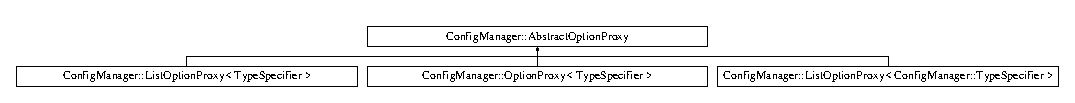
\includegraphics[height=0.933333cm]{class_config_manager_1_1_abstract_option_proxy}
\end{center}
\end{figure}
\subsection*{Public Member Functions}
\begin{DoxyCompactItemize}
\item 
const std\+::string \& \hyperlink{class_config_manager_1_1_abstract_option_proxy_a0229c3458ea6c098f27e6b98d4313840}{Get\+Name} ()
\item 
const std\+::string \& \hyperlink{class_config_manager_1_1_abstract_option_proxy_ab72b714dd0e136a5816336147a59b480}{Get\+Section\+Name} ()
\end{DoxyCompactItemize}
\subsection*{Protected Member Functions}
\begin{DoxyCompactItemize}
\item 
\hyperlink{class_config_manager_1_1_abstract_option_proxy_a892c7a737516fc69c7fd01440bfb2fa7}{Abstract\+Option\+Proxy} ()
\item 
{\bfseries Abstract\+Option\+Proxy} (\hyperlink{class_config_manager_1_1_option_node}{Option\+Node} \&option\+\_\+node)\hypertarget{class_config_manager_1_1_abstract_option_proxy_af60007dcca013f8619f9500b0a8316bf}{}\label{class_config_manager_1_1_abstract_option_proxy_af60007dcca013f8619f9500b0a8316bf}

\item 
\hyperlink{class_config_manager_1_1_abstract_option_proxy_a127ae61038607c8f850a09a2c1bffefe}{Abstract\+Option\+Proxy} (const \hyperlink{class_config_manager_1_1_abstract_option_proxy}{Abstract\+Option\+Proxy} \&other)=delete
\item 
\hyperlink{class_config_manager_1_1_abstract_option_proxy}{Abstract\+Option\+Proxy} \& \hyperlink{class_config_manager_1_1_abstract_option_proxy_aa2cddf7cb3fb32941808f45e53fa1d3b}{operator=} (const \hyperlink{class_config_manager_1_1_abstract_option_proxy}{Abstract\+Option\+Proxy} \&other)=delete
\item 
\hyperlink{class_config_manager_1_1_abstract_option_proxy_a43a75c9c184c9f5c986801a7e81ccc9d}{Abstract\+Option\+Proxy} (\hyperlink{class_config_manager_1_1_abstract_option_proxy}{Abstract\+Option\+Proxy} \&\&other)
\item 
\hyperlink{class_config_manager_1_1_abstract_option_proxy}{Abstract\+Option\+Proxy} \& \hyperlink{class_config_manager_1_1_abstract_option_proxy_a1b5c9f82b9fbe625006862253b5686e4}{operator=} (\hyperlink{class_config_manager_1_1_abstract_option_proxy}{Abstract\+Option\+Proxy} \&\&other)
\item 
\hyperlink{class_config_manager_1_1_abstract_option_proxy_ac82c93ad6f86967d8d5d82b7f3a84f44}{$\sim$\+Abstract\+Option\+Proxy} ()
\item 
virtual void \hyperlink{class_config_manager_1_1_abstract_option_proxy_aceb7b5e86f60c3dbd5b0622a230da1b3}{Regenerate\+Value\+Data} ()=0
\item 
virtual void \hyperlink{class_config_manager_1_1_abstract_option_proxy_aeac427f8ddac8a9c17822022a3b1aaf1}{Process\+Value\+Data} (const std\+::string \&data)=0
\item 
void \hyperlink{class_config_manager_1_1_abstract_option_proxy_ade2601420120e89e6c84df157ed7d011}{Assign\+Value\+Data} (const std\+::string \&data)
\end{DoxyCompactItemize}
\subsection*{Friends}
\begin{DoxyCompactItemize}
\item 
class {\bfseries Section}\hypertarget{class_config_manager_1_1_abstract_option_proxy_a0bd6fc422149e1c8416770631b28d40c}{}\label{class_config_manager_1_1_abstract_option_proxy_a0bd6fc422149e1c8416770631b28d40c}

\item 
class {\bfseries Option\+Node}\hypertarget{class_config_manager_1_1_abstract_option_proxy_a4a7f225bb7604703c1fb0023c85c7f28}{}\label{class_config_manager_1_1_abstract_option_proxy_a4a7f225bb7604703c1fb0023c85c7f28}

\end{DoxyCompactItemize}


\subsection{Detailed Description}
Spolecny predek trid \hyperlink{class_config_manager_1_1_option_proxy}{Option\+Proxy} a \hyperlink{class_config_manager_1_1_list_option_proxy}{List\+Option\+Proxy}. Virtualni trida. Zastresuje spolecne chovani trid \hyperlink{class_config_manager_1_1_option_proxy}{Option\+Proxy} a \hyperlink{class_config_manager_1_1_list_option_proxy}{List\+Option\+Proxy}. Specialni konstruktory zajistuji pouze \char`\"{}non-\/copyable\char`\"{} chovani. 

Definition at line 17 of file option.\+h.



\subsection{Constructor \& Destructor Documentation}
\index{Config\+Manager\+::\+Abstract\+Option\+Proxy@{Config\+Manager\+::\+Abstract\+Option\+Proxy}!Abstract\+Option\+Proxy@{Abstract\+Option\+Proxy}}
\index{Abstract\+Option\+Proxy@{Abstract\+Option\+Proxy}!Config\+Manager\+::\+Abstract\+Option\+Proxy@{Config\+Manager\+::\+Abstract\+Option\+Proxy}}
\subsubsection[{\texorpdfstring{Abstract\+Option\+Proxy()}{AbstractOptionProxy()}}]{\setlength{\rightskip}{0pt plus 5cm}Config\+Manager\+::\+Abstract\+Option\+Proxy\+::\+Abstract\+Option\+Proxy (
\begin{DoxyParamCaption}
{}
\end{DoxyParamCaption}
)\hspace{0.3cm}{\ttfamily [protected]}}\hypertarget{class_config_manager_1_1_abstract_option_proxy_a892c7a737516fc69c7fd01440bfb2fa7}{}\label{class_config_manager_1_1_abstract_option_proxy_a892c7a737516fc69c7fd01440bfb2fa7}
Zakladn� konstruktor. 

Definition at line 8 of file option.\+cpp.

\index{Config\+Manager\+::\+Abstract\+Option\+Proxy@{Config\+Manager\+::\+Abstract\+Option\+Proxy}!Abstract\+Option\+Proxy@{Abstract\+Option\+Proxy}}
\index{Abstract\+Option\+Proxy@{Abstract\+Option\+Proxy}!Config\+Manager\+::\+Abstract\+Option\+Proxy@{Config\+Manager\+::\+Abstract\+Option\+Proxy}}
\subsubsection[{\texorpdfstring{Abstract\+Option\+Proxy(const Abstract\+Option\+Proxy \&other)=delete}{AbstractOptionProxy(const AbstractOptionProxy &other)=delete}}]{\setlength{\rightskip}{0pt plus 5cm}Config\+Manager\+::\+Abstract\+Option\+Proxy\+::\+Abstract\+Option\+Proxy (
\begin{DoxyParamCaption}
\item[{const {\bf Abstract\+Option\+Proxy} \&}]{other}
\end{DoxyParamCaption}
)\hspace{0.3cm}{\ttfamily [protected]}, {\ttfamily [delete]}}\hypertarget{class_config_manager_1_1_abstract_option_proxy_a127ae61038607c8f850a09a2c1bffefe}{}\label{class_config_manager_1_1_abstract_option_proxy_a127ae61038607c8f850a09a2c1bffefe}
Neni povoleno kopirovani instanci teto tridy. \index{Config\+Manager\+::\+Abstract\+Option\+Proxy@{Config\+Manager\+::\+Abstract\+Option\+Proxy}!Abstract\+Option\+Proxy@{Abstract\+Option\+Proxy}}
\index{Abstract\+Option\+Proxy@{Abstract\+Option\+Proxy}!Config\+Manager\+::\+Abstract\+Option\+Proxy@{Config\+Manager\+::\+Abstract\+Option\+Proxy}}
\subsubsection[{\texorpdfstring{Abstract\+Option\+Proxy(\+Abstract\+Option\+Proxy \&\&other)}{AbstractOptionProxy(AbstractOptionProxy &&other)}}]{\setlength{\rightskip}{0pt plus 5cm}Config\+Manager\+::\+Abstract\+Option\+Proxy\+::\+Abstract\+Option\+Proxy (
\begin{DoxyParamCaption}
\item[{{\bf Abstract\+Option\+Proxy} \&\&}]{other}
\end{DoxyParamCaption}
)\hspace{0.3cm}{\ttfamily [protected]}}\hypertarget{class_config_manager_1_1_abstract_option_proxy_a43a75c9c184c9f5c986801a7e81ccc9d}{}\label{class_config_manager_1_1_abstract_option_proxy_a43a75c9c184c9f5c986801a7e81ccc9d}
Je povoleno pouze \char`\"{}movable\char`\"{} chovani. 

Definition at line 27 of file option.\+cpp.

\index{Config\+Manager\+::\+Abstract\+Option\+Proxy@{Config\+Manager\+::\+Abstract\+Option\+Proxy}!````~Abstract\+Option\+Proxy@{$\sim$\+Abstract\+Option\+Proxy}}
\index{````~Abstract\+Option\+Proxy@{$\sim$\+Abstract\+Option\+Proxy}!Config\+Manager\+::\+Abstract\+Option\+Proxy@{Config\+Manager\+::\+Abstract\+Option\+Proxy}}
\subsubsection[{\texorpdfstring{$\sim$\+Abstract\+Option\+Proxy()}{~AbstractOptionProxy()}}]{\setlength{\rightskip}{0pt plus 5cm}Config\+Manager\+::\+Abstract\+Option\+Proxy\+::$\sim$\+Abstract\+Option\+Proxy (
\begin{DoxyParamCaption}
{}
\end{DoxyParamCaption}
)\hspace{0.3cm}{\ttfamily [protected]}}\hypertarget{class_config_manager_1_1_abstract_option_proxy_ac82c93ad6f86967d8d5d82b7f3a84f44}{}\label{class_config_manager_1_1_abstract_option_proxy_ac82c93ad6f86967d8d5d82b7f3a84f44}
Zakladni destruktor. 

Definition at line 51 of file option.\+cpp.



\subsection{Member Function Documentation}
\index{Config\+Manager\+::\+Abstract\+Option\+Proxy@{Config\+Manager\+::\+Abstract\+Option\+Proxy}!Assign\+Value\+Data@{Assign\+Value\+Data}}
\index{Assign\+Value\+Data@{Assign\+Value\+Data}!Config\+Manager\+::\+Abstract\+Option\+Proxy@{Config\+Manager\+::\+Abstract\+Option\+Proxy}}
\subsubsection[{\texorpdfstring{Assign\+Value\+Data(const std\+::string \&data)}{AssignValueData(const std::string &data)}}]{\setlength{\rightskip}{0pt plus 5cm}void Config\+Manager\+::\+Abstract\+Option\+Proxy\+::\+Assign\+Value\+Data (
\begin{DoxyParamCaption}
\item[{const std\+::string \&}]{data}
\end{DoxyParamCaption}
)\hspace{0.3cm}{\ttfamily [protected]}}\hypertarget{class_config_manager_1_1_abstract_option_proxy_ade2601420120e89e6c84df157ed7d011}{}\label{class_config_manager_1_1_abstract_option_proxy_ade2601420120e89e6c84df157ed7d011}
Metoda pro komunikaci s \hyperlink{class_config_manager_1_1_configuration}{Configuration} slouzici k nastaveni hodnoty z Option\+Proxyu do retezcove hodnoty v \hyperlink{class_config_manager_1_1_configuration}{Configuration}, iniciovane v potomcich Option\+Proxyu. 
\begin{DoxyParams}{Parameters}
{\em Textova} & data ktera maji prepsat retezcove hodnoty v \hyperlink{class_config_manager_1_1_configuration}{Configuration}. \\
\hline
\end{DoxyParams}


Definition at line 59 of file option.\+cpp.

\index{Config\+Manager\+::\+Abstract\+Option\+Proxy@{Config\+Manager\+::\+Abstract\+Option\+Proxy}!Get\+Name@{Get\+Name}}
\index{Get\+Name@{Get\+Name}!Config\+Manager\+::\+Abstract\+Option\+Proxy@{Config\+Manager\+::\+Abstract\+Option\+Proxy}}
\subsubsection[{\texorpdfstring{Get\+Name()}{GetName()}}]{\setlength{\rightskip}{0pt plus 5cm}const std\+::string \& Config\+Manager\+::\+Abstract\+Option\+Proxy\+::\+Get\+Name (
\begin{DoxyParamCaption}
{}
\end{DoxyParamCaption}
)}\hypertarget{class_config_manager_1_1_abstract_option_proxy_a0229c3458ea6c098f27e6b98d4313840}{}\label{class_config_manager_1_1_abstract_option_proxy_a0229c3458ea6c098f27e6b98d4313840}
Tato metoda vraci nazev optionu. 

Definition at line 80 of file option.\+cpp.

\index{Config\+Manager\+::\+Abstract\+Option\+Proxy@{Config\+Manager\+::\+Abstract\+Option\+Proxy}!Get\+Section\+Name@{Get\+Section\+Name}}
\index{Get\+Section\+Name@{Get\+Section\+Name}!Config\+Manager\+::\+Abstract\+Option\+Proxy@{Config\+Manager\+::\+Abstract\+Option\+Proxy}}
\subsubsection[{\texorpdfstring{Get\+Section\+Name()}{GetSectionName()}}]{\setlength{\rightskip}{0pt plus 5cm}const std\+::string \& Config\+Manager\+::\+Abstract\+Option\+Proxy\+::\+Get\+Section\+Name (
\begin{DoxyParamCaption}
{}
\end{DoxyParamCaption}
)}\hypertarget{class_config_manager_1_1_abstract_option_proxy_ab72b714dd0e136a5816336147a59b480}{}\label{class_config_manager_1_1_abstract_option_proxy_ab72b714dd0e136a5816336147a59b480}
Metoda zpristupnujici jmeno sekce do ktere tento option prislusi. 

Definition at line 92 of file option.\+cpp.

\index{Config\+Manager\+::\+Abstract\+Option\+Proxy@{Config\+Manager\+::\+Abstract\+Option\+Proxy}!operator=@{operator=}}
\index{operator=@{operator=}!Config\+Manager\+::\+Abstract\+Option\+Proxy@{Config\+Manager\+::\+Abstract\+Option\+Proxy}}
\subsubsection[{\texorpdfstring{operator=(const Abstract\+Option\+Proxy \&other)=delete}{operator=(const AbstractOptionProxy &other)=delete}}]{\setlength{\rightskip}{0pt plus 5cm}{\bf Abstract\+Option\+Proxy}\& Config\+Manager\+::\+Abstract\+Option\+Proxy\+::operator= (
\begin{DoxyParamCaption}
\item[{const {\bf Abstract\+Option\+Proxy} \&}]{other}
\end{DoxyParamCaption}
)\hspace{0.3cm}{\ttfamily [protected]}, {\ttfamily [delete]}}\hypertarget{class_config_manager_1_1_abstract_option_proxy_aa2cddf7cb3fb32941808f45e53fa1d3b}{}\label{class_config_manager_1_1_abstract_option_proxy_aa2cddf7cb3fb32941808f45e53fa1d3b}
Neni povoleno kopirovani instanci teto tridy. \index{Config\+Manager\+::\+Abstract\+Option\+Proxy@{Config\+Manager\+::\+Abstract\+Option\+Proxy}!operator=@{operator=}}
\index{operator=@{operator=}!Config\+Manager\+::\+Abstract\+Option\+Proxy@{Config\+Manager\+::\+Abstract\+Option\+Proxy}}
\subsubsection[{\texorpdfstring{operator=(\+Abstract\+Option\+Proxy \&\&other)}{operator=(AbstractOptionProxy &&other)}}]{\setlength{\rightskip}{0pt plus 5cm}{\bf Abstract\+Option\+Proxy} \& Config\+Manager\+::\+Abstract\+Option\+Proxy\+::operator= (
\begin{DoxyParamCaption}
\item[{{\bf Abstract\+Option\+Proxy} \&\&}]{other}
\end{DoxyParamCaption}
)\hspace{0.3cm}{\ttfamily [protected]}}\hypertarget{class_config_manager_1_1_abstract_option_proxy_a1b5c9f82b9fbe625006862253b5686e4}{}\label{class_config_manager_1_1_abstract_option_proxy_a1b5c9f82b9fbe625006862253b5686e4}




Je povoleno pouze \char`\"{}movable\char`\"{} chovani. 

Definition at line 36 of file option.\+cpp.

\index{Config\+Manager\+::\+Abstract\+Option\+Proxy@{Config\+Manager\+::\+Abstract\+Option\+Proxy}!Process\+Value\+Data@{Process\+Value\+Data}}
\index{Process\+Value\+Data@{Process\+Value\+Data}!Config\+Manager\+::\+Abstract\+Option\+Proxy@{Config\+Manager\+::\+Abstract\+Option\+Proxy}}
\subsubsection[{\texorpdfstring{Process\+Value\+Data(const std\+::string \&data)=0}{ProcessValueData(const std::string &data)=0}}]{\setlength{\rightskip}{0pt plus 5cm}virtual void Config\+Manager\+::\+Abstract\+Option\+Proxy\+::\+Process\+Value\+Data (
\begin{DoxyParamCaption}
\item[{const std\+::string \&}]{data}
\end{DoxyParamCaption}
)\hspace{0.3cm}{\ttfamily [protected]}, {\ttfamily [pure virtual]}}\hypertarget{class_config_manager_1_1_abstract_option_proxy_aeac427f8ddac8a9c17822022a3b1aaf1}{}\label{class_config_manager_1_1_abstract_option_proxy_aeac427f8ddac8a9c17822022a3b1aaf1}
Metoda pro komunikaci s \hyperlink{class_config_manager_1_1_configuration}{Configuration} slouzici k aktualizaci hodnoty v Option\+Proxyu dle retezcove hodnoty v \hyperlink{class_config_manager_1_1_configuration}{Configuration}, iniciovane v \hyperlink{class_config_manager_1_1_configuration}{Configuration} (pripadne \hyperlink{class_config_manager_1_1_section}{Section}). 
\begin{DoxyParams}{Parameters}
{\em data} & Text ze ktereho ma byt hodnota prectena. \\
\hline
\end{DoxyParams}


Implemented in \hyperlink{class_config_manager_1_1_list_option_proxy_ade1da6bf53c9bef0806755e4f805284e}{Config\+Manager\+::\+List\+Option\+Proxy$<$ Type\+Specifier $>$}, \hyperlink{class_config_manager_1_1_list_option_proxy_ade1da6bf53c9bef0806755e4f805284e}{Config\+Manager\+::\+List\+Option\+Proxy$<$ Config\+Manager\+::\+Type\+Specifier $>$}, and \hyperlink{class_config_manager_1_1_option_proxy_a41e884af79ba112250af76538cc38dc1}{Config\+Manager\+::\+Option\+Proxy$<$ Type\+Specifier $>$}.

\index{Config\+Manager\+::\+Abstract\+Option\+Proxy@{Config\+Manager\+::\+Abstract\+Option\+Proxy}!Regenerate\+Value\+Data@{Regenerate\+Value\+Data}}
\index{Regenerate\+Value\+Data@{Regenerate\+Value\+Data}!Config\+Manager\+::\+Abstract\+Option\+Proxy@{Config\+Manager\+::\+Abstract\+Option\+Proxy}}
\subsubsection[{\texorpdfstring{Regenerate\+Value\+Data()=0}{RegenerateValueData()=0}}]{\setlength{\rightskip}{0pt plus 5cm}virtual void Config\+Manager\+::\+Abstract\+Option\+Proxy\+::\+Regenerate\+Value\+Data (
\begin{DoxyParamCaption}
{}
\end{DoxyParamCaption}
)\hspace{0.3cm}{\ttfamily [protected]}, {\ttfamily [pure virtual]}}\hypertarget{class_config_manager_1_1_abstract_option_proxy_aceb7b5e86f60c3dbd5b0622a230da1b3}{}\label{class_config_manager_1_1_abstract_option_proxy_aceb7b5e86f60c3dbd5b0622a230da1b3}
Metoda pro komunikaci s \hyperlink{class_config_manager_1_1_configuration}{Configuration} slouzici pro vyvolani prepsani aktualni hodnoty v \hyperlink{class_config_manager_1_1_configuration}{Configuration} retezcovou reprezentaci hodnoty v Option\+Proxyu (lze tim zapsat default), iniciovane v \hyperlink{class_config_manager_1_1_configuration}{Configuration}. 

Implemented in \hyperlink{class_config_manager_1_1_list_option_proxy_ab7d04f2f12da920861c6cef6d8dca501}{Config\+Manager\+::\+List\+Option\+Proxy$<$ Type\+Specifier $>$}, \hyperlink{class_config_manager_1_1_list_option_proxy_ab7d04f2f12da920861c6cef6d8dca501}{Config\+Manager\+::\+List\+Option\+Proxy$<$ Config\+Manager\+::\+Type\+Specifier $>$}, and \hyperlink{class_config_manager_1_1_option_proxy_a6f0f8c517701e7f55c2572e2deae6ad9}{Config\+Manager\+::\+Option\+Proxy$<$ Type\+Specifier $>$}.



The documentation for this class was generated from the following files\+:\begin{DoxyCompactItemize}
\item 
E\+:/\+I\+N\+F\+O\+R\+M\+A\+T\+I\+K\+A/doporucene\+Postupy/uloha4/repos/src/\+Config\+Manager/option.\+h\item 
E\+:/\+I\+N\+F\+O\+R\+M\+A\+T\+I\+K\+A/doporucene\+Postupy/uloha4/repos/src/\+Config\+Manager/option.\+cpp\end{DoxyCompactItemize}

\hypertarget{class_config_manager_1_1_boolean_specifier}{}\section{Config\+Manager\+:\+:Boolean\+Specifier Class Reference}
\label{class_config_manager_1_1_boolean_specifier}\index{Config\+Manager\+::\+Boolean\+Specifier@{Config\+Manager\+::\+Boolean\+Specifier}}


{\ttfamily \#include $<$typespecifiers.\+h$>$}

\subsection*{Public Types}
\begin{DoxyCompactItemize}
\item 
typedef bool \hyperlink{class_config_manager_1_1_boolean_specifier_a765f3a2d8461a647ba1a84434665b54b}{Value\+Type}
\end{DoxyCompactItemize}
\subsection*{Public Member Functions}
\begin{DoxyCompactItemize}
\item 
\hyperlink{class_config_manager_1_1_boolean_specifier_ab8c8434a5de2cccb032cb6c7fbf3ae1c}{Boolean\+Specifier} ()
\item 
\hyperlink{class_config_manager_1_1_boolean_specifier_a765f3a2d8461a647ba1a84434665b54b}{Value\+Type} \hyperlink{class_config_manager_1_1_boolean_specifier_aa2964b687c6614053a9441b8f16eadcd}{From\+String} (const std\+::string \&data)
\item 
std\+::string \hyperlink{class_config_manager_1_1_boolean_specifier_a79947088ce64f51e90b42fc27587e503}{To\+String} (\hyperlink{class_config_manager_1_1_boolean_specifier_a765f3a2d8461a647ba1a84434665b54b}{Value\+Type} value)
\end{DoxyCompactItemize}


\subsection{Detailed Description}
Trida realizujici prevod z textu do typu boolean a zpet. 

Definition at line 65 of file typespecifiers.\+h.



\subsection{Member Typedef Documentation}
\index{Config\+Manager\+::\+Boolean\+Specifier@{Config\+Manager\+::\+Boolean\+Specifier}!Value\+Type@{Value\+Type}}
\index{Value\+Type@{Value\+Type}!Config\+Manager\+::\+Boolean\+Specifier@{Config\+Manager\+::\+Boolean\+Specifier}}
\subsubsection[{\texorpdfstring{Value\+Type}{ValueType}}]{\setlength{\rightskip}{0pt plus 5cm}typedef bool {\bf Config\+Manager\+::\+Boolean\+Specifier\+::\+Value\+Type}}\hypertarget{class_config_manager_1_1_boolean_specifier_a765f3a2d8461a647ba1a84434665b54b}{}\label{class_config_manager_1_1_boolean_specifier_a765f3a2d8461a647ba1a84434665b54b}




Tato definice typu urcuje navratovy typ. 

Definition at line 71 of file typespecifiers.\+h.



\subsection{Constructor \& Destructor Documentation}
\index{Config\+Manager\+::\+Boolean\+Specifier@{Config\+Manager\+::\+Boolean\+Specifier}!Boolean\+Specifier@{Boolean\+Specifier}}
\index{Boolean\+Specifier@{Boolean\+Specifier}!Config\+Manager\+::\+Boolean\+Specifier@{Config\+Manager\+::\+Boolean\+Specifier}}
\subsubsection[{\texorpdfstring{Boolean\+Specifier()}{BooleanSpecifier()}}]{\setlength{\rightskip}{0pt plus 5cm}Config\+Manager\+::\+Boolean\+Specifier\+::\+Boolean\+Specifier (
\begin{DoxyParamCaption}
{}
\end{DoxyParamCaption}
)}\hypertarget{class_config_manager_1_1_boolean_specifier_ab8c8434a5de2cccb032cb6c7fbf3ae1c}{}\label{class_config_manager_1_1_boolean_specifier_ab8c8434a5de2cccb032cb6c7fbf3ae1c}
Zakladni konstruktor. 

Definition at line 42 of file typespecifiers.\+cpp.



\subsection{Member Function Documentation}
\index{Config\+Manager\+::\+Boolean\+Specifier@{Config\+Manager\+::\+Boolean\+Specifier}!From\+String@{From\+String}}
\index{From\+String@{From\+String}!Config\+Manager\+::\+Boolean\+Specifier@{Config\+Manager\+::\+Boolean\+Specifier}}
\subsubsection[{\texorpdfstring{From\+String(const std\+::string \&data)}{FromString(const std::string &data)}}]{\setlength{\rightskip}{0pt plus 5cm}{\bf Boolean\+Specifier\+::\+Value\+Type} Config\+Manager\+::\+Boolean\+Specifier\+::\+From\+String (
\begin{DoxyParamCaption}
\item[{const std\+::string \&}]{data}
\end{DoxyParamCaption}
)}\hypertarget{class_config_manager_1_1_boolean_specifier_aa2964b687c6614053a9441b8f16eadcd}{}\label{class_config_manager_1_1_boolean_specifier_aa2964b687c6614053a9441b8f16eadcd}




Metoda prevadejici text na vyslednou hodnotu. Muze vyhodit \hyperlink{class_config_manager_1_1_wrong_format_exception}{Wrong\+Format\+Exception} vyjimku. 
\begin{DoxyParams}{Parameters}
{\em data} & Vstupni data. \\
\hline
\end{DoxyParams}


Definition at line 46 of file typespecifiers.\+cpp.

\index{Config\+Manager\+::\+Boolean\+Specifier@{Config\+Manager\+::\+Boolean\+Specifier}!To\+String@{To\+String}}
\index{To\+String@{To\+String}!Config\+Manager\+::\+Boolean\+Specifier@{Config\+Manager\+::\+Boolean\+Specifier}}
\subsubsection[{\texorpdfstring{To\+String(\+Value\+Type value)}{ToString(ValueType value)}}]{\setlength{\rightskip}{0pt plus 5cm}std\+::string Config\+Manager\+::\+Boolean\+Specifier\+::\+To\+String (
\begin{DoxyParamCaption}
\item[{{\bf Boolean\+Specifier\+::\+Value\+Type}}]{value}
\end{DoxyParamCaption}
)}\hypertarget{class_config_manager_1_1_boolean_specifier_a79947088ce64f51e90b42fc27587e503}{}\label{class_config_manager_1_1_boolean_specifier_a79947088ce64f51e90b42fc27587e503}




Metoda prevadejici nastavenou/zmenenou hodnotu zpet do textoveho formatu. Muze vyhodit \hyperlink{class_config_manager_1_1_wrong_format_exception}{Wrong\+Format\+Exception} vyjimku. 
\begin{DoxyParams}{Parameters}
{\em Hodnota} & preveditelna na string. \\
\hline
\end{DoxyParams}


Definition at line 76 of file typespecifiers.\+cpp.



The documentation for this class was generated from the following files\+:\begin{DoxyCompactItemize}
\item 
src/\+Config\+Manager/typespecifiers.\+h\item 
src/\+Config\+Manager/typespecifiers.\+cpp\end{DoxyCompactItemize}

\hypertarget{class_test_1_1_collector_output}{}\section{Test\+:\+:Collector\+Output Class Reference}
\label{class_test_1_1_collector_output}\index{Test\+::\+Collector\+Output@{Test\+::\+Collector\+Output}}


Collector output.  




{\ttfamily \#include $<$cpptest-\/collectoroutput.\+h$>$}

Inheritance diagram for Test\+:\+:Collector\+Output\+:\begin{figure}[H]
\begin{center}
\leavevmode
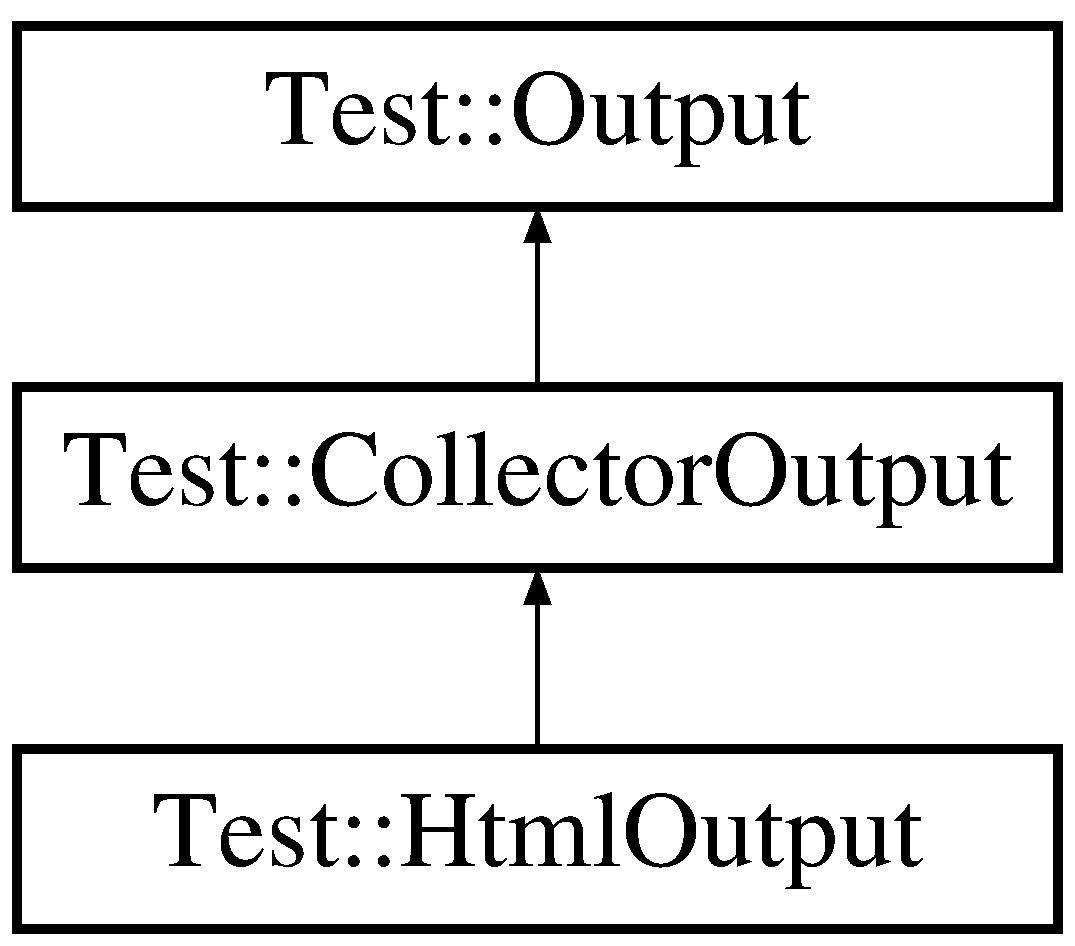
\includegraphics[height=3.000000cm]{class_test_1_1_collector_output}
\end{center}
\end{figure}
\subsection*{Classes}
\begin{DoxyCompactItemize}
\item 
struct \hyperlink{struct_test_1_1_collector_output_1_1_suite_info}{Suite\+Info}
\item 
struct \hyperlink{struct_test_1_1_collector_output_1_1_test_info}{Test\+Info}
\end{DoxyCompactItemize}
\subsection*{Public Member Functions}
\begin{DoxyCompactItemize}
\item 
virtual void \hyperlink{class_test_1_1_collector_output_a758efaaf1e348636cb3877c622d2b5d0}{finished} (int tests, const \hyperlink{class_test_1_1_time}{Time} \&time)
\item 
virtual void \hyperlink{class_test_1_1_collector_output_ab4ea305009efd9e56c0549a04c9d55e6}{suite\+\_\+start} (int tests, const std\+::string \&name)
\item 
virtual void \hyperlink{class_test_1_1_collector_output_a25d129d55214c92189265a7bccd5b2cd}{suite\+\_\+end} (int tests, const std\+::string \&name, const \hyperlink{class_test_1_1_time}{Time} \&time)
\item 
virtual void \hyperlink{class_test_1_1_collector_output_a512aa60f06439a22c41dc5c3bfca15ff}{test\+\_\+start} (const std\+::string \&name)
\item 
virtual void \hyperlink{class_test_1_1_collector_output_aa6f64879932cde17fc0098b8fc197c62}{test\+\_\+end} (const std\+::string \&name, bool ok, const \hyperlink{class_test_1_1_time}{Time} \&time)
\item 
virtual void \hyperlink{class_test_1_1_collector_output_a201ecd71ad6e443b0be2e987d2dc3b39}{assertment} (const \hyperlink{class_test_1_1_source}{Source} \&s)
\end{DoxyCompactItemize}
\subsection*{Protected Types}
\begin{DoxyCompactItemize}
\item 
typedef std\+::list$<$ \hyperlink{class_test_1_1_source}{Source} $>$ {\bfseries Sources}\hypertarget{class_test_1_1_collector_output_a1921f35e0da596bd75da5824afe872c9}{}\label{class_test_1_1_collector_output_a1921f35e0da596bd75da5824afe872c9}

\item 
typedef std\+::vector$<$ \hyperlink{struct_test_1_1_collector_output_1_1_test_info}{Test\+Info} $>$ {\bfseries Tests}\hypertarget{class_test_1_1_collector_output_a54a7b7c9b6d181102bc8934190b06e86}{}\label{class_test_1_1_collector_output_a54a7b7c9b6d181102bc8934190b06e86}

\item 
typedef std\+::list$<$ \hyperlink{struct_test_1_1_collector_output_1_1_suite_info}{Suite\+Info} $>$ {\bfseries Suites}\hypertarget{class_test_1_1_collector_output_a0879ce3b51f1e3b3fe14aa5665dccd30}{}\label{class_test_1_1_collector_output_a0879ce3b51f1e3b3fe14aa5665dccd30}

\end{DoxyCompactItemize}
\subsection*{Protected Member Functions}
\begin{DoxyCompactItemize}
\item 
\hyperlink{class_test_1_1_collector_output_a852bde8f194b4f81ca36f222257adc53}{Collector\+Output} ()
\end{DoxyCompactItemize}
\subsection*{Protected Attributes}
\begin{DoxyCompactItemize}
\item 
Suites {\bfseries \+\_\+suites}\hypertarget{class_test_1_1_collector_output_a9f79c0fa5abf1d6248a85e7ae4701c5f}{}\label{class_test_1_1_collector_output_a9f79c0fa5abf1d6248a85e7ae4701c5f}

\item 
int {\bfseries \+\_\+total\+\_\+errors}\hypertarget{class_test_1_1_collector_output_a7d8ec4ad0316b57aa96ae50a548c94d2}{}\label{class_test_1_1_collector_output_a7d8ec4ad0316b57aa96ae50a548c94d2}

\item 
int {\bfseries \+\_\+total\+\_\+tests}\hypertarget{class_test_1_1_collector_output_ace6c1fc02a6ac7a6c15b982b96f5f68f}{}\label{class_test_1_1_collector_output_ace6c1fc02a6ac7a6c15b982b96f5f68f}

\item 
\hyperlink{class_test_1_1_time}{Time} {\bfseries \+\_\+total\+\_\+time}\hypertarget{class_test_1_1_collector_output_af1e014fde4bf5b4e6c89de748630aa79}{}\label{class_test_1_1_collector_output_af1e014fde4bf5b4e6c89de748630aa79}

\end{DoxyCompactItemize}


\subsection{Detailed Description}
Collector output. 

Base class for output handlers that need to report status when all tests have executed. 

Definition at line 47 of file cpptest-\/collectoroutput.\+h.



\subsection{Constructor \& Destructor Documentation}
\index{Test\+::\+Collector\+Output@{Test\+::\+Collector\+Output}!Collector\+Output@{Collector\+Output}}
\index{Collector\+Output@{Collector\+Output}!Test\+::\+Collector\+Output@{Test\+::\+Collector\+Output}}
\subsubsection[{\texorpdfstring{Collector\+Output()}{CollectorOutput()}}]{\setlength{\rightskip}{0pt plus 5cm}Test\+::\+Collector\+Output\+::\+Collector\+Output (
\begin{DoxyParamCaption}
{}
\end{DoxyParamCaption}
)\hspace{0.3cm}{\ttfamily [protected]}}\hypertarget{class_test_1_1_collector_output_a852bde8f194b4f81ca36f222257adc53}{}\label{class_test_1_1_collector_output_a852bde8f194b4f81ca36f222257adc53}
Constructs a collector object. 

Definition at line 52 of file collectoroutput.\+cpp.



\subsection{Member Function Documentation}
\index{Test\+::\+Collector\+Output@{Test\+::\+Collector\+Output}!assertment@{assertment}}
\index{assertment@{assertment}!Test\+::\+Collector\+Output@{Test\+::\+Collector\+Output}}
\subsubsection[{\texorpdfstring{assertment(const Source \&s)}{assertment(const Source &s)}}]{\setlength{\rightskip}{0pt plus 5cm}void Test\+::\+Collector\+Output\+::assertment (
\begin{DoxyParamCaption}
\item[{const {\bf Source} \&}]{s}
\end{DoxyParamCaption}
)\hspace{0.3cm}{\ttfamily [virtual]}}\hypertarget{class_test_1_1_collector_output_a201ecd71ad6e443b0be2e987d2dc3b39}{}\label{class_test_1_1_collector_output_a201ecd71ad6e443b0be2e987d2dc3b39}
Called when an assertment is issued.


\begin{DoxyParams}{Parameters}
{\em s} & Assert point information. \\
\hline
\end{DoxyParams}


Reimplemented from \hyperlink{class_test_1_1_output_a48c31f0baa7627d81939be840c9a7f65}{Test\+::\+Output}.



Definition at line 100 of file collectoroutput.\+cpp.

\index{Test\+::\+Collector\+Output@{Test\+::\+Collector\+Output}!finished@{finished}}
\index{finished@{finished}!Test\+::\+Collector\+Output@{Test\+::\+Collector\+Output}}
\subsubsection[{\texorpdfstring{finished(int tests, const Time \&time)}{finished(int tests, const Time &time)}}]{\setlength{\rightskip}{0pt plus 5cm}void Test\+::\+Collector\+Output\+::finished (
\begin{DoxyParamCaption}
\item[{int}]{tests, }
\item[{const {\bf Time} \&}]{time}
\end{DoxyParamCaption}
)\hspace{0.3cm}{\ttfamily [virtual]}}\hypertarget{class_test_1_1_collector_output_a758efaaf1e348636cb3877c622d2b5d0}{}\label{class_test_1_1_collector_output_a758efaaf1e348636cb3877c622d2b5d0}
Called when testing is finished.


\begin{DoxyParams}{Parameters}
{\em tests} & Total number of tests in all suites. \\
\hline
{\em time} & Total elapsed time for all tests. \\
\hline
\end{DoxyParams}


Reimplemented from \hyperlink{class_test_1_1_output_aeff8af8326a8c54a38199f76837f860a}{Test\+::\+Output}.



Definition at line 58 of file collectoroutput.\+cpp.

\index{Test\+::\+Collector\+Output@{Test\+::\+Collector\+Output}!suite\+\_\+end@{suite\+\_\+end}}
\index{suite\+\_\+end@{suite\+\_\+end}!Test\+::\+Collector\+Output@{Test\+::\+Collector\+Output}}
\subsubsection[{\texorpdfstring{suite\+\_\+end(int tests, const std\+::string \&name, const Time \&time)}{suite_end(int tests, const std::string &name, const Time &time)}}]{\setlength{\rightskip}{0pt plus 5cm}void Test\+::\+Collector\+Output\+::suite\+\_\+end (
\begin{DoxyParamCaption}
\item[{int}]{tests, }
\item[{const std\+::string \&}]{name, }
\item[{const {\bf Time} \&}]{time}
\end{DoxyParamCaption}
)\hspace{0.3cm}{\ttfamily [virtual]}}\hypertarget{class_test_1_1_collector_output_a25d129d55214c92189265a7bccd5b2cd}{}\label{class_test_1_1_collector_output_a25d129d55214c92189265a7bccd5b2cd}
Called when a suite is finished.


\begin{DoxyParams}{Parameters}
{\em tests} & Number of tests in this suite. \\
\hline
{\em name} & Name of the suite. \\
\hline
{\em time} & Total elapsed time for all tests in this suite. \\
\hline
\end{DoxyParams}


Reimplemented from \hyperlink{class_test_1_1_output_a6dbf4c0adb2bd4a7364c629179f788a6}{Test\+::\+Output}.



Definition at line 75 of file collectoroutput.\+cpp.

\index{Test\+::\+Collector\+Output@{Test\+::\+Collector\+Output}!suite\+\_\+start@{suite\+\_\+start}}
\index{suite\+\_\+start@{suite\+\_\+start}!Test\+::\+Collector\+Output@{Test\+::\+Collector\+Output}}
\subsubsection[{\texorpdfstring{suite\+\_\+start(int tests, const std\+::string \&name)}{suite_start(int tests, const std::string &name)}}]{\setlength{\rightskip}{0pt plus 5cm}void Test\+::\+Collector\+Output\+::suite\+\_\+start (
\begin{DoxyParamCaption}
\item[{int}]{tests, }
\item[{const std\+::string \&}]{name}
\end{DoxyParamCaption}
)\hspace{0.3cm}{\ttfamily [virtual]}}\hypertarget{class_test_1_1_collector_output_ab4ea305009efd9e56c0549a04c9d55e6}{}\label{class_test_1_1_collector_output_ab4ea305009efd9e56c0549a04c9d55e6}
Called when a suite is entered.


\begin{DoxyParams}{Parameters}
{\em tests} & Number of tests in this suite. \\
\hline
{\em name} & Name of the suite. \\
\hline
\end{DoxyParams}


Reimplemented from \hyperlink{class_test_1_1_output_a7022c32c5a1577b10b93d3942746f17d}{Test\+::\+Output}.



Definition at line 65 of file collectoroutput.\+cpp.

\index{Test\+::\+Collector\+Output@{Test\+::\+Collector\+Output}!test\+\_\+end@{test\+\_\+end}}
\index{test\+\_\+end@{test\+\_\+end}!Test\+::\+Collector\+Output@{Test\+::\+Collector\+Output}}
\subsubsection[{\texorpdfstring{test\+\_\+end(const std\+::string \&name, bool ok, const Time \&time)}{test_end(const std::string &name, bool ok, const Time &time)}}]{\setlength{\rightskip}{0pt plus 5cm}void Test\+::\+Collector\+Output\+::test\+\_\+end (
\begin{DoxyParamCaption}
\item[{const std\+::string \&}]{name, }
\item[{bool}]{ok, }
\item[{const {\bf Time} \&}]{time}
\end{DoxyParamCaption}
)\hspace{0.3cm}{\ttfamily [virtual]}}\hypertarget{class_test_1_1_collector_output_aa6f64879932cde17fc0098b8fc197c62}{}\label{class_test_1_1_collector_output_aa6f64879932cde17fc0098b8fc197c62}
Called when a test if finished, regardless if an assertment was issued.


\begin{DoxyParams}{Parameters}
{\em name} & Name of the test function. \\
\hline
{\em ok} & True if the test was successful; false otherwise. \\
\hline
{\em time} & Execution time. \\
\hline
\end{DoxyParams}


Reimplemented from \hyperlink{class_test_1_1_output_a3796943e3b56373492c957212a21454e}{Test\+::\+Output}.



Definition at line 92 of file collectoroutput.\+cpp.

\index{Test\+::\+Collector\+Output@{Test\+::\+Collector\+Output}!test\+\_\+start@{test\+\_\+start}}
\index{test\+\_\+start@{test\+\_\+start}!Test\+::\+Collector\+Output@{Test\+::\+Collector\+Output}}
\subsubsection[{\texorpdfstring{test\+\_\+start(const std\+::string \&name)}{test_start(const std::string &name)}}]{\setlength{\rightskip}{0pt plus 5cm}void Test\+::\+Collector\+Output\+::test\+\_\+start (
\begin{DoxyParamCaption}
\item[{const std\+::string \&}]{name}
\end{DoxyParamCaption}
)\hspace{0.3cm}{\ttfamily [virtual]}}\hypertarget{class_test_1_1_collector_output_a512aa60f06439a22c41dc5c3bfca15ff}{}\label{class_test_1_1_collector_output_a512aa60f06439a22c41dc5c3bfca15ff}
Called when a tests is executed.


\begin{DoxyParams}{Parameters}
{\em name} & Name of the test function. \\
\hline
\end{DoxyParams}


Reimplemented from \hyperlink{class_test_1_1_output_a52d43b97609febc5abbc6da9aa0abac2}{Test\+::\+Output}.



Definition at line 85 of file collectoroutput.\+cpp.



The documentation for this class was generated from the following files\+:\begin{DoxyCompactItemize}
\item 
lib/cpptest-\/1.\+1.\+2/src/\hyperlink{cpptest-collectoroutput_8h}{cpptest-\/collectoroutput.\+h}\item 
lib/cpptest-\/1.\+1.\+2/src/collectoroutput.\+cpp\end{DoxyCompactItemize}

\hypertarget{class_compare_test_suite}{}\section{Compare\+Test\+Suite Class Reference}
\label{class_compare_test_suite}\index{Compare\+Test\+Suite@{Compare\+Test\+Suite}}
Inheritance diagram for Compare\+Test\+Suite\+:\begin{figure}[H]
\begin{center}
\leavevmode
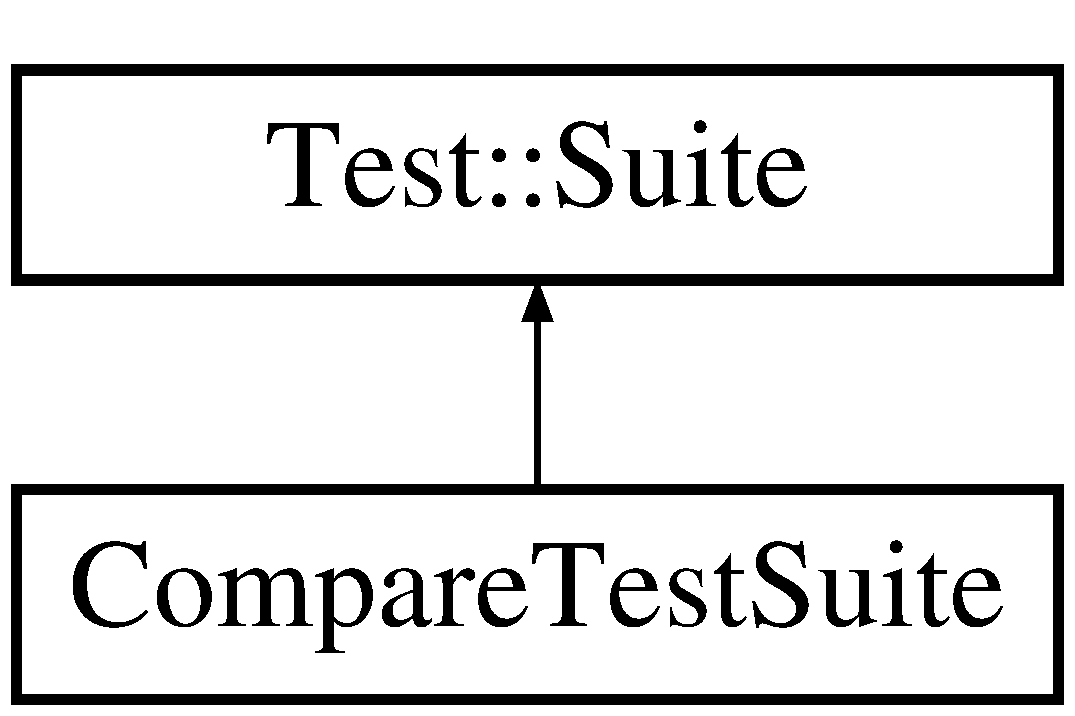
\includegraphics[height=2.000000cm]{class_compare_test_suite}
\end{center}
\end{figure}
\subsection*{Additional Inherited Members}


\subsection{Detailed Description}


Definition at line 68 of file mytest.\+cpp.



The documentation for this class was generated from the following file\+:\begin{DoxyCompactItemize}
\item 
lib/cpptest-\/1.\+1.\+2/test/mytest.\+cpp\end{DoxyCompactItemize}

\hypertarget{class_test_1_1_compiler_output}{}\section{Test\+:\+:Compiler\+Output Class Reference}
\label{class_test_1_1_compiler_output}\index{Test\+::\+Compiler\+Output@{Test\+::\+Compiler\+Output}}


Compiler-\/like output handler.  




{\ttfamily \#include $<$cpptest-\/compileroutput.\+h$>$}

Inheritance diagram for Test\+:\+:Compiler\+Output\+:\begin{figure}[H]
\begin{center}
\leavevmode
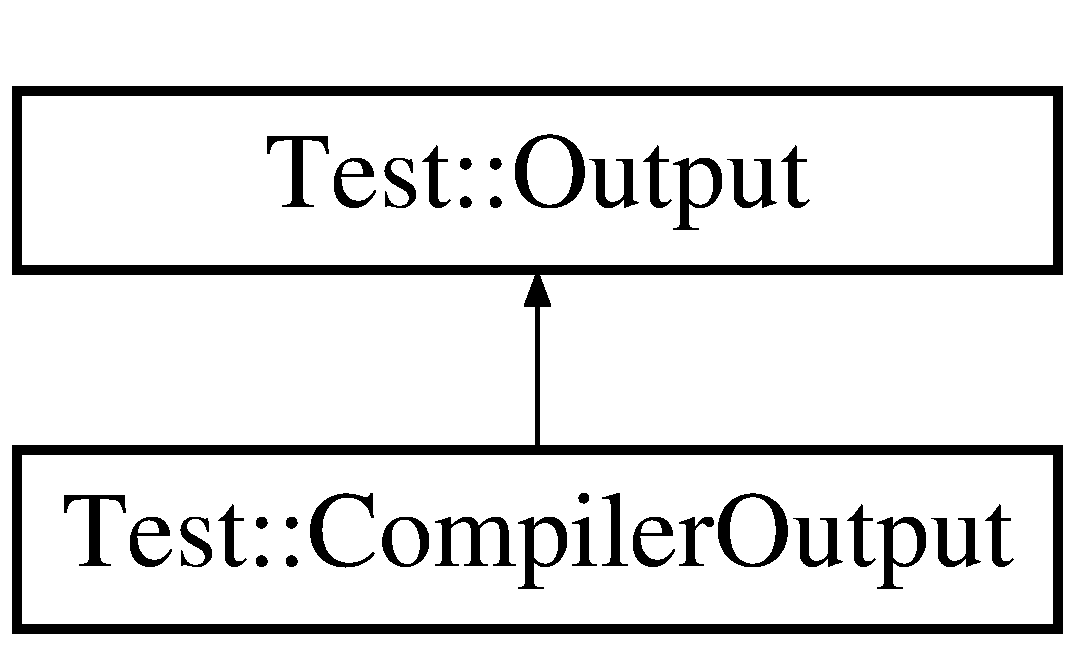
\includegraphics[height=2.000000cm]{class_test_1_1_compiler_output}
\end{center}
\end{figure}
\subsection*{Classes}
\begin{DoxyCompactItemize}
\item 
class \hyperlink{class_test_1_1_compiler_output_1_1_invalid_format}{Invalid\+Format}
\begin{DoxyCompactList}\small\item\em Compiler output exception. \end{DoxyCompactList}\end{DoxyCompactItemize}
\subsection*{Public Types}
\begin{DoxyCompactItemize}
\item 
enum \hyperlink{class_test_1_1_compiler_output_ab34cf506804cefbc67545a256af196ff}{Format} \{ \hyperlink{class_test_1_1_compiler_output_ab34cf506804cefbc67545a256af196ffa1a83926858dfb1bab06bc0a313a49dac}{Generic}, 
\hyperlink{class_test_1_1_compiler_output_ab34cf506804cefbc67545a256af196ffa9ad6dc16df2c992e8b77a3f6ee2247d8}{B\+CC}, 
\hyperlink{class_test_1_1_compiler_output_ab34cf506804cefbc67545a256af196ffa7d077829f643d60a87a022d39989dd3b}{G\+CC}, 
\hyperlink{class_test_1_1_compiler_output_ab34cf506804cefbc67545a256af196ffae4f7af0eaa05253ea35484384deeb86b}{M\+S\+VC}
 \}
\end{DoxyCompactItemize}
\subsection*{Public Member Functions}
\begin{DoxyCompactItemize}
\item 
{\bfseries Compiler\+Output} (\hyperlink{class_test_1_1_compiler_output_ab34cf506804cefbc67545a256af196ff}{Format} format=\hyperlink{class_test_1_1_compiler_output_ab34cf506804cefbc67545a256af196ffa1a83926858dfb1bab06bc0a313a49dac}{Generic}, std\+::ostream \&stream=std\+::cout)\hypertarget{class_test_1_1_compiler_output_a816ae9a0ff2fb6cbb95c7cd815a6e621}{}\label{class_test_1_1_compiler_output_a816ae9a0ff2fb6cbb95c7cd815a6e621}

\item 
{\bfseries Compiler\+Output} (const std\+::string \&format, std\+::ostream \&stream=std\+::cout)\hypertarget{class_test_1_1_compiler_output_a49f7092d23ce60e3b83fa30fb5ab9ab7}{}\label{class_test_1_1_compiler_output_a49f7092d23ce60e3b83fa30fb5ab9ab7}

\item 
virtual void \hyperlink{class_test_1_1_compiler_output_ae276b6874eb54c8b1e3d8e3c610522dc}{assertment} (const \hyperlink{class_test_1_1_source}{Source} \&s)
\end{DoxyCompactItemize}
\subsection*{Additional Inherited Members}


\subsection{Detailed Description}
Compiler-\/like output handler. 

Test suite output handler that only outputs failures in compiler warning/error format. This way, you can use your I\+DE to browse between failures.

The output format is configurable to be able to emulate different compiler outputs. The following modifiers exist\+:
\begin{DoxyItemize}
\item {\itshape file} Outputs the file containing the test function.
\item {\itshape line} Line number for the the test function.
\item {\itshape text} Expression (or message) that caused the assertment. Note that each modifier can only be specified once. 
\end{DoxyItemize}

Definition at line 52 of file cpptest-\/compileroutput.\+h.



\subsection{Member Enumeration Documentation}
\index{Test\+::\+Compiler\+Output@{Test\+::\+Compiler\+Output}!Format@{Format}}
\index{Format@{Format}!Test\+::\+Compiler\+Output@{Test\+::\+Compiler\+Output}}
\subsubsection[{\texorpdfstring{Format}{Format}}]{\setlength{\rightskip}{0pt plus 5cm}enum {\bf Test\+::\+Compiler\+Output\+::\+Format}}\hypertarget{class_test_1_1_compiler_output_ab34cf506804cefbc67545a256af196ff}{}\label{class_test_1_1_compiler_output_ab34cf506804cefbc67545a256af196ff}
Pre-\/defined compiler output formats. \begin{Desc}
\item[Enumerator]\par
\begin{description}
\index{Generic@{Generic}!Test\+::\+Compiler\+Output@{Test\+::\+Compiler\+Output}}\index{Test\+::\+Compiler\+Output@{Test\+::\+Compiler\+Output}!Generic@{Generic}}\item[{\em 
Generic\hypertarget{class_test_1_1_compiler_output_ab34cf506804cefbc67545a256af196ffa1a83926858dfb1bab06bc0a313a49dac}{}\label{class_test_1_1_compiler_output_ab34cf506804cefbc67545a256af196ffa1a83926858dfb1bab06bc0a313a49dac}
}]Generic compiler format, which equals\+: {\ttfamily \%file\+:\%line\+: \%text} \index{B\+CC@{B\+CC}!Test\+::\+Compiler\+Output@{Test\+::\+Compiler\+Output}}\index{Test\+::\+Compiler\+Output@{Test\+::\+Compiler\+Output}!B\+CC@{B\+CC}}\item[{\em 
B\+CC\hypertarget{class_test_1_1_compiler_output_ab34cf506804cefbc67545a256af196ffa9ad6dc16df2c992e8b77a3f6ee2247d8}{}\label{class_test_1_1_compiler_output_ab34cf506804cefbc67545a256af196ffa9ad6dc16df2c992e8b77a3f6ee2247d8}
}]\href{http://www.borland.com/products/downloads/download_cbuilder.html}{\tt Borland C++ Compiler} (B\+CC) format, which equals\+: {\ttfamily Error cpptest \%file \%line\+: \%text}. \index{G\+CC@{G\+CC}!Test\+::\+Compiler\+Output@{Test\+::\+Compiler\+Output}}\index{Test\+::\+Compiler\+Output@{Test\+::\+Compiler\+Output}!G\+CC@{G\+CC}}\item[{\em 
G\+CC\hypertarget{class_test_1_1_compiler_output_ab34cf506804cefbc67545a256af196ffa7d077829f643d60a87a022d39989dd3b}{}\label{class_test_1_1_compiler_output_ab34cf506804cefbc67545a256af196ffa7d077829f643d60a87a022d39989dd3b}
}]\href{http://gcc.gnu.org}{\tt G\+NU Compiler Collection} (G\+CC) format, which equals\+: {\ttfamily \%file\+:\%line\+: \%text} \index{M\+S\+VC@{M\+S\+VC}!Test\+::\+Compiler\+Output@{Test\+::\+Compiler\+Output}}\index{Test\+::\+Compiler\+Output@{Test\+::\+Compiler\+Output}!M\+S\+VC@{M\+S\+VC}}\item[{\em 
M\+S\+VC\hypertarget{class_test_1_1_compiler_output_ab34cf506804cefbc67545a256af196ffae4f7af0eaa05253ea35484384deeb86b}{}\label{class_test_1_1_compiler_output_ab34cf506804cefbc67545a256af196ffae4f7af0eaa05253ea35484384deeb86b}
}]\href{http://www.microsoft.com}{\tt Microsoft Visual C++} (M\+S\+VC) format, which equals\+: {\ttfamily \%file(\%line) \+: \%text} \end{description}
\end{Desc}


Definition at line 70 of file cpptest-\/compileroutput.\+h.



\subsection{Member Function Documentation}
\index{Test\+::\+Compiler\+Output@{Test\+::\+Compiler\+Output}!assertment@{assertment}}
\index{assertment@{assertment}!Test\+::\+Compiler\+Output@{Test\+::\+Compiler\+Output}}
\subsubsection[{\texorpdfstring{assertment(const Source \&s)}{assertment(const Source &s)}}]{\setlength{\rightskip}{0pt plus 5cm}void Test\+::\+Compiler\+Output\+::assertment (
\begin{DoxyParamCaption}
\item[{const {\bf Source} \&}]{s}
\end{DoxyParamCaption}
)\hspace{0.3cm}{\ttfamily [virtual]}}\hypertarget{class_test_1_1_compiler_output_ae276b6874eb54c8b1e3d8e3c610522dc}{}\label{class_test_1_1_compiler_output_ae276b6874eb54c8b1e3d8e3c610522dc}
Called when an assertment is issued.


\begin{DoxyParams}{Parameters}
{\em s} & Assert point information. \\
\hline
\end{DoxyParams}


Reimplemented from \hyperlink{class_test_1_1_output_a48c31f0baa7627d81939be840c9a7f65}{Test\+::\+Output}.



Definition at line 109 of file compileroutput.\+cpp.



The documentation for this class was generated from the following files\+:\begin{DoxyCompactItemize}
\item 
lib/cpptest-\/1.\+1.\+2/src/\hyperlink{cpptest-compileroutput_8h}{cpptest-\/compileroutput.\+h}\item 
lib/cpptest-\/1.\+1.\+2/src/compileroutput.\+cpp\end{DoxyCompactItemize}

\hypertarget{class_config_manager_1_1_configuration}{}\section{Config\+Manager\+:\+:Configuration Class Reference}
\label{class_config_manager_1_1_configuration}\index{Config\+Manager\+::\+Configuration@{Config\+Manager\+::\+Configuration}}


{\ttfamily \#include $<$configuration.\+h$>$}

Inheritance diagram for Config\+Manager\+:\+:Configuration\+:\begin{figure}[H]
\begin{center}
\leavevmode
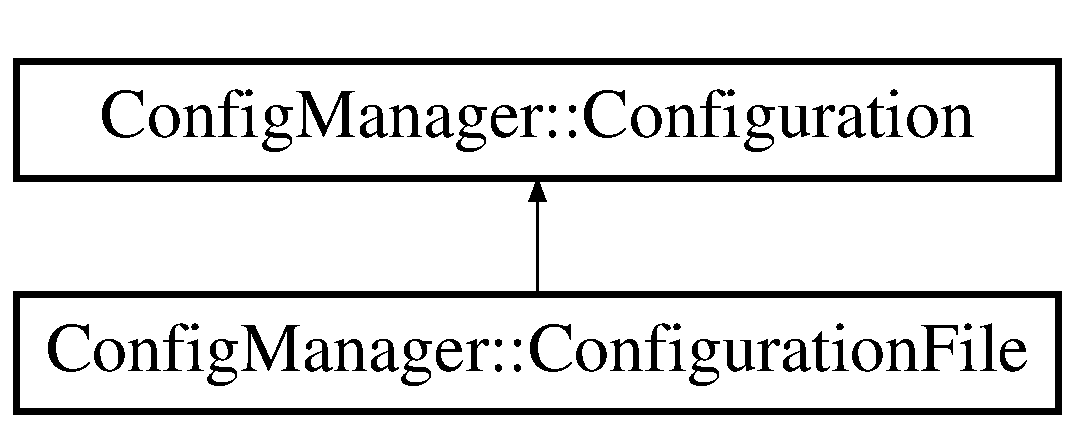
\includegraphics[height=2.000000cm]{class_config_manager_1_1_configuration}
\end{center}
\end{figure}
\subsection*{Public Member Functions}
\begin{DoxyCompactItemize}
\item 
\hyperlink{class_config_manager_1_1_configuration_aaaddf3eebe988ca26ecc4b9d85f798ea}{Configuration} ()
\item 
void \hyperlink{class_config_manager_1_1_configuration_a65fc8e2bef6af048e48438d7c385e834}{Open} (std\+::istream \&input\+\_\+stream)
\item 
void \hyperlink{class_config_manager_1_1_configuration_ac6c9646c929fd59c15d17beedf94ac74}{Check\+Strict} ()
\item 
void \hyperlink{class_config_manager_1_1_configuration_aa9922ac136da02f6588d60d731208d19}{Save} (std\+::ostream \&output\+\_\+stream, Output\+Method output\+\_\+method=Output\+Method\+::\+N\+O\+R\+M\+AL)
\item 
\hyperlink{class_config_manager_1_1_section}{Section} \hyperlink{class_config_manager_1_1_configuration_ac4d3be4b09060a773cffc45f47ad50a1}{Specify\+Section} (const std\+::string \&section\+\_\+name, Requirement requirement=Requirement\+::\+O\+P\+T\+I\+O\+N\+AL, const std\+::string \&comments=\char`\"{}\char`\"{})
\item 
\hyperlink{class_config_manager_1_1_section}{Section} \hyperlink{class_config_manager_1_1_configuration_a6e9bcd6f3a6d371996b86988fc54a730}{operator\mbox{[}$\,$\mbox{]}} (const std\+::string \&section\+\_\+name)
\item 
bool \hyperlink{class_config_manager_1_1_configuration_a15b0d2b3943be1672ca025034562b19c}{Is\+Loaded} () const 
\end{DoxyCompactItemize}


\subsection{Detailed Description}
Trida spravujici soubory s nastavenim. Vzhledem k tomu, ze soubory maji format \char`\"{}.\+ini\char`\"{} a jejich format tedy neni uplne specifikovany, uchovava tato trida puvodni retezcove hodnoty. Umoznuje pristupovat k sekcim a hodnotam daneho souboru pomoci metody Specify\+Section. V destruktoru jsou pripadne zmeny zapsany zpet do souboru. 

Definition at line 21 of file configuration.\+h.



\subsection{Constructor \& Destructor Documentation}
\index{Config\+Manager\+::\+Configuration@{Config\+Manager\+::\+Configuration}!Configuration@{Configuration}}
\index{Configuration@{Configuration}!Config\+Manager\+::\+Configuration@{Config\+Manager\+::\+Configuration}}
\subsubsection[{\texorpdfstring{Configuration()}{Configuration()}}]{\setlength{\rightskip}{0pt plus 5cm}Config\+Manager\+::\+Configuration\+::\+Configuration (
\begin{DoxyParamCaption}
{}
\end{DoxyParamCaption}
)}\hypertarget{class_config_manager_1_1_configuration_aaaddf3eebe988ca26ecc4b9d85f798ea}{}\label{class_config_manager_1_1_configuration_aaaddf3eebe988ca26ecc4b9d85f798ea}
Zakladni kontruktor. 

Definition at line 8 of file configuration.\+cpp.



\subsection{Member Function Documentation}
\index{Config\+Manager\+::\+Configuration@{Config\+Manager\+::\+Configuration}!Check\+Strict@{Check\+Strict}}
\index{Check\+Strict@{Check\+Strict}!Config\+Manager\+::\+Configuration@{Config\+Manager\+::\+Configuration}}
\subsubsection[{\texorpdfstring{Check\+Strict()}{CheckStrict()}}]{\setlength{\rightskip}{0pt plus 5cm}void Config\+Manager\+::\+Configuration\+::\+Check\+Strict (
\begin{DoxyParamCaption}
{}
\end{DoxyParamCaption}
)}\hypertarget{class_config_manager_1_1_configuration_ac6c9646c929fd59c15d17beedf94ac74}{}\label{class_config_manager_1_1_configuration_ac6c9646c929fd59c15d17beedf94ac74}
Metoda pro kontrolu, zda vstup odpovida jiz striktne specifikovanemu formatu. Muze vyhodit \hyperlink{class_config_manager_1_1_strict_exception}{Strict\+Exception} vyjimku. 

Definition at line 91 of file configuration.\+cpp.

\index{Config\+Manager\+::\+Configuration@{Config\+Manager\+::\+Configuration}!Is\+Loaded@{Is\+Loaded}}
\index{Is\+Loaded@{Is\+Loaded}!Config\+Manager\+::\+Configuration@{Config\+Manager\+::\+Configuration}}
\subsubsection[{\texorpdfstring{Is\+Loaded() const }{IsLoaded() const }}]{\setlength{\rightskip}{0pt plus 5cm}bool Config\+Manager\+::\+Configuration\+::\+Is\+Loaded (
\begin{DoxyParamCaption}
{}
\end{DoxyParamCaption}
) const}\hypertarget{class_config_manager_1_1_configuration_a15b0d2b3943be1672ca025034562b19c}{}\label{class_config_manager_1_1_configuration_a15b0d2b3943be1672ca025034562b19c}
Metoda vracejici, zda je v aktualne nactena nejaka konfigurace. 

Definition at line 206 of file configuration.\+cpp.

\index{Config\+Manager\+::\+Configuration@{Config\+Manager\+::\+Configuration}!Open@{Open}}
\index{Open@{Open}!Config\+Manager\+::\+Configuration@{Config\+Manager\+::\+Configuration}}
\subsubsection[{\texorpdfstring{Open(std\+::istream \&input\+\_\+stream)}{Open(std::istream &input_stream)}}]{\setlength{\rightskip}{0pt plus 5cm}void Config\+Manager\+::\+Configuration\+::\+Open (
\begin{DoxyParamCaption}
\item[{std\+::istream \&}]{input\+\_\+stream}
\end{DoxyParamCaption}
)}\hypertarget{class_config_manager_1_1_configuration_a65fc8e2bef6af048e48438d7c385e834}{}\label{class_config_manager_1_1_configuration_a65fc8e2bef6af048e48438d7c385e834}
Metoda pro nastaveni vstupniho streamu. Muze vyhodit \hyperlink{class_config_manager_1_1_malformed_input_exception}{Malformed\+Input\+Exception}, \hyperlink{class_config_manager_1_1_io_exception}{Io\+Exception}, \hyperlink{class_config_manager_1_1_wrong_format_exception}{Wrong\+Format\+Exception}, \hyperlink{class_config_manager_1_1_mandatory_missing_exception}{Mandatory\+Missing\+Exception} vyjimky. 
\begin{DoxyParams}{Parameters}
{\em input\+\_\+stream} & Vstupni istream. \\
\hline
\end{DoxyParams}


Definition at line 13 of file configuration.\+cpp.

\index{Config\+Manager\+::\+Configuration@{Config\+Manager\+::\+Configuration}!operator\mbox{[}$\,$\mbox{]}@{operator[]}}
\index{operator\mbox{[}$\,$\mbox{]}@{operator[]}!Config\+Manager\+::\+Configuration@{Config\+Manager\+::\+Configuration}}
\subsubsection[{\texorpdfstring{operator[](const std\+::string \&section\+\_\+name)}{operator[](const std::string &section_name)}}]{\setlength{\rightskip}{0pt plus 5cm}{\bf Section} Config\+Manager\+::\+Configuration\+::operator\mbox{[}$\,$\mbox{]} (
\begin{DoxyParamCaption}
\item[{const std\+::string \&}]{section\+\_\+name}
\end{DoxyParamCaption}
)}\hypertarget{class_config_manager_1_1_configuration_a6e9bcd6f3a6d371996b86988fc54a730}{}\label{class_config_manager_1_1_configuration_a6e9bcd6f3a6d371996b86988fc54a730}
Metoda zpristupnujici dalsi sekci. Lze pouzit nezavisle na zavolani Specify\+Section. 
\begin{DoxyParams}{Parameters}
{\em section\+\_\+name} & Jmeno sekce. \\
\hline
\end{DoxyParams}


Definition at line 194 of file configuration.\+cpp.

\index{Config\+Manager\+::\+Configuration@{Config\+Manager\+::\+Configuration}!Save@{Save}}
\index{Save@{Save}!Config\+Manager\+::\+Configuration@{Config\+Manager\+::\+Configuration}}
\subsubsection[{\texorpdfstring{Save(std\+::ostream \&output\+\_\+stream, Output\+Method output\+\_\+method=\+Output\+Method\+::\+N\+O\+R\+M\+A\+L)}{Save(std::ostream &output_stream, OutputMethod output_method=OutputMethod::NORMAL)}}]{\setlength{\rightskip}{0pt plus 5cm}void Config\+Manager\+::\+Configuration\+::\+Save (
\begin{DoxyParamCaption}
\item[{std\+::ostream \&}]{output\+\_\+stream, }
\item[{Output\+Method}]{output\+\_\+method = {\ttfamily OutputMethod\+:\+:NORMAL}}
\end{DoxyParamCaption}
)}\hypertarget{class_config_manager_1_1_configuration_aa9922ac136da02f6588d60d731208d19}{}\label{class_config_manager_1_1_configuration_aa9922ac136da02f6588d60d731208d19}
Metoda vynucijici zapis zmenenych voleb na disk. Muze vyhodit \hyperlink{class_config_manager_1_1_io_exception}{Io\+Exception} vyjimku (v p�ipad� selh�n� otev�en� souboru pro z�pis). 
\begin{DoxyParams}{Parameters}
{\em output\+\_\+method} & Volba zapisu prednastavenych hodnot. \\
\hline
\end{DoxyParams}


Definition at line 120 of file configuration.\+cpp.

\index{Config\+Manager\+::\+Configuration@{Config\+Manager\+::\+Configuration}!Specify\+Section@{Specify\+Section}}
\index{Specify\+Section@{Specify\+Section}!Config\+Manager\+::\+Configuration@{Config\+Manager\+::\+Configuration}}
\subsubsection[{\texorpdfstring{Specify\+Section(const std\+::string \&section\+\_\+name, Requirement requirement=\+Requirement\+::\+O\+P\+T\+I\+O\+N\+A\+L, const std\+::string \&comments="""")}{SpecifySection(const std::string &section_name, Requirement requirement=Requirement::OPTIONAL, const std::string &comments="")}}]{\setlength{\rightskip}{0pt plus 5cm}{\bf Section} Config\+Manager\+::\+Configuration\+::\+Specify\+Section (
\begin{DoxyParamCaption}
\item[{const std\+::string \&}]{section\+\_\+name, }
\item[{Requirement}]{requirement = {\ttfamily Requirement\+:\+:OPTIONAL}, }
\item[{const std\+::string \&}]{comments = {\ttfamily \char`\"{}\char`\"{}}}
\end{DoxyParamCaption}
)}\hypertarget{class_config_manager_1_1_configuration_ac4d3be4b09060a773cffc45f47ad50a1}{}\label{class_config_manager_1_1_configuration_ac4d3be4b09060a773cffc45f47ad50a1}
Metoda specifikujici dalsi sekci. Muze vyhodit \hyperlink{class_config_manager_1_1_mandatory_missing_exception}{Mandatory\+Missing\+Exception} vyjimku. 
\begin{DoxyParams}{Parameters}
{\em section\+\_\+name} & Jmeno sekce. \\
\hline
{\em requirement} & Povinnost dane sekce. \\
\hline
{\em comments} & Komentare k dane sekci. \\
\hline
\end{DoxyParams}


Definition at line 178 of file configuration.\+cpp.



The documentation for this class was generated from the following files\+:\begin{DoxyCompactItemize}
\item 
E\+:/\+I\+N\+F\+O\+R\+M\+A\+T\+I\+K\+A/doporucene\+Postupy/uloha4/repos/src/\+Config\+Manager/configuration.\+h\item 
E\+:/\+I\+N\+F\+O\+R\+M\+A\+T\+I\+K\+A/doporucene\+Postupy/uloha4/repos/src/\+Config\+Manager/configuration.\+cpp\end{DoxyCompactItemize}

\hypertarget{class_config_manager_1_1_configuration_exception}{}\section{Config\+Manager\+:\+:Configuration\+Exception Class Reference}
\label{class_config_manager_1_1_configuration_exception}\index{Config\+Manager\+::\+Configuration\+Exception@{Config\+Manager\+::\+Configuration\+Exception}}
Inheritance diagram for Config\+Manager\+:\+:Configuration\+Exception\+:\begin{figure}[H]
\begin{center}
\leavevmode
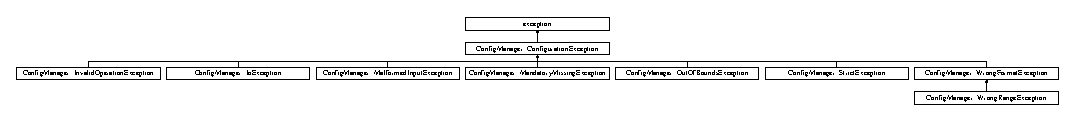
\includegraphics[height=1.172161cm]{class_config_manager_1_1_configuration_exception}
\end{center}
\end{figure}
\subsection*{Public Member Functions}
\begin{DoxyCompactItemize}
\item 
{\bfseries Configuration\+Exception} (const char $\ast$message)\hypertarget{class_config_manager_1_1_configuration_exception_a7ab971ae1aa991968064f7414f233afd}{}\label{class_config_manager_1_1_configuration_exception_a7ab971ae1aa991968064f7414f233afd}

\item 
const char $\ast$ {\bfseries what} () const  override  throw ()\hypertarget{class_config_manager_1_1_configuration_exception_a2896099b9b4ced84a7359136105e9937}{}\label{class_config_manager_1_1_configuration_exception_a2896099b9b4ced84a7359136105e9937}

\end{DoxyCompactItemize}


\subsection{Detailed Description}


Definition at line 6 of file exceptions.\+h.



The documentation for this class was generated from the following file\+:\begin{DoxyCompactItemize}
\item 
E\+:/\+I\+N\+F\+O\+R\+M\+A\+T\+I\+K\+A/doporucene\+Postupy/uloha4/repos/src/\+Config\+Manager/exceptions.\+h\end{DoxyCompactItemize}

\hypertarget{class_config_manager_1_1_configuration_file}{}\section{Config\+Manager\+:\+:Configuration\+File Class Reference}
\label{class_config_manager_1_1_configuration_file}\index{Config\+Manager\+::\+Configuration\+File@{Config\+Manager\+::\+Configuration\+File}}
Inheritance diagram for Config\+Manager\+:\+:Configuration\+File\+:\begin{figure}[H]
\begin{center}
\leavevmode
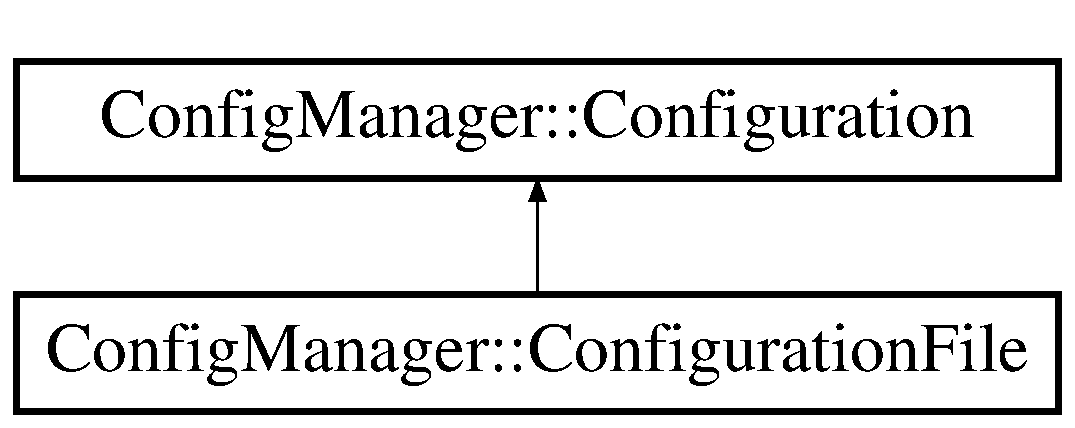
\includegraphics[height=2.000000cm]{class_config_manager_1_1_configuration_file}
\end{center}
\end{figure}
\subsection*{Public Member Functions}
\begin{DoxyCompactItemize}
\item 
\hyperlink{class_config_manager_1_1_configuration_file_a07d5355e097215f22a31f8e3e1d73aae}{Configuration\+File} (std\+::string filename, Input\+File\+Policy policy=Input\+File\+Policy\+::\+N\+O\+NE)
\item 
\hyperlink{class_config_manager_1_1_configuration_file_ab58c1860cb0d3b502f674975000736a5}{$\sim$\+Configuration\+File} ()
\end{DoxyCompactItemize}


\subsection{Detailed Description}


Definition at line 78 of file configuration.\+h.



\subsection{Constructor \& Destructor Documentation}
\index{Config\+Manager\+::\+Configuration\+File@{Config\+Manager\+::\+Configuration\+File}!Configuration\+File@{Configuration\+File}}
\index{Configuration\+File@{Configuration\+File}!Config\+Manager\+::\+Configuration\+File@{Config\+Manager\+::\+Configuration\+File}}
\subsubsection[{\texorpdfstring{Configuration\+File(std\+::string filename, Input\+File\+Policy policy=\+Input\+File\+Policy\+::\+N\+O\+N\+E)}{ConfigurationFile(std::string filename, InputFilePolicy policy=InputFilePolicy::NONE)}}]{\setlength{\rightskip}{0pt plus 5cm}Config\+Manager\+::\+Configuration\+File\+::\+Configuration\+File (
\begin{DoxyParamCaption}
\item[{std\+::string}]{filename, }
\item[{Input\+File\+Policy}]{policy = {\ttfamily InputFilePolicy\+:\+:NONE}}
\end{DoxyParamCaption}
)}\hypertarget{class_config_manager_1_1_configuration_file_a07d5355e097215f22a31f8e3e1d73aae}{}\label{class_config_manager_1_1_configuration_file_a07d5355e097215f22a31f8e3e1d73aae}
Konstruktor nacitajici nastaveni ze zvoleneho souboru. Muze vyhodit \hyperlink{class_config_manager_1_1_malformed_input_exception}{Malformed\+Input\+Exception}, \hyperlink{class_config_manager_1_1_io_exception}{Io\+Exception} vyjimky. 
\begin{DoxyParams}{Parameters}
{\em filename} & Jmeno souboru. (Ocekavany format \char`\"{}.\+ini\char`\"{}) \\
\hline
{\em policy} & Spefikuje pristup k vstupnimu souboru (relaxed/strict). \\
\hline
\end{DoxyParams}


Definition at line 213 of file configuration.\+cpp.

\index{Config\+Manager\+::\+Configuration\+File@{Config\+Manager\+::\+Configuration\+File}!````~Configuration\+File@{$\sim$\+Configuration\+File}}
\index{````~Configuration\+File@{$\sim$\+Configuration\+File}!Config\+Manager\+::\+Configuration\+File@{Config\+Manager\+::\+Configuration\+File}}
\subsubsection[{\texorpdfstring{$\sim$\+Configuration\+File()}{~ConfigurationFile()}}]{\setlength{\rightskip}{0pt plus 5cm}Config\+Manager\+::\+Configuration\+File\+::$\sim$\+Configuration\+File (
\begin{DoxyParamCaption}
{}
\end{DoxyParamCaption}
)}\hypertarget{class_config_manager_1_1_configuration_file_ab58c1860cb0d3b502f674975000736a5}{}\label{class_config_manager_1_1_configuration_file_ab58c1860cb0d3b502f674975000736a5}
Zakladni dektruktor. Vsechny zmenene volby se program pokusi ulozit na urcene misto (soubor/istream). Muze selhat obdobne jako \hyperlink{class_config_manager_1_1_configuration_aa9922ac136da02f6588d60d731208d19}{Save()}, ale nevyhazuje vyjimky (jelikoz vyjimka z destruktoru by zpusobila pad programu, pokud jiz doslo k jine vyjimce). 

Definition at line 220 of file configuration.\+cpp.



The documentation for this class was generated from the following files\+:\begin{DoxyCompactItemize}
\item 
src/\+Config\+Manager/configuration.\+h\item 
src/\+Config\+Manager/configuration.\+cpp\end{DoxyCompactItemize}

\hypertarget{class_configuration_test_suite}{}\section{Configuration\+Test\+Suite Class Reference}
\label{class_configuration_test_suite}\index{Configuration\+Test\+Suite@{Configuration\+Test\+Suite}}
Inheritance diagram for Configuration\+Test\+Suite\+:\begin{figure}[H]
\begin{center}
\leavevmode
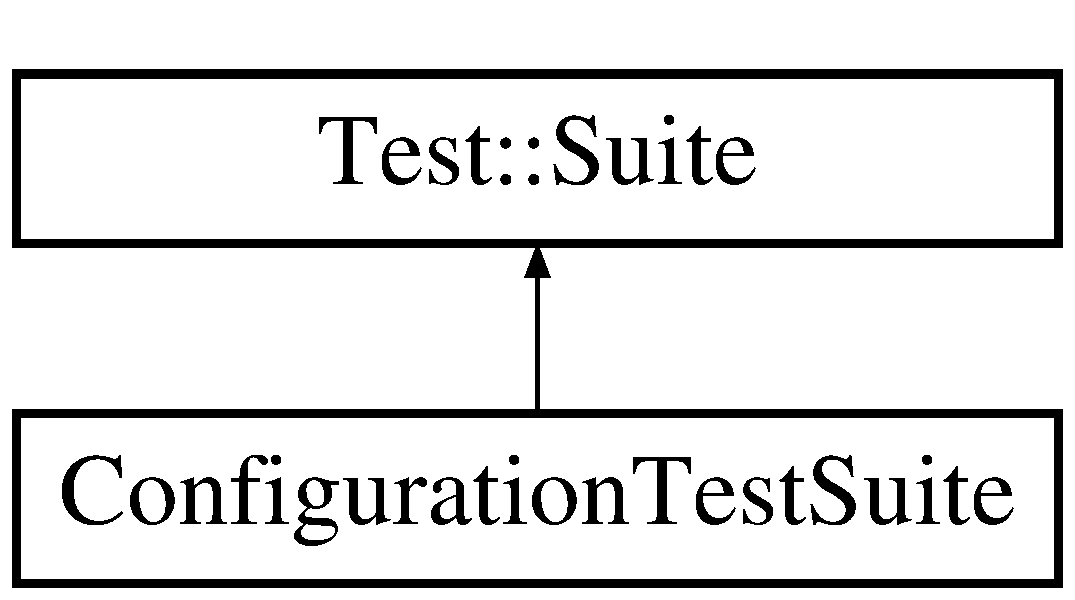
\includegraphics[height=2.000000cm]{class_configuration_test_suite}
\end{center}
\end{figure}
\subsection*{Additional Inherited Members}


\subsection{Detailed Description}


Definition at line 11 of file tests.\+h.



The documentation for this class was generated from the following files\+:\begin{DoxyCompactItemize}
\item 
tests/tests.\+h\item 
tests/tests.\+cpp\end{DoxyCompactItemize}

\hypertarget{struct_test_1_1_suite_1_1_do_run}{}\section{Test\+:\+:Suite\+:\+:Do\+Run Struct Reference}
\label{struct_test_1_1_suite_1_1_do_run}\index{Test\+::\+Suite\+::\+Do\+Run@{Test\+::\+Suite\+::\+Do\+Run}}
\subsection*{Public Member Functions}
\begin{DoxyCompactItemize}
\item 
{\bfseries Do\+Run} (\hyperlink{class_test_1_1_output}{Output} $\ast$output, bool cont)\hypertarget{struct_test_1_1_suite_1_1_do_run_ae4fa291dd6956a7aa1507bde2d2596f7}{}\label{struct_test_1_1_suite_1_1_do_run_ae4fa291dd6956a7aa1507bde2d2596f7}

\item 
void {\bfseries operator()} (\hyperlink{class_test_1_1_suite}{Suite} $\ast$suite)\hypertarget{struct_test_1_1_suite_1_1_do_run_ae1196082bc99fed5dbf7c31608950fec}{}\label{struct_test_1_1_suite_1_1_do_run_ae1196082bc99fed5dbf7c31608950fec}

\end{DoxyCompactItemize}
\subsection*{Public Attributes}
\begin{DoxyCompactItemize}
\item 
bool {\bfseries \+\_\+continue}\hypertarget{struct_test_1_1_suite_1_1_do_run_aec0de4a2fe5c782f036f26b82a4eeba4}{}\label{struct_test_1_1_suite_1_1_do_run_aec0de4a2fe5c782f036f26b82a4eeba4}

\item 
\hyperlink{class_test_1_1_output}{Output} $\ast$ {\bfseries \+\_\+output}\hypertarget{struct_test_1_1_suite_1_1_do_run_aeff5d2f886719ca02ff7cbab9548d8ad}{}\label{struct_test_1_1_suite_1_1_do_run_aeff5d2f886719ca02ff7cbab9548d8ad}

\end{DoxyCompactItemize}


\subsection{Detailed Description}


Definition at line 193 of file suite.\+cpp.



The documentation for this struct was generated from the following file\+:\begin{DoxyCompactItemize}
\item 
lib/cpptest-\/1.\+1.\+2/src/suite.\+cpp\end{DoxyCompactItemize}

\hypertarget{class_config_manager_1_1_enum_specifier}{}\section{Config\+Manager\+:\+:Enum\+Specifier$<$ T\+Result $>$ Class Template Reference}
\label{class_config_manager_1_1_enum_specifier}\index{Config\+Manager\+::\+Enum\+Specifier$<$ T\+Result $>$@{Config\+Manager\+::\+Enum\+Specifier$<$ T\+Result $>$}}


{\ttfamily \#include $<$typespecifiers.\+h$>$}

\subsection*{Public Types}
\begin{DoxyCompactItemize}
\item 
typedef T\+Result \hyperlink{class_config_manager_1_1_enum_specifier_a05ef7c4dcc62170fb20c2626d65c73ab}{Value\+Type}
\end{DoxyCompactItemize}
\subsection*{Public Member Functions}
\begin{DoxyCompactItemize}
\item 
\hyperlink{class_config_manager_1_1_enum_specifier_a70c4b632b975b383b5c7ea087e229425}{Enum\+Specifier} (const std\+::map$<$ std\+::string, \hyperlink{class_config_manager_1_1_enum_specifier_a05ef7c4dcc62170fb20c2626d65c73ab}{Value\+Type} $>$ \&value\+\_\+mapping)
\item 
const \hyperlink{class_config_manager_1_1_enum_specifier_a05ef7c4dcc62170fb20c2626d65c73ab}{Value\+Type} \& \hyperlink{class_config_manager_1_1_enum_specifier_a12977b0c8cb9294a4722c6ba74d08788}{From\+String} (const std\+::string \&data)
\item 
const std\+::string \& \hyperlink{class_config_manager_1_1_enum_specifier_a619291d6ec0416be07139767429ba412}{To\+String} (const \hyperlink{class_config_manager_1_1_enum_specifier_a05ef7c4dcc62170fb20c2626d65c73ab}{Value\+Type} \&value)
\end{DoxyCompactItemize}


\subsection{Detailed Description}
\subsubsection*{template$<$typename T\+Result$>$\\*
class Config\+Manager\+::\+Enum\+Specifier$<$ T\+Result $>$}

Trida realizujici prevod z textu do typu vyctovy typ a zpet. Presny vyctovy typ je specifikovan parametrem sablony. 

Definition at line 200 of file typespecifiers.\+h.



\subsection{Member Typedef Documentation}
\index{Config\+Manager\+::\+Enum\+Specifier@{Config\+Manager\+::\+Enum\+Specifier}!Value\+Type@{Value\+Type}}
\index{Value\+Type@{Value\+Type}!Config\+Manager\+::\+Enum\+Specifier@{Config\+Manager\+::\+Enum\+Specifier}}
\subsubsection[{\texorpdfstring{Value\+Type}{ValueType}}]{\setlength{\rightskip}{0pt plus 5cm}template$<$typename T\+Result $>$ typedef T\+Result {\bf Config\+Manager\+::\+Enum\+Specifier}$<$ T\+Result $>$\+::{\bf Value\+Type}}\hypertarget{class_config_manager_1_1_enum_specifier_a05ef7c4dcc62170fb20c2626d65c73ab}{}\label{class_config_manager_1_1_enum_specifier_a05ef7c4dcc62170fb20c2626d65c73ab}




Tato definice typu urcuje navratovy typ. 

Definition at line 206 of file typespecifiers.\+h.



\subsection{Constructor \& Destructor Documentation}
\index{Config\+Manager\+::\+Enum\+Specifier@{Config\+Manager\+::\+Enum\+Specifier}!Enum\+Specifier@{Enum\+Specifier}}
\index{Enum\+Specifier@{Enum\+Specifier}!Config\+Manager\+::\+Enum\+Specifier@{Config\+Manager\+::\+Enum\+Specifier}}
\subsubsection[{\texorpdfstring{Enum\+Specifier(const std\+::map$<$ std\+::string, Value\+Type $>$ \&value\+\_\+mapping)}{EnumSpecifier(const std::map< std::string, ValueType > &value_mapping)}}]{\setlength{\rightskip}{0pt plus 5cm}template$<$typename T\+Result $>$ {\bf Config\+Manager\+::\+Enum\+Specifier}$<$ T\+Result $>$\+::{\bf Enum\+Specifier} (
\begin{DoxyParamCaption}
\item[{const std\+::map$<$ std\+::string, {\bf Value\+Type} $>$ \&}]{value\+\_\+mapping}
\end{DoxyParamCaption}
)}\hypertarget{class_config_manager_1_1_enum_specifier_a70c4b632b975b383b5c7ea087e229425}{}\label{class_config_manager_1_1_enum_specifier_a70c4b632b975b383b5c7ea087e229425}
Zaladni konstruktor. Meze vyctoveho typu jsou jiz specifikovany. 

Definition at line 291 of file typespecifiers.\+h.



\subsection{Member Function Documentation}
\index{Config\+Manager\+::\+Enum\+Specifier@{Config\+Manager\+::\+Enum\+Specifier}!From\+String@{From\+String}}
\index{From\+String@{From\+String}!Config\+Manager\+::\+Enum\+Specifier@{Config\+Manager\+::\+Enum\+Specifier}}
\subsubsection[{\texorpdfstring{From\+String(const std\+::string \&data)}{FromString(const std::string &data)}}]{\setlength{\rightskip}{0pt plus 5cm}template$<$typename T\+Result $>$ auto {\bf Config\+Manager\+::\+Enum\+Specifier}$<$ T\+Result $>$\+::From\+String (
\begin{DoxyParamCaption}
\item[{const std\+::string \&}]{data}
\end{DoxyParamCaption}
)}\hypertarget{class_config_manager_1_1_enum_specifier_a12977b0c8cb9294a4722c6ba74d08788}{}\label{class_config_manager_1_1_enum_specifier_a12977b0c8cb9294a4722c6ba74d08788}




Metoda prevadejici text na vyslednou hodnotu. Muze vyhodit \hyperlink{class_config_manager_1_1_wrong_format_exception}{Wrong\+Format\+Exception} vyjimku. 
\begin{DoxyParams}{Parameters}
{\em data} & Vstupni data. \\
\hline
\end{DoxyParams}


Definition at line 297 of file typespecifiers.\+h.

\index{Config\+Manager\+::\+Enum\+Specifier@{Config\+Manager\+::\+Enum\+Specifier}!To\+String@{To\+String}}
\index{To\+String@{To\+String}!Config\+Manager\+::\+Enum\+Specifier@{Config\+Manager\+::\+Enum\+Specifier}}
\subsubsection[{\texorpdfstring{To\+String(const Value\+Type \&value)}{ToString(const ValueType &value)}}]{\setlength{\rightskip}{0pt plus 5cm}template$<$typename T\+Result $>$ const std\+::string \& {\bf Config\+Manager\+::\+Enum\+Specifier}$<$ T\+Result $>$\+::To\+String (
\begin{DoxyParamCaption}
\item[{const {\bf Value\+Type} \&}]{value}
\end{DoxyParamCaption}
)}\hypertarget{class_config_manager_1_1_enum_specifier_a619291d6ec0416be07139767429ba412}{}\label{class_config_manager_1_1_enum_specifier_a619291d6ec0416be07139767429ba412}






Definition at line 306 of file typespecifiers.\+h.



The documentation for this class was generated from the following file\+:\begin{DoxyCompactItemize}
\item 
E\+:/\+I\+N\+F\+O\+R\+M\+A\+T\+I\+K\+A/doporucene\+Postupy/uloha4/repos/src/\+Config\+Manager/typespecifiers.\+h\end{DoxyCompactItemize}

\hypertarget{struct_test_1_1_suite_1_1_exec_tests}{}\section{Test\+:\+:Suite\+:\+:Exec\+Tests Struct Reference}
\label{struct_test_1_1_suite_1_1_exec_tests}\index{Test\+::\+Suite\+::\+Exec\+Tests@{Test\+::\+Suite\+::\+Exec\+Tests}}
\subsection*{Public Member Functions}
\begin{DoxyCompactItemize}
\item 
{\bfseries Exec\+Tests} (\hyperlink{class_test_1_1_suite}{Suite} \&s)\hypertarget{struct_test_1_1_suite_1_1_exec_tests_a49e123e603aa95feae5e83e1754c4676}{}\label{struct_test_1_1_suite_1_1_exec_tests_a49e123e603aa95feae5e83e1754c4676}

\item 
void {\bfseries operator()} (Data \&data)\hypertarget{struct_test_1_1_suite_1_1_exec_tests_acfc10f09bd6c369114202742d098ff10}{}\label{struct_test_1_1_suite_1_1_exec_tests_acfc10f09bd6c369114202742d098ff10}

\end{DoxyCompactItemize}
\subsection*{Public Attributes}
\begin{DoxyCompactItemize}
\item 
\hyperlink{class_test_1_1_suite}{Suite} \& {\bfseries \+\_\+suite}\hypertarget{struct_test_1_1_suite_1_1_exec_tests_ab0bf7c14d635c9c2da8546c6a57b05f3}{}\label{struct_test_1_1_suite_1_1_exec_tests_ab0bf7c14d635c9c2da8546c6a57b05f3}

\end{DoxyCompactItemize}


\subsection{Detailed Description}


Definition at line 162 of file suite.\+cpp.



The documentation for this struct was generated from the following file\+:\begin{DoxyCompactItemize}
\item 
lib/cpptest-\/1.\+1.\+2/src/suite.\+cpp\end{DoxyCompactItemize}

\hypertarget{class_fail_test_suite}{}\section{Fail\+Test\+Suite Class Reference}
\label{class_fail_test_suite}\index{Fail\+Test\+Suite@{Fail\+Test\+Suite}}
Inheritance diagram for Fail\+Test\+Suite\+:\begin{figure}[H]
\begin{center}
\leavevmode
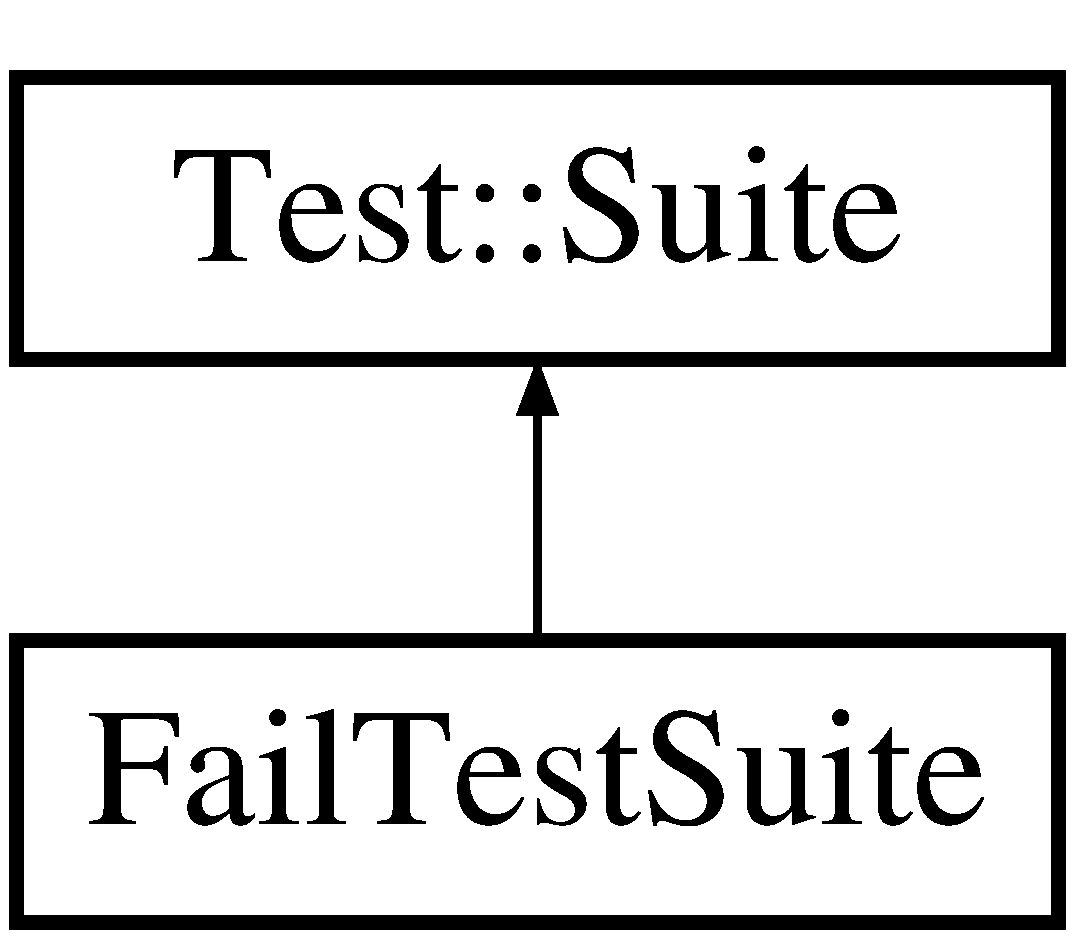
\includegraphics[height=2.000000cm]{class_fail_test_suite}
\end{center}
\end{figure}
\subsection*{Additional Inherited Members}


\subsection{Detailed Description}


Definition at line 45 of file mytest.\+cpp.



The documentation for this class was generated from the following file\+:\begin{DoxyCompactItemize}
\item 
lib/cpptest-\/1.\+1.\+2/test/mytest.\+cpp\end{DoxyCompactItemize}

\hypertarget{class_config_manager_1_1_float_specifier}{}\section{Config\+Manager\+:\+:Float\+Specifier Class Reference}
\label{class_config_manager_1_1_float_specifier}\index{Config\+Manager\+::\+Float\+Specifier@{Config\+Manager\+::\+Float\+Specifier}}


{\ttfamily \#include $<$typespecifiers.\+h$>$}

Inheritance diagram for Config\+Manager\+:\+:Float\+Specifier\+:\begin{figure}[H]
\begin{center}
\leavevmode
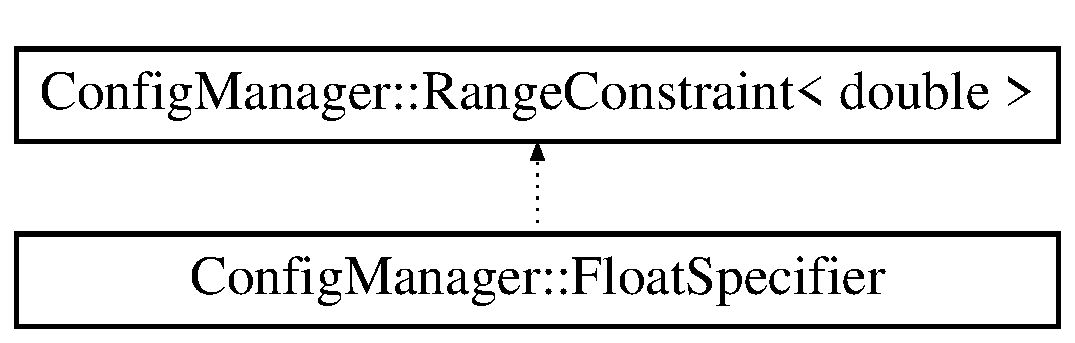
\includegraphics[height=2.000000cm]{class_config_manager_1_1_float_specifier}
\end{center}
\end{figure}
\subsection*{Public Types}
\begin{DoxyCompactItemize}
\item 
typedef double \hyperlink{class_config_manager_1_1_float_specifier_aa31aedae65d89c1c14d9b0aa6fbe697b}{Value\+Type}
\end{DoxyCompactItemize}
\subsection*{Public Member Functions}
\begin{DoxyCompactItemize}
\item 
\hyperlink{class_config_manager_1_1_float_specifier_aeaefabf4a53b45d70575e50a16ecff95}{Float\+Specifier} ()
\item 
\hyperlink{class_config_manager_1_1_float_specifier_a841c065d50fdedccac00822b4bc36e65}{Float\+Specifier} (double range\+\_\+start, double range\+\_\+end)
\item 
\hyperlink{class_config_manager_1_1_float_specifier_aa31aedae65d89c1c14d9b0aa6fbe697b}{Value\+Type} \hyperlink{class_config_manager_1_1_float_specifier_a557eaa40035aa402e0f4cd24e3ed5e17}{From\+String} (const std\+::string \&data)
\item 
std\+::string \hyperlink{class_config_manager_1_1_float_specifier_a161a99d1f205292ce0b4a17bb0a8daeb}{To\+String} (\hyperlink{class_config_manager_1_1_float_specifier_aa31aedae65d89c1c14d9b0aa6fbe697b}{Value\+Type} value)
\end{DoxyCompactItemize}


\subsection{Detailed Description}
Trida realizujici prevod z textu do typu float a zpet. 

Definition at line 153 of file typespecifiers.\+h.



\subsection{Member Typedef Documentation}
\index{Config\+Manager\+::\+Float\+Specifier@{Config\+Manager\+::\+Float\+Specifier}!Value\+Type@{Value\+Type}}
\index{Value\+Type@{Value\+Type}!Config\+Manager\+::\+Float\+Specifier@{Config\+Manager\+::\+Float\+Specifier}}
\subsubsection[{\texorpdfstring{Value\+Type}{ValueType}}]{\setlength{\rightskip}{0pt plus 5cm}typedef double {\bf Config\+Manager\+::\+Float\+Specifier\+::\+Value\+Type}}\hypertarget{class_config_manager_1_1_float_specifier_aa31aedae65d89c1c14d9b0aa6fbe697b}{}\label{class_config_manager_1_1_float_specifier_aa31aedae65d89c1c14d9b0aa6fbe697b}




Tato definice typu urcuje navratovy typ. 

Definition at line 159 of file typespecifiers.\+h.



\subsection{Constructor \& Destructor Documentation}
\index{Config\+Manager\+::\+Float\+Specifier@{Config\+Manager\+::\+Float\+Specifier}!Float\+Specifier@{Float\+Specifier}}
\index{Float\+Specifier@{Float\+Specifier}!Config\+Manager\+::\+Float\+Specifier@{Config\+Manager\+::\+Float\+Specifier}}
\subsubsection[{\texorpdfstring{Float\+Specifier()}{FloatSpecifier()}}]{\setlength{\rightskip}{0pt plus 5cm}Config\+Manager\+::\+Float\+Specifier\+::\+Float\+Specifier (
\begin{DoxyParamCaption}
{}
\end{DoxyParamCaption}
)}\hypertarget{class_config_manager_1_1_float_specifier_aeaefabf4a53b45d70575e50a16ecff95}{}\label{class_config_manager_1_1_float_specifier_aeaefabf4a53b45d70575e50a16ecff95}




Konstruktor ktery neklade omezeni mezeni na rozsah hodnot. Rozsah hodnot je potom dan rozsahem zvoleneho typu. 

Definition at line 162 of file typespecifiers.\+cpp.

\index{Config\+Manager\+::\+Float\+Specifier@{Config\+Manager\+::\+Float\+Specifier}!Float\+Specifier@{Float\+Specifier}}
\index{Float\+Specifier@{Float\+Specifier}!Config\+Manager\+::\+Float\+Specifier@{Config\+Manager\+::\+Float\+Specifier}}
\subsubsection[{\texorpdfstring{Float\+Specifier(double range\+\_\+start, double range\+\_\+end)}{FloatSpecifier(double range_start, double range_end)}}]{\setlength{\rightskip}{0pt plus 5cm}Config\+Manager\+::\+Float\+Specifier\+::\+Float\+Specifier (
\begin{DoxyParamCaption}
\item[{double}]{range\+\_\+start, }
\item[{double}]{range\+\_\+end}
\end{DoxyParamCaption}
)}\hypertarget{class_config_manager_1_1_float_specifier_a841c065d50fdedccac00822b4bc36e65}{}\label{class_config_manager_1_1_float_specifier_a841c065d50fdedccac00822b4bc36e65}
Konstruktor se specifikovanym rozsahem pro parametr. 
\begin{DoxyParams}{Parameters}
{\em range\+\_\+start} & Spodni meze rozsahu. \\
\hline
{\em range\+\_\+end} & Horni meze rozsahu. \\
\hline
\end{DoxyParams}


Definition at line 166 of file typespecifiers.\+cpp.



\subsection{Member Function Documentation}
\index{Config\+Manager\+::\+Float\+Specifier@{Config\+Manager\+::\+Float\+Specifier}!From\+String@{From\+String}}
\index{From\+String@{From\+String}!Config\+Manager\+::\+Float\+Specifier@{Config\+Manager\+::\+Float\+Specifier}}
\subsubsection[{\texorpdfstring{From\+String(const std\+::string \&data)}{FromString(const std::string &data)}}]{\setlength{\rightskip}{0pt plus 5cm}{\bf Float\+Specifier\+::\+Value\+Type} Config\+Manager\+::\+Float\+Specifier\+::\+From\+String (
\begin{DoxyParamCaption}
\item[{const std\+::string \&}]{data}
\end{DoxyParamCaption}
)}\hypertarget{class_config_manager_1_1_float_specifier_a557eaa40035aa402e0f4cd24e3ed5e17}{}\label{class_config_manager_1_1_float_specifier_a557eaa40035aa402e0f4cd24e3ed5e17}




Metoda prevadejici text na vyslednou hodnotu. Muze vyhodit \hyperlink{class_config_manager_1_1_wrong_format_exception}{Wrong\+Format\+Exception} vyjimku. 
\begin{DoxyParams}{Parameters}
{\em data} & Vstupni data. \\
\hline
\end{DoxyParams}


Definition at line 171 of file typespecifiers.\+cpp.

\index{Config\+Manager\+::\+Float\+Specifier@{Config\+Manager\+::\+Float\+Specifier}!To\+String@{To\+String}}
\index{To\+String@{To\+String}!Config\+Manager\+::\+Float\+Specifier@{Config\+Manager\+::\+Float\+Specifier}}
\subsubsection[{\texorpdfstring{To\+String(\+Value\+Type value)}{ToString(ValueType value)}}]{\setlength{\rightskip}{0pt plus 5cm}std\+::string Config\+Manager\+::\+Float\+Specifier\+::\+To\+String (
\begin{DoxyParamCaption}
\item[{{\bf Value\+Type}}]{value}
\end{DoxyParamCaption}
)}\hypertarget{class_config_manager_1_1_float_specifier_a161a99d1f205292ce0b4a17bb0a8daeb}{}\label{class_config_manager_1_1_float_specifier_a161a99d1f205292ce0b4a17bb0a8daeb}






Definition at line 185 of file typespecifiers.\+cpp.



The documentation for this class was generated from the following files\+:\begin{DoxyCompactItemize}
\item 
src/\+Config\+Manager/typespecifiers.\+h\item 
src/\+Config\+Manager/typespecifiers.\+cpp\end{DoxyCompactItemize}

\hypertarget{class_test_1_1_html_output}{}\section{Test\+:\+:Html\+Output Class Reference}
\label{class_test_1_1_html_output}\index{Test\+::\+Html\+Output@{Test\+::\+Html\+Output}}


H\+T\+ML output.  




{\ttfamily \#include $<$cpptest-\/htmloutput.\+h$>$}

Inheritance diagram for Test\+:\+:Html\+Output\+:\begin{figure}[H]
\begin{center}
\leavevmode
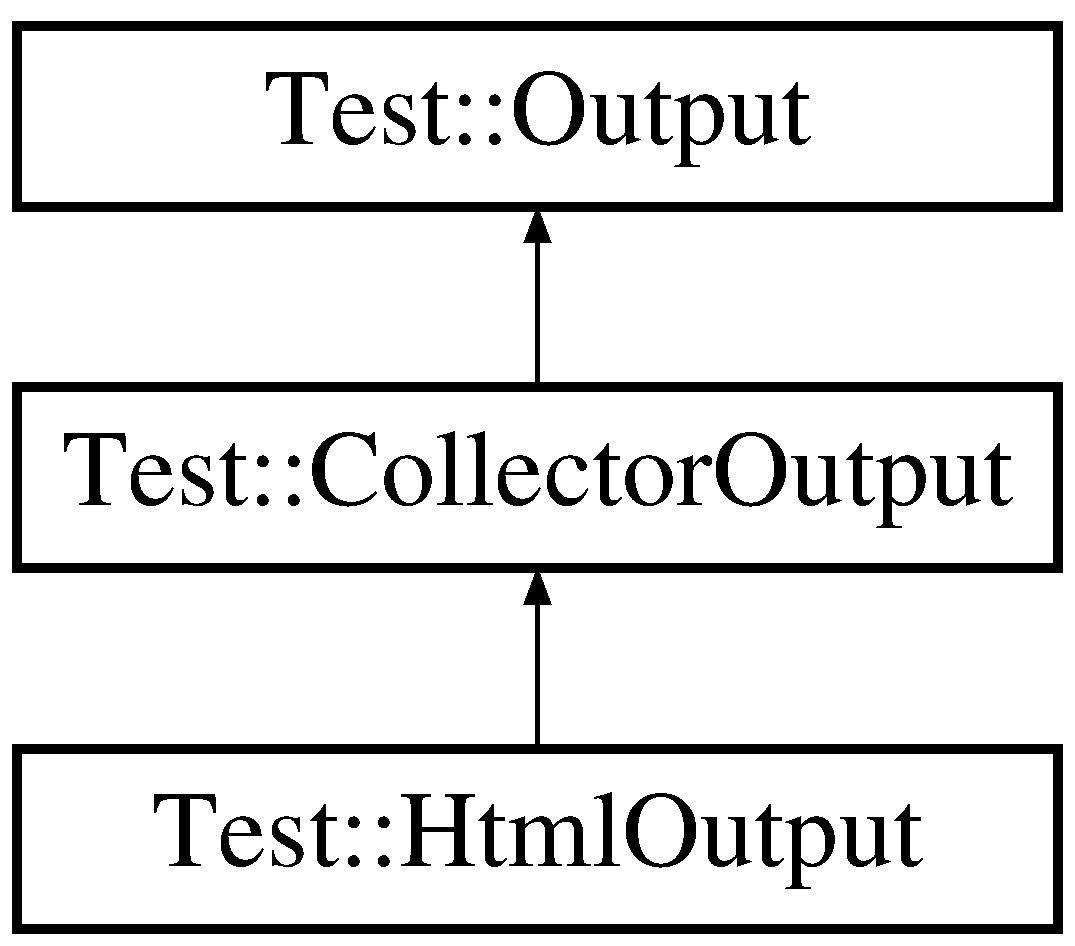
\includegraphics[height=3.000000cm]{class_test_1_1_html_output}
\end{center}
\end{figure}
\subsection*{Classes}
\begin{DoxyCompactItemize}
\item 
struct \hyperlink{struct_test_1_1_html_output_1_1_suite_row}{Suite\+Row}
\item 
struct \hyperlink{struct_test_1_1_html_output_1_1_suite_test_result}{Suite\+Test\+Result}
\item 
struct \hyperlink{struct_test_1_1_html_output_1_1_test_result}{Test\+Result}
\item 
struct \hyperlink{struct_test_1_1_html_output_1_1_test_result_all}{Test\+Result\+All}
\item 
struct \hyperlink{struct_test_1_1_html_output_1_1_test_row}{Test\+Row}
\item 
struct \hyperlink{struct_test_1_1_html_output_1_1_test_suite_row}{Test\+Suite\+Row}
\end{DoxyCompactItemize}
\subsection*{Public Member Functions}
\begin{DoxyCompactItemize}
\item 
void \hyperlink{class_test_1_1_html_output_a589e4e59aee4da0f70f3f6568daaf0f0}{generate} (std\+::ostream \&os, bool incl\+\_\+ok\+\_\+tests=true, const std\+::string \&name=\char`\"{}\char`\"{})
\end{DoxyCompactItemize}
\subsection*{Friends}
\begin{DoxyCompactItemize}
\item 
struct {\bfseries Test\+Suite\+Row}\hypertarget{class_test_1_1_html_output_a1e37e043f56a53b521955598f3366682}{}\label{class_test_1_1_html_output_a1e37e043f56a53b521955598f3366682}

\end{DoxyCompactItemize}
\subsection*{Additional Inherited Members}


\subsection{Detailed Description}
H\+T\+ML output. 

Output handler that creates a H\+T\+ML table with detailed information about all tests. 

Definition at line 44 of file cpptest-\/htmloutput.\+h.



\subsection{Member Function Documentation}
\index{Test\+::\+Html\+Output@{Test\+::\+Html\+Output}!generate@{generate}}
\index{generate@{generate}!Test\+::\+Html\+Output@{Test\+::\+Html\+Output}}
\subsubsection[{\texorpdfstring{generate(std\+::ostream \&os, bool incl\+\_\+ok\+\_\+tests=true, const std\+::string \&name="""")}{generate(std::ostream &os, bool incl_ok_tests=true, const std::string &name="")}}]{\setlength{\rightskip}{0pt plus 5cm}void Test\+::\+Html\+Output\+::generate (
\begin{DoxyParamCaption}
\item[{std\+::ostream \&}]{os, }
\item[{bool}]{incl\+\_\+ok\+\_\+tests = {\ttfamily true}, }
\item[{const std\+::string \&}]{name = {\ttfamily \char`\"{}\char`\"{}}}
\end{DoxyParamCaption}
)}\hypertarget{class_test_1_1_html_output_a589e4e59aee4da0f70f3f6568daaf0f0}{}\label{class_test_1_1_html_output_a589e4e59aee4da0f70f3f6568daaf0f0}
Generates the H\+T\+ML table. This function should only be called after run(), when all tests have been executed.


\begin{DoxyParams}{Parameters}
{\em os} & \hyperlink{class_test_1_1_output}{Output} stream. \\
\hline
{\em incl\+\_\+ok\+\_\+tests} & Set if successful tests should be shown; false otherwise. \\
\hline
{\em name} & Name of generated report. \\
\hline
\end{DoxyParams}


Definition at line 389 of file htmloutput.\+cpp.



The documentation for this class was generated from the following files\+:\begin{DoxyCompactItemize}
\item 
lib/cpptest-\/1.\+1.\+2/src/\hyperlink{cpptest-htmloutput_8h}{cpptest-\/htmloutput.\+h}\item 
lib/cpptest-\/1.\+1.\+2/src/htmloutput.\+cpp\end{DoxyCompactItemize}

\hypertarget{class_config_manager_1_1_integer_specifier}{}\section{Config\+Manager\+:\+:Integer\+Specifier Class Reference}
\label{class_config_manager_1_1_integer_specifier}\index{Config\+Manager\+::\+Integer\+Specifier@{Config\+Manager\+::\+Integer\+Specifier}}


{\ttfamily \#include $<$typespecifiers.\+h$>$}

Inheritance diagram for Config\+Manager\+:\+:Integer\+Specifier\+:\begin{figure}[H]
\begin{center}
\leavevmode
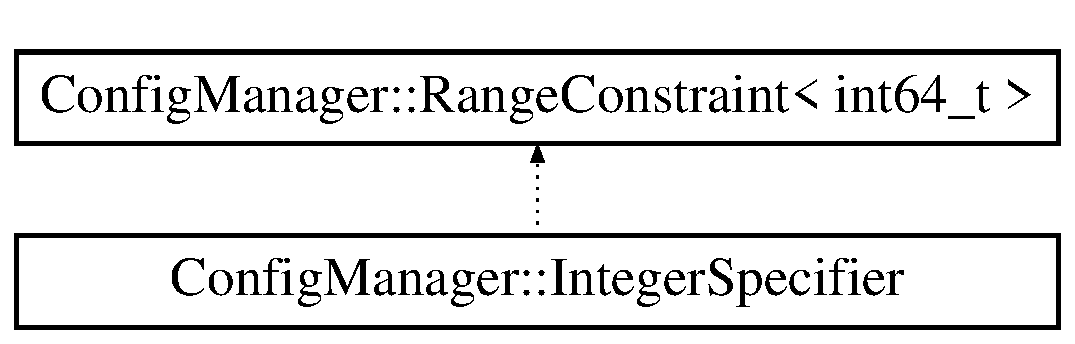
\includegraphics[height=2.000000cm]{class_config_manager_1_1_integer_specifier}
\end{center}
\end{figure}
\subsection*{Public Types}
\begin{DoxyCompactItemize}
\item 
typedef int64\+\_\+t \hyperlink{class_config_manager_1_1_integer_specifier_acebb8d401c86a80ca658d74dd25d8853}{Value\+Type}
\end{DoxyCompactItemize}
\subsection*{Public Member Functions}
\begin{DoxyCompactItemize}
\item 
\hyperlink{class_config_manager_1_1_integer_specifier_af2aa1191b70cb1ec8c85571e552c39e9}{Integer\+Specifier} ()
\item 
\hyperlink{class_config_manager_1_1_integer_specifier_a9c460b5b768882830ba440d3c8320f9e}{Integer\+Specifier} (int64\+\_\+t range\+\_\+start, int64\+\_\+t range\+\_\+end)
\item 
\hyperlink{class_config_manager_1_1_integer_specifier_acebb8d401c86a80ca658d74dd25d8853}{Value\+Type} \hyperlink{class_config_manager_1_1_integer_specifier_ade30bcb4b98b53b259e1a1e94cb5b882}{From\+String} (const std\+::string \&data)
\item 
std\+::string \hyperlink{class_config_manager_1_1_integer_specifier_ac61b72758b7221bffb9afd9e770013d3}{To\+String} (\hyperlink{class_config_manager_1_1_integer_specifier_acebb8d401c86a80ca658d74dd25d8853}{Value\+Type} value)
\end{DoxyCompactItemize}


\subsection{Detailed Description}
Trida realizujici prevod z textu do typu integer a zpet. 

Definition at line 91 of file typespecifiers.\+h.



\subsection{Member Typedef Documentation}
\index{Config\+Manager\+::\+Integer\+Specifier@{Config\+Manager\+::\+Integer\+Specifier}!Value\+Type@{Value\+Type}}
\index{Value\+Type@{Value\+Type}!Config\+Manager\+::\+Integer\+Specifier@{Config\+Manager\+::\+Integer\+Specifier}}
\subsubsection[{\texorpdfstring{Value\+Type}{ValueType}}]{\setlength{\rightskip}{0pt plus 5cm}typedef int64\+\_\+t {\bf Config\+Manager\+::\+Integer\+Specifier\+::\+Value\+Type}}\hypertarget{class_config_manager_1_1_integer_specifier_acebb8d401c86a80ca658d74dd25d8853}{}\label{class_config_manager_1_1_integer_specifier_acebb8d401c86a80ca658d74dd25d8853}




Tato definice typu urcuje navratovy typ. 

Definition at line 97 of file typespecifiers.\+h.



\subsection{Constructor \& Destructor Documentation}
\index{Config\+Manager\+::\+Integer\+Specifier@{Config\+Manager\+::\+Integer\+Specifier}!Integer\+Specifier@{Integer\+Specifier}}
\index{Integer\+Specifier@{Integer\+Specifier}!Config\+Manager\+::\+Integer\+Specifier@{Config\+Manager\+::\+Integer\+Specifier}}
\subsubsection[{\texorpdfstring{Integer\+Specifier()}{IntegerSpecifier()}}]{\setlength{\rightskip}{0pt plus 5cm}Config\+Manager\+::\+Integer\+Specifier\+::\+Integer\+Specifier (
\begin{DoxyParamCaption}
{}
\end{DoxyParamCaption}
)}\hypertarget{class_config_manager_1_1_integer_specifier_af2aa1191b70cb1ec8c85571e552c39e9}{}\label{class_config_manager_1_1_integer_specifier_af2aa1191b70cb1ec8c85571e552c39e9}
Konstruktor ktery neklade omezeni mezeni na rozsah hodnot. Rozsah hodnot je potom dan rozsahem zvoleneho typu. 

Definition at line 90 of file typespecifiers.\+cpp.

\index{Config\+Manager\+::\+Integer\+Specifier@{Config\+Manager\+::\+Integer\+Specifier}!Integer\+Specifier@{Integer\+Specifier}}
\index{Integer\+Specifier@{Integer\+Specifier}!Config\+Manager\+::\+Integer\+Specifier@{Config\+Manager\+::\+Integer\+Specifier}}
\subsubsection[{\texorpdfstring{Integer\+Specifier(int64\+\_\+t range\+\_\+start, int64\+\_\+t range\+\_\+end)}{IntegerSpecifier(int64_t range_start, int64_t range_end)}}]{\setlength{\rightskip}{0pt plus 5cm}Config\+Manager\+::\+Integer\+Specifier\+::\+Integer\+Specifier (
\begin{DoxyParamCaption}
\item[{int64\+\_\+t}]{range\+\_\+start, }
\item[{int64\+\_\+t}]{range\+\_\+end}
\end{DoxyParamCaption}
)}\hypertarget{class_config_manager_1_1_integer_specifier_a9c460b5b768882830ba440d3c8320f9e}{}\label{class_config_manager_1_1_integer_specifier_a9c460b5b768882830ba440d3c8320f9e}
Konstruktor ktery specifikuje rozsah pro vystupni parametry. ?? nema vyhazovat vyjimku kdyz range\+\_\+start $>$ range\+\_\+end? 
\begin{DoxyParams}{Parameters}
{\em range\+\_\+start} & dolni mez rozsahu. \\
\hline
{\em range\+\_\+end} & horni mez rozsahu. \\
\hline
\end{DoxyParams}


Definition at line 94 of file typespecifiers.\+cpp.



\subsection{Member Function Documentation}
\index{Config\+Manager\+::\+Integer\+Specifier@{Config\+Manager\+::\+Integer\+Specifier}!From\+String@{From\+String}}
\index{From\+String@{From\+String}!Config\+Manager\+::\+Integer\+Specifier@{Config\+Manager\+::\+Integer\+Specifier}}
\subsubsection[{\texorpdfstring{From\+String(const std\+::string \&data)}{FromString(const std::string &data)}}]{\setlength{\rightskip}{0pt plus 5cm}{\bf Integer\+Specifier\+::\+Value\+Type} Config\+Manager\+::\+Integer\+Specifier\+::\+From\+String (
\begin{DoxyParamCaption}
\item[{const std\+::string \&}]{data}
\end{DoxyParamCaption}
)}\hypertarget{class_config_manager_1_1_integer_specifier_ade30bcb4b98b53b259e1a1e94cb5b882}{}\label{class_config_manager_1_1_integer_specifier_ade30bcb4b98b53b259e1a1e94cb5b882}




Metoda prevadejici text na vyslednou hodnotu. Muze vyhodit \hyperlink{class_config_manager_1_1_wrong_format_exception}{Wrong\+Format\+Exception} vyjimku. 
\begin{DoxyParams}{Parameters}
{\em data} & Vstupni data. \\
\hline
\end{DoxyParams}


Definition at line 99 of file typespecifiers.\+cpp.

\index{Config\+Manager\+::\+Integer\+Specifier@{Config\+Manager\+::\+Integer\+Specifier}!To\+String@{To\+String}}
\index{To\+String@{To\+String}!Config\+Manager\+::\+Integer\+Specifier@{Config\+Manager\+::\+Integer\+Specifier}}
\subsubsection[{\texorpdfstring{To\+String(\+Value\+Type value)}{ToString(ValueType value)}}]{\setlength{\rightskip}{0pt plus 5cm}std\+::string Config\+Manager\+::\+Integer\+Specifier\+::\+To\+String (
\begin{DoxyParamCaption}
\item[{{\bf Integer\+Specifier\+::\+Value\+Type}}]{value}
\end{DoxyParamCaption}
)}\hypertarget{class_config_manager_1_1_integer_specifier_ac61b72758b7221bffb9afd9e770013d3}{}\label{class_config_manager_1_1_integer_specifier_ac61b72758b7221bffb9afd9e770013d3}






Definition at line 119 of file typespecifiers.\+cpp.



The documentation for this class was generated from the following files\+:\begin{DoxyCompactItemize}
\item 
E\+:/\+I\+N\+F\+O\+R\+M\+A\+T\+I\+K\+A/doporucene\+Postupy/uloha4/repos/src/\+Config\+Manager/typespecifiers.\+h\item 
E\+:/\+I\+N\+F\+O\+R\+M\+A\+T\+I\+K\+A/doporucene\+Postupy/uloha4/repos/src/\+Config\+Manager/typespecifiers.\+cpp\end{DoxyCompactItemize}

\hypertarget{class_test_1_1_compiler_output_1_1_invalid_format}{}\section{Test\+:\+:Compiler\+Output\+:\+:Invalid\+Format Class Reference}
\label{class_test_1_1_compiler_output_1_1_invalid_format}\index{Test\+::\+Compiler\+Output\+::\+Invalid\+Format@{Test\+::\+Compiler\+Output\+::\+Invalid\+Format}}


Compiler output exception.  




{\ttfamily \#include $<$cpptest-\/compileroutput.\+h$>$}

Inheritance diagram for Test\+:\+:Compiler\+Output\+:\+:Invalid\+Format\+:\begin{figure}[H]
\begin{center}
\leavevmode
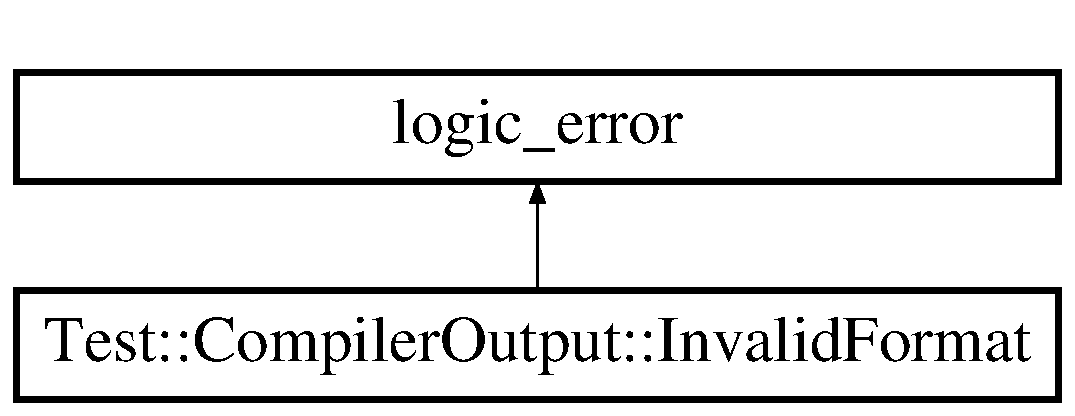
\includegraphics[height=2.000000cm]{class_test_1_1_compiler_output_1_1_invalid_format}
\end{center}
\end{figure}
\subsection*{Public Member Functions}
\begin{DoxyCompactItemize}
\item 
{\bfseries Invalid\+Format} (const std\+::string \&what)\hypertarget{class_test_1_1_compiler_output_1_1_invalid_format_a3a7ab44239805bcefd4bc19c48c91992}{}\label{class_test_1_1_compiler_output_1_1_invalid_format_a3a7ab44239805bcefd4bc19c48c91992}

\end{DoxyCompactItemize}


\subsection{Detailed Description}
Compiler output exception. 

Indicates that an invalid message format was given when creating a compiler output. The failing format may be retrieved using the what() method. 

Definition at line 61 of file cpptest-\/compileroutput.\+h.



The documentation for this class was generated from the following file\+:\begin{DoxyCompactItemize}
\item 
lib/cpptest-\/1.\+1.\+2/src/\hyperlink{cpptest-compileroutput_8h}{cpptest-\/compileroutput.\+h}\end{DoxyCompactItemize}

\hypertarget{class_config_manager_1_1_invalid_operation_exception}{}\section{Config\+Manager\+:\+:Invalid\+Operation\+Exception Class Reference}
\label{class_config_manager_1_1_invalid_operation_exception}\index{Config\+Manager\+::\+Invalid\+Operation\+Exception@{Config\+Manager\+::\+Invalid\+Operation\+Exception}}


{\ttfamily \#include $<$exceptions.\+h$>$}

Inheritance diagram for Config\+Manager\+:\+:Invalid\+Operation\+Exception\+:\begin{figure}[H]
\begin{center}
\leavevmode
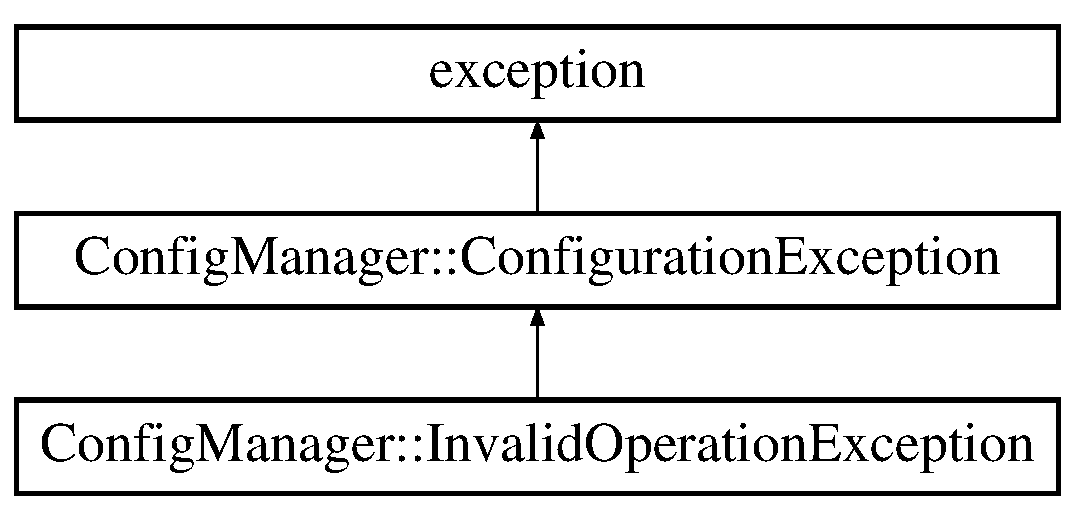
\includegraphics[height=3.000000cm]{class_config_manager_1_1_invalid_operation_exception}
\end{center}
\end{figure}
\subsection*{Public Member Functions}
\begin{DoxyCompactItemize}
\item 
{\bfseries Invalid\+Operation\+Exception} (const char $\ast$message)\hypertarget{class_config_manager_1_1_invalid_operation_exception_aee04fbcabd25794c25f1d245fd9d5f29}{}\label{class_config_manager_1_1_invalid_operation_exception_aee04fbcabd25794c25f1d245fd9d5f29}

\end{DoxyCompactItemize}


\subsection{Detailed Description}
Tato vyjimka je vyhoze v pripade, ze je specifikovana jiz pouzita sekce, ci pokud se uzivatel snazi vytvorit typ s minimalni hodnotou vetsi nez max, atd.. 

Definition at line 25 of file exceptions.\+h.



The documentation for this class was generated from the following file\+:\begin{DoxyCompactItemize}
\item 
E\+:/\+I\+N\+F\+O\+R\+M\+A\+T\+I\+K\+A/doporucene\+Postupy/uloha4/repos/src/\+Config\+Manager/exceptions.\+h\end{DoxyCompactItemize}

\hypertarget{class_config_manager_1_1_io_exception}{}\section{Config\+Manager\+:\+:Io\+Exception Class Reference}
\label{class_config_manager_1_1_io_exception}\index{Config\+Manager\+::\+Io\+Exception@{Config\+Manager\+::\+Io\+Exception}}
Inheritance diagram for Config\+Manager\+:\+:Io\+Exception\+:\begin{figure}[H]
\begin{center}
\leavevmode
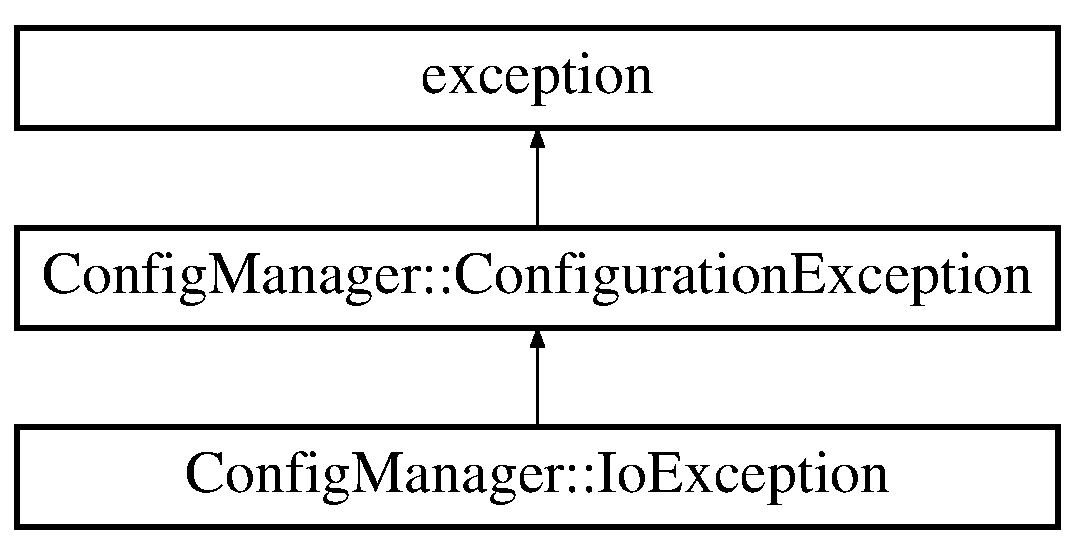
\includegraphics[height=3.000000cm]{class_config_manager_1_1_io_exception}
\end{center}
\end{figure}
\subsection*{Additional Inherited Members}


\subsection{Detailed Description}


Definition at line 33 of file exceptions.\+h.



The documentation for this class was generated from the following file\+:\begin{DoxyCompactItemize}
\item 
src/\+Config\+Manager/exceptions.\+h\end{DoxyCompactItemize}

\hypertarget{class_config_manager_1_1_list_option_proxy}{}\section{Config\+Manager\+:\+:List\+Option\+Proxy$<$ Type\+Specifier $>$ Class Template Reference}
\label{class_config_manager_1_1_list_option_proxy}\index{Config\+Manager\+::\+List\+Option\+Proxy$<$ Type\+Specifier $>$@{Config\+Manager\+::\+List\+Option\+Proxy$<$ Type\+Specifier $>$}}


{\ttfamily \#include $<$option.\+h$>$}

Inheritance diagram for Config\+Manager\+:\+:List\+Option\+Proxy$<$ Type\+Specifier $>$\+:\begin{figure}[H]
\begin{center}
\leavevmode
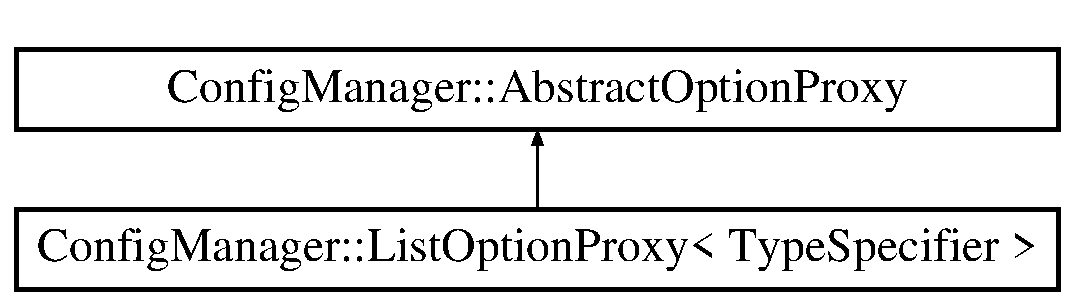
\includegraphics[height=2.000000cm]{class_config_manager_1_1_list_option_proxy}
\end{center}
\end{figure}
\subsection*{Public Member Functions}
\begin{DoxyCompactItemize}
\item 
\hyperlink{class_config_manager_1_1_list_option_proxy_ac277cb155b195258afe342f9efbffa7f}{List\+Option\+Proxy} (\hyperlink{class_config_manager_1_1_list_option_proxy}{List\+Option\+Proxy} \&\&other)
\item 
\hyperlink{class_config_manager_1_1_list_option_proxy}{List\+Option\+Proxy} \& \hyperlink{class_config_manager_1_1_list_option_proxy_a82c849b719e344486e0ef8c55afd28bc}{operator=} (\hyperlink{class_config_manager_1_1_list_option_proxy}{List\+Option\+Proxy} \&\&other)
\item 
std\+::size\+\_\+t \hyperlink{class_config_manager_1_1_list_option_proxy_a0abae5b24d1e43954b5d8c3d4ec942cc}{Count} ()
\item 
Item \hyperlink{class_config_manager_1_1_list_option_proxy_ab340c79edbe0da96cec77d46e571c3f0}{operator\mbox{[}$\,$\mbox{]}} (std\+::size\+\_\+t index)
\item 
Const\+Item \hyperlink{class_config_manager_1_1_list_option_proxy_a44365650affc4e1a117a01a8bce23ccb}{operator\mbox{[}$\,$\mbox{]}} (std\+::size\+\_\+t index) const 
\item 
Item \hyperlink{class_config_manager_1_1_list_option_proxy_a5a5207680997e76687527280474f6785}{Add} (const Value\+Type \&value)
\item 
Item \hyperlink{class_config_manager_1_1_list_option_proxy_af72aa3e07f55d22f46fbd542c68f20c9}{Insert} (std\+::size\+\_\+t index, const Value\+Type \&value)
\item 
void \hyperlink{class_config_manager_1_1_list_option_proxy_adf4052cfbba12a60b02601b63a618ae6}{Remove} (std\+::size\+\_\+t index)
\end{DoxyCompactItemize}
\subsection*{Protected Member Functions}
\begin{DoxyCompactItemize}
\item 
virtual void \hyperlink{class_config_manager_1_1_list_option_proxy_ab7d04f2f12da920861c6cef6d8dca501}{Regenerate\+Value\+Data} () override
\item 
virtual void \hyperlink{class_config_manager_1_1_list_option_proxy_ade1da6bf53c9bef0806755e4f805284e}{Process\+Value\+Data} (const std\+::string \&data) override
\end{DoxyCompactItemize}
\subsection*{Friends}
\begin{DoxyCompactItemize}
\item 
class {\bfseries Section}\hypertarget{class_config_manager_1_1_list_option_proxy_a0bd6fc422149e1c8416770631b28d40c}{}\label{class_config_manager_1_1_list_option_proxy_a0bd6fc422149e1c8416770631b28d40c}

\end{DoxyCompactItemize}


\subsection{Detailed Description}
\subsubsection*{template$<$typename Type\+Specifier$>$\\*
class Config\+Manager\+::\+List\+Option\+Proxy$<$ Type\+Specifier $>$}

Tato trida realizuje volbu tvorenou seznamem elementu. 

Definition at line 148 of file option.\+h.



\subsection{Constructor \& Destructor Documentation}
\index{Config\+Manager\+::\+List\+Option\+Proxy@{Config\+Manager\+::\+List\+Option\+Proxy}!List\+Option\+Proxy@{List\+Option\+Proxy}}
\index{List\+Option\+Proxy@{List\+Option\+Proxy}!Config\+Manager\+::\+List\+Option\+Proxy@{Config\+Manager\+::\+List\+Option\+Proxy}}
\subsubsection[{\texorpdfstring{List\+Option\+Proxy(\+List\+Option\+Proxy \&\&other)}{ListOptionProxy(ListOptionProxy &&other)}}]{\setlength{\rightskip}{0pt plus 5cm}template$<$typename Type\+Specifier $>$ {\bf Config\+Manager\+::\+List\+Option\+Proxy}$<$ {\bf Type\+Specifier} $>$\+::{\bf List\+Option\+Proxy} (
\begin{DoxyParamCaption}
\item[{{\bf List\+Option\+Proxy}$<$ {\bf Type\+Specifier} $>$ \&\&}]{other}
\end{DoxyParamCaption}
)}\hypertarget{class_config_manager_1_1_list_option_proxy_ac277cb155b195258afe342f9efbffa7f}{}\label{class_config_manager_1_1_list_option_proxy_ac277cb155b195258afe342f9efbffa7f}




Neni povoleno kopirovani instanci teto tridy. 

Definition at line 376 of file option.\+h.



\subsection{Member Function Documentation}
\index{Config\+Manager\+::\+List\+Option\+Proxy@{Config\+Manager\+::\+List\+Option\+Proxy}!Add@{Add}}
\index{Add@{Add}!Config\+Manager\+::\+List\+Option\+Proxy@{Config\+Manager\+::\+List\+Option\+Proxy}}
\subsubsection[{\texorpdfstring{Add(const Value\+Type \&value)}{Add(const ValueType &value)}}]{\setlength{\rightskip}{0pt plus 5cm}template$<$typename Type\+Specifier $>$ auto {\bf Config\+Manager\+::\+List\+Option\+Proxy}$<$ {\bf Type\+Specifier} $>$\+::Add (
\begin{DoxyParamCaption}
\item[{const Value\+Type \&}]{value}
\end{DoxyParamCaption}
)}\hypertarget{class_config_manager_1_1_list_option_proxy_a5a5207680997e76687527280474f6785}{}\label{class_config_manager_1_1_list_option_proxy_a5a5207680997e76687527280474f6785}
Metoda pro pridani nove volby do seznamu. 
\begin{DoxyParams}{Parameters}
{\em value} & Nova volba. \\
\hline
\end{DoxyParams}


Definition at line 450 of file option.\+h.

\index{Config\+Manager\+::\+List\+Option\+Proxy@{Config\+Manager\+::\+List\+Option\+Proxy}!Count@{Count}}
\index{Count@{Count}!Config\+Manager\+::\+List\+Option\+Proxy@{Config\+Manager\+::\+List\+Option\+Proxy}}
\subsubsection[{\texorpdfstring{Count()}{Count()}}]{\setlength{\rightskip}{0pt plus 5cm}template$<$typename Type\+Specifier $>$ std\+::size\+\_\+t {\bf Config\+Manager\+::\+List\+Option\+Proxy}$<$ {\bf Type\+Specifier} $>$\+::Count (
\begin{DoxyParamCaption}
{}
\end{DoxyParamCaption}
)}\hypertarget{class_config_manager_1_1_list_option_proxy_a0abae5b24d1e43954b5d8c3d4ec942cc}{}\label{class_config_manager_1_1_list_option_proxy_a0abae5b24d1e43954b5d8c3d4ec942cc}
Metoda vracejici pocet voleb v seznamu. 

Definition at line 427 of file option.\+h.

\index{Config\+Manager\+::\+List\+Option\+Proxy@{Config\+Manager\+::\+List\+Option\+Proxy}!Insert@{Insert}}
\index{Insert@{Insert}!Config\+Manager\+::\+List\+Option\+Proxy@{Config\+Manager\+::\+List\+Option\+Proxy}}
\subsubsection[{\texorpdfstring{Insert(std\+::size\+\_\+t index, const Value\+Type \&value)}{Insert(std::size_t index, const ValueType &value)}}]{\setlength{\rightskip}{0pt plus 5cm}template$<$typename Type\+Specifier $>$ auto {\bf Config\+Manager\+::\+List\+Option\+Proxy}$<$ {\bf Type\+Specifier} $>$\+::Insert (
\begin{DoxyParamCaption}
\item[{std\+::size\+\_\+t}]{index, }
\item[{const Value\+Type \&}]{value}
\end{DoxyParamCaption}
)}\hypertarget{class_config_manager_1_1_list_option_proxy_af72aa3e07f55d22f46fbd542c68f20c9}{}\label{class_config_manager_1_1_list_option_proxy_af72aa3e07f55d22f46fbd542c68f20c9}
Metoda pro pridani nove volby do seznamu. 
\begin{DoxyParams}{Parameters}
{\em value} & Nova volba. \\
\hline
\end{DoxyParams}


Definition at line 458 of file option.\+h.

\index{Config\+Manager\+::\+List\+Option\+Proxy@{Config\+Manager\+::\+List\+Option\+Proxy}!operator=@{operator=}}
\index{operator=@{operator=}!Config\+Manager\+::\+List\+Option\+Proxy@{Config\+Manager\+::\+List\+Option\+Proxy}}
\subsubsection[{\texorpdfstring{operator=(\+List\+Option\+Proxy \&\&other)}{operator=(ListOptionProxy &&other)}}]{\setlength{\rightskip}{0pt plus 5cm}template$<$typename Type\+Specifier $>$ {\bf List\+Option\+Proxy}$<$ {\bf Type\+Specifier} $>$ \& {\bf Config\+Manager\+::\+List\+Option\+Proxy}$<$ {\bf Type\+Specifier} $>$\+::operator= (
\begin{DoxyParamCaption}
\item[{{\bf List\+Option\+Proxy}$<$ {\bf Type\+Specifier} $>$ \&\&}]{other}
\end{DoxyParamCaption}
)}\hypertarget{class_config_manager_1_1_list_option_proxy_a82c849b719e344486e0ef8c55afd28bc}{}\label{class_config_manager_1_1_list_option_proxy_a82c849b719e344486e0ef8c55afd28bc}




Neni povoleno kopirovani instanci teto tridy. 

Definition at line 382 of file option.\+h.

\index{Config\+Manager\+::\+List\+Option\+Proxy@{Config\+Manager\+::\+List\+Option\+Proxy}!operator\mbox{[}$\,$\mbox{]}@{operator[]}}
\index{operator\mbox{[}$\,$\mbox{]}@{operator[]}!Config\+Manager\+::\+List\+Option\+Proxy@{Config\+Manager\+::\+List\+Option\+Proxy}}
\subsubsection[{\texorpdfstring{operator[](std\+::size\+\_\+t index)}{operator[](std::size_t index)}}]{\setlength{\rightskip}{0pt plus 5cm}template$<$typename Type\+Specifier $>$ auto {\bf Config\+Manager\+::\+List\+Option\+Proxy}$<$ {\bf Type\+Specifier} $>$\+::operator\mbox{[}$\,$\mbox{]} (
\begin{DoxyParamCaption}
\item[{std\+::size\+\_\+t}]{index}
\end{DoxyParamCaption}
)}\hypertarget{class_config_manager_1_1_list_option_proxy_ab340c79edbe0da96cec77d46e571c3f0}{}\label{class_config_manager_1_1_list_option_proxy_ab340c79edbe0da96cec77d46e571c3f0}
Operator pro pristup k jednotlivym volbam ze seznamu. Muze vyhodit \hyperlink{class_config_manager_1_1_out_of_bounds_exception}{Out\+Of\+Bounds\+Exception} vyjimku. 
\begin{DoxyParams}{Parameters}
{\em index} & Pozice pozadovane volby. \\
\hline
\end{DoxyParams}


Definition at line 433 of file option.\+h.

\index{Config\+Manager\+::\+List\+Option\+Proxy@{Config\+Manager\+::\+List\+Option\+Proxy}!operator\mbox{[}$\,$\mbox{]}@{operator[]}}
\index{operator\mbox{[}$\,$\mbox{]}@{operator[]}!Config\+Manager\+::\+List\+Option\+Proxy@{Config\+Manager\+::\+List\+Option\+Proxy}}
\subsubsection[{\texorpdfstring{operator[](std\+::size\+\_\+t index) const }{operator[](std::size_t index) const }}]{\setlength{\rightskip}{0pt plus 5cm}template$<$typename Type\+Specifier $>$ auto {\bf Config\+Manager\+::\+List\+Option\+Proxy}$<$ {\bf Type\+Specifier} $>$\+::operator\mbox{[}$\,$\mbox{]} (
\begin{DoxyParamCaption}
\item[{std\+::size\+\_\+t}]{index}
\end{DoxyParamCaption}
) const}\hypertarget{class_config_manager_1_1_list_option_proxy_a44365650affc4e1a117a01a8bce23ccb}{}\label{class_config_manager_1_1_list_option_proxy_a44365650affc4e1a117a01a8bce23ccb}
Operator pro konstantni pristup k jednotlivym volbam ze seznamu. Muze vyhodit \hyperlink{class_config_manager_1_1_out_of_bounds_exception}{Out\+Of\+Bounds\+Exception} vyjimku. 
\begin{DoxyParams}{Parameters}
{\em index} & Pozice pozadovane volby. \\
\hline
\end{DoxyParams}


Definition at line 441 of file option.\+h.

\index{Config\+Manager\+::\+List\+Option\+Proxy@{Config\+Manager\+::\+List\+Option\+Proxy}!Process\+Value\+Data@{Process\+Value\+Data}}
\index{Process\+Value\+Data@{Process\+Value\+Data}!Config\+Manager\+::\+List\+Option\+Proxy@{Config\+Manager\+::\+List\+Option\+Proxy}}
\subsubsection[{\texorpdfstring{Process\+Value\+Data(const std\+::string \&data) override}{ProcessValueData(const std::string &data) override}}]{\setlength{\rightskip}{0pt plus 5cm}template$<$typename Type\+Specifier $>$ void {\bf Config\+Manager\+::\+List\+Option\+Proxy}$<$ {\bf Type\+Specifier} $>$\+::Process\+Value\+Data (
\begin{DoxyParamCaption}
\item[{const std\+::string \&}]{data}
\end{DoxyParamCaption}
)\hspace{0.3cm}{\ttfamily [override]}, {\ttfamily [protected]}, {\ttfamily [virtual]}}\hypertarget{class_config_manager_1_1_list_option_proxy_ade1da6bf53c9bef0806755e4f805284e}{}\label{class_config_manager_1_1_list_option_proxy_ade1da6bf53c9bef0806755e4f805284e}




Metoda pro komunikaci s \hyperlink{class_config_manager_1_1_configuration}{Configuration} slouzici k aktualizaci hodnoty v Option\+Proxyu dle retezcove hodnoty v \hyperlink{class_config_manager_1_1_configuration}{Configuration}, iniciovane v \hyperlink{class_config_manager_1_1_configuration}{Configuration} (pripadne \hyperlink{class_config_manager_1_1_section}{Section}). 
\begin{DoxyParams}{Parameters}
{\em data} & Text ze ktereho ma byt hodnota prectena. \\
\hline
\end{DoxyParams}


Implements \hyperlink{class_config_manager_1_1_abstract_option_proxy_aeac427f8ddac8a9c17822022a3b1aaf1}{Config\+Manager\+::\+Abstract\+Option\+Proxy}.



Definition at line 498 of file option.\+h.

\index{Config\+Manager\+::\+List\+Option\+Proxy@{Config\+Manager\+::\+List\+Option\+Proxy}!Regenerate\+Value\+Data@{Regenerate\+Value\+Data}}
\index{Regenerate\+Value\+Data@{Regenerate\+Value\+Data}!Config\+Manager\+::\+List\+Option\+Proxy@{Config\+Manager\+::\+List\+Option\+Proxy}}
\subsubsection[{\texorpdfstring{Regenerate\+Value\+Data() override}{RegenerateValueData() override}}]{\setlength{\rightskip}{0pt plus 5cm}template$<$typename Type\+Specifier $>$ void {\bf Config\+Manager\+::\+List\+Option\+Proxy}$<$ {\bf Type\+Specifier} $>$\+::Regenerate\+Value\+Data (
\begin{DoxyParamCaption}
{}
\end{DoxyParamCaption}
)\hspace{0.3cm}{\ttfamily [override]}, {\ttfamily [protected]}, {\ttfamily [virtual]}}\hypertarget{class_config_manager_1_1_list_option_proxy_ab7d04f2f12da920861c6cef6d8dca501}{}\label{class_config_manager_1_1_list_option_proxy_ab7d04f2f12da920861c6cef6d8dca501}




Metoda pro komunikaci s \hyperlink{class_config_manager_1_1_configuration}{Configuration} slouzici pro vyvolani prepsani aktualni hodnoty v \hyperlink{class_config_manager_1_1_configuration}{Configuration} retezcovou reprezentaci hodnoty v Option\+Proxyu (lze tim zapsat default), iniciovane v \hyperlink{class_config_manager_1_1_configuration}{Configuration}. 

Implements \hyperlink{class_config_manager_1_1_abstract_option_proxy_aceb7b5e86f60c3dbd5b0622a230da1b3}{Config\+Manager\+::\+Abstract\+Option\+Proxy}.



Definition at line 478 of file option.\+h.

\index{Config\+Manager\+::\+List\+Option\+Proxy@{Config\+Manager\+::\+List\+Option\+Proxy}!Remove@{Remove}}
\index{Remove@{Remove}!Config\+Manager\+::\+List\+Option\+Proxy@{Config\+Manager\+::\+List\+Option\+Proxy}}
\subsubsection[{\texorpdfstring{Remove(std\+::size\+\_\+t index)}{Remove(std::size_t index)}}]{\setlength{\rightskip}{0pt plus 5cm}template$<$typename Type\+Specifier $>$ void {\bf Config\+Manager\+::\+List\+Option\+Proxy}$<$ {\bf Type\+Specifier} $>$\+::Remove (
\begin{DoxyParamCaption}
\item[{std\+::size\+\_\+t}]{index}
\end{DoxyParamCaption}
)}\hypertarget{class_config_manager_1_1_list_option_proxy_adf4052cfbba12a60b02601b63a618ae6}{}\label{class_config_manager_1_1_list_option_proxy_adf4052cfbba12a60b02601b63a618ae6}
Metoda pro odstraneni volby ze seznamu. 

Definition at line 468 of file option.\+h.



The documentation for this class was generated from the following file\+:\begin{DoxyCompactItemize}
\item 
E\+:/\+I\+N\+F\+O\+R\+M\+A\+T\+I\+K\+A/doporucene\+Postupy/uloha4/repos/src/\+Config\+Manager/option.\+h\end{DoxyCompactItemize}

\hypertarget{class_config_manager_1_1_malformed_input_exception}{}\section{Config\+Manager\+:\+:Malformed\+Input\+Exception Class Reference}
\label{class_config_manager_1_1_malformed_input_exception}\index{Config\+Manager\+::\+Malformed\+Input\+Exception@{Config\+Manager\+::\+Malformed\+Input\+Exception}}


{\ttfamily \#include $<$exceptions.\+h$>$}

Inheritance diagram for Config\+Manager\+:\+:Malformed\+Input\+Exception\+:\begin{figure}[H]
\begin{center}
\leavevmode
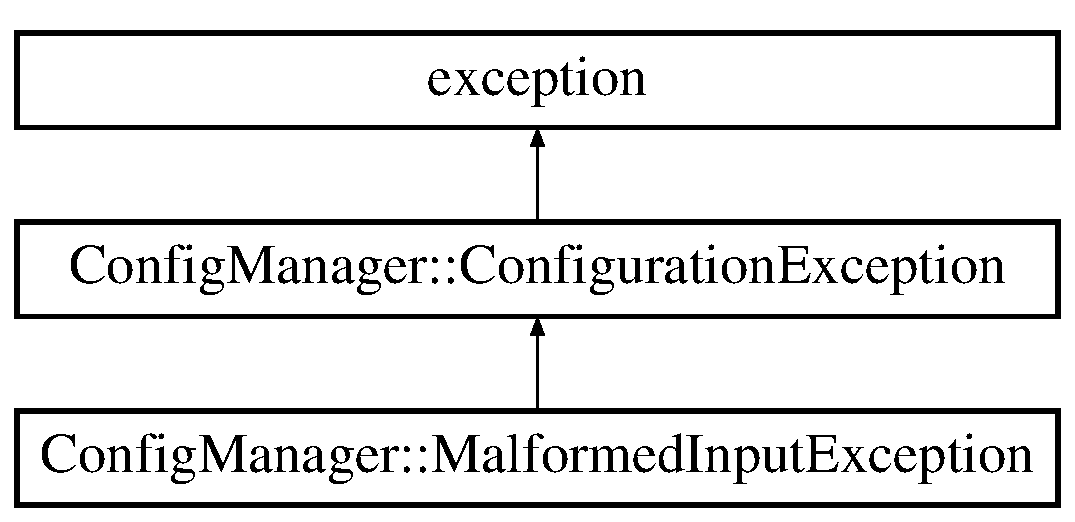
\includegraphics[height=3.000000cm]{class_config_manager_1_1_malformed_input_exception}
\end{center}
\end{figure}
\subsection*{Additional Inherited Members}


\subsection{Detailed Description}
Vyhazovana v pripade spatneho vstupu (spatne deklarace section ci option). 

Definition at line 34 of file exceptions.\+h.



The documentation for this class was generated from the following file\+:\begin{DoxyCompactItemize}
\item 
E\+:/\+I\+N\+F\+O\+R\+M\+A\+T\+I\+K\+A/doporucene\+Postupy/uloha4/repos/src/\+Config\+Manager/exceptions.\+h\end{DoxyCompactItemize}

\hypertarget{class_config_manager_1_1_mandatory_missing_exception}{}\section{Config\+Manager\+:\+:Mandatory\+Missing\+Exception Class Reference}
\label{class_config_manager_1_1_mandatory_missing_exception}\index{Config\+Manager\+::\+Mandatory\+Missing\+Exception@{Config\+Manager\+::\+Mandatory\+Missing\+Exception}}
Inheritance diagram for Config\+Manager\+:\+:Mandatory\+Missing\+Exception\+:\begin{figure}[H]
\begin{center}
\leavevmode
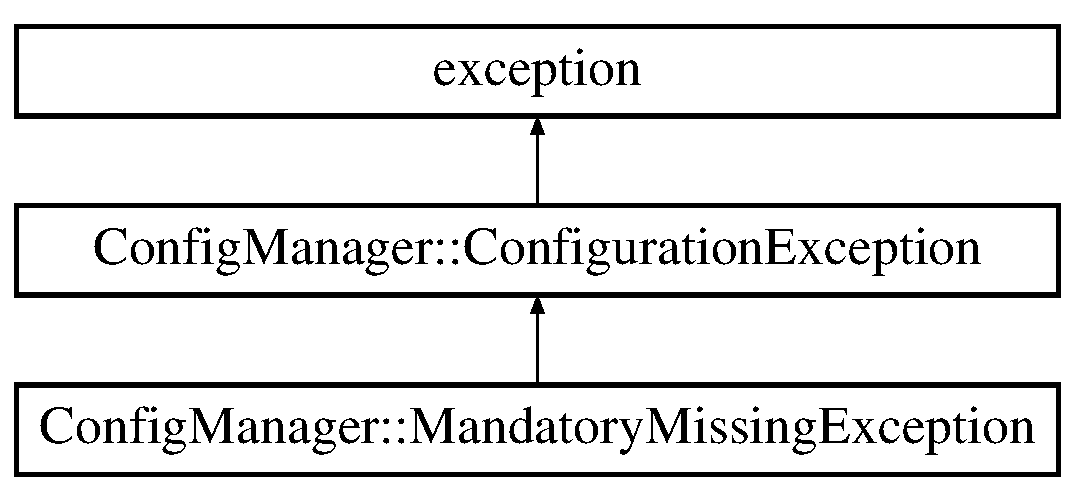
\includegraphics[height=3.000000cm]{class_config_manager_1_1_mandatory_missing_exception}
\end{center}
\end{figure}
\subsection*{Additional Inherited Members}


\subsection{Detailed Description}


Definition at line 53 of file exceptions.\+h.



The documentation for this class was generated from the following file\+:\begin{DoxyCompactItemize}
\item 
E\+:/\+I\+N\+F\+O\+R\+M\+A\+T\+I\+K\+A/doporucene\+Postupy/uloha4/repos/src/\+Config\+Manager/exceptions.\+h\end{DoxyCompactItemize}

\hypertarget{class_config_manager_1_1_option_node}{}\section{Config\+Manager\+:\+:Option\+Node Class Reference}
\label{class_config_manager_1_1_option_node}\index{Config\+Manager\+::\+Option\+Node@{Config\+Manager\+::\+Option\+Node}}


{\ttfamily \#include $<$optionnode.\+h$>$}

\subsection*{Public Member Functions}
\begin{DoxyCompactItemize}
\item 
\hyperlink{class_config_manager_1_1_option_node_a645c010a3f2e7e8f46cb5aab37d64e05}{Option\+Node} (const \hyperlink{class_config_manager_1_1_option_node}{Option\+Node} \&other)=delete
\item 
\hyperlink{class_config_manager_1_1_option_node}{Option\+Node} \& \hyperlink{class_config_manager_1_1_option_node_a8b5464fb5566388ebbb8ea614972d3ea}{operator=} (const \hyperlink{class_config_manager_1_1_option_node}{Option\+Node} \&other)=delete
\item 
void \hyperlink{class_config_manager_1_1_option_node_a552addaf613da2184eebee5580cdb72c}{Set\+Specified} ()
\item 
void \hyperlink{class_config_manager_1_1_option_node_a6b11e372911679bd045e3ee1f43cf4ba}{Set\+Proxy} (\hyperlink{class_config_manager_1_1_abstract_option_proxy}{Abstract\+Option\+Proxy} $\ast$proxy)
\item 
void \hyperlink{class_config_manager_1_1_option_node_adfb4172e5929b7927243b60ba8d28485}{Set\+Requirement} (Requirement requirement)
\item 
void \hyperlink{class_config_manager_1_1_option_node_a58f8440e7549ce5785db09886e79e2a5}{Set\+Comment} (const std\+::string \&comment)
\item 
const std\+::string \& \hyperlink{class_config_manager_1_1_option_node_af9e6b47860fc8718236e3fe29f043cd0}{Name} () const 
\item 
std\+::string \& \hyperlink{class_config_manager_1_1_option_node_aa33beb6d850388f3f6a41386d32164f1}{Value} ()
\item 
const std\+::string \& \hyperlink{class_config_manager_1_1_option_node_a3cbcb849cc14c06121f658b4aab2f8de}{Value} () const 
\item 
void \hyperlink{class_config_manager_1_1_option_node_a930987e088219ac5030621f2665493df}{Assign} (const std\+::string \&value)
\item 
\hyperlink{class_config_manager_1_1_section_node}{Section\+Node} \& \hyperlink{class_config_manager_1_1_option_node_a56ec62f82a04eeb275f711a38766a4b2}{Section} ()
\item 
const \hyperlink{class_config_manager_1_1_section_node}{Section\+Node} \& \hyperlink{class_config_manager_1_1_option_node_a5f04016950d1b512d1b3efad7558da13}{Section} () const 
\item 
bool \hyperlink{class_config_manager_1_1_option_node_a5c0a779da4931dab931cef2d9f9b1d70}{Is\+Loaded} () const 
\item 
bool \hyperlink{class_config_manager_1_1_option_node_aca68735af61349fb19341c3e06d02159}{Is\+Specified} () const 
\item 
bool \hyperlink{class_config_manager_1_1_option_node_a7a8275f01e9227e6192d485de7a28bdb}{Has\+Changed} () const 
\end{DoxyCompactItemize}


\subsection{Detailed Description}
Trida reprezentujici data volby v configuration. Muze a nemusi byt spojen s urcitou \hyperlink{class_config_manager_1_1_option_proxy}{Option\+Proxy} (\hyperlink{class_config_manager_1_1_list_option_proxy}{List\+Option\+Proxy}). Tato trida je urcena pouze pro vnitrni reprezentaci dat v knihovne. 

Definition at line 19 of file optionnode.\+h.



\subsection{Constructor \& Destructor Documentation}
\index{Config\+Manager\+::\+Option\+Node@{Config\+Manager\+::\+Option\+Node}!Option\+Node@{Option\+Node}}
\index{Option\+Node@{Option\+Node}!Config\+Manager\+::\+Option\+Node@{Config\+Manager\+::\+Option\+Node}}
\subsubsection[{\texorpdfstring{Option\+Node(const Option\+Node \&other)=delete}{OptionNode(const OptionNode &other)=delete}}]{\setlength{\rightskip}{0pt plus 5cm}Config\+Manager\+::\+Option\+Node\+::\+Option\+Node (
\begin{DoxyParamCaption}
\item[{const {\bf Option\+Node} \&}]{other}
\end{DoxyParamCaption}
)\hspace{0.3cm}{\ttfamily [delete]}}\hypertarget{class_config_manager_1_1_option_node_a645c010a3f2e7e8f46cb5aab37d64e05}{}\label{class_config_manager_1_1_option_node_a645c010a3f2e7e8f46cb5aab37d64e05}
Zakazany copy-\/constructor. 

\subsection{Member Function Documentation}
\index{Config\+Manager\+::\+Option\+Node@{Config\+Manager\+::\+Option\+Node}!Assign@{Assign}}
\index{Assign@{Assign}!Config\+Manager\+::\+Option\+Node@{Config\+Manager\+::\+Option\+Node}}
\subsubsection[{\texorpdfstring{Assign(const std\+::string \&value)}{Assign(const std::string &value)}}]{\setlength{\rightskip}{0pt plus 5cm}void Config\+Manager\+::\+Option\+Node\+::\+Assign (
\begin{DoxyParamCaption}
\item[{const std\+::string \&}]{value}
\end{DoxyParamCaption}
)}\hypertarget{class_config_manager_1_1_option_node_a930987e088219ac5030621f2665493df}{}\label{class_config_manager_1_1_option_node_a930987e088219ac5030621f2665493df}
Prirazeni hodnoty volby, oznacuje volbu jakozto zmenenou. 

Definition at line 54 of file optionnode.\+cpp.

\index{Config\+Manager\+::\+Option\+Node@{Config\+Manager\+::\+Option\+Node}!Has\+Changed@{Has\+Changed}}
\index{Has\+Changed@{Has\+Changed}!Config\+Manager\+::\+Option\+Node@{Config\+Manager\+::\+Option\+Node}}
\subsubsection[{\texorpdfstring{Has\+Changed() const }{HasChanged() const }}]{\setlength{\rightskip}{0pt plus 5cm}bool Config\+Manager\+::\+Option\+Node\+::\+Has\+Changed (
\begin{DoxyParamCaption}
{}
\end{DoxyParamCaption}
) const}\hypertarget{class_config_manager_1_1_option_node_a7a8275f01e9227e6192d485de7a28bdb}{}\label{class_config_manager_1_1_option_node_a7a8275f01e9227e6192d485de7a28bdb}
Dotaz, zda byla volba zmenena od sve puvodni (nactene, nebo vychozi) hodnoty. 

Definition at line 127 of file optionnode.\+cpp.

\index{Config\+Manager\+::\+Option\+Node@{Config\+Manager\+::\+Option\+Node}!Is\+Loaded@{Is\+Loaded}}
\index{Is\+Loaded@{Is\+Loaded}!Config\+Manager\+::\+Option\+Node@{Config\+Manager\+::\+Option\+Node}}
\subsubsection[{\texorpdfstring{Is\+Loaded() const }{IsLoaded() const }}]{\setlength{\rightskip}{0pt plus 5cm}bool Config\+Manager\+::\+Option\+Node\+::\+Is\+Loaded (
\begin{DoxyParamCaption}
{}
\end{DoxyParamCaption}
) const}\hypertarget{class_config_manager_1_1_option_node_a5c0a779da4931dab931cef2d9f9b1d70}{}\label{class_config_manager_1_1_option_node_a5c0a779da4931dab931cef2d9f9b1d70}
Dotaz, zda byl nacten z vstupnich dat (nebo je zatim jenom specifikovan). 

Definition at line 119 of file optionnode.\+cpp.

\index{Config\+Manager\+::\+Option\+Node@{Config\+Manager\+::\+Option\+Node}!Is\+Specified@{Is\+Specified}}
\index{Is\+Specified@{Is\+Specified}!Config\+Manager\+::\+Option\+Node@{Config\+Manager\+::\+Option\+Node}}
\subsubsection[{\texorpdfstring{Is\+Specified() const }{IsSpecified() const }}]{\setlength{\rightskip}{0pt plus 5cm}bool Config\+Manager\+::\+Option\+Node\+::\+Is\+Specified (
\begin{DoxyParamCaption}
{}
\end{DoxyParamCaption}
) const}\hypertarget{class_config_manager_1_1_option_node_aca68735af61349fb19341c3e06d02159}{}\label{class_config_manager_1_1_option_node_aca68735af61349fb19341c3e06d02159}
Dotaz, zda byla volba deklarovana uzivatelem. 

Definition at line 123 of file optionnode.\+cpp.

\index{Config\+Manager\+::\+Option\+Node@{Config\+Manager\+::\+Option\+Node}!Name@{Name}}
\index{Name@{Name}!Config\+Manager\+::\+Option\+Node@{Config\+Manager\+::\+Option\+Node}}
\subsubsection[{\texorpdfstring{Name() const }{Name() const }}]{\setlength{\rightskip}{0pt plus 5cm}const std\+::string \& Config\+Manager\+::\+Option\+Node\+::\+Name (
\begin{DoxyParamCaption}
{}
\end{DoxyParamCaption}
) const}\hypertarget{class_config_manager_1_1_option_node_af9e6b47860fc8718236e3fe29f043cd0}{}\label{class_config_manager_1_1_option_node_af9e6b47860fc8718236e3fe29f043cd0}
Jmeno volby. 

Definition at line 8 of file optionnode.\+cpp.

\index{Config\+Manager\+::\+Option\+Node@{Config\+Manager\+::\+Option\+Node}!operator=@{operator=}}
\index{operator=@{operator=}!Config\+Manager\+::\+Option\+Node@{Config\+Manager\+::\+Option\+Node}}
\subsubsection[{\texorpdfstring{operator=(const Option\+Node \&other)=delete}{operator=(const OptionNode &other)=delete}}]{\setlength{\rightskip}{0pt plus 5cm}{\bf Option\+Node}\& Config\+Manager\+::\+Option\+Node\+::operator= (
\begin{DoxyParamCaption}
\item[{const {\bf Option\+Node} \&}]{other}
\end{DoxyParamCaption}
)\hspace{0.3cm}{\ttfamily [delete]}}\hypertarget{class_config_manager_1_1_option_node_a8b5464fb5566388ebbb8ea614972d3ea}{}\label{class_config_manager_1_1_option_node_a8b5464fb5566388ebbb8ea614972d3ea}
Zakazany assign-\/constructor. \index{Config\+Manager\+::\+Option\+Node@{Config\+Manager\+::\+Option\+Node}!Section@{Section}}
\index{Section@{Section}!Config\+Manager\+::\+Option\+Node@{Config\+Manager\+::\+Option\+Node}}
\subsubsection[{\texorpdfstring{Section()}{Section()}}]{\setlength{\rightskip}{0pt plus 5cm}{\bf Section\+Node} \& Config\+Manager\+::\+Option\+Node\+::\+Section (
\begin{DoxyParamCaption}
{}
\end{DoxyParamCaption}
)}\hypertarget{class_config_manager_1_1_option_node_a56ec62f82a04eeb275f711a38766a4b2}{}\label{class_config_manager_1_1_option_node_a56ec62f82a04eeb275f711a38766a4b2}
Odkaz na sekci do ktere patri. 

Definition at line 60 of file optionnode.\+cpp.

\index{Config\+Manager\+::\+Option\+Node@{Config\+Manager\+::\+Option\+Node}!Section@{Section}}
\index{Section@{Section}!Config\+Manager\+::\+Option\+Node@{Config\+Manager\+::\+Option\+Node}}
\subsubsection[{\texorpdfstring{Section() const }{Section() const }}]{\setlength{\rightskip}{0pt plus 5cm}const {\bf Section\+Node} \& Config\+Manager\+::\+Option\+Node\+::\+Section (
\begin{DoxyParamCaption}
{}
\end{DoxyParamCaption}
) const}\hypertarget{class_config_manager_1_1_option_node_a5f04016950d1b512d1b3efad7558da13}{}\label{class_config_manager_1_1_option_node_a5f04016950d1b512d1b3efad7558da13}
Konstantni odkaz na sekci do ktere patri. 

Definition at line 65 of file optionnode.\+cpp.

\index{Config\+Manager\+::\+Option\+Node@{Config\+Manager\+::\+Option\+Node}!Set\+Comment@{Set\+Comment}}
\index{Set\+Comment@{Set\+Comment}!Config\+Manager\+::\+Option\+Node@{Config\+Manager\+::\+Option\+Node}}
\subsubsection[{\texorpdfstring{Set\+Comment(const std\+::string \&comment)}{SetComment(const std::string &comment)}}]{\setlength{\rightskip}{0pt plus 5cm}void Config\+Manager\+::\+Option\+Node\+::\+Set\+Comment (
\begin{DoxyParamCaption}
\item[{const std\+::string \&}]{comment}
\end{DoxyParamCaption}
)}\hypertarget{class_config_manager_1_1_option_node_a58f8440e7549ce5785db09886e79e2a5}{}\label{class_config_manager_1_1_option_node_a58f8440e7549ce5785db09886e79e2a5}
Nastavi kommentar. 
\begin{DoxyParams}{Parameters}
{\em Komentar.} & \\
\hline
\end{DoxyParams}


Definition at line 39 of file optionnode.\+cpp.

\index{Config\+Manager\+::\+Option\+Node@{Config\+Manager\+::\+Option\+Node}!Set\+Proxy@{Set\+Proxy}}
\index{Set\+Proxy@{Set\+Proxy}!Config\+Manager\+::\+Option\+Node@{Config\+Manager\+::\+Option\+Node}}
\subsubsection[{\texorpdfstring{Set\+Proxy(\+Abstract\+Option\+Proxy $\ast$proxy)}{SetProxy(AbstractOptionProxy *proxy)}}]{\setlength{\rightskip}{0pt plus 5cm}void Config\+Manager\+::\+Option\+Node\+::\+Set\+Proxy (
\begin{DoxyParamCaption}
\item[{{\bf Abstract\+Option\+Proxy} $\ast$}]{proxy}
\end{DoxyParamCaption}
)}\hypertarget{class_config_manager_1_1_option_node_a6b11e372911679bd045e3ee1f43cf4ba}{}\label{class_config_manager_1_1_option_node_a6b11e372911679bd045e3ee1f43cf4ba}
Nastavi spojeni s danou \hyperlink{class_config_manager_1_1_option_proxy}{Option\+Proxy}. 
\begin{DoxyParams}{Parameters}
{\em \hyperlink{class_config_manager_1_1_abstract_option_proxy}{Abstract\+Option\+Proxy}} & ktery odpovida temto datum. \\
\hline
\end{DoxyParams}


Definition at line 18 of file optionnode.\+cpp.

\index{Config\+Manager\+::\+Option\+Node@{Config\+Manager\+::\+Option\+Node}!Set\+Requirement@{Set\+Requirement}}
\index{Set\+Requirement@{Set\+Requirement}!Config\+Manager\+::\+Option\+Node@{Config\+Manager\+::\+Option\+Node}}
\subsubsection[{\texorpdfstring{Set\+Requirement(\+Requirement requirement)}{SetRequirement(Requirement requirement)}}]{\setlength{\rightskip}{0pt plus 5cm}void Config\+Manager\+::\+Option\+Node\+::\+Set\+Requirement (
\begin{DoxyParamCaption}
\item[{Requirement}]{requirement}
\end{DoxyParamCaption}
)}\hypertarget{class_config_manager_1_1_option_node_adfb4172e5929b7927243b60ba8d28485}{}\label{class_config_manager_1_1_option_node_adfb4172e5929b7927243b60ba8d28485}
Nastavi zda je dana volba v konfiguraci povinna. 
\begin{DoxyParams}{Parameters}
{\em Volab} & O\+P\+T\+I\+O\+N\+AL or M\+A\+N\+D\+A\+T\+O\+RY. \\
\hline
\end{DoxyParams}


Definition at line 23 of file optionnode.\+cpp.

\index{Config\+Manager\+::\+Option\+Node@{Config\+Manager\+::\+Option\+Node}!Set\+Specified@{Set\+Specified}}
\index{Set\+Specified@{Set\+Specified}!Config\+Manager\+::\+Option\+Node@{Config\+Manager\+::\+Option\+Node}}
\subsubsection[{\texorpdfstring{Set\+Specified()}{SetSpecified()}}]{\setlength{\rightskip}{0pt plus 5cm}void Config\+Manager\+::\+Option\+Node\+::\+Set\+Specified (
\begin{DoxyParamCaption}
{}
\end{DoxyParamCaption}
)}\hypertarget{class_config_manager_1_1_option_node_a552addaf613da2184eebee5580cdb72c}{}\label{class_config_manager_1_1_option_node_a552addaf613da2184eebee5580cdb72c}
Nastavi, ze existuje spojeni s \hyperlink{class_config_manager_1_1_option_proxy}{Option\+Proxy}. 

Definition at line 13 of file optionnode.\+cpp.

\index{Config\+Manager\+::\+Option\+Node@{Config\+Manager\+::\+Option\+Node}!Value@{Value}}
\index{Value@{Value}!Config\+Manager\+::\+Option\+Node@{Config\+Manager\+::\+Option\+Node}}
\subsubsection[{\texorpdfstring{Value()}{Value()}}]{\setlength{\rightskip}{0pt plus 5cm}std\+::string \& Config\+Manager\+::\+Option\+Node\+::\+Value (
\begin{DoxyParamCaption}
{}
\end{DoxyParamCaption}
)}\hypertarget{class_config_manager_1_1_option_node_aa33beb6d850388f3f6a41386d32164f1}{}\label{class_config_manager_1_1_option_node_aa33beb6d850388f3f6a41386d32164f1}
Stringova hodnota volby, primy pristup. 

Definition at line 44 of file optionnode.\+cpp.

\index{Config\+Manager\+::\+Option\+Node@{Config\+Manager\+::\+Option\+Node}!Value@{Value}}
\index{Value@{Value}!Config\+Manager\+::\+Option\+Node@{Config\+Manager\+::\+Option\+Node}}
\subsubsection[{\texorpdfstring{Value() const }{Value() const }}]{\setlength{\rightskip}{0pt plus 5cm}const std\+::string \& Config\+Manager\+::\+Option\+Node\+::\+Value (
\begin{DoxyParamCaption}
{}
\end{DoxyParamCaption}
) const}\hypertarget{class_config_manager_1_1_option_node_a3cbcb849cc14c06121f658b4aab2f8de}{}\label{class_config_manager_1_1_option_node_a3cbcb849cc14c06121f658b4aab2f8de}
Stringova hodnota volby, primiy (a konstantni) pristup. 

Definition at line 49 of file optionnode.\+cpp.



The documentation for this class was generated from the following files\+:\begin{DoxyCompactItemize}
\item 
E\+:/\+I\+N\+F\+O\+R\+M\+A\+T\+I\+K\+A/doporucene\+Postupy/uloha4/repos/src/\+Config\+Manager/optionnode.\+h\item 
E\+:/\+I\+N\+F\+O\+R\+M\+A\+T\+I\+K\+A/doporucene\+Postupy/uloha4/repos/src/\+Config\+Manager/optionnode.\+cpp\end{DoxyCompactItemize}

\hypertarget{class_config_manager_1_1_option_proxy}{}\section{Config\+Manager\+:\+:Option\+Proxy$<$ Type\+Specifier $>$ Class Template Reference}
\label{class_config_manager_1_1_option_proxy}\index{Config\+Manager\+::\+Option\+Proxy$<$ Type\+Specifier $>$@{Config\+Manager\+::\+Option\+Proxy$<$ Type\+Specifier $>$}}


{\ttfamily \#include $<$option.\+h$>$}

Inheritance diagram for Config\+Manager\+:\+:Option\+Proxy$<$ Type\+Specifier $>$\+:\begin{figure}[H]
\begin{center}
\leavevmode
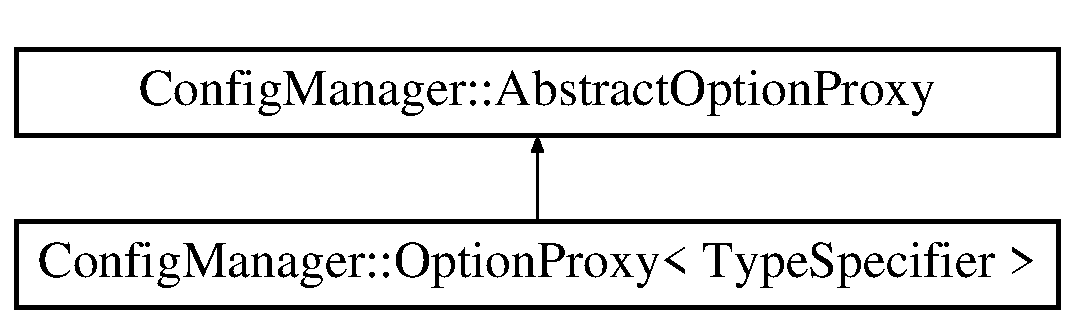
\includegraphics[height=2.000000cm]{class_config_manager_1_1_option_proxy}
\end{center}
\end{figure}
\subsection*{Public Member Functions}
\begin{DoxyCompactItemize}
\item 
\hyperlink{class_config_manager_1_1_option_proxy_ac72f87c50e3a887efb370d3d1249de8c}{Option\+Proxy} (\hyperlink{class_config_manager_1_1_option_proxy}{Option\+Proxy} \&\&other)
\item 
\hyperlink{class_config_manager_1_1_option_proxy}{Option\+Proxy} \& \hyperlink{class_config_manager_1_1_option_proxy_af571eb1d01be954f718adf22a6affcd1}{operator=} (\hyperlink{class_config_manager_1_1_option_proxy}{Option\+Proxy} \&\&other)
\item 
const Value\+Type \& \hyperlink{class_config_manager_1_1_option_proxy_a6c305bd6065c63e8b263660bf46ec727}{Get} () const 
\item 
void \hyperlink{class_config_manager_1_1_option_proxy_aa2be6bc353562df57f88ab222d38a2a3}{Set} (const Value\+Type \&value)
\end{DoxyCompactItemize}
\subsection*{Protected Member Functions}
\begin{DoxyCompactItemize}
\item 
virtual void \hyperlink{class_config_manager_1_1_option_proxy_a6f0f8c517701e7f55c2572e2deae6ad9}{Regenerate\+Value\+Data} () override
\item 
virtual void \hyperlink{class_config_manager_1_1_option_proxy_a41e884af79ba112250af76538cc38dc1}{Process\+Value\+Data} (const std\+::string \&data) override
\end{DoxyCompactItemize}
\subsection*{Friends}
\begin{DoxyCompactItemize}
\item 
class {\bfseries Section}\hypertarget{class_config_manager_1_1_option_proxy_a0bd6fc422149e1c8416770631b28d40c}{}\label{class_config_manager_1_1_option_proxy_a0bd6fc422149e1c8416770631b28d40c}

\end{DoxyCompactItemize}


\subsection{Detailed Description}
\subsubsection*{template$<$typename Type\+Specifier$>$\\*
class Config\+Manager\+::\+Option\+Proxy$<$ Type\+Specifier $>$}

Tato trida je realizuje volbu majici jednu hodnotu. 

Definition at line 95 of file option.\+h.



\subsection{Constructor \& Destructor Documentation}
\index{Config\+Manager\+::\+Option\+Proxy@{Config\+Manager\+::\+Option\+Proxy}!Option\+Proxy@{Option\+Proxy}}
\index{Option\+Proxy@{Option\+Proxy}!Config\+Manager\+::\+Option\+Proxy@{Config\+Manager\+::\+Option\+Proxy}}
\subsubsection[{\texorpdfstring{Option\+Proxy(\+Option\+Proxy \&\&other)}{OptionProxy(OptionProxy &&other)}}]{\setlength{\rightskip}{0pt plus 5cm}template$<$typename Type\+Specifier $>$ {\bf Config\+Manager\+::\+Option\+Proxy}$<$ {\bf Type\+Specifier} $>$\+::{\bf Option\+Proxy} (
\begin{DoxyParamCaption}
\item[{{\bf Option\+Proxy}$<$ {\bf Type\+Specifier} $>$ \&\&}]{other}
\end{DoxyParamCaption}
)}\hypertarget{class_config_manager_1_1_option_proxy_ac72f87c50e3a887efb370d3d1249de8c}{}\label{class_config_manager_1_1_option_proxy_ac72f87c50e3a887efb370d3d1249de8c}




Neni povoleno kopirovani instanci teto tridy. 

Definition at line 309 of file option.\+h.



\subsection{Member Function Documentation}
\index{Config\+Manager\+::\+Option\+Proxy@{Config\+Manager\+::\+Option\+Proxy}!Get@{Get}}
\index{Get@{Get}!Config\+Manager\+::\+Option\+Proxy@{Config\+Manager\+::\+Option\+Proxy}}
\subsubsection[{\texorpdfstring{Get() const }{Get() const }}]{\setlength{\rightskip}{0pt plus 5cm}template$<$typename Type\+Specifier $>$ auto {\bf Config\+Manager\+::\+Option\+Proxy}$<$ {\bf Type\+Specifier} $>$\+::Get (
\begin{DoxyParamCaption}
{}
\end{DoxyParamCaption}
) const}\hypertarget{class_config_manager_1_1_option_proxy_a6c305bd6065c63e8b263660bf46ec727}{}\label{class_config_manager_1_1_option_proxy_a6c305bd6065c63e8b263660bf46ec727}
Metoda vracejici nastavenou hodnotu. 

Definition at line 324 of file option.\+h.

\index{Config\+Manager\+::\+Option\+Proxy@{Config\+Manager\+::\+Option\+Proxy}!operator=@{operator=}}
\index{operator=@{operator=}!Config\+Manager\+::\+Option\+Proxy@{Config\+Manager\+::\+Option\+Proxy}}
\subsubsection[{\texorpdfstring{operator=(\+Option\+Proxy \&\&other)}{operator=(OptionProxy &&other)}}]{\setlength{\rightskip}{0pt plus 5cm}template$<$typename Type\+Specifier $>$ {\bf Option\+Proxy}$<$ {\bf Type\+Specifier} $>$ \& {\bf Config\+Manager\+::\+Option\+Proxy}$<$ {\bf Type\+Specifier} $>$\+::operator= (
\begin{DoxyParamCaption}
\item[{{\bf Option\+Proxy}$<$ {\bf Type\+Specifier} $>$ \&\&}]{other}
\end{DoxyParamCaption}
)}\hypertarget{class_config_manager_1_1_option_proxy_af571eb1d01be954f718adf22a6affcd1}{}\label{class_config_manager_1_1_option_proxy_af571eb1d01be954f718adf22a6affcd1}




Neni povoleno kopirovani instanci teto tridy. 

Definition at line 315 of file option.\+h.

\index{Config\+Manager\+::\+Option\+Proxy@{Config\+Manager\+::\+Option\+Proxy}!Process\+Value\+Data@{Process\+Value\+Data}}
\index{Process\+Value\+Data@{Process\+Value\+Data}!Config\+Manager\+::\+Option\+Proxy@{Config\+Manager\+::\+Option\+Proxy}}
\subsubsection[{\texorpdfstring{Process\+Value\+Data(const std\+::string \&data) override}{ProcessValueData(const std::string &data) override}}]{\setlength{\rightskip}{0pt plus 5cm}template$<$typename Type\+Specifier $>$ void {\bf Config\+Manager\+::\+Option\+Proxy}$<$ {\bf Type\+Specifier} $>$\+::Process\+Value\+Data (
\begin{DoxyParamCaption}
\item[{const std\+::string \&}]{data}
\end{DoxyParamCaption}
)\hspace{0.3cm}{\ttfamily [override]}, {\ttfamily [protected]}, {\ttfamily [virtual]}}\hypertarget{class_config_manager_1_1_option_proxy_a41e884af79ba112250af76538cc38dc1}{}\label{class_config_manager_1_1_option_proxy_a41e884af79ba112250af76538cc38dc1}




Metoda pro komunikaci s \hyperlink{class_config_manager_1_1_configuration}{Configuration} slouzici k aktualizaci hodnoty v Option\+Proxyu dle retezcove hodnoty v \hyperlink{class_config_manager_1_1_configuration}{Configuration}, iniciovane v \hyperlink{class_config_manager_1_1_configuration}{Configuration} (pripadne \hyperlink{class_config_manager_1_1_section}{Section}). 
\begin{DoxyParams}{Parameters}
{\em data} & Text ze ktereho ma byt hodnota prectena. \\
\hline
\end{DoxyParams}


Implements \hyperlink{class_config_manager_1_1_abstract_option_proxy_aeac427f8ddac8a9c17822022a3b1aaf1}{Config\+Manager\+::\+Abstract\+Option\+Proxy}.



Definition at line 343 of file option.\+h.

\index{Config\+Manager\+::\+Option\+Proxy@{Config\+Manager\+::\+Option\+Proxy}!Regenerate\+Value\+Data@{Regenerate\+Value\+Data}}
\index{Regenerate\+Value\+Data@{Regenerate\+Value\+Data}!Config\+Manager\+::\+Option\+Proxy@{Config\+Manager\+::\+Option\+Proxy}}
\subsubsection[{\texorpdfstring{Regenerate\+Value\+Data() override}{RegenerateValueData() override}}]{\setlength{\rightskip}{0pt plus 5cm}template$<$typename Type\+Specifier $>$ void {\bf Config\+Manager\+::\+Option\+Proxy}$<$ {\bf Type\+Specifier} $>$\+::Regenerate\+Value\+Data (
\begin{DoxyParamCaption}
{}
\end{DoxyParamCaption}
)\hspace{0.3cm}{\ttfamily [override]}, {\ttfamily [protected]}, {\ttfamily [virtual]}}\hypertarget{class_config_manager_1_1_option_proxy_a6f0f8c517701e7f55c2572e2deae6ad9}{}\label{class_config_manager_1_1_option_proxy_a6f0f8c517701e7f55c2572e2deae6ad9}




Metoda pro komunikaci s \hyperlink{class_config_manager_1_1_configuration}{Configuration} slouzici pro vyvolani prepsani aktualni hodnoty v \hyperlink{class_config_manager_1_1_configuration}{Configuration} retezcovou reprezentaci hodnoty v Option\+Proxyu (lze tim zapsat default), iniciovane v \hyperlink{class_config_manager_1_1_configuration}{Configuration}. 

Implements \hyperlink{class_config_manager_1_1_abstract_option_proxy_aceb7b5e86f60c3dbd5b0622a230da1b3}{Config\+Manager\+::\+Abstract\+Option\+Proxy}.



Definition at line 337 of file option.\+h.

\index{Config\+Manager\+::\+Option\+Proxy@{Config\+Manager\+::\+Option\+Proxy}!Set@{Set}}
\index{Set@{Set}!Config\+Manager\+::\+Option\+Proxy@{Config\+Manager\+::\+Option\+Proxy}}
\subsubsection[{\texorpdfstring{Set(const Value\+Type \&value)}{Set(const ValueType &value)}}]{\setlength{\rightskip}{0pt plus 5cm}template$<$typename Type\+Specifier $>$ void {\bf Config\+Manager\+::\+Option\+Proxy}$<$ {\bf Type\+Specifier} $>$\+::Set (
\begin{DoxyParamCaption}
\item[{const Value\+Type \&}]{value}
\end{DoxyParamCaption}
)}\hypertarget{class_config_manager_1_1_option_proxy_aa2be6bc353562df57f88ab222d38a2a3}{}\label{class_config_manager_1_1_option_proxy_aa2be6bc353562df57f88ab222d38a2a3}
Metoda pro nastaveni nove hodnoty volby. 
\begin{DoxyParams}{Parameters}
{\em value} & nova hodnota. \\
\hline
\end{DoxyParams}


Definition at line 330 of file option.\+h.



The documentation for this class was generated from the following file\+:\begin{DoxyCompactItemize}
\item 
E\+:/\+I\+N\+F\+O\+R\+M\+A\+T\+I\+K\+A/doporucene\+Postupy/uloha4/repos/src/\+Config\+Manager/option.\+h\end{DoxyCompactItemize}

\hypertarget{class_option_test_suite}{}\section{Option\+Test\+Suite Class Reference}
\label{class_option_test_suite}\index{Option\+Test\+Suite@{Option\+Test\+Suite}}
Inheritance diagram for Option\+Test\+Suite\+:\begin{figure}[H]
\begin{center}
\leavevmode
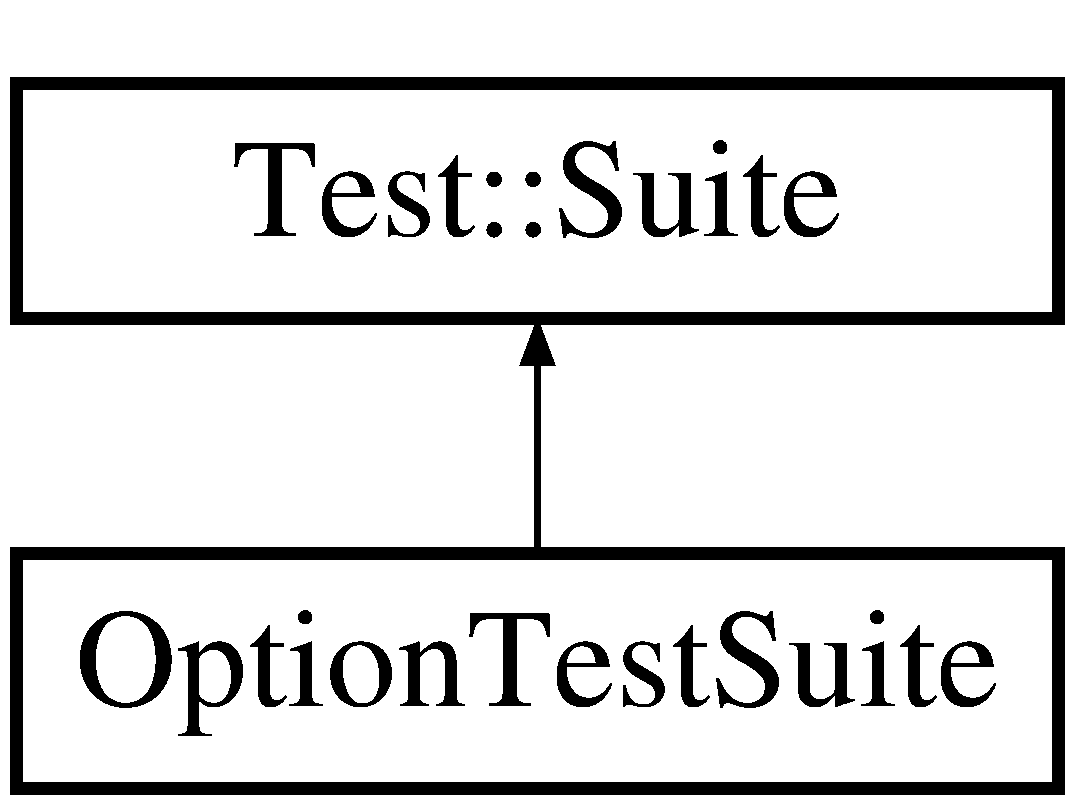
\includegraphics[height=2.000000cm]{class_option_test_suite}
\end{center}
\end{figure}
\subsection*{Additional Inherited Members}


\subsection{Detailed Description}


Definition at line 39 of file tests.\+h.



The documentation for this class was generated from the following files\+:\begin{DoxyCompactItemize}
\item 
tests/tests.\+h\item 
tests/tests.\+cpp\end{DoxyCompactItemize}

\hypertarget{class_config_manager_1_1_out_of_bounds_exception}{}\section{Config\+Manager\+:\+:Out\+Of\+Bounds\+Exception Class Reference}
\label{class_config_manager_1_1_out_of_bounds_exception}\index{Config\+Manager\+::\+Out\+Of\+Bounds\+Exception@{Config\+Manager\+::\+Out\+Of\+Bounds\+Exception}}


{\ttfamily \#include $<$exceptions.\+h$>$}

Inheritance diagram for Config\+Manager\+:\+:Out\+Of\+Bounds\+Exception\+:\begin{figure}[H]
\begin{center}
\leavevmode
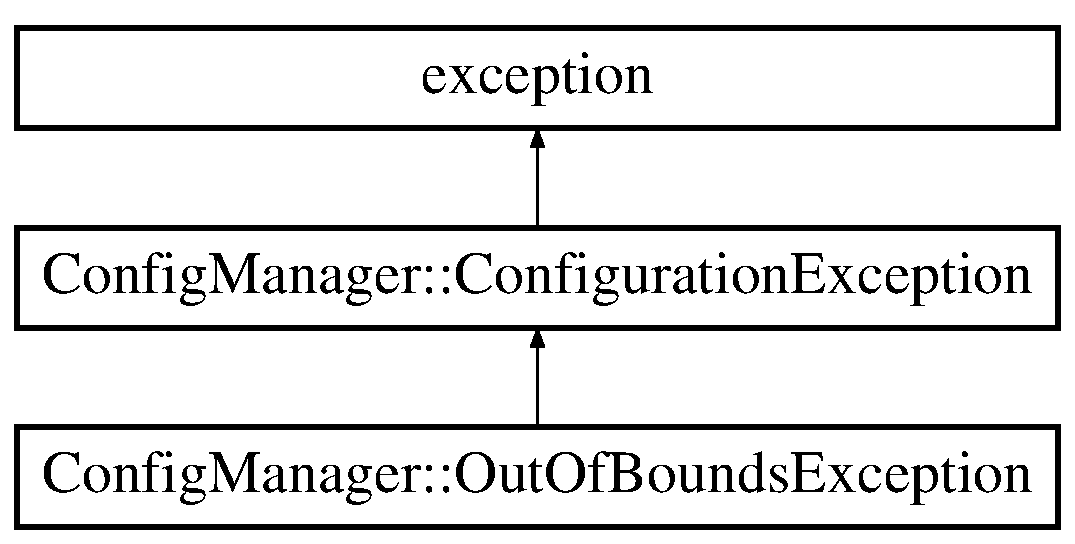
\includegraphics[height=3.000000cm]{class_config_manager_1_1_out_of_bounds_exception}
\end{center}
\end{figure}
\subsection*{Additional Inherited Members}


\subsection{Detailed Description}
Vyhazovan tridou \hyperlink{class_config_manager_1_1_list_option_proxy}{List\+Option\+Proxy}. 

Definition at line 90 of file exceptions.\+h.



The documentation for this class was generated from the following file\+:\begin{DoxyCompactItemize}
\item 
E\+:/\+I\+N\+F\+O\+R\+M\+A\+T\+I\+K\+A/doporucene\+Postupy/uloha4/repos/src/\+Config\+Manager/exceptions.\+h\end{DoxyCompactItemize}

\hypertarget{class_test_1_1_output}{}\section{Test\+:\+:Output Class Reference}
\label{class_test_1_1_output}\index{Test\+::\+Output@{Test\+::\+Output}}


Test suite output handler.  




{\ttfamily \#include $<$cpptest-\/output.\+h$>$}

Inheritance diagram for Test\+:\+:Output\+:\begin{figure}[H]
\begin{center}
\leavevmode
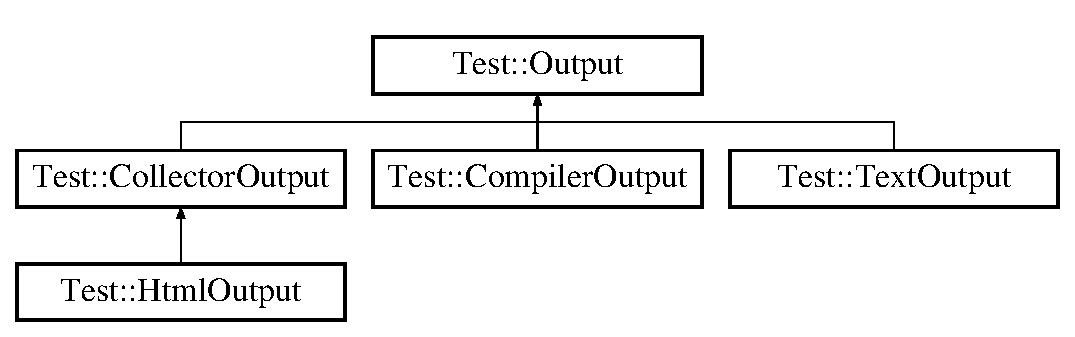
\includegraphics[height=3.000000cm]{class_test_1_1_output}
\end{center}
\end{figure}
\subsection*{Public Member Functions}
\begin{DoxyCompactItemize}
\item 
virtual \hyperlink{class_test_1_1_output_a838de994609ac3d13b7d7cd389f56090}{$\sim$\+Output} ()
\item 
virtual void \hyperlink{class_test_1_1_output_aa66480875d088befc6c23ecfd1107cc1}{initialize} (int tests)
\item 
virtual void \hyperlink{class_test_1_1_output_aeff8af8326a8c54a38199f76837f860a}{finished} (int tests, const \hyperlink{class_test_1_1_time}{Time} \&time)
\item 
virtual void \hyperlink{class_test_1_1_output_a7022c32c5a1577b10b93d3942746f17d}{suite\+\_\+start} (int tests, const std\+::string \&name)
\item 
virtual void \hyperlink{class_test_1_1_output_a6dbf4c0adb2bd4a7364c629179f788a6}{suite\+\_\+end} (int tests, const std\+::string \&name, const \hyperlink{class_test_1_1_time}{Time} \&time)
\item 
virtual void \hyperlink{class_test_1_1_output_a52d43b97609febc5abbc6da9aa0abac2}{test\+\_\+start} (const std\+::string \&name)
\item 
virtual void \hyperlink{class_test_1_1_output_a3796943e3b56373492c957212a21454e}{test\+\_\+end} (const std\+::string \&name, bool ok, const \hyperlink{class_test_1_1_time}{Time} \&time)
\item 
virtual void \hyperlink{class_test_1_1_output_a48c31f0baa7627d81939be840c9a7f65}{assertment} (const \hyperlink{class_test_1_1_source}{Source} \&s)
\end{DoxyCompactItemize}
\subsection*{Protected Member Functions}
\begin{DoxyCompactItemize}
\item 
\hyperlink{class_test_1_1_output_acbffb6b160039caafd3e9ac11cace65c}{Output} ()
\end{DoxyCompactItemize}


\subsection{Detailed Description}
Test suite output handler. 

Abstract base class for all suite output handlers. Derive from this class to create real output handlers that creates arbitrary complex output handlers.

All parts of testing is reported (test start/stop, suite start/stop, individual test start/stop, and assertments), thus giving maximum flexibility for derived classes. 

Definition at line 55 of file cpptest-\/output.\+h.



\subsection{Constructor \& Destructor Documentation}
\index{Test\+::\+Output@{Test\+::\+Output}!````~Output@{$\sim$\+Output}}
\index{````~Output@{$\sim$\+Output}!Test\+::\+Output@{Test\+::\+Output}}
\subsubsection[{\texorpdfstring{$\sim$\+Output()}{~Output()}}]{\setlength{\rightskip}{0pt plus 5cm}virtual Test\+::\+Output\+::$\sim$\+Output (
\begin{DoxyParamCaption}
{}
\end{DoxyParamCaption}
)\hspace{0.3cm}{\ttfamily [inline]}, {\ttfamily [virtual]}}\hypertarget{class_test_1_1_output_a838de994609ac3d13b7d7cd389f56090}{}\label{class_test_1_1_output_a838de994609ac3d13b7d7cd389f56090}
Empty destructor. 

Definition at line 60 of file cpptest-\/output.\+h.

\index{Test\+::\+Output@{Test\+::\+Output}!Output@{Output}}
\index{Output@{Output}!Test\+::\+Output@{Test\+::\+Output}}
\subsubsection[{\texorpdfstring{Output()}{Output()}}]{\setlength{\rightskip}{0pt plus 5cm}Test\+::\+Output\+::\+Output (
\begin{DoxyParamCaption}
{}
\end{DoxyParamCaption}
)\hspace{0.3cm}{\ttfamily [inline]}, {\ttfamily [protected]}}\hypertarget{class_test_1_1_output_acbffb6b160039caafd3e9ac11cace65c}{}\label{class_test_1_1_output_acbffb6b160039caafd3e9ac11cace65c}
Empty constructor. 

Definition at line 143 of file cpptest-\/output.\+h.



\subsection{Member Function Documentation}
\index{Test\+::\+Output@{Test\+::\+Output}!assertment@{assertment}}
\index{assertment@{assertment}!Test\+::\+Output@{Test\+::\+Output}}
\subsubsection[{\texorpdfstring{assertment(const Source \&s)}{assertment(const Source &s)}}]{\setlength{\rightskip}{0pt plus 5cm}virtual void Test\+::\+Output\+::assertment (
\begin{DoxyParamCaption}
\item[{const {\bf Source} \&}]{s}
\end{DoxyParamCaption}
)\hspace{0.3cm}{\ttfamily [inline]}, {\ttfamily [virtual]}}\hypertarget{class_test_1_1_output_a48c31f0baa7627d81939be840c9a7f65}{}\label{class_test_1_1_output_a48c31f0baa7627d81939be840c9a7f65}
Called when an assertment is issued.


\begin{DoxyParams}{Parameters}
{\em s} & Assert point information. \\
\hline
\end{DoxyParams}


Reimplemented in \hyperlink{class_test_1_1_compiler_output_ae276b6874eb54c8b1e3d8e3c610522dc}{Test\+::\+Compiler\+Output}, \hyperlink{class_test_1_1_text_output_a9acf66ddd0a5f584a86e5fbdd98e5f1a}{Test\+::\+Text\+Output}, and \hyperlink{class_test_1_1_collector_output_a201ecd71ad6e443b0be2e987d2dc3b39}{Test\+::\+Collector\+Output}.



Definition at line 135 of file cpptest-\/output.\+h.

\index{Test\+::\+Output@{Test\+::\+Output}!finished@{finished}}
\index{finished@{finished}!Test\+::\+Output@{Test\+::\+Output}}
\subsubsection[{\texorpdfstring{finished(int tests, const Time \&time)}{finished(int tests, const Time &time)}}]{\setlength{\rightskip}{0pt plus 5cm}virtual void Test\+::\+Output\+::finished (
\begin{DoxyParamCaption}
\item[{int}]{tests, }
\item[{const {\bf Time} \&}]{time}
\end{DoxyParamCaption}
)\hspace{0.3cm}{\ttfamily [inline]}, {\ttfamily [virtual]}}\hypertarget{class_test_1_1_output_aeff8af8326a8c54a38199f76837f860a}{}\label{class_test_1_1_output_aeff8af8326a8c54a38199f76837f860a}
Called when testing is finished.


\begin{DoxyParams}{Parameters}
{\em tests} & Total number of tests in all suites. \\
\hline
{\em time} & Total elapsed time for all tests. \\
\hline
\end{DoxyParams}


Reimplemented in \hyperlink{class_test_1_1_text_output_ad139154d84e75aaaabed7b718b0ff106}{Test\+::\+Text\+Output}, and \hyperlink{class_test_1_1_collector_output_a758efaaf1e348636cb3877c622d2b5d0}{Test\+::\+Collector\+Output}.



Definition at line 76 of file cpptest-\/output.\+h.

\index{Test\+::\+Output@{Test\+::\+Output}!initialize@{initialize}}
\index{initialize@{initialize}!Test\+::\+Output@{Test\+::\+Output}}
\subsubsection[{\texorpdfstring{initialize(int tests)}{initialize(int tests)}}]{\setlength{\rightskip}{0pt plus 5cm}virtual void Test\+::\+Output\+::initialize (
\begin{DoxyParamCaption}
\item[{int}]{tests}
\end{DoxyParamCaption}
)\hspace{0.3cm}{\ttfamily [inline]}, {\ttfamily [virtual]}}\hypertarget{class_test_1_1_output_aa66480875d088befc6c23ecfd1107cc1}{}\label{class_test_1_1_output_aa66480875d088befc6c23ecfd1107cc1}
Called when testing is started.


\begin{DoxyParams}{Parameters}
{\em tests} & Total number of tests in all suites. \\
\hline
\end{DoxyParams}


Definition at line 66 of file cpptest-\/output.\+h.

\index{Test\+::\+Output@{Test\+::\+Output}!suite\+\_\+end@{suite\+\_\+end}}
\index{suite\+\_\+end@{suite\+\_\+end}!Test\+::\+Output@{Test\+::\+Output}}
\subsubsection[{\texorpdfstring{suite\+\_\+end(int tests, const std\+::string \&name, const Time \&time)}{suite_end(int tests, const std::string &name, const Time &time)}}]{\setlength{\rightskip}{0pt plus 5cm}virtual void Test\+::\+Output\+::suite\+\_\+end (
\begin{DoxyParamCaption}
\item[{int}]{tests, }
\item[{const std\+::string \&}]{name, }
\item[{const {\bf Time} \&}]{time}
\end{DoxyParamCaption}
)\hspace{0.3cm}{\ttfamily [inline]}, {\ttfamily [virtual]}}\hypertarget{class_test_1_1_output_a6dbf4c0adb2bd4a7364c629179f788a6}{}\label{class_test_1_1_output_a6dbf4c0adb2bd4a7364c629179f788a6}
Called when a suite is finished.


\begin{DoxyParams}{Parameters}
{\em tests} & Number of tests in this suite. \\
\hline
{\em name} & Name of the suite. \\
\hline
{\em time} & Total elapsed time for all tests in this suite. \\
\hline
\end{DoxyParams}


Reimplemented in \hyperlink{class_test_1_1_text_output_a7687ec2e87ccaa901e2b7d391937a71e}{Test\+::\+Text\+Output}, and \hyperlink{class_test_1_1_collector_output_a25d129d55214c92189265a7bccd5b2cd}{Test\+::\+Collector\+Output}.



Definition at line 99 of file cpptest-\/output.\+h.

\index{Test\+::\+Output@{Test\+::\+Output}!suite\+\_\+start@{suite\+\_\+start}}
\index{suite\+\_\+start@{suite\+\_\+start}!Test\+::\+Output@{Test\+::\+Output}}
\subsubsection[{\texorpdfstring{suite\+\_\+start(int tests, const std\+::string \&name)}{suite_start(int tests, const std::string &name)}}]{\setlength{\rightskip}{0pt plus 5cm}virtual void Test\+::\+Output\+::suite\+\_\+start (
\begin{DoxyParamCaption}
\item[{int}]{tests, }
\item[{const std\+::string \&}]{name}
\end{DoxyParamCaption}
)\hspace{0.3cm}{\ttfamily [inline]}, {\ttfamily [virtual]}}\hypertarget{class_test_1_1_output_a7022c32c5a1577b10b93d3942746f17d}{}\label{class_test_1_1_output_a7022c32c5a1577b10b93d3942746f17d}
Called when a suite is entered.


\begin{DoxyParams}{Parameters}
{\em tests} & Number of tests in this suite. \\
\hline
{\em name} & Name of the suite. \\
\hline
\end{DoxyParams}


Reimplemented in \hyperlink{class_test_1_1_text_output_afa4d83846a506b7a26622711cbd69ad1}{Test\+::\+Text\+Output}, and \hyperlink{class_test_1_1_collector_output_ab4ea305009efd9e56c0549a04c9d55e6}{Test\+::\+Collector\+Output}.



Definition at line 87 of file cpptest-\/output.\+h.

\index{Test\+::\+Output@{Test\+::\+Output}!test\+\_\+end@{test\+\_\+end}}
\index{test\+\_\+end@{test\+\_\+end}!Test\+::\+Output@{Test\+::\+Output}}
\subsubsection[{\texorpdfstring{test\+\_\+end(const std\+::string \&name, bool ok, const Time \&time)}{test_end(const std::string &name, bool ok, const Time &time)}}]{\setlength{\rightskip}{0pt plus 5cm}virtual void Test\+::\+Output\+::test\+\_\+end (
\begin{DoxyParamCaption}
\item[{const std\+::string \&}]{name, }
\item[{bool}]{ok, }
\item[{const {\bf Time} \&}]{time}
\end{DoxyParamCaption}
)\hspace{0.3cm}{\ttfamily [inline]}, {\ttfamily [virtual]}}\hypertarget{class_test_1_1_output_a3796943e3b56373492c957212a21454e}{}\label{class_test_1_1_output_a3796943e3b56373492c957212a21454e}
Called when a test if finished, regardless if an assertment was issued.


\begin{DoxyParams}{Parameters}
{\em name} & Name of the test function. \\
\hline
{\em ok} & True if the test was successful; false otherwise. \\
\hline
{\em time} & Execution time. \\
\hline
\end{DoxyParams}


Reimplemented in \hyperlink{class_test_1_1_text_output_a61336a8ef939a9d826d4630da8020d72}{Test\+::\+Text\+Output}, and \hyperlink{class_test_1_1_collector_output_aa6f64879932cde17fc0098b8fc197c62}{Test\+::\+Collector\+Output}.



Definition at line 123 of file cpptest-\/output.\+h.

\index{Test\+::\+Output@{Test\+::\+Output}!test\+\_\+start@{test\+\_\+start}}
\index{test\+\_\+start@{test\+\_\+start}!Test\+::\+Output@{Test\+::\+Output}}
\subsubsection[{\texorpdfstring{test\+\_\+start(const std\+::string \&name)}{test_start(const std::string &name)}}]{\setlength{\rightskip}{0pt plus 5cm}virtual void Test\+::\+Output\+::test\+\_\+start (
\begin{DoxyParamCaption}
\item[{const std\+::string \&}]{name}
\end{DoxyParamCaption}
)\hspace{0.3cm}{\ttfamily [inline]}, {\ttfamily [virtual]}}\hypertarget{class_test_1_1_output_a52d43b97609febc5abbc6da9aa0abac2}{}\label{class_test_1_1_output_a52d43b97609febc5abbc6da9aa0abac2}
Called when a tests is executed.


\begin{DoxyParams}{Parameters}
{\em name} & Name of the test function. \\
\hline
\end{DoxyParams}


Reimplemented in \hyperlink{class_test_1_1_collector_output_a512aa60f06439a22c41dc5c3bfca15ff}{Test\+::\+Collector\+Output}.



Definition at line 111 of file cpptest-\/output.\+h.



The documentation for this class was generated from the following file\+:\begin{DoxyCompactItemize}
\item 
lib/cpptest-\/1.\+1.\+2/src/\hyperlink{cpptest-output_8h}{cpptest-\/output.\+h}\end{DoxyCompactItemize}

\hypertarget{class_config_manager_1_1_range_constraint}{}\section{Config\+Manager\+:\+:Range\+Constraint$<$ T\+Result $>$ Class Template Reference}
\label{class_config_manager_1_1_range_constraint}\index{Config\+Manager\+::\+Range\+Constraint$<$ T\+Result $>$@{Config\+Manager\+::\+Range\+Constraint$<$ T\+Result $>$}}
\subsection*{Public Member Functions}
\begin{DoxyCompactItemize}
\item 
{\bfseries Range\+Constraint} (const T\+Result \&range\+\_\+start, const T\+Result \&range\+\_\+end)\hypertarget{class_config_manager_1_1_range_constraint_a2a7a521c7b79ba43f6051592dc2bc61e}{}\label{class_config_manager_1_1_range_constraint_a2a7a521c7b79ba43f6051592dc2bc61e}

\item 
const T\+Result \& \hyperlink{class_config_manager_1_1_range_constraint_a71057f62a4735e80f1f1faacd7504069}{Check\+Constraint} (const T\+Result \&value)
\end{DoxyCompactItemize}


\subsection{Detailed Description}
\subsubsection*{template$<$typename T\+Result$>$\\*
class Config\+Manager\+::\+Range\+Constraint$<$ T\+Result $>$}



Definition at line 12 of file typespecifiers.\+h.



\subsection{Member Function Documentation}
\index{Config\+Manager\+::\+Range\+Constraint@{Config\+Manager\+::\+Range\+Constraint}!Check\+Constraint@{Check\+Constraint}}
\index{Check\+Constraint@{Check\+Constraint}!Config\+Manager\+::\+Range\+Constraint@{Config\+Manager\+::\+Range\+Constraint}}
\subsubsection[{\texorpdfstring{Check\+Constraint(const T\+Result \&value)}{CheckConstraint(const TResult &value)}}]{\setlength{\rightskip}{0pt plus 5cm}template$<$typename T\+Result$>$ const T\+Result \& {\bf Config\+Manager\+::\+Range\+Constraint}$<$ T\+Result $>$\+::Check\+Constraint (
\begin{DoxyParamCaption}
\item[{const T\+Result \&}]{value}
\end{DoxyParamCaption}
)}\hypertarget{class_config_manager_1_1_range_constraint_a71057f62a4735e80f1f1faacd7504069}{}\label{class_config_manager_1_1_range_constraint_a71057f62a4735e80f1f1faacd7504069}
Metoda provadejici kontrolu, zda je podminka popisovana tridou splnena. Pokud ano, vraci svuj parametr. Jinak vyhazuje vyjimku \hyperlink{class_config_manager_1_1_wrong_range_exception}{Wrong\+Range\+Exception}. 

Definition at line 259 of file typespecifiers.\+h.



The documentation for this class was generated from the following file\+:\begin{DoxyCompactItemize}
\item 
src/\+Config\+Manager/typespecifiers.\+h\end{DoxyCompactItemize}

\hypertarget{class_config_manager_1_1_section}{}\section{Config\+Manager\+:\+:Section Class Reference}
\label{class_config_manager_1_1_section}\index{Config\+Manager\+::\+Section@{Config\+Manager\+::\+Section}}


{\ttfamily \#include $<$section.\+h$>$}

\subsection*{Public Member Functions}
\begin{DoxyCompactItemize}
\item 
{\footnotesize template$<$typename Type\+Specifier $>$ }\\\hyperlink{class_config_manager_1_1_option_proxy}{Option\+Proxy}$<$ \hyperlink{class_config_manager_1_1_type_specifier}{Type\+Specifier} $>$ \hyperlink{class_config_manager_1_1_section_a94e7c5fe73d725c5cfdab6773f2ec00e}{Specify\+Option} (std\+::string option\+\_\+name, const \hyperlink{class_config_manager_1_1_type_specifier}{Type\+Specifier} \&type\+\_\+specifier, const typename \hyperlink{class_config_manager_1_1_type_specifier_a30331e624a3c4a1c18eb5b838e93acea}{Type\+Specifier\+::\+Value\+Type} \&default\+\_\+value, Requirement optional=Requirement\+::\+O\+P\+T\+I\+O\+N\+AL, const std\+::string \&comment=\char`\"{}\char`\"{})
\item 
{\footnotesize template$<$typename Type\+Specifier $>$ }\\\hyperlink{class_config_manager_1_1_list_option_proxy}{List\+Option\+Proxy}$<$ \hyperlink{class_config_manager_1_1_type_specifier}{Type\+Specifier} $>$ \hyperlink{class_config_manager_1_1_section_a3ebb197102f277aec4a012e073c8a0ca}{Specify\+List\+Option} (std\+::string option\+\_\+name, const \hyperlink{class_config_manager_1_1_type_specifier}{Type\+Specifier} \&type\+\_\+specifier, const std\+::vector$<$ typename \hyperlink{class_config_manager_1_1_type_specifier_a30331e624a3c4a1c18eb5b838e93acea}{Type\+Specifier\+::\+Value\+Type} $>$ \&default\+\_\+value, Requirement optional=Requirement\+::\+O\+P\+T\+I\+O\+N\+AL, const std\+::string \&comment=\char`\"{}\char`\"{})
\item 
const std\+::string \& \hyperlink{class_config_manager_1_1_section_a416bce47977331d53358a888f6995900}{Get\+Name} ()
\item 
std\+::string \hyperlink{class_config_manager_1_1_section_a99a220aa7baafa9131117c6b08b47506}{operator\mbox{[}$\,$\mbox{]}} (const std\+::string \&option\+\_\+name)
\end{DoxyCompactItemize}
\subsection*{Friends}
\begin{DoxyCompactItemize}
\item 
class {\bfseries Configuration}\hypertarget{class_config_manager_1_1_section_a30221ddc558692a7b52598b963a74bc2}{}\label{class_config_manager_1_1_section_a30221ddc558692a7b52598b963a74bc2}

\end{DoxyCompactItemize}


\subsection{Detailed Description}
Trida realizujici sekci voleb. Predavana ven z knihovny. 

Definition at line 16 of file section.\+h.



\subsection{Member Function Documentation}
\index{Config\+Manager\+::\+Section@{Config\+Manager\+::\+Section}!Get\+Name@{Get\+Name}}
\index{Get\+Name@{Get\+Name}!Config\+Manager\+::\+Section@{Config\+Manager\+::\+Section}}
\subsubsection[{\texorpdfstring{Get\+Name()}{GetName()}}]{\setlength{\rightskip}{0pt plus 5cm}const std\+::string \& Config\+Manager\+::\+Section\+::\+Get\+Name (
\begin{DoxyParamCaption}
{}
\end{DoxyParamCaption}
)}\hypertarget{class_config_manager_1_1_section_a416bce47977331d53358a888f6995900}{}\label{class_config_manager_1_1_section_a416bce47977331d53358a888f6995900}
Metoda pro pristup k jmenu sekce. 

Definition at line 11 of file section.\+cpp.

\index{Config\+Manager\+::\+Section@{Config\+Manager\+::\+Section}!operator\mbox{[}$\,$\mbox{]}@{operator[]}}
\index{operator\mbox{[}$\,$\mbox{]}@{operator[]}!Config\+Manager\+::\+Section@{Config\+Manager\+::\+Section}}
\subsubsection[{\texorpdfstring{operator[](const std\+::string \&option\+\_\+name)}{operator[](const std::string &option_name)}}]{\setlength{\rightskip}{0pt plus 5cm}std\+::string Config\+Manager\+::\+Section\+::operator\mbox{[}$\,$\mbox{]} (
\begin{DoxyParamCaption}
\item[{const std\+::string \&}]{option\+\_\+name}
\end{DoxyParamCaption}
)}\hypertarget{class_config_manager_1_1_section_a99a220aa7baafa9131117c6b08b47506}{}\label{class_config_manager_1_1_section_a99a220aa7baafa9131117c6b08b47506}
Primy pristup ke retezcove reprezentaci volby. 

Definition at line 16 of file section.\+cpp.

\index{Config\+Manager\+::\+Section@{Config\+Manager\+::\+Section}!Specify\+List\+Option@{Specify\+List\+Option}}
\index{Specify\+List\+Option@{Specify\+List\+Option}!Config\+Manager\+::\+Section@{Config\+Manager\+::\+Section}}
\subsubsection[{\texorpdfstring{Specify\+List\+Option(std\+::string option\+\_\+name, const Type\+Specifier \&type\+\_\+specifier, const std\+::vector$<$ typename Type\+Specifier\+::\+Value\+Type $>$ \&default\+\_\+value, Requirement optional=\+Requirement\+::\+O\+P\+T\+I\+O\+N\+A\+L, const std\+::string \&comment="""")}{SpecifyListOption(std::string option_name, const TypeSpecifier &type_specifier, const std::vector< typename TypeSpecifier::ValueType > &default_value, Requirement optional=Requirement::OPTIONAL, const std::string &comment="")}}]{\setlength{\rightskip}{0pt plus 5cm}template$<$typename Type\+Specifier $>$ {\bf List\+Option\+Proxy}$<$ {\bf Type\+Specifier} $>$ Config\+Manager\+::\+Section\+::\+Specify\+List\+Option (
\begin{DoxyParamCaption}
\item[{std\+::string}]{option\+\_\+name, }
\item[{const {\bf Type\+Specifier} \&}]{type\+\_\+specifier, }
\item[{const std\+::vector$<$ typename {\bf Type\+Specifier\+::\+Value\+Type} $>$ \&}]{default\+\_\+value, }
\item[{Requirement}]{optional = {\ttfamily Requirement\+:\+:OPTIONAL}, }
\item[{const std\+::string \&}]{comment = {\ttfamily \char`\"{}\char`\"{}}}
\end{DoxyParamCaption}
)}\hypertarget{class_config_manager_1_1_section_a3ebb197102f277aec4a012e073c8a0ca}{}\label{class_config_manager_1_1_section_a3ebb197102f277aec4a012e073c8a0ca}




Muze vyhodit \hyperlink{class_config_manager_1_1_wrong_format_exception}{Wrong\+Format\+Exception}, \hyperlink{class_config_manager_1_1_mandatory_missing_exception}{Mandatory\+Missing\+Exception} vyjimky. 

Definition at line 92 of file section.\+h.

\index{Config\+Manager\+::\+Section@{Config\+Manager\+::\+Section}!Specify\+Option@{Specify\+Option}}
\index{Specify\+Option@{Specify\+Option}!Config\+Manager\+::\+Section@{Config\+Manager\+::\+Section}}
\subsubsection[{\texorpdfstring{Specify\+Option(std\+::string option\+\_\+name, const Type\+Specifier \&type\+\_\+specifier, const typename Type\+Specifier\+::\+Value\+Type \&default\+\_\+value, Requirement optional=\+Requirement\+::\+O\+P\+T\+I\+O\+N\+A\+L, const std\+::string \&comment="""")}{SpecifyOption(std::string option_name, const TypeSpecifier &type_specifier, const typename TypeSpecifier::ValueType &default_value, Requirement optional=Requirement::OPTIONAL, const std::string &comment="")}}]{\setlength{\rightskip}{0pt plus 5cm}template$<$typename Type\+Specifier $>$ {\bf Option\+Proxy}$<$ {\bf Type\+Specifier} $>$ Config\+Manager\+::\+Section\+::\+Specify\+Option (
\begin{DoxyParamCaption}
\item[{std\+::string}]{option\+\_\+name, }
\item[{const {\bf Type\+Specifier} \&}]{type\+\_\+specifier, }
\item[{const typename {\bf Type\+Specifier\+::\+Value\+Type} \&}]{default\+\_\+value, }
\item[{Requirement}]{optional = {\ttfamily Requirement\+:\+:OPTIONAL}, }
\item[{const std\+::string \&}]{comment = {\ttfamily \char`\"{}\char`\"{}}}
\end{DoxyParamCaption}
)}\hypertarget{class_config_manager_1_1_section_a94e7c5fe73d725c5cfdab6773f2ec00e}{}\label{class_config_manager_1_1_section_a94e7c5fe73d725c5cfdab6773f2ec00e}
Metoda urcujici novou volbu v dane sekci. Muze vyhodit \hyperlink{class_config_manager_1_1_wrong_format_exception}{Wrong\+Format\+Exception}, \hyperlink{class_config_manager_1_1_mandatory_missing_exception}{Mandatory\+Missing\+Exception} vyjimky. 
\begin{DoxyParams}{Parameters}
{\em name} & Jmeno nove volby. \\
\hline
{\em type\+\_\+specifier} & Trida pro preklad volby z a do retezce. \\
\hline
{\em default\+\_\+value} & Prednastavena hodnota. \\
\hline
{\em optional} & Povinnost volby. \\
\hline
{\em comments} & Komentar. \\
\hline
\end{DoxyParams}


Definition at line 77 of file section.\+h.



The documentation for this class was generated from the following files\+:\begin{DoxyCompactItemize}
\item 
src/\+Config\+Manager/section.\+h\item 
src/\+Config\+Manager/section.\+cpp\end{DoxyCompactItemize}

\hypertarget{class_config_manager_1_1_section_node}{}\section{Config\+Manager\+:\+:Section\+Node Class Reference}
\label{class_config_manager_1_1_section_node}\index{Config\+Manager\+::\+Section\+Node@{Config\+Manager\+::\+Section\+Node}}
\subsection*{Public Member Functions}
\begin{DoxyCompactItemize}
\item 
{\bfseries Section\+Node} (const \hyperlink{class_config_manager_1_1_section_node}{Section\+Node} \&other)=delete\hypertarget{class_config_manager_1_1_section_node_a29c0bba247577ba6d163c07d54dcbe17}{}\label{class_config_manager_1_1_section_node_a29c0bba247577ba6d163c07d54dcbe17}

\item 
\hyperlink{class_config_manager_1_1_section_node}{Section\+Node} \& {\bfseries operator=} (const \hyperlink{class_config_manager_1_1_section_node}{Section\+Node} \&other)=delete\hypertarget{class_config_manager_1_1_section_node_ab4b00644db1b2b7fda5f7c3a331280be}{}\label{class_config_manager_1_1_section_node_ab4b00644db1b2b7fda5f7c3a331280be}

\item 
\hyperlink{class_config_manager_1_1_option_node}{Option\+Node} \& {\bfseries operator\mbox{[}$\,$\mbox{]}} (const std\+::string \&option\+\_\+name)\hypertarget{class_config_manager_1_1_section_node_a8516cbcb01048e0509f4cee76555aa43}{}\label{class_config_manager_1_1_section_node_a8516cbcb01048e0509f4cee76555aa43}

\item 
const \hyperlink{class_config_manager_1_1_option_node}{Option\+Node} \& {\bfseries operator\mbox{[}$\,$\mbox{]}} (const std\+::string \&option\+\_\+name) const \hypertarget{class_config_manager_1_1_section_node_a4ccb40813d717b21708254ace493cc26}{}\label{class_config_manager_1_1_section_node_a4ccb40813d717b21708254ace493cc26}

\item 
const std\+::string \& {\bfseries Name} () const \hypertarget{class_config_manager_1_1_section_node_ad8bec497af34b75f26128136a0342699}{}\label{class_config_manager_1_1_section_node_ad8bec497af34b75f26128136a0342699}

\item 
bool {\bfseries Is\+Loaded} () const \hypertarget{class_config_manager_1_1_section_node_ac557fc56f6d2cca4919949795c34abde}{}\label{class_config_manager_1_1_section_node_ac557fc56f6d2cca4919949795c34abde}

\end{DoxyCompactItemize}


\subsection{Detailed Description}


Definition at line 16 of file sectionnode.\+h.



The documentation for this class was generated from the following files\+:\begin{DoxyCompactItemize}
\item 
E\+:/\+I\+N\+F\+O\+R\+M\+A\+T\+I\+K\+A/doporucene\+Postupy/uloha4/repos/src/\+Config\+Manager/sectionnode.\+h\item 
E\+:/\+I\+N\+F\+O\+R\+M\+A\+T\+I\+K\+A/doporucene\+Postupy/uloha4/repos/src/\+Config\+Manager/sectionnode.\+cpp\end{DoxyCompactItemize}

\hypertarget{class_section_test_suite}{}\section{Section\+Test\+Suite Class Reference}
\label{class_section_test_suite}\index{Section\+Test\+Suite@{Section\+Test\+Suite}}
Inheritance diagram for Section\+Test\+Suite\+:\begin{figure}[H]
\begin{center}
\leavevmode
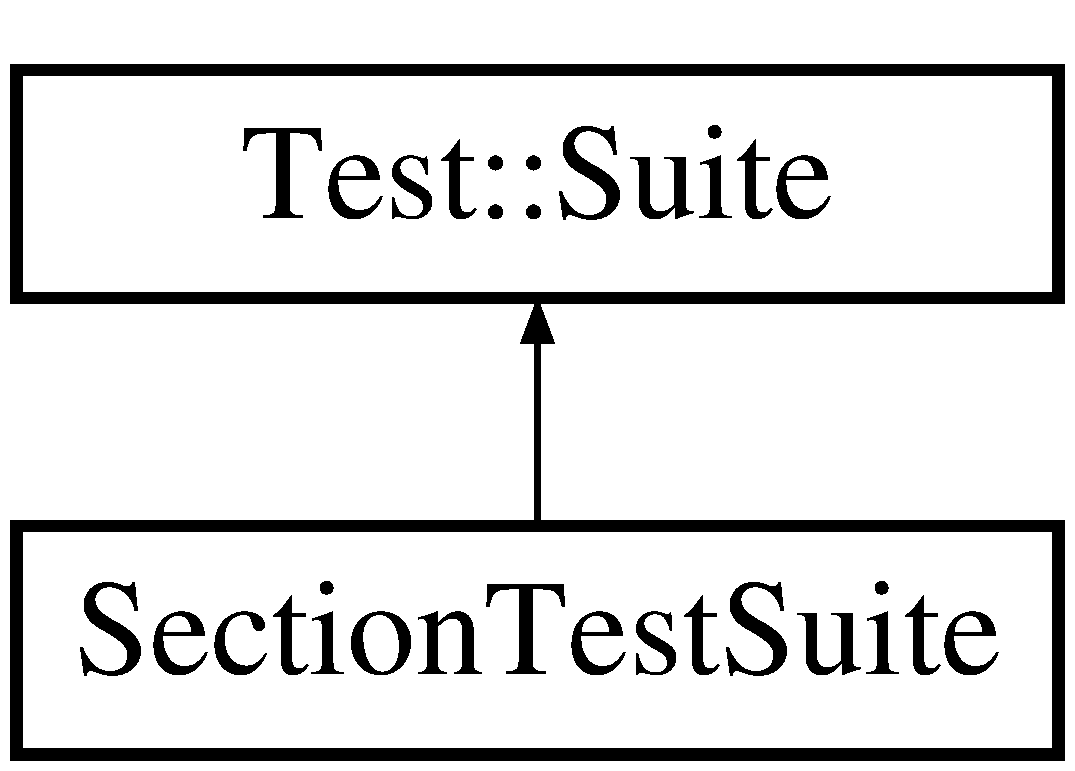
\includegraphics[height=2.000000cm]{class_section_test_suite}
\end{center}
\end{figure}
\subsection*{Additional Inherited Members}


\subsection{Detailed Description}


Definition at line 24 of file tests.\+h.



The documentation for this class was generated from the following files\+:\begin{DoxyCompactItemize}
\item 
tests/tests.\+h\item 
tests/tests.\+cpp\end{DoxyCompactItemize}

\hypertarget{class_test_1_1_source}{}\section{Test\+:\+:Source Class Reference}
\label{class_test_1_1_source}\index{Test\+::\+Source@{Test\+::\+Source}}


Assertment source information.  




{\ttfamily \#include $<$cpptest-\/source.\+h$>$}

\subsection*{Public Member Functions}
\begin{DoxyCompactItemize}
\item 
\hyperlink{class_test_1_1_source_abe0f303fe92270aa12a4a749ae0395ef}{Source} ()
\item 
\hyperlink{class_test_1_1_source_ac764beb685a574b81527d0f90ae9e428}{Source} (const char $\ast$\hyperlink{class_test_1_1_source_abb9d618ed57da70f177289b4bb035f02}{file}, unsigned int \hyperlink{class_test_1_1_source_aa61df0b07337fb411d67222669a8bc16}{line}, const char $\ast$msg)
\item 
const std\+::string \& \hyperlink{class_test_1_1_source_abb9d618ed57da70f177289b4bb035f02}{file} () const 
\item 
unsigned int \hyperlink{class_test_1_1_source_aa61df0b07337fb411d67222669a8bc16}{line} () const 
\item 
const std\+::string \& \hyperlink{class_test_1_1_source_adc700711d70f29ead5f5608dd6327ef2}{message} () const 
\item 
const std\+::string \& \hyperlink{class_test_1_1_source_a16e0a118d2d7af145a6169ff2b342290}{suite} () const 
\item 
const std\+::string \& \hyperlink{class_test_1_1_source_ab92c88c2842efb33daf97fe601a3653b}{test} () const 
\end{DoxyCompactItemize}
\subsection*{Friends}
\begin{DoxyCompactItemize}
\item 
class {\bfseries Suite}\hypertarget{class_test_1_1_source_a7de7b0dd89982bdae285f3a3b6197f9c}{}\label{class_test_1_1_source_a7de7b0dd89982bdae285f3a3b6197f9c}

\end{DoxyCompactItemize}


\subsection{Detailed Description}
Assertment source information. 

Contains information about an assertment point. 

Definition at line 42 of file cpptest-\/source.\+h.



\subsection{Constructor \& Destructor Documentation}
\index{Test\+::\+Source@{Test\+::\+Source}!Source@{Source}}
\index{Source@{Source}!Test\+::\+Source@{Test\+::\+Source}}
\subsubsection[{\texorpdfstring{Source()}{Source()}}]{\setlength{\rightskip}{0pt plus 5cm}Test\+::\+Source\+::\+Source (
\begin{DoxyParamCaption}
{}
\end{DoxyParamCaption}
)}\hypertarget{class_test_1_1_source_abe0f303fe92270aa12a4a749ae0395ef}{}\label{class_test_1_1_source_abe0f303fe92270aa12a4a749ae0395ef}
Constructs an invalid source object, which filename and message are empty strings and the line equals zero. 

Definition at line 36 of file source.\+cpp.

\index{Test\+::\+Source@{Test\+::\+Source}!Source@{Source}}
\index{Source@{Source}!Test\+::\+Source@{Test\+::\+Source}}
\subsubsection[{\texorpdfstring{Source(const char $\ast$file, unsigned int line, const char $\ast$msg)}{Source(const char *file, unsigned int line, const char *msg)}}]{\setlength{\rightskip}{0pt plus 5cm}Test\+::\+Source\+::\+Source (
\begin{DoxyParamCaption}
\item[{const char $\ast$}]{file, }
\item[{unsigned int}]{line, }
\item[{const char $\ast$}]{msg}
\end{DoxyParamCaption}
)}\hypertarget{class_test_1_1_source_ac764beb685a574b81527d0f90ae9e428}{}\label{class_test_1_1_source_ac764beb685a574b81527d0f90ae9e428}
Constructs a source object.


\begin{DoxyParams}{Parameters}
{\em file} & Name of the file containing the failing function. \\
\hline
{\em line} & Line where the function starts. \\
\hline
{\em msg} & Expression (or message) that caused the failure. \\
\hline
\end{DoxyParams}


Definition at line 46 of file source.\+cpp.



\subsection{Member Function Documentation}
\index{Test\+::\+Source@{Test\+::\+Source}!file@{file}}
\index{file@{file}!Test\+::\+Source@{Test\+::\+Source}}
\subsubsection[{\texorpdfstring{file() const }{file() const }}]{\setlength{\rightskip}{0pt plus 5cm}const string \& Test\+::\+Source\+::file (
\begin{DoxyParamCaption}
{}
\end{DoxyParamCaption}
) const}\hypertarget{class_test_1_1_source_abb9d618ed57da70f177289b4bb035f02}{}\label{class_test_1_1_source_abb9d618ed57da70f177289b4bb035f02}
\begin{DoxyReturn}{Returns}
Name of the file containing the failing function. 
\end{DoxyReturn}


Definition at line 55 of file source.\+cpp.

\index{Test\+::\+Source@{Test\+::\+Source}!line@{line}}
\index{line@{line}!Test\+::\+Source@{Test\+::\+Source}}
\subsubsection[{\texorpdfstring{line() const }{line() const }}]{\setlength{\rightskip}{0pt plus 5cm}unsigned int Test\+::\+Source\+::line (
\begin{DoxyParamCaption}
{}
\end{DoxyParamCaption}
) const}\hypertarget{class_test_1_1_source_aa61df0b07337fb411d67222669a8bc16}{}\label{class_test_1_1_source_aa61df0b07337fb411d67222669a8bc16}
\begin{DoxyReturn}{Returns}
Line where the function starts. 
\end{DoxyReturn}


Definition at line 63 of file source.\+cpp.

\index{Test\+::\+Source@{Test\+::\+Source}!message@{message}}
\index{message@{message}!Test\+::\+Source@{Test\+::\+Source}}
\subsubsection[{\texorpdfstring{message() const }{message() const }}]{\setlength{\rightskip}{0pt plus 5cm}const string \& Test\+::\+Source\+::message (
\begin{DoxyParamCaption}
{}
\end{DoxyParamCaption}
) const}\hypertarget{class_test_1_1_source_adc700711d70f29ead5f5608dd6327ef2}{}\label{class_test_1_1_source_adc700711d70f29ead5f5608dd6327ef2}
\begin{DoxyReturn}{Returns}
Descriptive message. 
\end{DoxyReturn}


Definition at line 71 of file source.\+cpp.

\index{Test\+::\+Source@{Test\+::\+Source}!suite@{suite}}
\index{suite@{suite}!Test\+::\+Source@{Test\+::\+Source}}
\subsubsection[{\texorpdfstring{suite() const }{suite() const }}]{\setlength{\rightskip}{0pt plus 5cm}const string \& Test\+::\+Source\+::suite (
\begin{DoxyParamCaption}
{}
\end{DoxyParamCaption}
) const}\hypertarget{class_test_1_1_source_a16e0a118d2d7af145a6169ff2b342290}{}\label{class_test_1_1_source_a16e0a118d2d7af145a6169ff2b342290}
\begin{DoxyReturn}{Returns}
Name of the suite, which the test belongs to. 
\end{DoxyReturn}


Definition at line 79 of file source.\+cpp.

\index{Test\+::\+Source@{Test\+::\+Source}!test@{test}}
\index{test@{test}!Test\+::\+Source@{Test\+::\+Source}}
\subsubsection[{\texorpdfstring{test() const }{test() const }}]{\setlength{\rightskip}{0pt plus 5cm}const string \& Test\+::\+Source\+::test (
\begin{DoxyParamCaption}
{}
\end{DoxyParamCaption}
) const}\hypertarget{class_test_1_1_source_ab92c88c2842efb33daf97fe601a3653b}{}\label{class_test_1_1_source_ab92c88c2842efb33daf97fe601a3653b}
\begin{DoxyReturn}{Returns}
Name of failing test. 
\end{DoxyReturn}


Definition at line 87 of file source.\+cpp.



The documentation for this class was generated from the following files\+:\begin{DoxyCompactItemize}
\item 
lib/cpptest-\/1.\+1.\+2/src/\hyperlink{cpptest-source_8h}{cpptest-\/source.\+h}\item 
lib/cpptest-\/1.\+1.\+2/src/source.\+cpp\end{DoxyCompactItemize}

\hypertarget{class_config_manager_1_1_strict_exception}{}\section{Config\+Manager\+:\+:Strict\+Exception Class Reference}
\label{class_config_manager_1_1_strict_exception}\index{Config\+Manager\+::\+Strict\+Exception@{Config\+Manager\+::\+Strict\+Exception}}
Inheritance diagram for Config\+Manager\+:\+:Strict\+Exception\+:\begin{figure}[H]
\begin{center}
\leavevmode
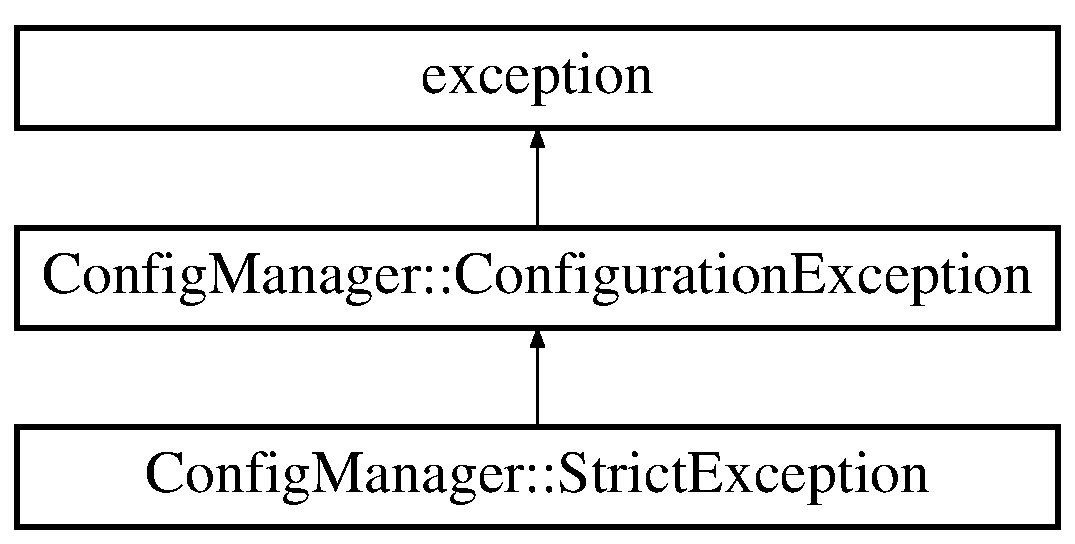
\includegraphics[height=3.000000cm]{class_config_manager_1_1_strict_exception}
\end{center}
\end{figure}
\subsection*{Additional Inherited Members}


\subsection{Detailed Description}


Definition at line 59 of file exceptions.\+h.



The documentation for this class was generated from the following file\+:\begin{DoxyCompactItemize}
\item 
E\+:/\+I\+N\+F\+O\+R\+M\+A\+T\+I\+K\+A/doporucene\+Postupy/uloha4/repos/src/\+Config\+Manager/exceptions.\+h\end{DoxyCompactItemize}

\hypertarget{class_config_manager_1_1_string_specifier}{}\section{Config\+Manager\+:\+:String\+Specifier Class Reference}
\label{class_config_manager_1_1_string_specifier}\index{Config\+Manager\+::\+String\+Specifier@{Config\+Manager\+::\+String\+Specifier}}


{\ttfamily \#include $<$typespecifiers.\+h$>$}

\subsection*{Public Types}
\begin{DoxyCompactItemize}
\item 
typedef std\+::string \hyperlink{class_config_manager_1_1_string_specifier_ac4bc384955f5da1874779f02c4ff757f}{Value\+Type}
\end{DoxyCompactItemize}
\subsection*{Public Member Functions}
\begin{DoxyCompactItemize}
\item 
\hyperlink{class_config_manager_1_1_string_specifier_a430e783d95729964c8a9a8755146805d}{String\+Specifier} ()
\item 
const \hyperlink{class_config_manager_1_1_string_specifier_ac4bc384955f5da1874779f02c4ff757f}{Value\+Type} \& \hyperlink{class_config_manager_1_1_string_specifier_aced30df1ae4ec0922f3fd87a98b4ca65}{From\+String} (const std\+::string \&data)
\item 
const std\+::string \& \hyperlink{class_config_manager_1_1_string_specifier_a86ad1a911411e7189c55056f7369355d}{To\+String} (const \hyperlink{class_config_manager_1_1_string_specifier_ac4bc384955f5da1874779f02c4ff757f}{Value\+Type} \&value)
\end{DoxyCompactItemize}


\subsection{Detailed Description}
Trida realizujici prevod z textu do typu string a zpet. 

Definition at line 217 of file typespecifiers.\+h.



\subsection{Member Typedef Documentation}
\index{Config\+Manager\+::\+String\+Specifier@{Config\+Manager\+::\+String\+Specifier}!Value\+Type@{Value\+Type}}
\index{Value\+Type@{Value\+Type}!Config\+Manager\+::\+String\+Specifier@{Config\+Manager\+::\+String\+Specifier}}
\subsubsection[{\texorpdfstring{Value\+Type}{ValueType}}]{\setlength{\rightskip}{0pt plus 5cm}typedef std\+::string {\bf Config\+Manager\+::\+String\+Specifier\+::\+Value\+Type}}\hypertarget{class_config_manager_1_1_string_specifier_ac4bc384955f5da1874779f02c4ff757f}{}\label{class_config_manager_1_1_string_specifier_ac4bc384955f5da1874779f02c4ff757f}




Tato definice typu urcuje navratovy typ. 

Definition at line 223 of file typespecifiers.\+h.



\subsection{Constructor \& Destructor Documentation}
\index{Config\+Manager\+::\+String\+Specifier@{Config\+Manager\+::\+String\+Specifier}!String\+Specifier@{String\+Specifier}}
\index{String\+Specifier@{String\+Specifier}!Config\+Manager\+::\+String\+Specifier@{Config\+Manager\+::\+String\+Specifier}}
\subsubsection[{\texorpdfstring{String\+Specifier()}{StringSpecifier()}}]{\setlength{\rightskip}{0pt plus 5cm}Config\+Manager\+::\+String\+Specifier\+::\+String\+Specifier (
\begin{DoxyParamCaption}
{}
\end{DoxyParamCaption}
)}\hypertarget{class_config_manager_1_1_string_specifier_a430e783d95729964c8a9a8755146805d}{}\label{class_config_manager_1_1_string_specifier_a430e783d95729964c8a9a8755146805d}
Zakladni konstruktor. 

Definition at line 198 of file typespecifiers.\+cpp.



\subsection{Member Function Documentation}
\index{Config\+Manager\+::\+String\+Specifier@{Config\+Manager\+::\+String\+Specifier}!From\+String@{From\+String}}
\index{From\+String@{From\+String}!Config\+Manager\+::\+String\+Specifier@{Config\+Manager\+::\+String\+Specifier}}
\subsubsection[{\texorpdfstring{From\+String(const std\+::string \&data)}{FromString(const std::string &data)}}]{\setlength{\rightskip}{0pt plus 5cm}const {\bf String\+Specifier\+::\+Value\+Type} \& Config\+Manager\+::\+String\+Specifier\+::\+From\+String (
\begin{DoxyParamCaption}
\item[{const std\+::string \&}]{data}
\end{DoxyParamCaption}
)}\hypertarget{class_config_manager_1_1_string_specifier_aced30df1ae4ec0922f3fd87a98b4ca65}{}\label{class_config_manager_1_1_string_specifier_aced30df1ae4ec0922f3fd87a98b4ca65}




Metoda prevadejici text na vyslednou hodnotu. Muze vyhodit \hyperlink{class_config_manager_1_1_wrong_format_exception}{Wrong\+Format\+Exception} vyjimku. 
\begin{DoxyParams}{Parameters}
{\em data} & Vstupni data. \\
\hline
\end{DoxyParams}


Definition at line 202 of file typespecifiers.\+cpp.

\index{Config\+Manager\+::\+String\+Specifier@{Config\+Manager\+::\+String\+Specifier}!To\+String@{To\+String}}
\index{To\+String@{To\+String}!Config\+Manager\+::\+String\+Specifier@{Config\+Manager\+::\+String\+Specifier}}
\subsubsection[{\texorpdfstring{To\+String(const Value\+Type \&value)}{ToString(const ValueType &value)}}]{\setlength{\rightskip}{0pt plus 5cm}const std\+::string \& Config\+Manager\+::\+String\+Specifier\+::\+To\+String (
\begin{DoxyParamCaption}
\item[{const {\bf Value\+Type} \&}]{value}
\end{DoxyParamCaption}
)}\hypertarget{class_config_manager_1_1_string_specifier_a86ad1a911411e7189c55056f7369355d}{}\label{class_config_manager_1_1_string_specifier_a86ad1a911411e7189c55056f7369355d}






Definition at line 207 of file typespecifiers.\+cpp.



The documentation for this class was generated from the following files\+:\begin{DoxyCompactItemize}
\item 
E\+:/\+I\+N\+F\+O\+R\+M\+A\+T\+I\+K\+A/doporucene\+Postupy/uloha4/repos/src/\+Config\+Manager/typespecifiers.\+h\item 
E\+:/\+I\+N\+F\+O\+R\+M\+A\+T\+I\+K\+A/doporucene\+Postupy/uloha4/repos/src/\+Config\+Manager/typespecifiers.\+cpp\end{DoxyCompactItemize}

\hypertarget{struct_test_1_1_suite_1_1_sub_suite_tests}{}\section{Test\+:\+:Suite\+:\+:Sub\+Suite\+Tests Struct Reference}
\label{struct_test_1_1_suite_1_1_sub_suite_tests}\index{Test\+::\+Suite\+::\+Sub\+Suite\+Tests@{Test\+::\+Suite\+::\+Sub\+Suite\+Tests}}
\subsection*{Public Member Functions}
\begin{DoxyCompactItemize}
\item 
int {\bfseries operator()} (size\+\_\+t value, const \hyperlink{class_test_1_1_suite}{Suite} $\ast$s) const \hypertarget{struct_test_1_1_suite_1_1_sub_suite_tests_a22e7030bab1d91506d14a1b5c3631760}{}\label{struct_test_1_1_suite_1_1_sub_suite_tests_a22e7030bab1d91506d14a1b5c3631760}

\end{DoxyCompactItemize}


\subsection{Detailed Description}


Definition at line 231 of file suite.\+cpp.



The documentation for this struct was generated from the following file\+:\begin{DoxyCompactItemize}
\item 
lib/cpptest-\/1.\+1.\+2/src/suite.\+cpp\end{DoxyCompactItemize}

\hypertarget{struct_test_1_1_suite_1_1_sub_suite_time}{}\section{Test\+:\+:Suite\+:\+:Sub\+Suite\+Time Struct Reference}
\label{struct_test_1_1_suite_1_1_sub_suite_time}\index{Test\+::\+Suite\+::\+Sub\+Suite\+Time@{Test\+::\+Suite\+::\+Sub\+Suite\+Time}}
\subsection*{Public Member Functions}
\begin{DoxyCompactItemize}
\item 
\hyperlink{class_test_1_1_time}{Time} {\bfseries operator()} (\hyperlink{class_test_1_1_time}{Time} time, const \hyperlink{class_test_1_1_suite}{Suite} $\ast$s) const \hypertarget{struct_test_1_1_suite_1_1_sub_suite_time_ac2b37f6d1e04cbc7d94bbbe2de73bf33}{}\label{struct_test_1_1_suite_1_1_sub_suite_time_ac2b37f6d1e04cbc7d94bbbe2de73bf33}

\end{DoxyCompactItemize}


\subsection{Detailed Description}


Definition at line 260 of file suite.\+cpp.



The documentation for this struct was generated from the following file\+:\begin{DoxyCompactItemize}
\item 
lib/cpptest-\/1.\+1.\+2/src/suite.\+cpp\end{DoxyCompactItemize}

\hypertarget{class_test_1_1_suite}{}\section{Test\+:\+:Suite Class Reference}
\label{class_test_1_1_suite}\index{Test\+::\+Suite@{Test\+::\+Suite}}


Unit testing suite.  




{\ttfamily \#include $<$cpptest-\/suite.\+h$>$}

Inheritance diagram for Test\+:\+:Suite\+:\begin{figure}[H]
\begin{center}
\leavevmode
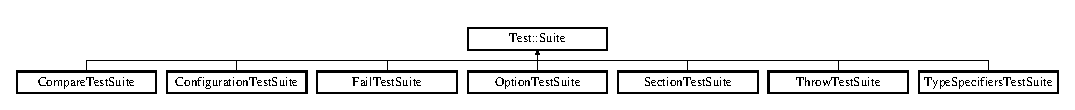
\includegraphics[height=1.025641cm]{class_test_1_1_suite}
\end{center}
\end{figure}
\subsection*{Classes}
\begin{DoxyCompactItemize}
\item 
struct \hyperlink{struct_test_1_1_suite_1_1_do_run}{Do\+Run}
\item 
struct \hyperlink{struct_test_1_1_suite_1_1_exec_tests}{Exec\+Tests}
\item 
struct \hyperlink{struct_test_1_1_suite_1_1_sub_suite_tests}{Sub\+Suite\+Tests}
\item 
struct \hyperlink{struct_test_1_1_suite_1_1_sub_suite_time}{Sub\+Suite\+Time}
\item 
struct \hyperlink{struct_test_1_1_suite_1_1_suite_time}{Suite\+Time}
\end{DoxyCompactItemize}
\subsection*{Public Member Functions}
\begin{DoxyCompactItemize}
\item 
\hyperlink{class_test_1_1_suite_a8cb51a002cf4e675820f91fe03ec9117}{Suite} ()
\item 
virtual \hyperlink{class_test_1_1_suite_a7a62f450d1e6c86cd6058e1c457aa4b7}{$\sim$\+Suite} ()
\item 
void \hyperlink{class_test_1_1_suite_a0237b63fc694ecb133d023cf2d6ab271}{add} (std\+::auto\+\_\+ptr$<$ \hyperlink{class_test_1_1_suite}{Suite} $>$ suite)
\item 
bool \hyperlink{class_test_1_1_suite_ad17746e218da79c537bc9d21e389f570}{run} (\hyperlink{class_test_1_1_output}{Output} \&output, bool cont\+\_\+after\+\_\+fail=true)
\end{DoxyCompactItemize}
\subsection*{Protected Types}
\begin{DoxyCompactItemize}
\item 
typedef void(Suite\+::$\ast$ \hyperlink{class_test_1_1_suite_a87c40a9c763fc3221bee0e70c431038f}{Func}) ()
\end{DoxyCompactItemize}
\subsection*{Protected Member Functions}
\begin{DoxyCompactItemize}
\item 
bool {\bfseries continue\+\_\+after\+\_\+failure} () const \hypertarget{class_test_1_1_suite_a76d5fbd5dafa352f6086f8ab0db3089f}{}\label{class_test_1_1_suite_a76d5fbd5dafa352f6086f8ab0db3089f}

\item 
virtual void \hyperlink{class_test_1_1_suite_afb4c733e6c46a011818bb02f2e8d5bb8}{setup} ()
\item 
virtual void \hyperlink{class_test_1_1_suite_a37d3595625cff09b8e43bf6c414ff610}{tear\+\_\+down} ()
\item 
void \hyperlink{class_test_1_1_suite_a11e542d1d45905b817b00c35660700b9}{register\+\_\+test} (\hyperlink{class_test_1_1_suite_a87c40a9c763fc3221bee0e70c431038f}{Func} func, const std\+::string \&name)
\item 
void \hyperlink{class_test_1_1_suite_a1851ad75aed6141a19a06eeeb0fe0d3c}{assertment} (\hyperlink{class_test_1_1_source}{Source} s)
\end{DoxyCompactItemize}
\subsection*{Friends}
\begin{DoxyCompactItemize}
\item 
struct {\bfseries Do\+Run}\hypertarget{class_test_1_1_suite_a843435d7ee79d23ed13e6eec5c7ac6bb}{}\label{class_test_1_1_suite_a843435d7ee79d23ed13e6eec5c7ac6bb}

\item 
struct {\bfseries Exec\+Tests}\hypertarget{class_test_1_1_suite_ab4730d33c1241aba407b71f8eafb7bcc}{}\label{class_test_1_1_suite_ab4730d33c1241aba407b71f8eafb7bcc}

\item 
struct {\bfseries Sub\+Suite\+Tests}\hypertarget{class_test_1_1_suite_a901d2d72cc93e087c94d99680f65fa8e}{}\label{class_test_1_1_suite_a901d2d72cc93e087c94d99680f65fa8e}

\item 
struct {\bfseries Sub\+Suite\+Time}\hypertarget{class_test_1_1_suite_a5933776e455e5bd9ad1d4a8b1c591aa2}{}\label{class_test_1_1_suite_a5933776e455e5bd9ad1d4a8b1c591aa2}

\end{DoxyCompactItemize}


\subsection{Detailed Description}
Unit testing suite. 

Base class for all suites. Derive from this class to create own test suites.

Test functions in derived classes are registered as tests using the \hyperlink{cpptest-suite_8h_abe8c3e0a2cf3893ebc1c265264ed9cb8}{T\+E\+S\+T\+\_\+\+A\+D\+D(func)}. Testing is started by \hyperlink{class_test_1_1_suite_ad17746e218da79c537bc9d21e389f570}{run()}. Note that suites may be embedded in other suites using \hyperlink{class_test_1_1_suite_a0237b63fc694ecb133d023cf2d6ab271}{add()}. 

Definition at line 52 of file cpptest-\/suite.\+h.



\subsection{Member Typedef Documentation}
\index{Test\+::\+Suite@{Test\+::\+Suite}!Func@{Func}}
\index{Func@{Func}!Test\+::\+Suite@{Test\+::\+Suite}}
\subsubsection[{\texorpdfstring{Func}{Func}}]{\setlength{\rightskip}{0pt plus 5cm}typedef void(Suite\+::$\ast$ Test\+::\+Suite\+::\+Func) ()\hspace{0.3cm}{\ttfamily [protected]}}\hypertarget{class_test_1_1_suite_a87c40a9c763fc3221bee0e70c431038f}{}\label{class_test_1_1_suite_a87c40a9c763fc3221bee0e70c431038f}
Pointer to a test function. 

Definition at line 65 of file cpptest-\/suite.\+h.



\subsection{Constructor \& Destructor Documentation}
\index{Test\+::\+Suite@{Test\+::\+Suite}!Suite@{Suite}}
\index{Suite@{Suite}!Test\+::\+Suite@{Test\+::\+Suite}}
\subsubsection[{\texorpdfstring{Suite()}{Suite()}}]{\setlength{\rightskip}{0pt plus 5cm}Test\+::\+Suite\+::\+Suite (
\begin{DoxyParamCaption}
{}
\end{DoxyParamCaption}
)}\hypertarget{class_test_1_1_suite_a8cb51a002cf4e675820f91fe03ec9117}{}\label{class_test_1_1_suite_a8cb51a002cf4e675820f91fe03ec9117}
Constructs an empty test suite. 

Definition at line 63 of file suite.\+cpp.

\index{Test\+::\+Suite@{Test\+::\+Suite}!````~Suite@{$\sim$\+Suite}}
\index{````~Suite@{$\sim$\+Suite}!Test\+::\+Suite@{Test\+::\+Suite}}
\subsubsection[{\texorpdfstring{$\sim$\+Suite()}{~Suite()}}]{\setlength{\rightskip}{0pt plus 5cm}Test\+::\+Suite\+::$\sim$\+Suite (
\begin{DoxyParamCaption}
{}
\end{DoxyParamCaption}
)\hspace{0.3cm}{\ttfamily [virtual]}}\hypertarget{class_test_1_1_suite_a7a62f450d1e6c86cd6058e1c457aa4b7}{}\label{class_test_1_1_suite_a7a62f450d1e6c86cd6058e1c457aa4b7}
Destroys this suite object. 

Definition at line 71 of file suite.\+cpp.



\subsection{Member Function Documentation}
\index{Test\+::\+Suite@{Test\+::\+Suite}!add@{add}}
\index{add@{add}!Test\+::\+Suite@{Test\+::\+Suite}}
\subsubsection[{\texorpdfstring{add(std\+::auto\+\_\+ptr$<$ Suite $>$ suite)}{add(std::auto_ptr< Suite > suite)}}]{\setlength{\rightskip}{0pt plus 5cm}void Test\+::\+Suite\+::add (
\begin{DoxyParamCaption}
\item[{std\+::auto\+\_\+ptr$<$ {\bf Suite} $>$}]{suite}
\end{DoxyParamCaption}
)}\hypertarget{class_test_1_1_suite_a0237b63fc694ecb133d023cf2d6ab271}{}\label{class_test_1_1_suite_a0237b63fc694ecb133d023cf2d6ab271}
Adds a suite to this suite. Tests in added suites will be executed when \hyperlink{class_test_1_1_suite_ad17746e218da79c537bc9d21e389f570}{run()} of the top-\/level suite is called.


\begin{DoxyParams}{Parameters}
{\em suite} & Test suite to add. \\
\hline
\end{DoxyParams}


Definition at line 120 of file suite.\+cpp.

\index{Test\+::\+Suite@{Test\+::\+Suite}!assertment@{assertment}}
\index{assertment@{assertment}!Test\+::\+Suite@{Test\+::\+Suite}}
\subsubsection[{\texorpdfstring{assertment(\+Source s)}{assertment(Source s)}}]{\setlength{\rightskip}{0pt plus 5cm}void Test\+::\+Suite\+::assertment (
\begin{DoxyParamCaption}
\item[{{\bf Source}}]{s}
\end{DoxyParamCaption}
)\hspace{0.3cm}{\ttfamily [protected]}}\hypertarget{class_test_1_1_suite_a1851ad75aed6141a19a06eeeb0fe0d3c}{}\label{class_test_1_1_suite_a1851ad75aed6141a19a06eeeb0fe0d3c}
Issues an assertment to the output handler.

Do not call this function directly, use one of the available assertment macros instead, see \hyperlink{asserts}{Available asserts}.


\begin{DoxyParams}{Parameters}
{\em s} & Assert point information. \\
\hline
\end{DoxyParams}


Definition at line 152 of file suite.\+cpp.

\index{Test\+::\+Suite@{Test\+::\+Suite}!register\+\_\+test@{register\+\_\+test}}
\index{register\+\_\+test@{register\+\_\+test}!Test\+::\+Suite@{Test\+::\+Suite}}
\subsubsection[{\texorpdfstring{register\+\_\+test(\+Func func, const std\+::string \&name)}{register_test(Func func, const std::string &name)}}]{\setlength{\rightskip}{0pt plus 5cm}void Test\+::\+Suite\+::register\+\_\+test (
\begin{DoxyParamCaption}
\item[{{\bf Func}}]{func, }
\item[{const std\+::string \&}]{name}
\end{DoxyParamCaption}
)\hspace{0.3cm}{\ttfamily [protected]}}\hypertarget{class_test_1_1_suite_a11e542d1d45905b817b00c35660700b9}{}\label{class_test_1_1_suite_a11e542d1d45905b817b00c35660700b9}
Registers a test function.

{\bfseries Note\+:} Do not call this function directly, use the \hyperlink{cpptest-suite_8h_abe8c3e0a2cf3893ebc1c265264ed9cb8}{T\+E\+S\+T\+\_\+\+A\+D\+D(func)} macro instead.


\begin{DoxyParams}{Parameters}
{\em func} & Pointer to a test function. \\
\hline
{\em name} & Class and function name of the function. The format {\bfseries must} equal {\itshape class\+::func}. \\
\hline
\end{DoxyParams}


Definition at line 135 of file suite.\+cpp.

\index{Test\+::\+Suite@{Test\+::\+Suite}!run@{run}}
\index{run@{run}!Test\+::\+Suite@{Test\+::\+Suite}}
\subsubsection[{\texorpdfstring{run(\+Output \&output, bool cont\+\_\+after\+\_\+fail=true)}{run(Output &output, bool cont_after_fail=true)}}]{\setlength{\rightskip}{0pt plus 5cm}bool Test\+::\+Suite\+::run (
\begin{DoxyParamCaption}
\item[{{\bf Output} \&}]{output, }
\item[{bool}]{cont\+\_\+after\+\_\+fail = {\ttfamily true}}
\end{DoxyParamCaption}
)}\hypertarget{class_test_1_1_suite_ad17746e218da79c537bc9d21e389f570}{}\label{class_test_1_1_suite_ad17746e218da79c537bc9d21e389f570}
Starts the testing. All tests in this suite and embedded suites will be executed.


\begin{DoxyParams}{Parameters}
{\em output} & Progress report destination. \\
\hline
{\em cont\+\_\+after\+\_\+fail} & Continue functions despite failures.\\
\hline
\end{DoxyParams}
\begin{DoxyReturn}{Returns}
True if no test failed; false otherwise. 
\end{DoxyReturn}


Definition at line 85 of file suite.\+cpp.

\index{Test\+::\+Suite@{Test\+::\+Suite}!setup@{setup}}
\index{setup@{setup}!Test\+::\+Suite@{Test\+::\+Suite}}
\subsubsection[{\texorpdfstring{setup()}{setup()}}]{\setlength{\rightskip}{0pt plus 5cm}void Test\+::\+Suite\+::setup (
\begin{DoxyParamCaption}
{}
\end{DoxyParamCaption}
)\hspace{0.3cm}{\ttfamily [inline]}, {\ttfamily [protected]}, {\ttfamily [virtual]}}\hypertarget{class_test_1_1_suite_afb4c733e6c46a011818bb02f2e8d5bb8}{}\label{class_test_1_1_suite_afb4c733e6c46a011818bb02f2e8d5bb8}
Setups a test fixture. This function is called before each test, in this suite, is executed.

This function should be overloaded by derived classes to provide specialized behavior.

\begin{DoxySeeAlso}{See also}
\hyperlink{class_test_1_1_suite_a37d3595625cff09b8e43bf6c414ff610}{tear\+\_\+down()} 
\end{DoxySeeAlso}


Definition at line 69 of file cpptest-\/suite.\+h.

\index{Test\+::\+Suite@{Test\+::\+Suite}!tear\+\_\+down@{tear\+\_\+down}}
\index{tear\+\_\+down@{tear\+\_\+down}!Test\+::\+Suite@{Test\+::\+Suite}}
\subsubsection[{\texorpdfstring{tear\+\_\+down()}{tear_down()}}]{\setlength{\rightskip}{0pt plus 5cm}void Test\+::\+Suite\+::tear\+\_\+down (
\begin{DoxyParamCaption}
{}
\end{DoxyParamCaption}
)\hspace{0.3cm}{\ttfamily [inline]}, {\ttfamily [protected]}, {\ttfamily [virtual]}}\hypertarget{class_test_1_1_suite_a37d3595625cff09b8e43bf6c414ff610}{}\label{class_test_1_1_suite_a37d3595625cff09b8e43bf6c414ff610}
Tears down a test fixture. This function is called after each test, in this suite, have been executed.

This function should be overloaded by derived classes to provide specialized behavior.

\begin{DoxySeeAlso}{See also}
\hyperlink{class_test_1_1_suite_afb4c733e6c46a011818bb02f2e8d5bb8}{setup()} 
\end{DoxySeeAlso}


Definition at line 70 of file cpptest-\/suite.\+h.



The documentation for this class was generated from the following files\+:\begin{DoxyCompactItemize}
\item 
lib/cpptest-\/1.\+1.\+2/src/\hyperlink{cpptest-suite_8h}{cpptest-\/suite.\+h}\item 
lib/cpptest-\/1.\+1.\+2/src/suite.\+cpp\end{DoxyCompactItemize}

\hypertarget{struct_test_1_1_collector_output_1_1_suite_info}{}\section{Test\+:\+:Collector\+Output\+:\+:Suite\+Info Struct Reference}
\label{struct_test_1_1_collector_output_1_1_suite_info}\index{Test\+::\+Collector\+Output\+::\+Suite\+Info@{Test\+::\+Collector\+Output\+::\+Suite\+Info}}
\subsection*{Public Member Functions}
\begin{DoxyCompactItemize}
\item 
{\bfseries Suite\+Info} (const std\+::string \&name, int tests)\hypertarget{struct_test_1_1_collector_output_1_1_suite_info_a293cc820c5745fc786faf3b8e2ab9438}{}\label{struct_test_1_1_collector_output_1_1_suite_info_a293cc820c5745fc786faf3b8e2ab9438}

\end{DoxyCompactItemize}
\subsection*{Public Attributes}
\begin{DoxyCompactItemize}
\item 
std\+::string {\bfseries \+\_\+name}\hypertarget{struct_test_1_1_collector_output_1_1_suite_info_a55bdc93b43037cba310bfd69441a3f15}{}\label{struct_test_1_1_collector_output_1_1_suite_info_a55bdc93b43037cba310bfd69441a3f15}

\item 
int {\bfseries \+\_\+errors}\hypertarget{struct_test_1_1_collector_output_1_1_suite_info_aad064ab88ce0e898be5b01ae98898e0f}{}\label{struct_test_1_1_collector_output_1_1_suite_info_aad064ab88ce0e898be5b01ae98898e0f}

\item 
Tests {\bfseries \+\_\+tests}\hypertarget{struct_test_1_1_collector_output_1_1_suite_info_aeffb563714b2ba368e8c9cc92cb78091}{}\label{struct_test_1_1_collector_output_1_1_suite_info_aeffb563714b2ba368e8c9cc92cb78091}

\item 
\hyperlink{class_test_1_1_time}{Time} {\bfseries \+\_\+time}\hypertarget{struct_test_1_1_collector_output_1_1_suite_info_a50173eba0cbf1c9e77bb029809a4580e}{}\label{struct_test_1_1_collector_output_1_1_suite_info_a50173eba0cbf1c9e77bb029809a4580e}

\end{DoxyCompactItemize}


\subsection{Detailed Description}


Definition at line 79 of file cpptest-\/collectoroutput.\+h.



The documentation for this struct was generated from the following files\+:\begin{DoxyCompactItemize}
\item 
lib/cpptest-\/1.\+1.\+2/src/\hyperlink{cpptest-collectoroutput_8h}{cpptest-\/collectoroutput.\+h}\item 
lib/cpptest-\/1.\+1.\+2/src/collectoroutput.\+cpp\end{DoxyCompactItemize}

\hypertarget{struct_test_1_1_html_output_1_1_suite_row}{}\section{Test\+:\+:Html\+Output\+:\+:Suite\+Row Struct Reference}
\label{struct_test_1_1_html_output_1_1_suite_row}\index{Test\+::\+Html\+Output\+::\+Suite\+Row@{Test\+::\+Html\+Output\+::\+Suite\+Row}}
\subsection*{Public Member Functions}
\begin{DoxyCompactItemize}
\item 
{\bfseries Suite\+Row} (ostream \&os)\hypertarget{struct_test_1_1_html_output_1_1_suite_row_aaa5f27c2da8cbbcb935d3488d4e7c761}{}\label{struct_test_1_1_html_output_1_1_suite_row_aaa5f27c2da8cbbcb935d3488d4e7c761}

\item 
void {\bfseries operator()} (const \hyperlink{struct_test_1_1_collector_output_1_1_suite_info}{Suite\+Info} \&si)\hypertarget{struct_test_1_1_html_output_1_1_suite_row_a17a452a03a365411190d5da93b5db2d4}{}\label{struct_test_1_1_html_output_1_1_suite_row_a17a452a03a365411190d5da93b5db2d4}

\end{DoxyCompactItemize}
\subsection*{Public Attributes}
\begin{DoxyCompactItemize}
\item 
ostream \& {\bfseries \+\_\+os}\hypertarget{struct_test_1_1_html_output_1_1_suite_row_a9424ee9c56deece0df65799d32ab6498}{}\label{struct_test_1_1_html_output_1_1_suite_row_a9424ee9c56deece0df65799d32ab6498}

\end{DoxyCompactItemize}


\subsection{Detailed Description}


Definition at line 240 of file htmloutput.\+cpp.



The documentation for this struct was generated from the following file\+:\begin{DoxyCompactItemize}
\item 
lib/cpptest-\/1.\+1.\+2/src/htmloutput.\+cpp\end{DoxyCompactItemize}

\hypertarget{struct_test_1_1_html_output_1_1_suite_test_result}{}\section{Test\+:\+:Html\+Output\+:\+:Suite\+Test\+Result Struct Reference}
\label{struct_test_1_1_html_output_1_1_suite_test_result}\index{Test\+::\+Html\+Output\+::\+Suite\+Test\+Result@{Test\+::\+Html\+Output\+::\+Suite\+Test\+Result}}
\subsection*{Public Member Functions}
\begin{DoxyCompactItemize}
\item 
{\bfseries Suite\+Test\+Result} (ostream \&os)\hypertarget{struct_test_1_1_html_output_1_1_suite_test_result_a4bbe1cf91cbb03755cbe3256dccdfb04}{}\label{struct_test_1_1_html_output_1_1_suite_test_result_a4bbe1cf91cbb03755cbe3256dccdfb04}

\item 
void {\bfseries operator()} (const \hyperlink{struct_test_1_1_collector_output_1_1_suite_info}{Suite\+Info} \&si)\hypertarget{struct_test_1_1_html_output_1_1_suite_test_result_ab3b121595de56c1eb22ca49c60aeb1be}{}\label{struct_test_1_1_html_output_1_1_suite_test_result_ab3b121595de56c1eb22ca49c60aeb1be}

\end{DoxyCompactItemize}
\subsection*{Public Attributes}
\begin{DoxyCompactItemize}
\item 
ostream \& {\bfseries \+\_\+os}\hypertarget{struct_test_1_1_html_output_1_1_suite_test_result_ad7f03c32f297e7010f0a091fd7b722e8}{}\label{struct_test_1_1_html_output_1_1_suite_test_result_ad7f03c32f297e7010f0a091fd7b722e8}

\end{DoxyCompactItemize}


\subsection{Detailed Description}


Definition at line 370 of file htmloutput.\+cpp.



The documentation for this struct was generated from the following file\+:\begin{DoxyCompactItemize}
\item 
lib/cpptest-\/1.\+1.\+2/src/htmloutput.\+cpp\end{DoxyCompactItemize}

\hypertarget{struct_test_1_1_suite_1_1_suite_time}{}\section{Test\+:\+:Suite\+:\+:Suite\+Time Struct Reference}
\label{struct_test_1_1_suite_1_1_suite_time}\index{Test\+::\+Suite\+::\+Suite\+Time@{Test\+::\+Suite\+::\+Suite\+Time}}
\subsection*{Public Member Functions}
\begin{DoxyCompactItemize}
\item 
\hyperlink{class_test_1_1_time}{Time} {\bfseries operator()} (const \hyperlink{class_test_1_1_time}{Time} \&time, const Data \&data)\hypertarget{struct_test_1_1_suite_1_1_suite_time_a286496110a79cecb0fe3cc05d0a918a8}{}\label{struct_test_1_1_suite_1_1_suite_time_a286496110a79cecb0fe3cc05d0a918a8}

\end{DoxyCompactItemize}


\subsection{Detailed Description}


Definition at line 250 of file suite.\+cpp.



The documentation for this struct was generated from the following file\+:\begin{DoxyCompactItemize}
\item 
lib/cpptest-\/1.\+1.\+2/src/suite.\+cpp\end{DoxyCompactItemize}

\hypertarget{struct_test_1_1_collector_output_1_1_test_info}{}\section{Test\+:\+:Collector\+Output\+:\+:Test\+Info Struct Reference}
\label{struct_test_1_1_collector_output_1_1_test_info}\index{Test\+::\+Collector\+Output\+::\+Test\+Info@{Test\+::\+Collector\+Output\+::\+Test\+Info}}
\subsection*{Public Member Functions}
\begin{DoxyCompactItemize}
\item 
{\bfseries Test\+Info} (const std\+::string name)\hypertarget{struct_test_1_1_collector_output_1_1_test_info_acfd49728d424c2824effe37beb85de87}{}\label{struct_test_1_1_collector_output_1_1_test_info_acfd49728d424c2824effe37beb85de87}

\end{DoxyCompactItemize}
\subsection*{Public Attributes}
\begin{DoxyCompactItemize}
\item 
std\+::string {\bfseries \+\_\+name}\hypertarget{struct_test_1_1_collector_output_1_1_test_info_aa28d98e3ea65b4dda28fbb8c62817cf5}{}\label{struct_test_1_1_collector_output_1_1_test_info_aa28d98e3ea65b4dda28fbb8c62817cf5}

\item 
\hyperlink{class_test_1_1_time}{Time} {\bfseries \+\_\+time}\hypertarget{struct_test_1_1_collector_output_1_1_test_info_a59094663d5e7e2a7d896ce574ae6ef1b}{}\label{struct_test_1_1_collector_output_1_1_test_info_a59094663d5e7e2a7d896ce574ae6ef1b}

\item 
bool {\bfseries \+\_\+success}\+: 1\hypertarget{struct_test_1_1_collector_output_1_1_test_info_a99a6450e62566587a15c9ae9b7073ae7}{}\label{struct_test_1_1_collector_output_1_1_test_info_a99a6450e62566587a15c9ae9b7073ae7}

\item 
Sources {\bfseries \+\_\+sources}\hypertarget{struct_test_1_1_collector_output_1_1_test_info_a930eb868ea4e8fb30577967179c80d77}{}\label{struct_test_1_1_collector_output_1_1_test_info_a930eb868ea4e8fb30577967179c80d77}

\end{DoxyCompactItemize}


\subsection{Detailed Description}


Definition at line 66 of file cpptest-\/collectoroutput.\+h.



The documentation for this struct was generated from the following files\+:\begin{DoxyCompactItemize}
\item 
lib/cpptest-\/1.\+1.\+2/src/\hyperlink{cpptest-collectoroutput_8h}{cpptest-\/collectoroutput.\+h}\item 
lib/cpptest-\/1.\+1.\+2/src/collectoroutput.\+cpp\end{DoxyCompactItemize}

\hypertarget{struct_test_1_1_html_output_1_1_test_result}{}\section{Test\+:\+:Html\+Output\+:\+:Test\+Result Struct Reference}
\label{struct_test_1_1_html_output_1_1_test_result}\index{Test\+::\+Html\+Output\+::\+Test\+Result@{Test\+::\+Html\+Output\+::\+Test\+Result}}
\subsection*{Public Member Functions}
\begin{DoxyCompactItemize}
\item 
{\bfseries Test\+Result} (ostream \&os)\hypertarget{struct_test_1_1_html_output_1_1_test_result_a51b442100cb31dca7e2f25cc06757971}{}\label{struct_test_1_1_html_output_1_1_test_result_a51b442100cb31dca7e2f25cc06757971}

\item 
void {\bfseries operator()} (const \hyperlink{class_test_1_1_source}{Source} \&s)\hypertarget{struct_test_1_1_html_output_1_1_test_result_ab5aaddd39ccf7814f910f9a7a88505a2}{}\label{struct_test_1_1_html_output_1_1_test_result_ab5aaddd39ccf7814f910f9a7a88505a2}

\end{DoxyCompactItemize}
\subsection*{Public Attributes}
\begin{DoxyCompactItemize}
\item 
ostream \& {\bfseries \+\_\+os}\hypertarget{struct_test_1_1_html_output_1_1_test_result_a00fdad3da3ee095194fb25f127bd453b}{}\label{struct_test_1_1_html_output_1_1_test_result_a00fdad3da3ee095194fb25f127bd453b}

\end{DoxyCompactItemize}


\subsection{Detailed Description}


Definition at line 321 of file htmloutput.\+cpp.



The documentation for this struct was generated from the following file\+:\begin{DoxyCompactItemize}
\item 
lib/cpptest-\/1.\+1.\+2/src/htmloutput.\+cpp\end{DoxyCompactItemize}

\hypertarget{struct_test_1_1_html_output_1_1_test_result_all}{}\section{Test\+:\+:Html\+Output\+:\+:Test\+Result\+All Struct Reference}
\label{struct_test_1_1_html_output_1_1_test_result_all}\index{Test\+::\+Html\+Output\+::\+Test\+Result\+All@{Test\+::\+Html\+Output\+::\+Test\+Result\+All}}
\subsection*{Public Member Functions}
\begin{DoxyCompactItemize}
\item 
{\bfseries Test\+Result\+All} (ostream \&os)\hypertarget{struct_test_1_1_html_output_1_1_test_result_all_a592ec25b7410b62cd5ae6bc7eeebe64b}{}\label{struct_test_1_1_html_output_1_1_test_result_all_a592ec25b7410b62cd5ae6bc7eeebe64b}

\item 
void {\bfseries operator()} (const \hyperlink{struct_test_1_1_collector_output_1_1_test_info}{Test\+Info} \&ti)\hypertarget{struct_test_1_1_html_output_1_1_test_result_all_accebc340ecf96cc31657848029703e72}{}\label{struct_test_1_1_html_output_1_1_test_result_all_accebc340ecf96cc31657848029703e72}

\end{DoxyCompactItemize}
\subsection*{Public Attributes}
\begin{DoxyCompactItemize}
\item 
ostream \& {\bfseries \+\_\+os}\hypertarget{struct_test_1_1_html_output_1_1_test_result_all_a101d2548b8d3da81bb9e8e940435158f}{}\label{struct_test_1_1_html_output_1_1_test_result_all_a101d2548b8d3da81bb9e8e940435158f}

\end{DoxyCompactItemize}


\subsection{Detailed Description}


Definition at line 351 of file htmloutput.\+cpp.



The documentation for this struct was generated from the following file\+:\begin{DoxyCompactItemize}
\item 
lib/cpptest-\/1.\+1.\+2/src/htmloutput.\+cpp\end{DoxyCompactItemize}

\hypertarget{struct_test_1_1_html_output_1_1_test_row}{}\section{Test\+:\+:Html\+Output\+:\+:Test\+Row Struct Reference}
\label{struct_test_1_1_html_output_1_1_test_row}\index{Test\+::\+Html\+Output\+::\+Test\+Row@{Test\+::\+Html\+Output\+::\+Test\+Row}}
\subsection*{Public Member Functions}
\begin{DoxyCompactItemize}
\item 
{\bfseries Test\+Row} (ostream \&os, bool incl\+\_\+ok\+\_\+tests)\hypertarget{struct_test_1_1_html_output_1_1_test_row_a6b1fda89cb8b52c6dbc2e356c429e809}{}\label{struct_test_1_1_html_output_1_1_test_row_a6b1fda89cb8b52c6dbc2e356c429e809}

\item 
void {\bfseries operator()} (const \hyperlink{struct_test_1_1_collector_output_1_1_test_info}{Test\+Info} \&ti)\hypertarget{struct_test_1_1_html_output_1_1_test_row_a8d0aa0f0f3d5a9f56e6a1c4171956a17}{}\label{struct_test_1_1_html_output_1_1_test_row_a8d0aa0f0f3d5a9f56e6a1c4171956a17}

\end{DoxyCompactItemize}
\subsection*{Public Attributes}
\begin{DoxyCompactItemize}
\item 
bool {\bfseries \+\_\+incl\+\_\+ok\+\_\+tests}\hypertarget{struct_test_1_1_html_output_1_1_test_row_a098830d7a70b454924711182f03618da}{}\label{struct_test_1_1_html_output_1_1_test_row_a098830d7a70b454924711182f03618da}

\item 
ostream \& {\bfseries \+\_\+os}\hypertarget{struct_test_1_1_html_output_1_1_test_row_ad079cbad0cc1ca7e3033fd756fefb3d5}{}\label{struct_test_1_1_html_output_1_1_test_row_ad079cbad0cc1ca7e3033fd756fefb3d5}

\end{DoxyCompactItemize}


\subsection{Detailed Description}


Definition at line 265 of file htmloutput.\+cpp.



The documentation for this struct was generated from the following file\+:\begin{DoxyCompactItemize}
\item 
lib/cpptest-\/1.\+1.\+2/src/htmloutput.\+cpp\end{DoxyCompactItemize}

\hypertarget{struct_test_1_1_html_output_1_1_test_suite_row}{}\section{Test\+:\+:Html\+Output\+:\+:Test\+Suite\+Row Struct Reference}
\label{struct_test_1_1_html_output_1_1_test_suite_row}\index{Test\+::\+Html\+Output\+::\+Test\+Suite\+Row@{Test\+::\+Html\+Output\+::\+Test\+Suite\+Row}}
\subsection*{Public Member Functions}
\begin{DoxyCompactItemize}
\item 
{\bfseries Test\+Suite\+Row} (ostream \&os, bool incl\+\_\+ok\+\_\+tests)\hypertarget{struct_test_1_1_html_output_1_1_test_suite_row_a875f5d4cce18583a1bc85d172c4685f4}{}\label{struct_test_1_1_html_output_1_1_test_suite_row_a875f5d4cce18583a1bc85d172c4685f4}

\item 
void {\bfseries operator()} (const \hyperlink{struct_test_1_1_collector_output_1_1_suite_info}{Suite\+Info} \&si)\hypertarget{struct_test_1_1_html_output_1_1_test_suite_row_a11f6791bdfd956514d843cbe0646a0c0}{}\label{struct_test_1_1_html_output_1_1_test_suite_row_a11f6791bdfd956514d843cbe0646a0c0}

\end{DoxyCompactItemize}
\subsection*{Public Attributes}
\begin{DoxyCompactItemize}
\item 
bool {\bfseries \+\_\+incl\+\_\+ok\+\_\+tests}\hypertarget{struct_test_1_1_html_output_1_1_test_suite_row_ad6af18d9f22c23ecf195015cead69128}{}\label{struct_test_1_1_html_output_1_1_test_suite_row_ad6af18d9f22c23ecf195015cead69128}

\item 
ostream \& {\bfseries \+\_\+os}\hypertarget{struct_test_1_1_html_output_1_1_test_suite_row_a64359aaeb40719886258eeb8864c0c04}{}\label{struct_test_1_1_html_output_1_1_test_suite_row_a64359aaeb40719886258eeb8864c0c04}

\end{DoxyCompactItemize}


\subsection{Detailed Description}


Definition at line 294 of file htmloutput.\+cpp.



The documentation for this struct was generated from the following file\+:\begin{DoxyCompactItemize}
\item 
lib/cpptest-\/1.\+1.\+2/src/htmloutput.\+cpp\end{DoxyCompactItemize}

\hypertarget{class_test_1_1_text_output}{}\section{Test\+:\+:Text\+Output Class Reference}
\label{class_test_1_1_text_output}\index{Test\+::\+Text\+Output@{Test\+::\+Text\+Output}}


Text output handler that outputs to the a stream.  




{\ttfamily \#include $<$cpptest-\/textoutput.\+h$>$}

Inheritance diagram for Test\+:\+:Text\+Output\+:\begin{figure}[H]
\begin{center}
\leavevmode
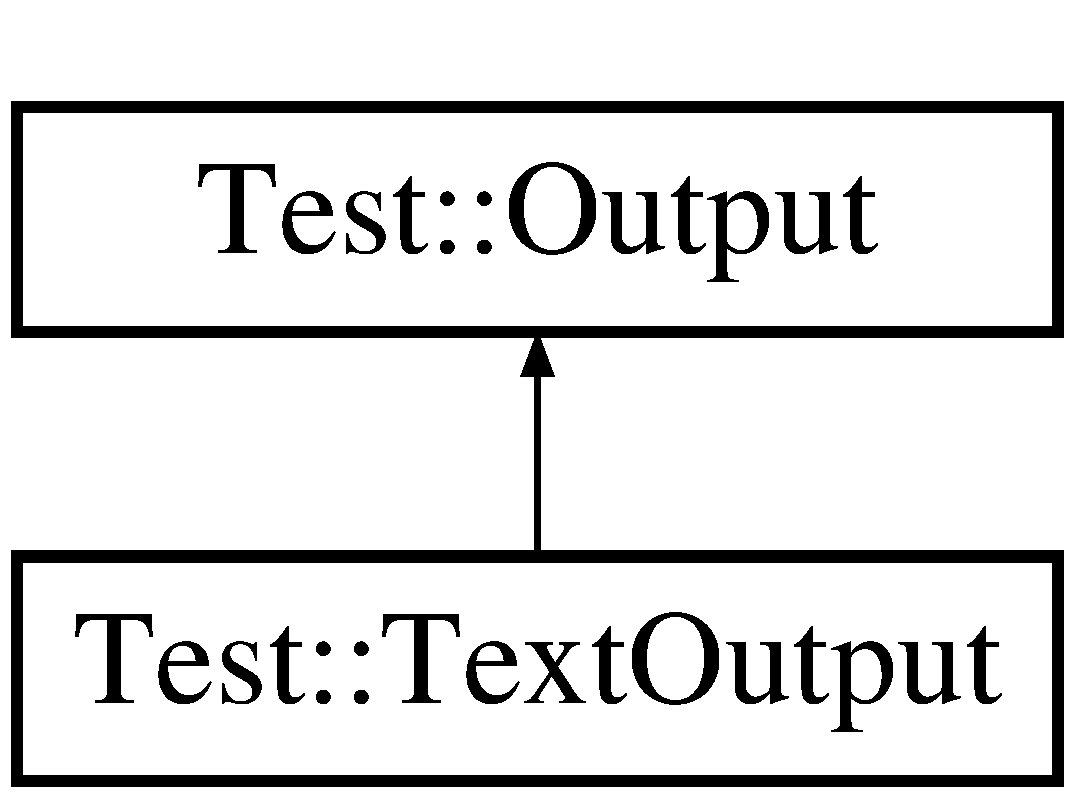
\includegraphics[height=2.000000cm]{class_test_1_1_text_output}
\end{center}
\end{figure}
\subsection*{Public Types}
\begin{DoxyCompactItemize}
\item 
enum \hyperlink{class_test_1_1_text_output_ae7b22c9458e6c566996bf4517c73feb1}{Mode} \{ \hyperlink{class_test_1_1_text_output_ae7b22c9458e6c566996bf4517c73feb1ae63930203459836dfc6e0939f92a9fb2}{Terse}, 
\hyperlink{class_test_1_1_text_output_ae7b22c9458e6c566996bf4517c73feb1a85dd6e42f6261a23fd504201f5cc2792}{Verbose}
 \}
\end{DoxyCompactItemize}
\subsection*{Public Member Functions}
\begin{DoxyCompactItemize}
\item 
\hyperlink{class_test_1_1_text_output_ab9bdd9b2d9b362ca5fb148b766ecdd02}{Text\+Output} (\hyperlink{class_test_1_1_text_output_ae7b22c9458e6c566996bf4517c73feb1}{Mode} mode, std\+::ostream \&stream=std\+::cout)
\item 
virtual void \hyperlink{class_test_1_1_text_output_ad139154d84e75aaaabed7b718b0ff106}{finished} (int tests, const \hyperlink{class_test_1_1_time}{Time} \&time)
\item 
virtual void \hyperlink{class_test_1_1_text_output_afa4d83846a506b7a26622711cbd69ad1}{suite\+\_\+start} (int tests, const std\+::string \&name)
\item 
virtual void \hyperlink{class_test_1_1_text_output_a7687ec2e87ccaa901e2b7d391937a71e}{suite\+\_\+end} (int tests, const std\+::string \&name, const \hyperlink{class_test_1_1_time}{Time} \&time)
\item 
virtual void \hyperlink{class_test_1_1_text_output_a61336a8ef939a9d826d4630da8020d72}{test\+\_\+end} (const std\+::string \&name, bool ok, const \hyperlink{class_test_1_1_time}{Time} \&time)
\item 
virtual void \hyperlink{class_test_1_1_text_output_a9acf66ddd0a5f584a86e5fbdd98e5f1a}{assertment} (const \hyperlink{class_test_1_1_source}{Source} \&s)
\end{DoxyCompactItemize}
\subsection*{Additional Inherited Members}


\subsection{Detailed Description}
Text output handler that outputs to the a stream. 

Test suite output handler that writes its information as text to a a stream. It it possible to select between two different operational modes that controls the detail level, see Mode. 

Definition at line 46 of file cpptest-\/textoutput.\+h.



\subsection{Member Enumeration Documentation}
\index{Test\+::\+Text\+Output@{Test\+::\+Text\+Output}!Mode@{Mode}}
\index{Mode@{Mode}!Test\+::\+Text\+Output@{Test\+::\+Text\+Output}}
\subsubsection[{\texorpdfstring{Mode}{Mode}}]{\setlength{\rightskip}{0pt plus 5cm}enum {\bf Test\+::\+Text\+Output\+::\+Mode}}\hypertarget{class_test_1_1_text_output_ae7b22c9458e6c566996bf4517c73feb1}{}\label{class_test_1_1_text_output_ae7b22c9458e6c566996bf4517c73feb1}
\hyperlink{class_test_1_1_output}{Output} mode. \begin{Desc}
\item[Enumerator]\par
\begin{description}
\index{Terse@{Terse}!Test\+::\+Text\+Output@{Test\+::\+Text\+Output}}\index{Test\+::\+Text\+Output@{Test\+::\+Text\+Output}!Terse@{Terse}}\item[{\em 
Terse\hypertarget{class_test_1_1_text_output_ae7b22c9458e6c566996bf4517c73feb1ae63930203459836dfc6e0939f92a9fb2}{}\label{class_test_1_1_text_output_ae7b22c9458e6c566996bf4517c73feb1ae63930203459836dfc6e0939f92a9fb2}
}]Terse output mode, which only shows the number of correct tests. \index{Verbose@{Verbose}!Test\+::\+Text\+Output@{Test\+::\+Text\+Output}}\index{Test\+::\+Text\+Output@{Test\+::\+Text\+Output}!Verbose@{Verbose}}\item[{\em 
Verbose\hypertarget{class_test_1_1_text_output_ae7b22c9458e6c566996bf4517c73feb1a85dd6e42f6261a23fd504201f5cc2792}{}\label{class_test_1_1_text_output_ae7b22c9458e6c566996bf4517c73feb1a85dd6e42f6261a23fd504201f5cc2792}
}]Verbose output mode, which also shows extended assert information for each test that failed. \end{description}
\end{Desc}


Definition at line 51 of file cpptest-\/textoutput.\+h.



\subsection{Constructor \& Destructor Documentation}
\index{Test\+::\+Text\+Output@{Test\+::\+Text\+Output}!Text\+Output@{Text\+Output}}
\index{Text\+Output@{Text\+Output}!Test\+::\+Text\+Output@{Test\+::\+Text\+Output}}
\subsubsection[{\texorpdfstring{Text\+Output(\+Mode mode, std\+::ostream \&stream=std\+::cout)}{TextOutput(Mode mode, std::ostream &stream=std::cout)}}]{\setlength{\rightskip}{0pt plus 5cm}Test\+::\+Text\+Output\+::\+Text\+Output (
\begin{DoxyParamCaption}
\item[{{\bf Mode}}]{mode, }
\item[{std\+::ostream \&}]{stream = {\ttfamily std\+:\+:cout}}
\end{DoxyParamCaption}
)}\hypertarget{class_test_1_1_text_output_ab9bdd9b2d9b362ca5fb148b766ecdd02}{}\label{class_test_1_1_text_output_ab9bdd9b2d9b362ca5fb148b766ecdd02}
Constructs a text output handler.


\begin{DoxyParams}{Parameters}
{\em mode} & \hyperlink{class_test_1_1_output}{Output} mode. \\
\hline
{\em stream} & Stream to output to. \\
\hline
\end{DoxyParams}


Definition at line 69 of file textoutput.\+cpp.



\subsection{Member Function Documentation}
\index{Test\+::\+Text\+Output@{Test\+::\+Text\+Output}!assertment@{assertment}}
\index{assertment@{assertment}!Test\+::\+Text\+Output@{Test\+::\+Text\+Output}}
\subsubsection[{\texorpdfstring{assertment(const Source \&s)}{assertment(const Source &s)}}]{\setlength{\rightskip}{0pt plus 5cm}void Test\+::\+Text\+Output\+::assertment (
\begin{DoxyParamCaption}
\item[{const {\bf Source} \&}]{s}
\end{DoxyParamCaption}
)\hspace{0.3cm}{\ttfamily [virtual]}}\hypertarget{class_test_1_1_text_output_a9acf66ddd0a5f584a86e5fbdd98e5f1a}{}\label{class_test_1_1_text_output_a9acf66ddd0a5f584a86e5fbdd98e5f1a}
Called when an assertment is issued.


\begin{DoxyParams}{Parameters}
{\em s} & Assert point information. \\
\hline
\end{DoxyParams}


Reimplemented from \hyperlink{class_test_1_1_output_a48c31f0baa7627d81939be840c9a7f65}{Test\+::\+Output}.



Definition at line 127 of file textoutput.\+cpp.

\index{Test\+::\+Text\+Output@{Test\+::\+Text\+Output}!finished@{finished}}
\index{finished@{finished}!Test\+::\+Text\+Output@{Test\+::\+Text\+Output}}
\subsubsection[{\texorpdfstring{finished(int tests, const Time \&time)}{finished(int tests, const Time &time)}}]{\setlength{\rightskip}{0pt plus 5cm}void Test\+::\+Text\+Output\+::finished (
\begin{DoxyParamCaption}
\item[{int}]{tests, }
\item[{const {\bf Time} \&}]{time}
\end{DoxyParamCaption}
)\hspace{0.3cm}{\ttfamily [virtual]}}\hypertarget{class_test_1_1_text_output_ad139154d84e75aaaabed7b718b0ff106}{}\label{class_test_1_1_text_output_ad139154d84e75aaaabed7b718b0ff106}
Called when testing is finished.


\begin{DoxyParams}{Parameters}
{\em tests} & Total number of tests in all suites. \\
\hline
{\em time} & Total elapsed time for all tests. \\
\hline
\end{DoxyParams}


Reimplemented from \hyperlink{class_test_1_1_output_aeff8af8326a8c54a38199f76837f860a}{Test\+::\+Output}.



Definition at line 76 of file textoutput.\+cpp.

\index{Test\+::\+Text\+Output@{Test\+::\+Text\+Output}!suite\+\_\+end@{suite\+\_\+end}}
\index{suite\+\_\+end@{suite\+\_\+end}!Test\+::\+Text\+Output@{Test\+::\+Text\+Output}}
\subsubsection[{\texorpdfstring{suite\+\_\+end(int tests, const std\+::string \&name, const Time \&time)}{suite_end(int tests, const std::string &name, const Time &time)}}]{\setlength{\rightskip}{0pt plus 5cm}void Test\+::\+Text\+Output\+::suite\+\_\+end (
\begin{DoxyParamCaption}
\item[{int}]{tests, }
\item[{const std\+::string \&}]{name, }
\item[{const {\bf Time} \&}]{time}
\end{DoxyParamCaption}
)\hspace{0.3cm}{\ttfamily [virtual]}}\hypertarget{class_test_1_1_text_output_a7687ec2e87ccaa901e2b7d391937a71e}{}\label{class_test_1_1_text_output_a7687ec2e87ccaa901e2b7d391937a71e}
Called when a suite is finished.


\begin{DoxyParams}{Parameters}
{\em tests} & Number of tests in this suite. \\
\hline
{\em name} & Name of the suite. \\
\hline
{\em time} & Total elapsed time for all tests in this suite. \\
\hline
\end{DoxyParams}


Reimplemented from \hyperlink{class_test_1_1_output_a6dbf4c0adb2bd4a7364c629179f788a6}{Test\+::\+Output}.



Definition at line 100 of file textoutput.\+cpp.

\index{Test\+::\+Text\+Output@{Test\+::\+Text\+Output}!suite\+\_\+start@{suite\+\_\+start}}
\index{suite\+\_\+start@{suite\+\_\+start}!Test\+::\+Text\+Output@{Test\+::\+Text\+Output}}
\subsubsection[{\texorpdfstring{suite\+\_\+start(int tests, const std\+::string \&name)}{suite_start(int tests, const std::string &name)}}]{\setlength{\rightskip}{0pt plus 5cm}void Test\+::\+Text\+Output\+::suite\+\_\+start (
\begin{DoxyParamCaption}
\item[{int}]{tests, }
\item[{const std\+::string \&}]{name}
\end{DoxyParamCaption}
)\hspace{0.3cm}{\ttfamily [virtual]}}\hypertarget{class_test_1_1_text_output_afa4d83846a506b7a26622711cbd69ad1}{}\label{class_test_1_1_text_output_afa4d83846a506b7a26622711cbd69ad1}
Called when a suite is entered.


\begin{DoxyParams}{Parameters}
{\em tests} & Number of tests in this suite. \\
\hline
{\em name} & Name of the suite. \\
\hline
\end{DoxyParams}


Reimplemented from \hyperlink{class_test_1_1_output_a7022c32c5a1577b10b93d3942746f17d}{Test\+::\+Output}.



Definition at line 84 of file textoutput.\+cpp.

\index{Test\+::\+Text\+Output@{Test\+::\+Text\+Output}!test\+\_\+end@{test\+\_\+end}}
\index{test\+\_\+end@{test\+\_\+end}!Test\+::\+Text\+Output@{Test\+::\+Text\+Output}}
\subsubsection[{\texorpdfstring{test\+\_\+end(const std\+::string \&name, bool ok, const Time \&time)}{test_end(const std::string &name, bool ok, const Time &time)}}]{\setlength{\rightskip}{0pt plus 5cm}void Test\+::\+Text\+Output\+::test\+\_\+end (
\begin{DoxyParamCaption}
\item[{const std\+::string \&}]{name, }
\item[{bool}]{ok, }
\item[{const {\bf Time} \&}]{time}
\end{DoxyParamCaption}
)\hspace{0.3cm}{\ttfamily [virtual]}}\hypertarget{class_test_1_1_text_output_a61336a8ef939a9d826d4630da8020d72}{}\label{class_test_1_1_text_output_a61336a8ef939a9d826d4630da8020d72}
Called when a test if finished, regardless if an assertment was issued.


\begin{DoxyParams}{Parameters}
{\em name} & Name of the test function. \\
\hline
{\em ok} & True if the test was successful; false otherwise. \\
\hline
{\em time} & Execution time. \\
\hline
\end{DoxyParams}


Reimplemented from \hyperlink{class_test_1_1_output_a3796943e3b56373492c957212a21454e}{Test\+::\+Output}.



Definition at line 117 of file textoutput.\+cpp.



The documentation for this class was generated from the following files\+:\begin{DoxyCompactItemize}
\item 
lib/cpptest-\/1.\+1.\+2/src/\hyperlink{cpptest-textoutput_8h}{cpptest-\/textoutput.\+h}\item 
lib/cpptest-\/1.\+1.\+2/src/textoutput.\+cpp\end{DoxyCompactItemize}

\hypertarget{class_throw_test_suite}{}\section{Throw\+Test\+Suite Class Reference}
\label{class_throw_test_suite}\index{Throw\+Test\+Suite@{Throw\+Test\+Suite}}
Inheritance diagram for Throw\+Test\+Suite\+:\begin{figure}[H]
\begin{center}
\leavevmode
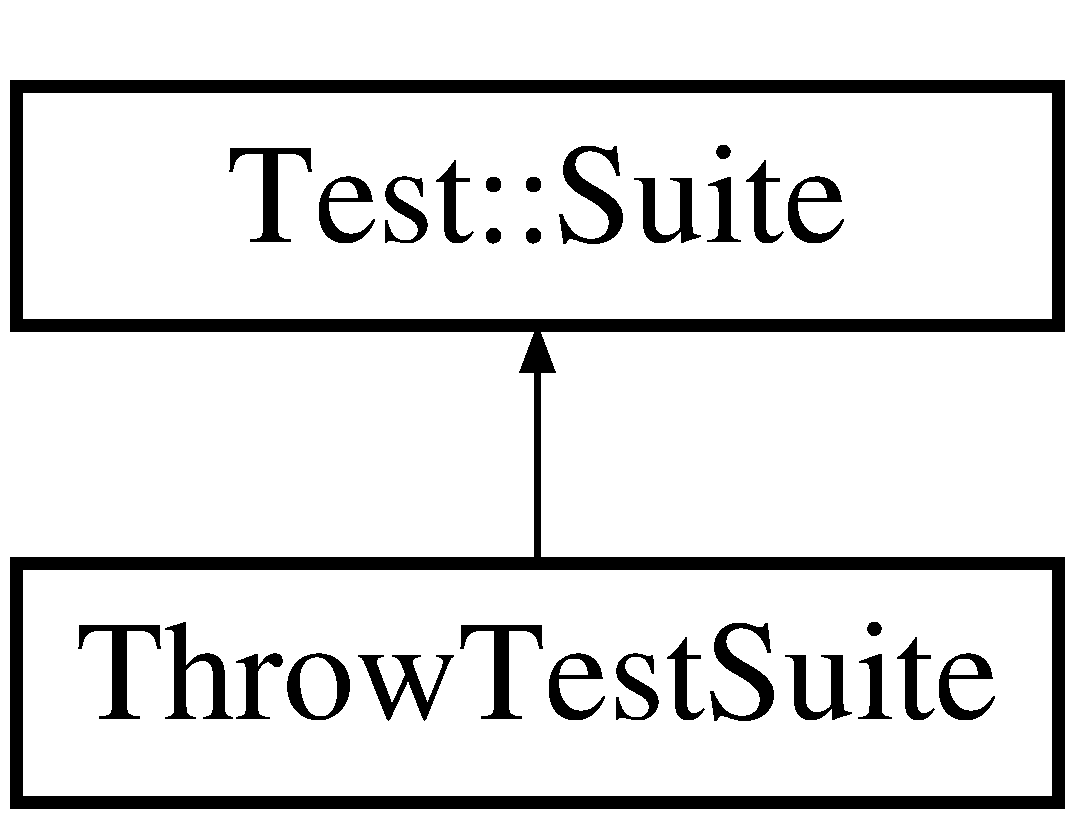
\includegraphics[height=2.000000cm]{class_throw_test_suite}
\end{center}
\end{figure}
\subsection*{Additional Inherited Members}


\subsection{Detailed Description}


Definition at line 106 of file mytest.\+cpp.



The documentation for this class was generated from the following file\+:\begin{DoxyCompactItemize}
\item 
lib/cpptest-\/1.\+1.\+2/test/mytest.\+cpp\end{DoxyCompactItemize}

\hypertarget{class_test_1_1_time}{}\section{Test\+:\+:Time Class Reference}
\label{class_test_1_1_time}\index{Test\+::\+Time@{Test\+::\+Time}}


Time representation.  




{\ttfamily \#include $<$cpptest-\/time.\+h$>$}

\subsection*{Public Member Functions}
\begin{DoxyCompactItemize}
\item 
\hyperlink{class_test_1_1_time_ae5c1089d2eb013c5b908ea95d924b733}{Time} ()
\item 
\hyperlink{class_test_1_1_time_afdc9c0556b8d71ecd8d621c2512154a5}{Time} (unsigned int sec, unsigned int usec)
\item 
unsigned int \hyperlink{class_test_1_1_time_a975b1bc3018cb82c5781edcbff7f32ff}{seconds} () const 
\item 
unsigned int \hyperlink{class_test_1_1_time_aee6b32be83b644a59ad89e539775ee54}{microseconds} () const 
\end{DoxyCompactItemize}
\subsection*{Static Public Member Functions}
\begin{DoxyCompactItemize}
\item 
static \hyperlink{class_test_1_1_time}{Time} \hyperlink{class_test_1_1_time_abb7a2480a7497c894994793da1a7b111}{current} ()
\end{DoxyCompactItemize}
\subsection*{Friends}
\begin{DoxyCompactItemize}
\item 
\hyperlink{class_test_1_1_time}{Time} {\bfseries operator+} (const \hyperlink{class_test_1_1_time}{Time} \&t1, const \hyperlink{class_test_1_1_time}{Time} \&t2)\hypertarget{class_test_1_1_time_ae2e555aa5b5c51e44b576d8baf48a2cd}{}\label{class_test_1_1_time_ae2e555aa5b5c51e44b576d8baf48a2cd}

\item 
\hyperlink{class_test_1_1_time}{Time} {\bfseries operator-\/} (const \hyperlink{class_test_1_1_time}{Time} \&t1, const \hyperlink{class_test_1_1_time}{Time} \&t2)\hypertarget{class_test_1_1_time_a09225563b0b317910b26c550ba74de64}{}\label{class_test_1_1_time_a09225563b0b317910b26c550ba74de64}

\item 
std\+::ostream \& {\bfseries operator$<$$<$} (std\+::ostream \&os, const \hyperlink{class_test_1_1_time}{Time} \&t)\hypertarget{class_test_1_1_time_a0287b008277738b9882ed96467e8b4f8}{}\label{class_test_1_1_time_a0287b008277738b9882ed96467e8b4f8}

\end{DoxyCompactItemize}
\subsection*{Related Functions}
(Note that these are not member functions.) \begin{DoxyCompactItemize}
\item 
\hyperlink{class_test_1_1_time}{Time} \hyperlink{class_test_1_1_time_a09225563b0b317910b26c550ba74de64}{operator-\/} (const \hyperlink{class_test_1_1_time}{Time} \&t1, const \hyperlink{class_test_1_1_time}{Time} \&t2)
\item 
\hyperlink{class_test_1_1_time}{Time} \hyperlink{class_test_1_1_time_ae2e555aa5b5c51e44b576d8baf48a2cd}{operator+} (const \hyperlink{class_test_1_1_time}{Time} \&t1, const \hyperlink{class_test_1_1_time}{Time} \&t2)
\item 
ostream \& \hyperlink{class_test_1_1_time_a5b08e472543c1992d2cadde99da4193b}{operator$<$$<$} (ostream \&os, const \hyperlink{class_test_1_1_time}{Time} \&t)
\end{DoxyCompactItemize}


\subsection{Detailed Description}
Time representation. 

Encapsulates a time value with microsecond resolution. It is possible to retrieve the current time, add and subtract time values, and output the time to an output stream. 

Definition at line 43 of file cpptest-\/time.\+h.



\subsection{Constructor \& Destructor Documentation}
\index{Test\+::\+Time@{Test\+::\+Time}!Time@{Time}}
\index{Time@{Time}!Test\+::\+Time@{Test\+::\+Time}}
\subsubsection[{\texorpdfstring{Time()}{Time()}}]{\setlength{\rightskip}{0pt plus 5cm}Test\+::\+Time\+::\+Time (
\begin{DoxyParamCaption}
{}
\end{DoxyParamCaption}
)}\hypertarget{class_test_1_1_time_ae5c1089d2eb013c5b908ea95d924b733}{}\label{class_test_1_1_time_ae5c1089d2eb013c5b908ea95d924b733}
Constructs a time object with zeroed time. 

Definition at line 56 of file time.\+cpp.

\index{Test\+::\+Time@{Test\+::\+Time}!Time@{Time}}
\index{Time@{Time}!Test\+::\+Time@{Test\+::\+Time}}
\subsubsection[{\texorpdfstring{Time(unsigned int sec, unsigned int usec)}{Time(unsigned int sec, unsigned int usec)}}]{\setlength{\rightskip}{0pt plus 5cm}Test\+::\+Time\+::\+Time (
\begin{DoxyParamCaption}
\item[{unsigned int}]{sec, }
\item[{unsigned int}]{usec}
\end{DoxyParamCaption}
)}\hypertarget{class_test_1_1_time_afdc9c0556b8d71ecd8d621c2512154a5}{}\label{class_test_1_1_time_afdc9c0556b8d71ecd8d621c2512154a5}
Constructs a time object.


\begin{DoxyParams}{Parameters}
{\em sec} & Seconds. \\
\hline
{\em usec} & Micro-\/seconds. \\
\hline
\end{DoxyParams}


Definition at line 66 of file time.\+cpp.



\subsection{Member Function Documentation}
\index{Test\+::\+Time@{Test\+::\+Time}!current@{current}}
\index{current@{current}!Test\+::\+Time@{Test\+::\+Time}}
\subsubsection[{\texorpdfstring{current()}{current()}}]{\setlength{\rightskip}{0pt plus 5cm}{\bf Time} Test\+::\+Time\+::current (
\begin{DoxyParamCaption}
{}
\end{DoxyParamCaption}
)\hspace{0.3cm}{\ttfamily [static]}}\hypertarget{class_test_1_1_time_abb7a2480a7497c894994793da1a7b111}{}\label{class_test_1_1_time_abb7a2480a7497c894994793da1a7b111}
\begin{DoxyReturn}{Returns}
The current time. 
\end{DoxyReturn}


Definition at line 90 of file time.\+cpp.

\index{Test\+::\+Time@{Test\+::\+Time}!microseconds@{microseconds}}
\index{microseconds@{microseconds}!Test\+::\+Time@{Test\+::\+Time}}
\subsubsection[{\texorpdfstring{microseconds() const }{microseconds() const }}]{\setlength{\rightskip}{0pt plus 5cm}unsigned int Test\+::\+Time\+::microseconds (
\begin{DoxyParamCaption}
{}
\end{DoxyParamCaption}
) const}\hypertarget{class_test_1_1_time_aee6b32be83b644a59ad89e539775ee54}{}\label{class_test_1_1_time_aee6b32be83b644a59ad89e539775ee54}
\begin{DoxyReturn}{Returns}
Micro-\/seconds. 
\end{DoxyReturn}


Definition at line 82 of file time.\+cpp.

\index{Test\+::\+Time@{Test\+::\+Time}!seconds@{seconds}}
\index{seconds@{seconds}!Test\+::\+Time@{Test\+::\+Time}}
\subsubsection[{\texorpdfstring{seconds() const }{seconds() const }}]{\setlength{\rightskip}{0pt plus 5cm}unsigned int Test\+::\+Time\+::seconds (
\begin{DoxyParamCaption}
{}
\end{DoxyParamCaption}
) const}\hypertarget{class_test_1_1_time_a975b1bc3018cb82c5781edcbff7f32ff}{}\label{class_test_1_1_time_a975b1bc3018cb82c5781edcbff7f32ff}
\begin{DoxyReturn}{Returns}
Seconds. 
\end{DoxyReturn}


Definition at line 74 of file time.\+cpp.



\subsection{Friends And Related Function Documentation}
\index{Test\+::\+Time@{Test\+::\+Time}!operator+@{operator+}}
\index{operator+@{operator+}!Test\+::\+Time@{Test\+::\+Time}}
\subsubsection[{\texorpdfstring{operator+(const Time \&t1, const Time \&t2)}{operator+(const Time &t1, const Time &t2)}}]{\setlength{\rightskip}{0pt plus 5cm}{\bf Time} operator+ (
\begin{DoxyParamCaption}
\item[{const {\bf Time} \&}]{t1, }
\item[{const {\bf Time} \&}]{t2}
\end{DoxyParamCaption}
)\hspace{0.3cm}{\ttfamily [related]}}\hypertarget{class_test_1_1_time_ae2e555aa5b5c51e44b576d8baf48a2cd}{}\label{class_test_1_1_time_ae2e555aa5b5c51e44b576d8baf48a2cd}
Adds two time values.


\begin{DoxyParams}{Parameters}
{\em t1} & Left-\/hand time. \\
\hline
{\em t2} & Right-\/hand time.\\
\hline
\end{DoxyParams}
\begin{DoxyReturn}{Returns}
Computed time value. 
\end{DoxyReturn}


Definition at line 136 of file time.\+cpp.

\index{Test\+::\+Time@{Test\+::\+Time}!operator-\/@{operator-\/}}
\index{operator-\/@{operator-\/}!Test\+::\+Time@{Test\+::\+Time}}
\subsubsection[{\texorpdfstring{operator-\/(const Time \&t1, const Time \&t2)}{operator-(const Time &t1, const Time &t2)}}]{\setlength{\rightskip}{0pt plus 5cm}{\bf Time} operator-\/ (
\begin{DoxyParamCaption}
\item[{const {\bf Time} \&}]{t1, }
\item[{const {\bf Time} \&}]{t2}
\end{DoxyParamCaption}
)\hspace{0.3cm}{\ttfamily [related]}}\hypertarget{class_test_1_1_time_a09225563b0b317910b26c550ba74de64}{}\label{class_test_1_1_time_a09225563b0b317910b26c550ba74de64}
Computes the time elapsed between two time values.


\begin{DoxyParams}{Parameters}
{\em t1} & Left-\/hand time, should be greater than {\itshape t2}. \\
\hline
{\em t2} & Right-\/hand time, should be less than {\itshape t1}.\\
\hline
\end{DoxyParams}
\begin{DoxyReturn}{Returns}
Computed time value. 
\end{DoxyReturn}


Definition at line 107 of file time.\+cpp.

\index{Test\+::\+Time@{Test\+::\+Time}!operator$<$$<$@{operator$<$$<$}}
\index{operator$<$$<$@{operator$<$$<$}!Test\+::\+Time@{Test\+::\+Time}}
\subsubsection[{\texorpdfstring{operator$<$$<$(ostream \&os, const Time \&t)}{operator<<(ostream &os, const Time &t)}}]{\setlength{\rightskip}{0pt plus 5cm}ostream \& operator$<$$<$ (
\begin{DoxyParamCaption}
\item[{ostream \&}]{os, }
\item[{const {\bf Time} \&}]{t}
\end{DoxyParamCaption}
)\hspace{0.3cm}{\ttfamily [related]}}\hypertarget{class_test_1_1_time_a5b08e472543c1992d2cadde99da4193b}{}\label{class_test_1_1_time_a5b08e472543c1992d2cadde99da4193b}
Outputs a time to an output stream.


\begin{DoxyParams}{Parameters}
{\em os} & \hyperlink{class_test_1_1_output}{Output} stream to write to. \\
\hline
{\em t} & Time to output.\\
\hline
\end{DoxyParams}
\begin{DoxyReturn}{Returns}
A reference to the given output stream. 
\end{DoxyReturn}


Definition at line 159 of file time.\+cpp.



The documentation for this class was generated from the following files\+:\begin{DoxyCompactItemize}
\item 
lib/cpptest-\/1.\+1.\+2/src/\hyperlink{cpptest-time_8h}{cpptest-\/time.\+h}\item 
lib/cpptest-\/1.\+1.\+2/src/time.\+cpp\end{DoxyCompactItemize}

\hypertarget{struct_test_1_1timeval}{}\section{Test\+:\+:timeval Struct Reference}
\label{struct_test_1_1timeval}\index{Test\+::timeval@{Test\+::timeval}}
\subsection*{Public Attributes}
\begin{DoxyCompactItemize}
\item 
long {\bfseries tv\+\_\+sec}\hypertarget{struct_test_1_1timeval_aca8cda492ba177e613667cc1d78e06d4}{}\label{struct_test_1_1timeval_aca8cda492ba177e613667cc1d78e06d4}

\item 
long {\bfseries tv\+\_\+usec}\hypertarget{struct_test_1_1timeval_a0d2f1f637ec31de63b2085cae7973e8a}{}\label{struct_test_1_1timeval_a0d2f1f637ec31de63b2085cae7973e8a}

\end{DoxyCompactItemize}


\subsection{Detailed Description}


Definition at line 40 of file missing.\+h.



The documentation for this struct was generated from the following file\+:\begin{DoxyCompactItemize}
\item 
lib/cpptest-\/1.\+1.\+2/src/missing.\+h\end{DoxyCompactItemize}

\hypertarget{class_config_manager_1_1_type_specifier}{}\section{Config\+Manager\+:\+:Type\+Specifier$<$ T\+Value\+Type $>$ Class Template Reference}
\label{class_config_manager_1_1_type_specifier}\index{Config\+Manager\+::\+Type\+Specifier$<$ T\+Value\+Type $>$@{Config\+Manager\+::\+Type\+Specifier$<$ T\+Value\+Type $>$}}


{\ttfamily \#include $<$typespecifiers.\+h$>$}

\subsection*{Public Types}
\begin{DoxyCompactItemize}
\item 
typedef T\+Value\+Type \hyperlink{class_config_manager_1_1_type_specifier_a30331e624a3c4a1c18eb5b838e93acea}{Value\+Type}
\end{DoxyCompactItemize}
\subsection*{Public Member Functions}
\begin{DoxyCompactItemize}
\item 
\hyperlink{class_config_manager_1_1_type_specifier_a11763b8857f9d1d00e72f4376749ac62}{Type\+Specifier} ()
\item 
\hyperlink{class_config_manager_1_1_type_specifier_a30331e624a3c4a1c18eb5b838e93acea}{Value\+Type} \hyperlink{class_config_manager_1_1_type_specifier_a4298803c2b4c3ca21f0861572ae917a3}{From\+String} (const std\+::string \&data)
\item 
std\+::string \hyperlink{class_config_manager_1_1_type_specifier_ae674750fb5e002cbd524adf80bfb7bc7}{To\+String} (const \hyperlink{class_config_manager_1_1_type_specifier_a30331e624a3c4a1c18eb5b838e93acea}{Value\+Type} \&value)
\end{DoxyCompactItemize}


\subsection{Detailed Description}
\subsubsection*{template$<$typename T\+Value\+Type$>$\\*
class Config\+Manager\+::\+Type\+Specifier$<$ T\+Value\+Type $>$}

Trida realizujici prevod z textu do nejakoho typu a zpet. Tato trida slouzi pouze jako ukazka rozhrani, ktere musi Type\+Specifiery splnovat. 

Definition at line 35 of file typespecifiers.\+h.



\subsection{Member Typedef Documentation}
\index{Config\+Manager\+::\+Type\+Specifier@{Config\+Manager\+::\+Type\+Specifier}!Value\+Type@{Value\+Type}}
\index{Value\+Type@{Value\+Type}!Config\+Manager\+::\+Type\+Specifier@{Config\+Manager\+::\+Type\+Specifier}}
\subsubsection[{\texorpdfstring{Value\+Type}{ValueType}}]{\setlength{\rightskip}{0pt plus 5cm}template$<$typename T\+Value\+Type $>$ typedef T\+Value\+Type {\bf Config\+Manager\+::\+Type\+Specifier}$<$ T\+Value\+Type $>$\+::{\bf Value\+Type}}\hypertarget{class_config_manager_1_1_type_specifier_a30331e624a3c4a1c18eb5b838e93acea}{}\label{class_config_manager_1_1_type_specifier_a30331e624a3c4a1c18eb5b838e93acea}
Tato definice typu urcuje navratovy typ. 

Definition at line 41 of file typespecifiers.\+h.



\subsection{Constructor \& Destructor Documentation}
\index{Config\+Manager\+::\+Type\+Specifier@{Config\+Manager\+::\+Type\+Specifier}!Type\+Specifier@{Type\+Specifier}}
\index{Type\+Specifier@{Type\+Specifier}!Config\+Manager\+::\+Type\+Specifier@{Config\+Manager\+::\+Type\+Specifier}}
\subsubsection[{\texorpdfstring{Type\+Specifier()}{TypeSpecifier()}}]{\setlength{\rightskip}{0pt plus 5cm}template$<$typename T\+Value\+Type $>$ {\bf Config\+Manager\+::\+Type\+Specifier}$<$ T\+Value\+Type $>$\+::{\bf Type\+Specifier} (
\begin{DoxyParamCaption}
{}
\end{DoxyParamCaption}
)}\hypertarget{class_config_manager_1_1_type_specifier_a11763b8857f9d1d00e72f4376749ac62}{}\label{class_config_manager_1_1_type_specifier_a11763b8857f9d1d00e72f4376749ac62}
Vychozi konstruktor je zapotrebi v pripadech, jelikoz musi byt nektere tridy, ktere Type\+Specifiery obsahuji, default inicializovany. 

\subsection{Member Function Documentation}
\index{Config\+Manager\+::\+Type\+Specifier@{Config\+Manager\+::\+Type\+Specifier}!From\+String@{From\+String}}
\index{From\+String@{From\+String}!Config\+Manager\+::\+Type\+Specifier@{Config\+Manager\+::\+Type\+Specifier}}
\subsubsection[{\texorpdfstring{From\+String(const std\+::string \&data)}{FromString(const std::string &data)}}]{\setlength{\rightskip}{0pt plus 5cm}template$<$typename T\+Value\+Type $>$ {\bf Value\+Type} {\bf Config\+Manager\+::\+Type\+Specifier}$<$ T\+Value\+Type $>$\+::From\+String (
\begin{DoxyParamCaption}
\item[{const std\+::string \&}]{data}
\end{DoxyParamCaption}
)}\hypertarget{class_config_manager_1_1_type_specifier_a4298803c2b4c3ca21f0861572ae917a3}{}\label{class_config_manager_1_1_type_specifier_a4298803c2b4c3ca21f0861572ae917a3}
Metoda prevadejici text na vyslednou hodnotu. Muze vyhodit \hyperlink{class_config_manager_1_1_wrong_format_exception}{Wrong\+Format\+Exception} vyjimku. 
\begin{DoxyParams}{Parameters}
{\em data} & Vstupni data. \\
\hline
\end{DoxyParams}
\index{Config\+Manager\+::\+Type\+Specifier@{Config\+Manager\+::\+Type\+Specifier}!To\+String@{To\+String}}
\index{To\+String@{To\+String}!Config\+Manager\+::\+Type\+Specifier@{Config\+Manager\+::\+Type\+Specifier}}
\subsubsection[{\texorpdfstring{To\+String(const Value\+Type \&value)}{ToString(const ValueType &value)}}]{\setlength{\rightskip}{0pt plus 5cm}template$<$typename T\+Value\+Type $>$ std\+::string {\bf Config\+Manager\+::\+Type\+Specifier}$<$ T\+Value\+Type $>$\+::To\+String (
\begin{DoxyParamCaption}
\item[{const {\bf Value\+Type} \&}]{value}
\end{DoxyParamCaption}
)}\hypertarget{class_config_manager_1_1_type_specifier_ae674750fb5e002cbd524adf80bfb7bc7}{}\label{class_config_manager_1_1_type_specifier_ae674750fb5e002cbd524adf80bfb7bc7}
Metoda prevadejici nastavenou/zmenenou hodnotu zpet do textoveho formatu. Muze vyhodit \hyperlink{class_config_manager_1_1_wrong_format_exception}{Wrong\+Format\+Exception} vyjimku. 
\begin{DoxyParams}{Parameters}
{\em Hodnota} & preveditelna na string. \\
\hline
\end{DoxyParams}


The documentation for this class was generated from the following file\+:\begin{DoxyCompactItemize}
\item 
src/\+Config\+Manager/typespecifiers.\+h\end{DoxyCompactItemize}

\hypertarget{class_type_specifiers_test_suite}{}\section{Type\+Specifiers\+Test\+Suite Class Reference}
\label{class_type_specifiers_test_suite}\index{Type\+Specifiers\+Test\+Suite@{Type\+Specifiers\+Test\+Suite}}
Inheritance diagram for Type\+Specifiers\+Test\+Suite\+:\begin{figure}[H]
\begin{center}
\leavevmode
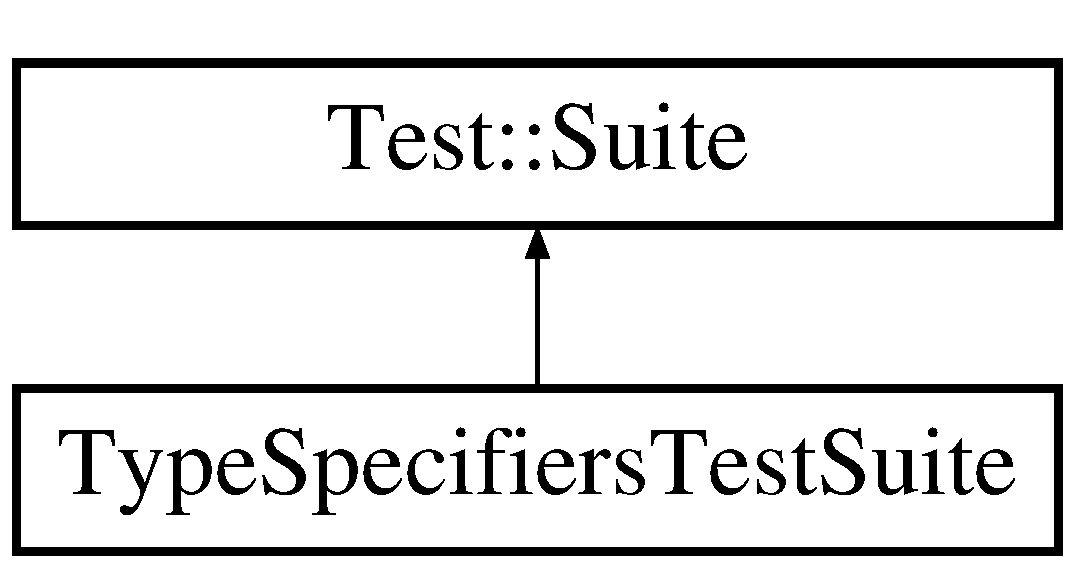
\includegraphics[height=2.000000cm]{class_type_specifiers_test_suite}
\end{center}
\end{figure}
\subsection*{Additional Inherited Members}


\subsection{Detailed Description}


Definition at line 87 of file tests.\+h.



The documentation for this class was generated from the following files\+:\begin{DoxyCompactItemize}
\item 
tests/tests.\+h\item 
tests/tests.\+cpp\end{DoxyCompactItemize}

\hypertarget{class_config_manager_1_1_unsigned_specifier}{}\section{Config\+Manager\+:\+:Unsigned\+Specifier Class Reference}
\label{class_config_manager_1_1_unsigned_specifier}\index{Config\+Manager\+::\+Unsigned\+Specifier@{Config\+Manager\+::\+Unsigned\+Specifier}}


{\ttfamily \#include $<$typespecifiers.\+h$>$}

Inheritance diagram for Config\+Manager\+:\+:Unsigned\+Specifier\+:\begin{figure}[H]
\begin{center}
\leavevmode
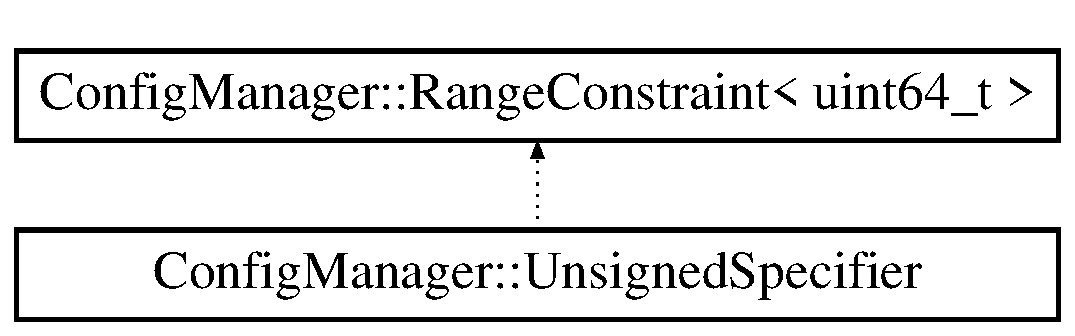
\includegraphics[height=2.000000cm]{class_config_manager_1_1_unsigned_specifier}
\end{center}
\end{figure}
\subsection*{Public Types}
\begin{DoxyCompactItemize}
\item 
typedef uint64\+\_\+t \hyperlink{class_config_manager_1_1_unsigned_specifier_aeaec69406d5a86486cb880750c3781e2}{Value\+Type}
\end{DoxyCompactItemize}
\subsection*{Public Member Functions}
\begin{DoxyCompactItemize}
\item 
\hyperlink{class_config_manager_1_1_unsigned_specifier_a123ab9e22e0757e91505222ca792ab56}{Unsigned\+Specifier} ()
\item 
\hyperlink{class_config_manager_1_1_unsigned_specifier_afb1ea2b4ea04fa083b22fc4ebdd763df}{Unsigned\+Specifier} (uint64\+\_\+t range\+\_\+start, uint64\+\_\+t range\+\_\+end)
\item 
\hyperlink{class_config_manager_1_1_unsigned_specifier_aeaec69406d5a86486cb880750c3781e2}{Value\+Type} \hyperlink{class_config_manager_1_1_unsigned_specifier_af4a11ae27e6ce3b4ab52995a48d37e9d}{From\+String} (const std\+::string \&data)
\item 
std\+::string \hyperlink{class_config_manager_1_1_unsigned_specifier_a10c19038f3a0fe8714dd689ab597e7d8}{To\+String} (\hyperlink{class_config_manager_1_1_unsigned_specifier_aeaec69406d5a86486cb880750c3781e2}{Value\+Type} value)
\end{DoxyCompactItemize}


\subsection{Detailed Description}
Trida realizujici prevod z textu do typu unsigned integer a zpet. 

Definition at line 137 of file typespecifiers.\+h.



\subsection{Member Typedef Documentation}
\index{Config\+Manager\+::\+Unsigned\+Specifier@{Config\+Manager\+::\+Unsigned\+Specifier}!Value\+Type@{Value\+Type}}
\index{Value\+Type@{Value\+Type}!Config\+Manager\+::\+Unsigned\+Specifier@{Config\+Manager\+::\+Unsigned\+Specifier}}
\subsubsection[{\texorpdfstring{Value\+Type}{ValueType}}]{\setlength{\rightskip}{0pt plus 5cm}typedef uint64\+\_\+t {\bf Config\+Manager\+::\+Unsigned\+Specifier\+::\+Value\+Type}}\hypertarget{class_config_manager_1_1_unsigned_specifier_aeaec69406d5a86486cb880750c3781e2}{}\label{class_config_manager_1_1_unsigned_specifier_aeaec69406d5a86486cb880750c3781e2}




Tato definice typu urcuje navratovy typ. 

Definition at line 143 of file typespecifiers.\+h.



\subsection{Constructor \& Destructor Documentation}
\index{Config\+Manager\+::\+Unsigned\+Specifier@{Config\+Manager\+::\+Unsigned\+Specifier}!Unsigned\+Specifier@{Unsigned\+Specifier}}
\index{Unsigned\+Specifier@{Unsigned\+Specifier}!Config\+Manager\+::\+Unsigned\+Specifier@{Config\+Manager\+::\+Unsigned\+Specifier}}
\subsubsection[{\texorpdfstring{Unsigned\+Specifier()}{UnsignedSpecifier()}}]{\setlength{\rightskip}{0pt plus 5cm}Config\+Manager\+::\+Unsigned\+Specifier\+::\+Unsigned\+Specifier (
\begin{DoxyParamCaption}
{}
\end{DoxyParamCaption}
)}\hypertarget{class_config_manager_1_1_unsigned_specifier_a123ab9e22e0757e91505222ca792ab56}{}\label{class_config_manager_1_1_unsigned_specifier_a123ab9e22e0757e91505222ca792ab56}




Konstruktor ktery neklade omezeni mezeni na rozsah hodnot. Rozsah hodnot je potom dan rozsahem zvoleneho typu. 

Definition at line 148 of file typespecifiers.\+cpp.

\index{Config\+Manager\+::\+Unsigned\+Specifier@{Config\+Manager\+::\+Unsigned\+Specifier}!Unsigned\+Specifier@{Unsigned\+Specifier}}
\index{Unsigned\+Specifier@{Unsigned\+Specifier}!Config\+Manager\+::\+Unsigned\+Specifier@{Config\+Manager\+::\+Unsigned\+Specifier}}
\subsubsection[{\texorpdfstring{Unsigned\+Specifier(uint64\+\_\+t range\+\_\+start, uint64\+\_\+t range\+\_\+end)}{UnsignedSpecifier(uint64_t range_start, uint64_t range_end)}}]{\setlength{\rightskip}{0pt plus 5cm}Config\+Manager\+::\+Unsigned\+Specifier\+::\+Unsigned\+Specifier (
\begin{DoxyParamCaption}
\item[{uint64\+\_\+t}]{range\+\_\+start, }
\item[{uint64\+\_\+t}]{range\+\_\+end}
\end{DoxyParamCaption}
)}\hypertarget{class_config_manager_1_1_unsigned_specifier_afb1ea2b4ea04fa083b22fc4ebdd763df}{}\label{class_config_manager_1_1_unsigned_specifier_afb1ea2b4ea04fa083b22fc4ebdd763df}






Definition at line 152 of file typespecifiers.\+cpp.



\subsection{Member Function Documentation}
\index{Config\+Manager\+::\+Unsigned\+Specifier@{Config\+Manager\+::\+Unsigned\+Specifier}!From\+String@{From\+String}}
\index{From\+String@{From\+String}!Config\+Manager\+::\+Unsigned\+Specifier@{Config\+Manager\+::\+Unsigned\+Specifier}}
\subsubsection[{\texorpdfstring{From\+String(const std\+::string \&data)}{FromString(const std::string &data)}}]{\setlength{\rightskip}{0pt plus 5cm}{\bf Unsigned\+Specifier\+::\+Value\+Type} Config\+Manager\+::\+Unsigned\+Specifier\+::\+From\+String (
\begin{DoxyParamCaption}
\item[{const std\+::string \&}]{data}
\end{DoxyParamCaption}
)}\hypertarget{class_config_manager_1_1_unsigned_specifier_af4a11ae27e6ce3b4ab52995a48d37e9d}{}\label{class_config_manager_1_1_unsigned_specifier_af4a11ae27e6ce3b4ab52995a48d37e9d}




Metoda prevadejici text na vyslednou hodnotu. Muze vyhodit \hyperlink{class_config_manager_1_1_wrong_format_exception}{Wrong\+Format\+Exception} vyjimku. 
\begin{DoxyParams}{Parameters}
{\em data} & Vstupni data. \\
\hline
\end{DoxyParams}


Definition at line 157 of file typespecifiers.\+cpp.

\index{Config\+Manager\+::\+Unsigned\+Specifier@{Config\+Manager\+::\+Unsigned\+Specifier}!To\+String@{To\+String}}
\index{To\+String@{To\+String}!Config\+Manager\+::\+Unsigned\+Specifier@{Config\+Manager\+::\+Unsigned\+Specifier}}
\subsubsection[{\texorpdfstring{To\+String(\+Value\+Type value)}{ToString(ValueType value)}}]{\setlength{\rightskip}{0pt plus 5cm}std\+::string Config\+Manager\+::\+Unsigned\+Specifier\+::\+To\+String (
\begin{DoxyParamCaption}
\item[{{\bf Unsigned\+Specifier\+::\+Value\+Type}}]{value}
\end{DoxyParamCaption}
)}\hypertarget{class_config_manager_1_1_unsigned_specifier_a10c19038f3a0fe8714dd689ab597e7d8}{}\label{class_config_manager_1_1_unsigned_specifier_a10c19038f3a0fe8714dd689ab597e7d8}






Definition at line 185 of file typespecifiers.\+cpp.



The documentation for this class was generated from the following files\+:\begin{DoxyCompactItemize}
\item 
E\+:/\+I\+N\+F\+O\+R\+M\+A\+T\+I\+K\+A/doporucene\+Postupy/uloha4/repos/src/\+Config\+Manager/typespecifiers.\+h\item 
E\+:/\+I\+N\+F\+O\+R\+M\+A\+T\+I\+K\+A/doporucene\+Postupy/uloha4/repos/src/\+Config\+Manager/typespecifiers.\+cpp\end{DoxyCompactItemize}

\hypertarget{class_config_manager_1_1_wrong_format_exception}{}\section{Config\+Manager\+:\+:Wrong\+Format\+Exception Class Reference}
\label{class_config_manager_1_1_wrong_format_exception}\index{Config\+Manager\+::\+Wrong\+Format\+Exception@{Config\+Manager\+::\+Wrong\+Format\+Exception}}


{\ttfamily \#include $<$exceptions.\+h$>$}

Inheritance diagram for Config\+Manager\+:\+:Wrong\+Format\+Exception\+:\begin{figure}[H]
\begin{center}
\leavevmode
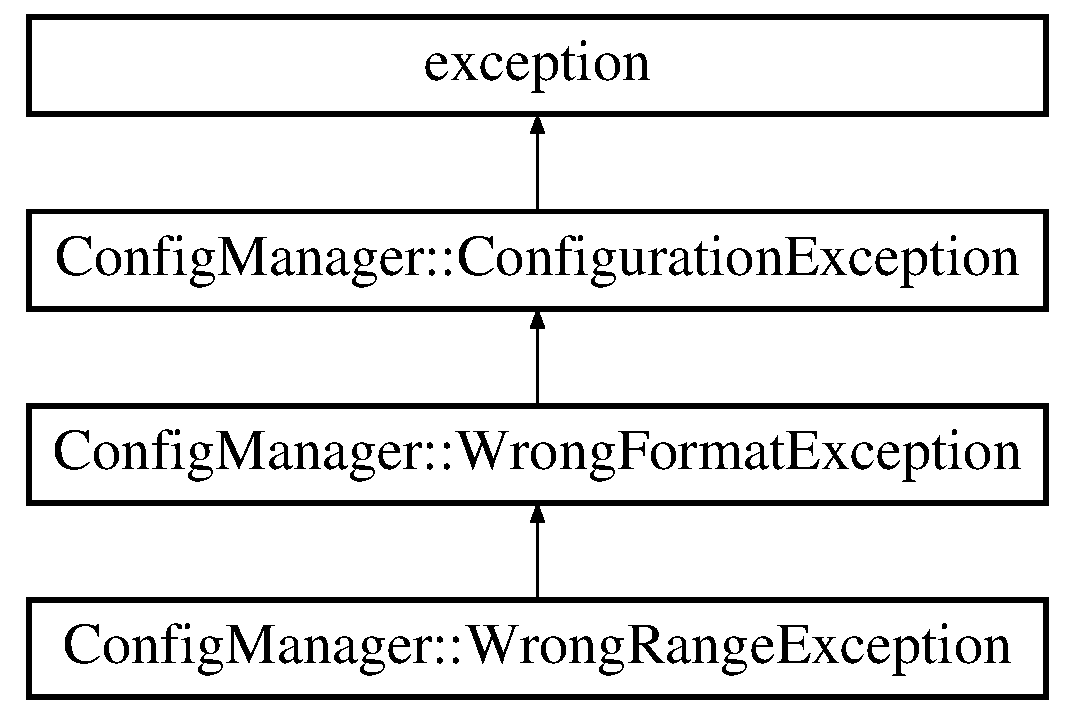
\includegraphics[height=4.000000cm]{class_config_manager_1_1_wrong_format_exception}
\end{center}
\end{figure}
\subsection*{Protected Member Functions}
\begin{DoxyCompactItemize}
\item 
{\bfseries Wrong\+Format\+Exception} (const char $\ast$message)\hypertarget{class_config_manager_1_1_wrong_format_exception_aa38389d999dd1c463fb887a36980b7ce}{}\label{class_config_manager_1_1_wrong_format_exception_aa38389d999dd1c463fb887a36980b7ce}

\end{DoxyCompactItemize}
\subsection*{Additional Inherited Members}


\subsection{Detailed Description}
Spatny format vstupnich dat (pro option). 

Definition at line 52 of file exceptions.\+h.



The documentation for this class was generated from the following file\+:\begin{DoxyCompactItemize}
\item 
E\+:/\+I\+N\+F\+O\+R\+M\+A\+T\+I\+K\+A/doporucene\+Postupy/uloha4/repos/src/\+Config\+Manager/exceptions.\+h\end{DoxyCompactItemize}

\hypertarget{class_config_manager_1_1_wrong_range_exception}{}\section{Config\+Manager\+:\+:Wrong\+Range\+Exception Class Reference}
\label{class_config_manager_1_1_wrong_range_exception}\index{Config\+Manager\+::\+Wrong\+Range\+Exception@{Config\+Manager\+::\+Wrong\+Range\+Exception}}
Inheritance diagram for Config\+Manager\+:\+:Wrong\+Range\+Exception\+:\begin{figure}[H]
\begin{center}
\leavevmode
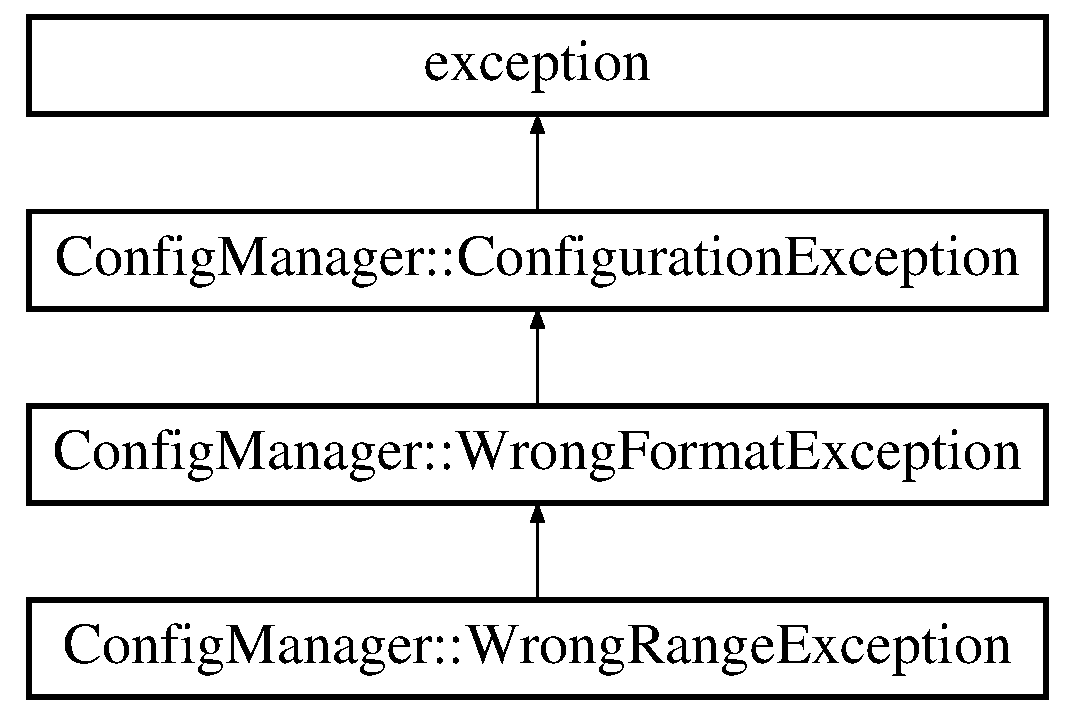
\includegraphics[height=4.000000cm]{class_config_manager_1_1_wrong_range_exception}
\end{center}
\end{figure}
\subsection*{Additional Inherited Members}


\subsection{Detailed Description}


Definition at line 47 of file exceptions.\+h.



The documentation for this class was generated from the following file\+:\begin{DoxyCompactItemize}
\item 
src/\+Config\+Manager/exceptions.\+h\end{DoxyCompactItemize}

\chapter{File Documentation}
\hypertarget{cpptest-assert_8h}{}\section{lib/cpptest-\/1.1.2/src/cpptest-\/assert.h File Reference}
\label{cpptest-assert_8h}\index{lib/cpptest-\/1.\+1.\+2/src/cpptest-\/assert.\+h@{lib/cpptest-\/1.\+1.\+2/src/cpptest-\/assert.\+h}}
{\ttfamily \#include $<$sstream$>$}\\*
\subsection*{Macros}
\begin{DoxyCompactItemize}
\item 
\#define \hyperlink{cpptest-assert_8h_a947ab44cc42369eb7cfe33f8a1e38e4b}{T\+E\+S\+T\+\_\+\+F\+A\+IL}(msg)
\item 
\#define \hyperlink{cpptest-assert_8h_ac7dd7b06eb85d9ad841d80cbf217b1f6}{T\+E\+S\+T\+\_\+\+A\+S\+S\+E\+RT}(expr) 	
\item 
\#define \hyperlink{cpptest-assert_8h_ac612ede938734f9c8d898e05818882fb}{T\+E\+S\+T\+\_\+\+A\+S\+S\+E\+R\+T\+\_\+\+M\+SG}(expr,  msg)
\item 
\#define \hyperlink{cpptest-assert_8h_ae281f4d973e657b11691a97551f17dd1}{T\+E\+S\+T\+\_\+\+A\+S\+S\+E\+R\+T\+\_\+\+E\+Q\+U\+A\+LS}(expected,  got)
\item 
\#define \hyperlink{cpptest-assert_8h_aa506d98e8a5fc575df0361906f7deef8}{T\+E\+S\+T\+\_\+\+A\+S\+S\+E\+R\+T\+\_\+\+E\+Q\+U\+A\+L\+S\+\_\+\+O\+BJ}(expected,  got)
\item 
\#define \hyperlink{cpptest-assert_8h_ab8e9ce729f96abe74b76d98f9568a59c}{T\+E\+S\+T\+\_\+\+A\+S\+S\+E\+R\+T\+\_\+\+E\+Q\+U\+A\+L\+S\+\_\+\+M\+SG}(expected,  got,  msg)
\item 
\#define \hyperlink{cpptest-assert_8h_a9583b1709f4b9dfb3ff2849bfec5c885}{T\+E\+S\+T\+\_\+\+A\+S\+S\+E\+R\+T\+\_\+\+D\+E\+L\+TA}(a,  b,  delta)
\item 
\#define \hyperlink{cpptest-assert_8h_afcd749452840bfde9be575ef22fcede0}{T\+E\+S\+T\+\_\+\+A\+S\+S\+E\+R\+T\+\_\+\+D\+E\+L\+T\+A\+\_\+\+M\+SG}(a,  b,  delta,  msg)
\item 
\#define \hyperlink{cpptest-assert_8h_a5174c5f93519d5726c8993b2f36d6ceb}{T\+E\+S\+T\+\_\+\+T\+H\+R\+O\+WS}(expr,  x)
\item 
\#define \hyperlink{cpptest-assert_8h_a1ce6abe9e9134ce993840a648673e0f2}{T\+E\+S\+T\+\_\+\+T\+H\+R\+O\+W\+S\+\_\+\+M\+SG}(expr,  x,  msg)
\item 
\#define \hyperlink{cpptest-assert_8h_a895af88056cd626a010136ac07b81d37}{T\+E\+S\+T\+\_\+\+T\+H\+R\+O\+W\+S\+\_\+\+A\+N\+Y\+T\+H\+I\+NG}(expr)
\item 
\#define \hyperlink{cpptest-assert_8h_a052597a8fd7dbc40ba350c735c4517c5}{T\+E\+S\+T\+\_\+\+T\+H\+R\+O\+W\+S\+\_\+\+A\+N\+Y\+T\+H\+I\+N\+G\+\_\+\+M\+SG}(expr,  msg)
\item 
\#define \hyperlink{cpptest-assert_8h_a885a5f6b6decac47414b4cc1a0a66425}{T\+E\+S\+T\+\_\+\+T\+H\+R\+O\+W\+S\+\_\+\+N\+O\+T\+H\+I\+NG}(expr)
\item 
\#define \hyperlink{cpptest-assert_8h_a758a47b613522a3d597c513786191ff9}{T\+E\+S\+T\+\_\+\+T\+H\+R\+O\+W\+S\+\_\+\+N\+O\+T\+H\+I\+N\+G\+\_\+\+M\+SG}(expr,  msg)
\end{DoxyCompactItemize}


\subsection{Macro Definition Documentation}
\index{cpptest-\/assert.\+h@{cpptest-\/assert.\+h}!T\+E\+S\+T\+\_\+\+A\+S\+S\+E\+RT@{T\+E\+S\+T\+\_\+\+A\+S\+S\+E\+RT}}
\index{T\+E\+S\+T\+\_\+\+A\+S\+S\+E\+RT@{T\+E\+S\+T\+\_\+\+A\+S\+S\+E\+RT}!cpptest-\/assert.\+h@{cpptest-\/assert.\+h}}
\subsubsection[{\texorpdfstring{T\+E\+S\+T\+\_\+\+A\+S\+S\+E\+RT}{TEST_ASSERT}}]{\setlength{\rightskip}{0pt plus 5cm}\#define T\+E\+S\+T\+\_\+\+A\+S\+S\+E\+RT(
\begin{DoxyParamCaption}
\item[{}]{expr}
\end{DoxyParamCaption}
)}\hypertarget{cpptest-assert_8h_ac7dd7b06eb85d9ad841d80cbf217b1f6}{}\label{cpptest-assert_8h_ac7dd7b06eb85d9ad841d80cbf217b1f6}
{\bfseries Value\+:}
\begin{DoxyCode}
\{                                                               \(\backslash\)
        if (!(expr))                                                \(\backslash\)
        \{                                                           \(\backslash\)
            assertment(::\hyperlink{class_test_1_1_source}{Test::Source}(\_\_FILE\_\_, \_\_LINE\_\_, #expr));  \(\backslash\)
            if (!continue\_after\_failure()) return;                  \(\backslash\)
        \}                                                           \(\backslash\)
    \}
\end{DoxyCode}
Verify an expression and issues an assertment if it fails.

Used in conjunction with \hyperlink{class_test_1_1_suite}{Test\+::\+Suite}.


\begin{DoxyParams}{Parameters}
{\em expr} & Expression to test.\\
\hline
\end{DoxyParams}
\begin{DoxySeeAlso}{See also}
\hyperlink{cpptest-assert_8h_ac612ede938734f9c8d898e05818882fb}{T\+E\+S\+T\+\_\+\+A\+S\+S\+E\+R\+T\+\_\+\+M\+S\+G(expr, msg)}
\end{DoxySeeAlso}
\begin{DoxyParagraph}{Example\+:}

\begin{DoxyCode}
1 void MySuite::test()
2 \{
3     int i;
4 
5     // ...
6 
7     TEST\_ASSERT(i == 13)
8 \}
\end{DoxyCode}

\end{DoxyParagraph}
For a description of all asserts, see \hyperlink{asserts}{Available asserts}. 

Definition at line 87 of file cpptest-\/assert.\+h.

\index{cpptest-\/assert.\+h@{cpptest-\/assert.\+h}!T\+E\+S\+T\+\_\+\+A\+S\+S\+E\+R\+T\+\_\+\+D\+E\+L\+TA@{T\+E\+S\+T\+\_\+\+A\+S\+S\+E\+R\+T\+\_\+\+D\+E\+L\+TA}}
\index{T\+E\+S\+T\+\_\+\+A\+S\+S\+E\+R\+T\+\_\+\+D\+E\+L\+TA@{T\+E\+S\+T\+\_\+\+A\+S\+S\+E\+R\+T\+\_\+\+D\+E\+L\+TA}!cpptest-\/assert.\+h@{cpptest-\/assert.\+h}}
\subsubsection[{\texorpdfstring{T\+E\+S\+T\+\_\+\+A\+S\+S\+E\+R\+T\+\_\+\+D\+E\+L\+TA}{TEST_ASSERT_DELTA}}]{\setlength{\rightskip}{0pt plus 5cm}\#define T\+E\+S\+T\+\_\+\+A\+S\+S\+E\+R\+T\+\_\+\+D\+E\+L\+TA(
\begin{DoxyParamCaption}
\item[{}]{a, }
\item[{}]{b, }
\item[{}]{delta}
\end{DoxyParamCaption}
)}\hypertarget{cpptest-assert_8h_a9583b1709f4b9dfb3ff2849bfec5c885}{}\label{cpptest-assert_8h_a9583b1709f4b9dfb3ff2849bfec5c885}
{\bfseries Value\+:}
\begin{DoxyCode}
\{                                                               \(\backslash\)
        if (((b) < (a) - (delta)) || ((b) > (a) + (delta)))         \(\backslash\)
        \{                                                           \(\backslash\)
            assertment(::\hyperlink{class_test_1_1_source}{Test::Source}(\_\_FILE\_\_, \_\_LINE\_\_,           \(\backslash\)
                       \textcolor{stringliteral}{"delta("} #a \textcolor{stringliteral}{", "} #b \textcolor{stringliteral}{", "} #delta \textcolor{stringliteral}{")"} ));      \(\backslash\)
            if (!continue\_after\_failure()) return;                  \(\backslash\)
        \}                                                           \(\backslash\)
    \}
\end{DoxyCode}
Verify that two expressions are equal up to a constant, issues an assertment if it fails.

Used in conjunction with \hyperlink{class_test_1_1_suite}{Test\+::\+Suite}.


\begin{DoxyParams}{Parameters}
{\em a} & First expression to test. \\
\hline
{\em b} & Second expression to test. \\
\hline
{\em delta} & Constant.\\
\hline
\end{DoxyParams}
\begin{DoxySeeAlso}{See also}
\hyperlink{cpptest-assert_8h_afcd749452840bfde9be575ef22fcede0}{T\+E\+S\+T\+\_\+\+A\+S\+S\+E\+R\+T\+\_\+\+D\+E\+L\+T\+A\+\_\+\+M\+S\+G(a, b, delta, msg)}
\end{DoxySeeAlso}
For a description of all asserts, see \hyperlink{asserts}{Available asserts}. 

Definition at line 216 of file cpptest-\/assert.\+h.

\index{cpptest-\/assert.\+h@{cpptest-\/assert.\+h}!T\+E\+S\+T\+\_\+\+A\+S\+S\+E\+R\+T\+\_\+\+D\+E\+L\+T\+A\+\_\+\+M\+SG@{T\+E\+S\+T\+\_\+\+A\+S\+S\+E\+R\+T\+\_\+\+D\+E\+L\+T\+A\+\_\+\+M\+SG}}
\index{T\+E\+S\+T\+\_\+\+A\+S\+S\+E\+R\+T\+\_\+\+D\+E\+L\+T\+A\+\_\+\+M\+SG@{T\+E\+S\+T\+\_\+\+A\+S\+S\+E\+R\+T\+\_\+\+D\+E\+L\+T\+A\+\_\+\+M\+SG}!cpptest-\/assert.\+h@{cpptest-\/assert.\+h}}
\subsubsection[{\texorpdfstring{T\+E\+S\+T\+\_\+\+A\+S\+S\+E\+R\+T\+\_\+\+D\+E\+L\+T\+A\+\_\+\+M\+SG}{TEST_ASSERT_DELTA_MSG}}]{\setlength{\rightskip}{0pt plus 5cm}\#define T\+E\+S\+T\+\_\+\+A\+S\+S\+E\+R\+T\+\_\+\+D\+E\+L\+T\+A\+\_\+\+M\+SG(
\begin{DoxyParamCaption}
\item[{}]{a, }
\item[{}]{b, }
\item[{}]{delta, }
\item[{}]{msg}
\end{DoxyParamCaption}
)}\hypertarget{cpptest-assert_8h_afcd749452840bfde9be575ef22fcede0}{}\label{cpptest-assert_8h_afcd749452840bfde9be575ef22fcede0}
{\bfseries Value\+:}
\begin{DoxyCode}
\{                                                               \(\backslash\)
        if (((b) < (a) - (delta)) || ((b) > (a) + (delta)))         \(\backslash\)
        \{                                                           \(\backslash\)
            assertment(::\hyperlink{class_test_1_1_source}{Test::Source}(\_\_FILE\_\_, \_\_LINE\_\_, msg));    \(\backslash\)
            if (!continue\_after\_failure()) return;                  \(\backslash\)
        \}                                                           \(\backslash\)
    \}
\end{DoxyCode}
Verify that two expressions are equal up to a constant, issues an assertment if it fails.

Used in conjunction with \hyperlink{class_test_1_1_suite}{Test\+::\+Suite}.


\begin{DoxyParams}{Parameters}
{\em a} & First expression to test. \\
\hline
{\em b} & Second expression to test. \\
\hline
{\em delta} & Constant. \\
\hline
{\em msg} & User message.\\
\hline
\end{DoxyParams}
\begin{DoxySeeAlso}{See also}
\hyperlink{cpptest-assert_8h_a9583b1709f4b9dfb3ff2849bfec5c885}{T\+E\+S\+T\+\_\+\+A\+S\+S\+E\+R\+T\+\_\+\+D\+E\+L\+T\+A(a, b, delta)}
\end{DoxySeeAlso}
For a description of all asserts, see \hyperlink{asserts}{Available asserts}. 

Definition at line 240 of file cpptest-\/assert.\+h.

\index{cpptest-\/assert.\+h@{cpptest-\/assert.\+h}!T\+E\+S\+T\+\_\+\+A\+S\+S\+E\+R\+T\+\_\+\+E\+Q\+U\+A\+LS@{T\+E\+S\+T\+\_\+\+A\+S\+S\+E\+R\+T\+\_\+\+E\+Q\+U\+A\+LS}}
\index{T\+E\+S\+T\+\_\+\+A\+S\+S\+E\+R\+T\+\_\+\+E\+Q\+U\+A\+LS@{T\+E\+S\+T\+\_\+\+A\+S\+S\+E\+R\+T\+\_\+\+E\+Q\+U\+A\+LS}!cpptest-\/assert.\+h@{cpptest-\/assert.\+h}}
\subsubsection[{\texorpdfstring{T\+E\+S\+T\+\_\+\+A\+S\+S\+E\+R\+T\+\_\+\+E\+Q\+U\+A\+LS}{TEST_ASSERT_EQUALS}}]{\setlength{\rightskip}{0pt plus 5cm}\#define T\+E\+S\+T\+\_\+\+A\+S\+S\+E\+R\+T\+\_\+\+E\+Q\+U\+A\+LS(
\begin{DoxyParamCaption}
\item[{}]{expected, }
\item[{}]{got}
\end{DoxyParamCaption}
)}\hypertarget{cpptest-assert_8h_ae281f4d973e657b11691a97551f17dd1}{}\label{cpptest-assert_8h_ae281f4d973e657b11691a97551f17dd1}
{\bfseries Value\+:}
\begin{DoxyCode}
\{                                                                   \(\backslash\)
        if (!((got) == (expected)))                                     \(\backslash\)
        \{                                                               \(\backslash\)
            std::stringstream tmpstream;                                \(\backslash\)
            tmpstream << \textcolor{stringliteral}{"Got "} << (got) << \textcolor{stringliteral}{", expected "} << (expected);\(\backslash\)
            assertment(::\hyperlink{class_test_1_1_source}{Test::Source}(\_\_FILE\_\_, \_\_LINE\_\_,               \(\backslash\)
                        tmpstream.str().c\_str()));                      \(\backslash\)
            if (!continue\_after\_failure()) return;                      \(\backslash\)
        \}                                                               \(\backslash\)
    \}
\end{DoxyCode}
Verify that two expressions are equal, issues an assertment if it fails. Requires the output operator ($<$$<$) to be defined for both expected and got.

If the output operator is not available, you should use \hyperlink{cpptest-assert_8h_aa506d98e8a5fc575df0361906f7deef8}{T\+E\+S\+T\+\_\+\+A\+S\+S\+E\+R\+T\+\_\+\+E\+Q\+U\+A\+L\+S\+\_\+\+O\+B\+J(expected, got)}.

Used in conjunction with \hyperlink{class_test_1_1_suite}{Test\+::\+Suite}.


\begin{DoxyParams}{Parameters}
{\em expected} & Expected value. \\
\hline
{\em got} & Value to test against expected value.\\
\hline
\end{DoxyParams}
\begin{DoxySeeAlso}{See also}
\hyperlink{cpptest-assert_8h_ab8e9ce729f96abe74b76d98f9568a59c}{T\+E\+S\+T\+\_\+\+A\+S\+S\+E\+R\+T\+\_\+\+E\+Q\+U\+A\+L\+S\+\_\+\+M\+S\+G(expected, got, msg)} 

\hyperlink{cpptest-assert_8h_aa506d98e8a5fc575df0361906f7deef8}{T\+E\+S\+T\+\_\+\+A\+S\+S\+E\+R\+T\+\_\+\+E\+Q\+U\+A\+L\+S\+\_\+\+O\+B\+J(expected, got)}
\end{DoxySeeAlso}
For a description of all asserts, see \hyperlink{asserts}{Available asserts}. 

Definition at line 133 of file cpptest-\/assert.\+h.

\index{cpptest-\/assert.\+h@{cpptest-\/assert.\+h}!T\+E\+S\+T\+\_\+\+A\+S\+S\+E\+R\+T\+\_\+\+E\+Q\+U\+A\+L\+S\+\_\+\+M\+SG@{T\+E\+S\+T\+\_\+\+A\+S\+S\+E\+R\+T\+\_\+\+E\+Q\+U\+A\+L\+S\+\_\+\+M\+SG}}
\index{T\+E\+S\+T\+\_\+\+A\+S\+S\+E\+R\+T\+\_\+\+E\+Q\+U\+A\+L\+S\+\_\+\+M\+SG@{T\+E\+S\+T\+\_\+\+A\+S\+S\+E\+R\+T\+\_\+\+E\+Q\+U\+A\+L\+S\+\_\+\+M\+SG}!cpptest-\/assert.\+h@{cpptest-\/assert.\+h}}
\subsubsection[{\texorpdfstring{T\+E\+S\+T\+\_\+\+A\+S\+S\+E\+R\+T\+\_\+\+E\+Q\+U\+A\+L\+S\+\_\+\+M\+SG}{TEST_ASSERT_EQUALS_MSG}}]{\setlength{\rightskip}{0pt plus 5cm}\#define T\+E\+S\+T\+\_\+\+A\+S\+S\+E\+R\+T\+\_\+\+E\+Q\+U\+A\+L\+S\+\_\+\+M\+SG(
\begin{DoxyParamCaption}
\item[{}]{expected, }
\item[{}]{got, }
\item[{}]{msg}
\end{DoxyParamCaption}
)}\hypertarget{cpptest-assert_8h_ab8e9ce729f96abe74b76d98f9568a59c}{}\label{cpptest-assert_8h_ab8e9ce729f96abe74b76d98f9568a59c}
{\bfseries Value\+:}
\begin{DoxyCode}
\{                                                                   \(\backslash\)
        if (!((got) == (expected)))                                     \(\backslash\)
        \{                                                               \(\backslash\)
            std::stringstream tmpstream;                                \(\backslash\)
            tmpstream << (msg) << \textcolor{stringliteral}{": "};                                 \(\backslash\)
            tmpstream << \textcolor{stringliteral}{"Got "} << (got) << \textcolor{stringliteral}{", expected "} << (expected);\(\backslash\)
            assertment(::\hyperlink{class_test_1_1_source}{Test::Source}(\_\_FILE\_\_, \_\_LINE\_\_,               \(\backslash\)
                        tmpstream.str().c\_str()));                      \(\backslash\)
            if (!continue\_after\_failure()) return;                      \(\backslash\)
        \}                                                               \(\backslash\)
    \}
\end{DoxyCode}
Verify that two expressions are equal, issues an assertment if it fails. The output operator ($<$$<$) must be defined for the object under test. If the output operator is not available, you should use \hyperlink{cpptest-assert_8h_aa506d98e8a5fc575df0361906f7deef8}{T\+E\+S\+T\+\_\+\+A\+S\+S\+E\+R\+T\+\_\+\+E\+Q\+U\+A\+L\+S\+\_\+\+O\+B\+J(expected, got)} instead.

Used in conjunction with \hyperlink{class_test_1_1_suite}{Test\+::\+Suite}.


\begin{DoxyParams}{Parameters}
{\em expected} & Expected value. \\
\hline
{\em got} & Value to test against expected value. \\
\hline
{\em msg} & User message to print out on failure.\\
\hline
\end{DoxyParams}
\begin{DoxySeeAlso}{See also}
\hyperlink{cpptest-assert_8h_ae281f4d973e657b11691a97551f17dd1}{T\+E\+S\+T\+\_\+\+A\+S\+S\+E\+R\+T\+\_\+\+E\+Q\+U\+A\+L\+S(expected, got)} 

\hyperlink{cpptest-assert_8h_aa506d98e8a5fc575df0361906f7deef8}{T\+E\+S\+T\+\_\+\+A\+S\+S\+E\+R\+T\+\_\+\+E\+Q\+U\+A\+L\+S\+\_\+\+O\+B\+J(expected, got)}
\end{DoxySeeAlso}
For a description of all asserts, see \hyperlink{asserts}{Available asserts}. 

Definition at line 190 of file cpptest-\/assert.\+h.

\index{cpptest-\/assert.\+h@{cpptest-\/assert.\+h}!T\+E\+S\+T\+\_\+\+A\+S\+S\+E\+R\+T\+\_\+\+E\+Q\+U\+A\+L\+S\+\_\+\+O\+BJ@{T\+E\+S\+T\+\_\+\+A\+S\+S\+E\+R\+T\+\_\+\+E\+Q\+U\+A\+L\+S\+\_\+\+O\+BJ}}
\index{T\+E\+S\+T\+\_\+\+A\+S\+S\+E\+R\+T\+\_\+\+E\+Q\+U\+A\+L\+S\+\_\+\+O\+BJ@{T\+E\+S\+T\+\_\+\+A\+S\+S\+E\+R\+T\+\_\+\+E\+Q\+U\+A\+L\+S\+\_\+\+O\+BJ}!cpptest-\/assert.\+h@{cpptest-\/assert.\+h}}
\subsubsection[{\texorpdfstring{T\+E\+S\+T\+\_\+\+A\+S\+S\+E\+R\+T\+\_\+\+E\+Q\+U\+A\+L\+S\+\_\+\+O\+BJ}{TEST_ASSERT_EQUALS_OBJ}}]{\setlength{\rightskip}{0pt plus 5cm}\#define T\+E\+S\+T\+\_\+\+A\+S\+S\+E\+R\+T\+\_\+\+E\+Q\+U\+A\+L\+S\+\_\+\+O\+BJ(
\begin{DoxyParamCaption}
\item[{}]{expected, }
\item[{}]{got}
\end{DoxyParamCaption}
)}\hypertarget{cpptest-assert_8h_aa506d98e8a5fc575df0361906f7deef8}{}\label{cpptest-assert_8h_aa506d98e8a5fc575df0361906f7deef8}
{\bfseries Value\+:}
\begin{DoxyCode}
\{                                                               \(\backslash\)
        if (!((got) == (expected)))                                 \(\backslash\)
        \{                                                           \(\backslash\)
            std::stringstream tmpstream;                            \(\backslash\)
            tmpstream << #expected << \textcolor{stringliteral}{" object not equal to "};      \(\backslash\)
            tmpstream << #got << \textcolor{stringliteral}{" object."};                        \(\backslash\)
            assertment(::\hyperlink{class_test_1_1_source}{Test::Source}(\_\_FILE\_\_, \_\_LINE\_\_,           \(\backslash\)
                        tmpstream.str().c\_str()));                  \(\backslash\)
            if (!continue\_after\_failure()) return;                  \(\backslash\)
        \}                                                           \(\backslash\)
    \}
\end{DoxyCode}
Verify that two expressions are equal, issues an assertment if it fails.

If the output operator is defined for the objects being compared you should use \hyperlink{cpptest-assert_8h_ae281f4d973e657b11691a97551f17dd1}{T\+E\+S\+T\+\_\+\+A\+S\+S\+E\+R\+T\+\_\+\+E\+Q\+U\+A\+L\+S(expected, got)} instead for more useful failure messages.

Used in conjunction with \hyperlink{class_test_1_1_suite}{Test\+::\+Suite}.


\begin{DoxyParams}{Parameters}
{\em expected} & Expected value. \\
\hline
{\em got} & Value to test against expected value.\\
\hline
\end{DoxyParams}
\begin{DoxySeeAlso}{See also}
\hyperlink{cpptest-assert_8h_ae281f4d973e657b11691a97551f17dd1}{T\+E\+S\+T\+\_\+\+A\+S\+S\+E\+R\+T\+\_\+\+E\+Q\+U\+A\+L\+S(expected, got)} 

\hyperlink{cpptest-assert_8h_ab8e9ce729f96abe74b76d98f9568a59c}{T\+E\+S\+T\+\_\+\+A\+S\+S\+E\+R\+T\+\_\+\+E\+Q\+U\+A\+L\+S\+\_\+\+M\+S\+G(expected, got, msg)}
\end{DoxySeeAlso}
For a description of all asserts, see \hyperlink{asserts}{Available asserts}. 

Definition at line 162 of file cpptest-\/assert.\+h.

\index{cpptest-\/assert.\+h@{cpptest-\/assert.\+h}!T\+E\+S\+T\+\_\+\+A\+S\+S\+E\+R\+T\+\_\+\+M\+SG@{T\+E\+S\+T\+\_\+\+A\+S\+S\+E\+R\+T\+\_\+\+M\+SG}}
\index{T\+E\+S\+T\+\_\+\+A\+S\+S\+E\+R\+T\+\_\+\+M\+SG@{T\+E\+S\+T\+\_\+\+A\+S\+S\+E\+R\+T\+\_\+\+M\+SG}!cpptest-\/assert.\+h@{cpptest-\/assert.\+h}}
\subsubsection[{\texorpdfstring{T\+E\+S\+T\+\_\+\+A\+S\+S\+E\+R\+T\+\_\+\+M\+SG}{TEST_ASSERT_MSG}}]{\setlength{\rightskip}{0pt plus 5cm}\#define T\+E\+S\+T\+\_\+\+A\+S\+S\+E\+R\+T\+\_\+\+M\+SG(
\begin{DoxyParamCaption}
\item[{}]{expr, }
\item[{}]{msg}
\end{DoxyParamCaption}
)}\hypertarget{cpptest-assert_8h_ac612ede938734f9c8d898e05818882fb}{}\label{cpptest-assert_8h_ac612ede938734f9c8d898e05818882fb}
{\bfseries Value\+:}
\begin{DoxyCode}
\{                                                               \(\backslash\)
        if (!(expr))                                                \(\backslash\)
        \{                                                           \(\backslash\)
            assertment(::\hyperlink{class_test_1_1_source}{Test::Source}(\_\_FILE\_\_, \_\_LINE\_\_, msg));    \(\backslash\)
            if (!continue\_after\_failure()) return;                  \(\backslash\)
        \}                                                           \(\backslash\)
    \}
\end{DoxyCode}
Verify an expression and issues an assertment if it fails.

Used in conjunction with \hyperlink{class_test_1_1_suite}{Test\+::\+Suite}.


\begin{DoxyParams}{Parameters}
{\em expr} & Expression to test. \\
\hline
{\em msg} & User message.\\
\hline
\end{DoxyParams}
\begin{DoxySeeAlso}{See also}
\hyperlink{cpptest-assert_8h_ac7dd7b06eb85d9ad841d80cbf217b1f6}{T\+E\+S\+T\+\_\+\+A\+S\+S\+E\+R\+T(expr)}
\end{DoxySeeAlso}
For a description of all asserts, see \hyperlink{asserts}{Available asserts}. 

Definition at line 107 of file cpptest-\/assert.\+h.

\index{cpptest-\/assert.\+h@{cpptest-\/assert.\+h}!T\+E\+S\+T\+\_\+\+F\+A\+IL@{T\+E\+S\+T\+\_\+\+F\+A\+IL}}
\index{T\+E\+S\+T\+\_\+\+F\+A\+IL@{T\+E\+S\+T\+\_\+\+F\+A\+IL}!cpptest-\/assert.\+h@{cpptest-\/assert.\+h}}
\subsubsection[{\texorpdfstring{T\+E\+S\+T\+\_\+\+F\+A\+IL}{TEST_FAIL}}]{\setlength{\rightskip}{0pt plus 5cm}\#define T\+E\+S\+T\+\_\+\+F\+A\+IL(
\begin{DoxyParamCaption}
\item[{}]{msg}
\end{DoxyParamCaption}
)}\hypertarget{cpptest-assert_8h_a947ab44cc42369eb7cfe33f8a1e38e4b}{}\label{cpptest-assert_8h_a947ab44cc42369eb7cfe33f8a1e38e4b}
{\bfseries Value\+:}
\begin{DoxyCode}
\{                                                               \(\backslash\)
        assertment(::\hyperlink{class_test_1_1_source}{Test::Source}(\_\_FILE\_\_, \_\_LINE\_\_, (msg) != 0 ? #msg : \textcolor{stringliteral}{""})); \(\backslash\)
        if (!continue\_after\_failure()) return;                      \(\backslash\)
    \}
\end{DoxyCode}
Unconditional failure.

Used in conjunction with \hyperlink{class_test_1_1_suite}{Test\+::\+Suite}.


\begin{DoxyParams}{Parameters}
{\em msg} & Provided message.\\
\hline
\end{DoxyParams}
\begin{DoxyParagraph}{Example\+:}

\begin{DoxyCode}
1 void MySuite::test()
2 \{
3     // ...
4 
5     switch (flag)
6     \{
7         // handling valid cases ...
8 
9         default:
10             TEST\_FAIL("This should not happen")
11     \}
12 \}
\end{DoxyCode}

\end{DoxyParagraph}
For a description of all asserts, see \hyperlink{asserts}{Available asserts}. 

Definition at line 59 of file cpptest-\/assert.\+h.

\index{cpptest-\/assert.\+h@{cpptest-\/assert.\+h}!T\+E\+S\+T\+\_\+\+T\+H\+R\+O\+WS@{T\+E\+S\+T\+\_\+\+T\+H\+R\+O\+WS}}
\index{T\+E\+S\+T\+\_\+\+T\+H\+R\+O\+WS@{T\+E\+S\+T\+\_\+\+T\+H\+R\+O\+WS}!cpptest-\/assert.\+h@{cpptest-\/assert.\+h}}
\subsubsection[{\texorpdfstring{T\+E\+S\+T\+\_\+\+T\+H\+R\+O\+WS}{TEST_THROWS}}]{\setlength{\rightskip}{0pt plus 5cm}\#define T\+E\+S\+T\+\_\+\+T\+H\+R\+O\+WS(
\begin{DoxyParamCaption}
\item[{}]{expr, }
\item[{}]{x}
\end{DoxyParamCaption}
)}\hypertarget{cpptest-assert_8h_a5174c5f93519d5726c8993b2f36d6ceb}{}\label{cpptest-assert_8h_a5174c5f93519d5726c8993b2f36d6ceb}
{\bfseries Value\+:}
\begin{DoxyCode}
\{                                                               \(\backslash\)
        bool \_\_expected = \textcolor{keyword}{false};                                    \(\backslash\)
        try \{ expr; \}                                               \(\backslash\)
        catch (x)           \{ \_\_expected = \textcolor{keyword}{true}; \}                  \(\backslash\)
        catch (...)         \{\}                                      \(\backslash\)
        if (!\_\_expected)                                            \(\backslash\)
        \{                                                           \(\backslash\)
            assertment(::\hyperlink{class_test_1_1_source}{Test::Source}(\_\_FILE\_\_, \_\_LINE\_\_, #expr));  \(\backslash\)
            if (!continue\_after\_failure()) return;                  \(\backslash\)
        \}                                                           \(\backslash\)
    \}
\end{DoxyCode}
Verify an expression and expects an exception in return. An assertment is issued if the exception is not thrown.

Used in conjunction with \hyperlink{class_test_1_1_suite}{Test\+::\+Suite}.


\begin{DoxyParams}{Parameters}
{\em expr} & Expression to test. \\
\hline
{\em x} & Expected exception.\\
\hline
\end{DoxyParams}
\begin{DoxySeeAlso}{See also}
\hyperlink{cpptest-assert_8h_a1ce6abe9e9134ce993840a648673e0f2}{T\+E\+S\+T\+\_\+\+T\+H\+R\+O\+W\+S\+\_\+\+M\+S\+G(expr, x, msg)}
\end{DoxySeeAlso}
For a description of all asserts, see \hyperlink{asserts}{Available asserts}. 

Definition at line 261 of file cpptest-\/assert.\+h.

\index{cpptest-\/assert.\+h@{cpptest-\/assert.\+h}!T\+E\+S\+T\+\_\+\+T\+H\+R\+O\+W\+S\+\_\+\+A\+N\+Y\+T\+H\+I\+NG@{T\+E\+S\+T\+\_\+\+T\+H\+R\+O\+W\+S\+\_\+\+A\+N\+Y\+T\+H\+I\+NG}}
\index{T\+E\+S\+T\+\_\+\+T\+H\+R\+O\+W\+S\+\_\+\+A\+N\+Y\+T\+H\+I\+NG@{T\+E\+S\+T\+\_\+\+T\+H\+R\+O\+W\+S\+\_\+\+A\+N\+Y\+T\+H\+I\+NG}!cpptest-\/assert.\+h@{cpptest-\/assert.\+h}}
\subsubsection[{\texorpdfstring{T\+E\+S\+T\+\_\+\+T\+H\+R\+O\+W\+S\+\_\+\+A\+N\+Y\+T\+H\+I\+NG}{TEST_THROWS_ANYTHING}}]{\setlength{\rightskip}{0pt plus 5cm}\#define T\+E\+S\+T\+\_\+\+T\+H\+R\+O\+W\+S\+\_\+\+A\+N\+Y\+T\+H\+I\+NG(
\begin{DoxyParamCaption}
\item[{}]{expr}
\end{DoxyParamCaption}
)}\hypertarget{cpptest-assert_8h_a895af88056cd626a010136ac07b81d37}{}\label{cpptest-assert_8h_a895af88056cd626a010136ac07b81d37}
{\bfseries Value\+:}
\begin{DoxyCode}
\{                                                               \(\backslash\)
        bool \_\_expected = \textcolor{keyword}{false};                                    \(\backslash\)
        try \{ expr; \}                                               \(\backslash\)
        catch (...) \{ \_\_expected = \textcolor{keyword}{true}; \}                          \(\backslash\)
        if (!\_\_expected)                                            \(\backslash\)
        \{                                                           \(\backslash\)
            assertment(::\hyperlink{class_test_1_1_source}{Test::Source}(\_\_FILE\_\_, \_\_LINE\_\_, #expr));  \(\backslash\)
            if (!continue\_after\_failure()) return;                  \(\backslash\)
        \}                                                           \(\backslash\)
    \}
\end{DoxyCode}
Verify an expression and expects any exception in return. An assertment is issued if no exception is thrown.

Used in conjunction with \hyperlink{class_test_1_1_suite}{Test\+::\+Suite}.


\begin{DoxyParams}{Parameters}
{\em expr} & Expression to test.\\
\hline
\end{DoxyParams}
\begin{DoxySeeAlso}{See also}
\hyperlink{cpptest-assert_8h_a052597a8fd7dbc40ba350c735c4517c5}{T\+E\+S\+T\+\_\+\+T\+H\+R\+O\+W\+S\+\_\+\+A\+N\+Y\+T\+H\+I\+N\+G\+\_\+\+M\+S\+G(expr, msg)}
\end{DoxySeeAlso}
For a description of all asserts, see \hyperlink{asserts}{Available asserts}. 

Definition at line 311 of file cpptest-\/assert.\+h.

\index{cpptest-\/assert.\+h@{cpptest-\/assert.\+h}!T\+E\+S\+T\+\_\+\+T\+H\+R\+O\+W\+S\+\_\+\+A\+N\+Y\+T\+H\+I\+N\+G\+\_\+\+M\+SG@{T\+E\+S\+T\+\_\+\+T\+H\+R\+O\+W\+S\+\_\+\+A\+N\+Y\+T\+H\+I\+N\+G\+\_\+\+M\+SG}}
\index{T\+E\+S\+T\+\_\+\+T\+H\+R\+O\+W\+S\+\_\+\+A\+N\+Y\+T\+H\+I\+N\+G\+\_\+\+M\+SG@{T\+E\+S\+T\+\_\+\+T\+H\+R\+O\+W\+S\+\_\+\+A\+N\+Y\+T\+H\+I\+N\+G\+\_\+\+M\+SG}!cpptest-\/assert.\+h@{cpptest-\/assert.\+h}}
\subsubsection[{\texorpdfstring{T\+E\+S\+T\+\_\+\+T\+H\+R\+O\+W\+S\+\_\+\+A\+N\+Y\+T\+H\+I\+N\+G\+\_\+\+M\+SG}{TEST_THROWS_ANYTHING_MSG}}]{\setlength{\rightskip}{0pt plus 5cm}\#define T\+E\+S\+T\+\_\+\+T\+H\+R\+O\+W\+S\+\_\+\+A\+N\+Y\+T\+H\+I\+N\+G\+\_\+\+M\+SG(
\begin{DoxyParamCaption}
\item[{}]{expr, }
\item[{}]{msg}
\end{DoxyParamCaption}
)}\hypertarget{cpptest-assert_8h_a052597a8fd7dbc40ba350c735c4517c5}{}\label{cpptest-assert_8h_a052597a8fd7dbc40ba350c735c4517c5}
{\bfseries Value\+:}
\begin{DoxyCode}
\{                                                               \(\backslash\)
        bool \_\_expected = \textcolor{keyword}{false};                                    \(\backslash\)
        try \{ expr; \}                                               \(\backslash\)
        catch (...) \{ \_\_expected = \textcolor{keyword}{true}; \}                          \(\backslash\)
        if (!\_\_expected)                                            \(\backslash\)
        \{                                                           \(\backslash\)
            assertment(::\hyperlink{class_test_1_1_source}{Test::Source}(\_\_FILE\_\_, \_\_LINE\_\_, msg));    \(\backslash\)
            if (!continue\_after\_failure()) return;                  \(\backslash\)
        \}                                                           \(\backslash\)
    \}
\end{DoxyCode}
Verify an expression and expects any exception in return. An assertment is issued if no exception is thrown.

Used in conjunction with \hyperlink{class_test_1_1_suite}{Test\+::\+Suite}.


\begin{DoxyParams}{Parameters}
{\em expr} & Expression to test. \\
\hline
{\em msg} & User message.\\
\hline
\end{DoxyParams}
\begin{DoxySeeAlso}{See also}
\hyperlink{cpptest-assert_8h_a895af88056cd626a010136ac07b81d37}{T\+E\+S\+T\+\_\+\+T\+H\+R\+O\+W\+S\+\_\+\+A\+N\+Y\+T\+H\+I\+N\+G(expr)}
\end{DoxySeeAlso}
For a description of all asserts, see \hyperlink{asserts}{Available asserts}. 

Definition at line 335 of file cpptest-\/assert.\+h.

\index{cpptest-\/assert.\+h@{cpptest-\/assert.\+h}!T\+E\+S\+T\+\_\+\+T\+H\+R\+O\+W\+S\+\_\+\+M\+SG@{T\+E\+S\+T\+\_\+\+T\+H\+R\+O\+W\+S\+\_\+\+M\+SG}}
\index{T\+E\+S\+T\+\_\+\+T\+H\+R\+O\+W\+S\+\_\+\+M\+SG@{T\+E\+S\+T\+\_\+\+T\+H\+R\+O\+W\+S\+\_\+\+M\+SG}!cpptest-\/assert.\+h@{cpptest-\/assert.\+h}}
\subsubsection[{\texorpdfstring{T\+E\+S\+T\+\_\+\+T\+H\+R\+O\+W\+S\+\_\+\+M\+SG}{TEST_THROWS_MSG}}]{\setlength{\rightskip}{0pt plus 5cm}\#define T\+E\+S\+T\+\_\+\+T\+H\+R\+O\+W\+S\+\_\+\+M\+SG(
\begin{DoxyParamCaption}
\item[{}]{expr, }
\item[{}]{x, }
\item[{}]{msg}
\end{DoxyParamCaption}
)}\hypertarget{cpptest-assert_8h_a1ce6abe9e9134ce993840a648673e0f2}{}\label{cpptest-assert_8h_a1ce6abe9e9134ce993840a648673e0f2}
{\bfseries Value\+:}
\begin{DoxyCode}
\{                                                               \(\backslash\)
        bool \_\_expected = \textcolor{keyword}{false};                                    \(\backslash\)
        try \{ expr; \}                                               \(\backslash\)
        catch (x)           \{ \_\_expected = \textcolor{keyword}{true}; \}                  \(\backslash\)
        catch (...)         \{\}                                      \(\backslash\)
        if (!\_\_expected)                                            \(\backslash\)
        \{                                                           \(\backslash\)
            assertment(::\hyperlink{class_test_1_1_source}{Test::Source}(\_\_FILE\_\_, \_\_LINE\_\_, msg));    \(\backslash\)
            if (!continue\_after\_failure()) return;                  \(\backslash\)
        \}                                                           \(\backslash\)
    \}
\end{DoxyCode}
Verify an expression and expects an exception in return. An assertment is issued if the exception is not thrown.

Used in conjunction with \hyperlink{class_test_1_1_suite}{Test\+::\+Suite}.


\begin{DoxyParams}{Parameters}
{\em expr} & Expression to test. \\
\hline
{\em x} & Expected exception. \\
\hline
{\em msg} & User message.\\
\hline
\end{DoxyParams}
\begin{DoxySeeAlso}{See also}
\hyperlink{cpptest-assert_8h_a5174c5f93519d5726c8993b2f36d6ceb}{T\+E\+S\+T\+\_\+\+T\+H\+R\+O\+W\+S(expr, x)}
\end{DoxySeeAlso}
For a description of all asserts, see \hyperlink{asserts}{Available asserts}. 

Definition at line 287 of file cpptest-\/assert.\+h.

\index{cpptest-\/assert.\+h@{cpptest-\/assert.\+h}!T\+E\+S\+T\+\_\+\+T\+H\+R\+O\+W\+S\+\_\+\+N\+O\+T\+H\+I\+NG@{T\+E\+S\+T\+\_\+\+T\+H\+R\+O\+W\+S\+\_\+\+N\+O\+T\+H\+I\+NG}}
\index{T\+E\+S\+T\+\_\+\+T\+H\+R\+O\+W\+S\+\_\+\+N\+O\+T\+H\+I\+NG@{T\+E\+S\+T\+\_\+\+T\+H\+R\+O\+W\+S\+\_\+\+N\+O\+T\+H\+I\+NG}!cpptest-\/assert.\+h@{cpptest-\/assert.\+h}}
\subsubsection[{\texorpdfstring{T\+E\+S\+T\+\_\+\+T\+H\+R\+O\+W\+S\+\_\+\+N\+O\+T\+H\+I\+NG}{TEST_THROWS_NOTHING}}]{\setlength{\rightskip}{0pt plus 5cm}\#define T\+E\+S\+T\+\_\+\+T\+H\+R\+O\+W\+S\+\_\+\+N\+O\+T\+H\+I\+NG(
\begin{DoxyParamCaption}
\item[{}]{expr}
\end{DoxyParamCaption}
)}\hypertarget{cpptest-assert_8h_a885a5f6b6decac47414b4cc1a0a66425}{}\label{cpptest-assert_8h_a885a5f6b6decac47414b4cc1a0a66425}
{\bfseries Value\+:}
\begin{DoxyCode}
\{                                                               \(\backslash\)
        bool \_\_expected = \textcolor{keyword}{true};                                     \(\backslash\)
        try \{ expr; \}                                               \(\backslash\)
        catch (...) \{ \_\_expected = \textcolor{keyword}{false}; \}                         \(\backslash\)
        if (!\_\_expected)                                            \(\backslash\)
        \{                                                           \(\backslash\)
            assertment(::\hyperlink{class_test_1_1_source}{Test::Source}(\_\_FILE\_\_, \_\_LINE\_\_, #expr));  \(\backslash\)
            if (!continue\_after\_failure()) return;                  \(\backslash\)
        \}                                                           \(\backslash\)
    \}
\end{DoxyCode}
Verify an expression and expects no exception in return. An assertment is issued if any exception is thrown.

Used in conjunction with \hyperlink{class_test_1_1_suite}{Test\+::\+Suite}.


\begin{DoxyParams}{Parameters}
{\em expr} & Expression to test.\\
\hline
\end{DoxyParams}
\begin{DoxySeeAlso}{See also}
\hyperlink{cpptest-assert_8h_a758a47b613522a3d597c513786191ff9}{T\+E\+S\+T\+\_\+\+T\+H\+R\+O\+W\+S\+\_\+\+N\+O\+T\+H\+I\+N\+G\+\_\+\+M\+S\+G(expr, msg)}
\end{DoxySeeAlso}
For a description of all asserts, see \hyperlink{asserts}{Available asserts}. 

Definition at line 358 of file cpptest-\/assert.\+h.

\index{cpptest-\/assert.\+h@{cpptest-\/assert.\+h}!T\+E\+S\+T\+\_\+\+T\+H\+R\+O\+W\+S\+\_\+\+N\+O\+T\+H\+I\+N\+G\+\_\+\+M\+SG@{T\+E\+S\+T\+\_\+\+T\+H\+R\+O\+W\+S\+\_\+\+N\+O\+T\+H\+I\+N\+G\+\_\+\+M\+SG}}
\index{T\+E\+S\+T\+\_\+\+T\+H\+R\+O\+W\+S\+\_\+\+N\+O\+T\+H\+I\+N\+G\+\_\+\+M\+SG@{T\+E\+S\+T\+\_\+\+T\+H\+R\+O\+W\+S\+\_\+\+N\+O\+T\+H\+I\+N\+G\+\_\+\+M\+SG}!cpptest-\/assert.\+h@{cpptest-\/assert.\+h}}
\subsubsection[{\texorpdfstring{T\+E\+S\+T\+\_\+\+T\+H\+R\+O\+W\+S\+\_\+\+N\+O\+T\+H\+I\+N\+G\+\_\+\+M\+SG}{TEST_THROWS_NOTHING_MSG}}]{\setlength{\rightskip}{0pt plus 5cm}\#define T\+E\+S\+T\+\_\+\+T\+H\+R\+O\+W\+S\+\_\+\+N\+O\+T\+H\+I\+N\+G\+\_\+\+M\+SG(
\begin{DoxyParamCaption}
\item[{}]{expr, }
\item[{}]{msg}
\end{DoxyParamCaption}
)}\hypertarget{cpptest-assert_8h_a758a47b613522a3d597c513786191ff9}{}\label{cpptest-assert_8h_a758a47b613522a3d597c513786191ff9}
{\bfseries Value\+:}
\begin{DoxyCode}
\{                                                               \(\backslash\)
        bool \_\_expected = \textcolor{keyword}{true};                                     \(\backslash\)
        try \{ expr; \}                                               \(\backslash\)
        catch (...) \{ \_\_expected = \textcolor{keyword}{false}; \}                         \(\backslash\)
        if (!\_\_expected)                                            \(\backslash\)
        \{                                                           \(\backslash\)
            assertment(::\hyperlink{class_test_1_1_source}{Test::Source}(\_\_FILE\_\_, \_\_LINE\_\_, msg));    \(\backslash\)
            if (!continue\_after\_failure()) return;                  \(\backslash\)
        \}                                                           \(\backslash\)
    \}
\end{DoxyCode}
Verify an expression and expects no exception in return. An assertment is issued if any exception is thrown.

Used in conjunction with \hyperlink{class_test_1_1_suite}{Test\+::\+Suite}.


\begin{DoxyParams}{Parameters}
{\em expr} & Expression to test. \\
\hline
{\em msg} & User message.\\
\hline
\end{DoxyParams}
\begin{DoxySeeAlso}{See also}
\hyperlink{cpptest-assert_8h_a885a5f6b6decac47414b4cc1a0a66425}{T\+E\+S\+T\+\_\+\+T\+H\+R\+O\+W\+S\+\_\+\+N\+O\+T\+H\+I\+N\+G(expr)}
\end{DoxySeeAlso}
For a description of all asserts, see \hyperlink{asserts}{Available asserts}. 

Definition at line 382 of file cpptest-\/assert.\+h.


\hypertarget{cpptest-collectoroutput_8h}{}\section{lib/cpptest-\/1.1.2/src/cpptest-\/collectoroutput.h File Reference}
\label{cpptest-collectoroutput_8h}\index{lib/cpptest-\/1.\+1.\+2/src/cpptest-\/collectoroutput.\+h@{lib/cpptest-\/1.\+1.\+2/src/cpptest-\/collectoroutput.\+h}}
{\ttfamily \#include $<$list$>$}\\*
{\ttfamily \#include $<$string$>$}\\*
{\ttfamily \#include $<$vector$>$}\\*
{\ttfamily \#include \char`\"{}cpptest-\/output.\+h\char`\"{}}\\*
{\ttfamily \#include \char`\"{}cpptest-\/source.\+h\char`\"{}}\\*
{\ttfamily \#include \char`\"{}cpptest-\/time.\+h\char`\"{}}\\*
\subsection*{Classes}
\begin{DoxyCompactItemize}
\item 
class \hyperlink{class_test_1_1_collector_output}{Test\+::\+Collector\+Output}
\begin{DoxyCompactList}\small\item\em Collector output. \end{DoxyCompactList}\item 
struct \hyperlink{struct_test_1_1_collector_output_1_1_test_info}{Test\+::\+Collector\+Output\+::\+Test\+Info}
\item 
struct \hyperlink{struct_test_1_1_collector_output_1_1_suite_info}{Test\+::\+Collector\+Output\+::\+Suite\+Info}
\end{DoxyCompactItemize}
\subsection*{Namespaces}
\begin{DoxyCompactItemize}
\item 
 \hyperlink{namespace_test}{Test}
\end{DoxyCompactItemize}

\hypertarget{cpptest-compileroutput_8h}{}\section{lib/cpptest-\/1.1.2/src/cpptest-\/compileroutput.h File Reference}
\label{cpptest-compileroutput_8h}\index{lib/cpptest-\/1.\+1.\+2/src/cpptest-\/compileroutput.\+h@{lib/cpptest-\/1.\+1.\+2/src/cpptest-\/compileroutput.\+h}}
{\ttfamily \#include $<$iostream$>$}\\*
{\ttfamily \#include $<$stdexcept$>$}\\*
{\ttfamily \#include \char`\"{}cpptest-\/output.\+h\char`\"{}}\\*
\subsection*{Classes}
\begin{DoxyCompactItemize}
\item 
class \hyperlink{class_test_1_1_compiler_output}{Test\+::\+Compiler\+Output}
\begin{DoxyCompactList}\small\item\em Compiler-\/like output handler. \end{DoxyCompactList}\item 
class \hyperlink{class_test_1_1_compiler_output_1_1_invalid_format}{Test\+::\+Compiler\+Output\+::\+Invalid\+Format}
\begin{DoxyCompactList}\small\item\em Compiler output exception. \end{DoxyCompactList}\end{DoxyCompactItemize}
\subsection*{Namespaces}
\begin{DoxyCompactItemize}
\item 
 \hyperlink{namespace_test}{Test}
\end{DoxyCompactItemize}

\hypertarget{cpptest-htmloutput_8h}{}\section{lib/cpptest-\/1.1.2/src/cpptest-\/htmloutput.h File Reference}
\label{cpptest-htmloutput_8h}\index{lib/cpptest-\/1.\+1.\+2/src/cpptest-\/htmloutput.\+h@{lib/cpptest-\/1.\+1.\+2/src/cpptest-\/htmloutput.\+h}}
{\ttfamily \#include $<$iostream$>$}\\*
{\ttfamily \#include $<$string$>$}\\*
{\ttfamily \#include \char`\"{}cpptest-\/collectoroutput.\+h\char`\"{}}\\*
\subsection*{Classes}
\begin{DoxyCompactItemize}
\item 
class \hyperlink{class_test_1_1_html_output}{Test\+::\+Html\+Output}
\begin{DoxyCompactList}\small\item\em H\+T\+ML output. \end{DoxyCompactList}\end{DoxyCompactItemize}
\subsection*{Namespaces}
\begin{DoxyCompactItemize}
\item 
 \hyperlink{namespace_test}{Test}
\end{DoxyCompactItemize}

\hypertarget{cpptest-output_8h}{}\section{lib/cpptest-\/1.1.2/src/cpptest-\/output.h File Reference}
\label{cpptest-output_8h}\index{lib/cpptest-\/1.\+1.\+2/src/cpptest-\/output.\+h@{lib/cpptest-\/1.\+1.\+2/src/cpptest-\/output.\+h}}
{\ttfamily \#include $<$string$>$}\\*
\subsection*{Classes}
\begin{DoxyCompactItemize}
\item 
class \hyperlink{class_test_1_1_output}{Test\+::\+Output}
\begin{DoxyCompactList}\small\item\em Test suite output handler. \end{DoxyCompactList}\end{DoxyCompactItemize}
\subsection*{Namespaces}
\begin{DoxyCompactItemize}
\item 
 \hyperlink{namespace_test}{Test}
\end{DoxyCompactItemize}
\subsection*{Macros}
\begin{DoxyCompactItemize}
\item 
\#define {\bfseries C\+P\+P\+T\+E\+S\+T\+\_\+\+U\+N\+U\+S\+ED}(x)~(void)x\hypertarget{cpptest-output_8h_a2a7de828d9d74239d3e65d56797e3db0}{}\label{cpptest-output_8h_a2a7de828d9d74239d3e65d56797e3db0}

\end{DoxyCompactItemize}

\hypertarget{cpptest-source_8h}{}\section{lib/cpptest-\/1.1.2/src/cpptest-\/source.h File Reference}
\label{cpptest-source_8h}\index{lib/cpptest-\/1.\+1.\+2/src/cpptest-\/source.\+h@{lib/cpptest-\/1.\+1.\+2/src/cpptest-\/source.\+h}}
{\ttfamily \#include $<$string$>$}\\*
\subsection*{Classes}
\begin{DoxyCompactItemize}
\item 
class \hyperlink{class_test_1_1_source}{Test\+::\+Source}
\begin{DoxyCompactList}\small\item\em Assertment source information. \end{DoxyCompactList}\end{DoxyCompactItemize}
\subsection*{Namespaces}
\begin{DoxyCompactItemize}
\item 
 \hyperlink{namespace_test}{Test}
\end{DoxyCompactItemize}

\hypertarget{cpptest-suite_8h}{}\section{lib/cpptest-\/1.1.2/src/cpptest-\/suite.h File Reference}
\label{cpptest-suite_8h}\index{lib/cpptest-\/1.\+1.\+2/src/cpptest-\/suite.\+h@{lib/cpptest-\/1.\+1.\+2/src/cpptest-\/suite.\+h}}
{\ttfamily \#include $<$list$>$}\\*
{\ttfamily \#include $<$memory$>$}\\*
{\ttfamily \#include $<$string$>$}\\*
{\ttfamily \#include \char`\"{}cpptest-\/time.\+h\char`\"{}}\\*
{\ttfamily \#include \char`\"{}cpptest-\/source.\+h\char`\"{}}\\*
\subsection*{Classes}
\begin{DoxyCompactItemize}
\item 
class \hyperlink{class_test_1_1_suite}{Test\+::\+Suite}
\begin{DoxyCompactList}\small\item\em Unit testing suite. \end{DoxyCompactList}\end{DoxyCompactItemize}
\subsection*{Namespaces}
\begin{DoxyCompactItemize}
\item 
 \hyperlink{namespace_test}{Test}
\end{DoxyCompactItemize}
\subsection*{Macros}
\begin{DoxyCompactItemize}
\item 
\#define \hyperlink{cpptest-suite_8h_abe8c3e0a2cf3893ebc1c265264ed9cb8}{T\+E\+S\+T\+\_\+\+A\+DD}(func)~register\+\_\+test(static\+\_\+cast$<$Func$>$(\&func), \#func);
\end{DoxyCompactItemize}


\subsection{Macro Definition Documentation}
\index{cpptest-\/suite.\+h@{cpptest-\/suite.\+h}!T\+E\+S\+T\+\_\+\+A\+DD@{T\+E\+S\+T\+\_\+\+A\+DD}}
\index{T\+E\+S\+T\+\_\+\+A\+DD@{T\+E\+S\+T\+\_\+\+A\+DD}!cpptest-\/suite.\+h@{cpptest-\/suite.\+h}}
\subsubsection[{\texorpdfstring{T\+E\+S\+T\+\_\+\+A\+DD}{TEST_ADD}}]{\setlength{\rightskip}{0pt plus 5cm}\#define T\+E\+S\+T\+\_\+\+A\+DD(
\begin{DoxyParamCaption}
\item[{}]{func}
\end{DoxyParamCaption}
)~register\+\_\+test(static\+\_\+cast$<$Func$>$(\&func), \#func);}\hypertarget{cpptest-suite_8h_abe8c3e0a2cf3893ebc1c265264ed9cb8}{}\label{cpptest-suite_8h_abe8c3e0a2cf3893ebc1c265264ed9cb8}
Adds a test function to the enclosing suite. Note that test functions should be added in the suites constructor.


\begin{DoxyParams}{Parameters}
{\em func} & Function to add, must be of type Suite\+::\+Func.\\
\hline
\end{DoxyParams}
\begin{DoxyParagraph}{Example\+:}

\begin{DoxyCode}
1 MySuite::MySuite()
2 \{
3     TEST\_ADD(&MySuite::test\_1)
4     TEST\_ADD(&MySuite::test\_2)
5     ...
6 \}
\end{DoxyCode}
 
\end{DoxyParagraph}


Definition at line 134 of file cpptest-\/suite.\+h.


\hypertarget{cpptest-textoutput_8h}{}\section{lib/cpptest-\/1.1.2/src/cpptest-\/textoutput.h File Reference}
\label{cpptest-textoutput_8h}\index{lib/cpptest-\/1.\+1.\+2/src/cpptest-\/textoutput.\+h@{lib/cpptest-\/1.\+1.\+2/src/cpptest-\/textoutput.\+h}}
{\ttfamily \#include $<$iostream$>$}\\*
{\ttfamily \#include $<$list$>$}\\*
{\ttfamily \#include \char`\"{}cpptest-\/source.\+h\char`\"{}}\\*
{\ttfamily \#include \char`\"{}cpptest-\/output.\+h\char`\"{}}\\*
\subsection*{Classes}
\begin{DoxyCompactItemize}
\item 
class \hyperlink{class_test_1_1_text_output}{Test\+::\+Text\+Output}
\begin{DoxyCompactList}\small\item\em Text output handler that outputs to the a stream. \end{DoxyCompactList}\end{DoxyCompactItemize}
\subsection*{Namespaces}
\begin{DoxyCompactItemize}
\item 
 \hyperlink{namespace_test}{Test}
\end{DoxyCompactItemize}

\hypertarget{cpptest-time_8h}{}\section{lib/cpptest-\/1.1.2/src/cpptest-\/time.h File Reference}
\label{cpptest-time_8h}\index{lib/cpptest-\/1.\+1.\+2/src/cpptest-\/time.\+h@{lib/cpptest-\/1.\+1.\+2/src/cpptest-\/time.\+h}}
{\ttfamily \#include $<$iostream$>$}\\*
{\ttfamily \#include $<$string$>$}\\*
\subsection*{Classes}
\begin{DoxyCompactItemize}
\item 
class \hyperlink{class_test_1_1_time}{Test\+::\+Time}
\begin{DoxyCompactList}\small\item\em Time representation. \end{DoxyCompactList}\end{DoxyCompactItemize}
\subsection*{Namespaces}
\begin{DoxyCompactItemize}
\item 
 \hyperlink{namespace_test}{Test}
\end{DoxyCompactItemize}

\hypertarget{cpptest_8h}{}\section{lib/cpptest-\/1.1.2/src/cpptest.h File Reference}
\label{cpptest_8h}\index{lib/cpptest-\/1.\+1.\+2/src/cpptest.\+h@{lib/cpptest-\/1.\+1.\+2/src/cpptest.\+h}}
{\ttfamily \#include \char`\"{}cpptest-\/assert.\+h\char`\"{}}\\*
{\ttfamily \#include \char`\"{}cpptest-\/source.\+h\char`\"{}}\\*
{\ttfamily \#include \char`\"{}cpptest-\/suite.\+h\char`\"{}}\\*
{\ttfamily \#include \char`\"{}cpptest-\/time.\+h\char`\"{}}\\*
{\ttfamily \#include \char`\"{}cpptest-\/compileroutput.\+h\char`\"{}}\\*
{\ttfamily \#include \char`\"{}cpptest-\/htmloutput.\+h\char`\"{}}\\*
{\ttfamily \#include \char`\"{}cpptest-\/textoutput.\+h\char`\"{}}\\*

%--- End generated contents ---

% Index
\backmatter
\newpage
\phantomsection
\clearemptydoublepage
\addcontentsline{toc}{chapter}{Index}
\printindex

\end{document}
